\documentclass[
	ngerman,
	11pt,
	twoside,
	a4paper,
	headsepline,
	footsepline, 
	toc=bib
]{scrbook}
% \makeatletter
\DeclareOldFontCommand{\rm}{\normalfont\rmfamily}{\mathrm}
% \DeclareOldFontCommand{\sf}{\normalfont\sffamily}{\mathsf}
% \DeclareOldFontCommand{\tt}{\normalfont\ttfamily}{\mathtt}
\DeclareOldFontCommand{\bf}{\normalfont\bfseries}{\mathbf}
% \DeclareOldFontCommand{\it}{\normalfont\itshape}{\mathit}
% \DeclareOldFontCommand{\sl}{\normalfont\slshape}{\@nomath\sl}
\DeclareOldFontCommand{\sc}{\normalfont\scshape}{\@nomath\sc}


%!TEX root = thesis.tex
% \KOMAoption{toc}{listof,bib,idx}

%------------------------------------------------------------------------------
%- PAKETE
%------------------------------------------------------------------------------
	%DIN A4
		\usepackage{a4}

	%Direkte Eingabe von Umlauten mit Angabe von Schriftsatz
	%in Kombination mit 'german' sind jetzt ä direkt erlaubt!
		\usepackage[T1]{fontenc}
		%\usepackage[latin1]{inputenc}
		\usepackage[utf8]{inputenc}

	%Sprache einstellen (Inhaltsverzeichnis, ...)
		\usepackage[ngerman]{babel} %american,italian,german,english


	%Euro Zeichen
		\usepackage{eurosym}

	% Vereinfachtes Eingeben von Leerschlägen hinter Shortcut-Commands
	% Beispiel: \newcommand{\DNA}{desoxyribose nucleid acid\xspace}
		\usepackage{xspace}

	%Sortierte Literaturverweise
		%\usepackage{cite}

	% Kommentare
		\usepackage{verbatim}

	%Verbessertes Beschriften mir div. Optionen
		\usepackage{caption}

	%Zusaetzliche Symbole und Schriften (ams: american mathematical soc)
		\usepackage{amssymb}
		%\usepackage{amstext		%\usepackage{amsfonts}
		%\usepackage{amsbsy}
		%\usepackage{amscd}
		%\usepackage{latexsym}

	%Text Companion fonts which provide many text symbols (such as baht, bullet, copyright, musicalnote, onequarter, section, and yen) in the TS1 encoding.
		\usepackage{textcomp}

	%Drehen von Text, Tabellen, Seiten
		%\usepackage{rotating}

	%Schöne professionelle Tabellen mit
		\usepackage{booktabs}
		\usepackage{array}
		\usepackage{tabularx}
		\usepackage{tabulary}
		\usepackage{multirow}

	%including graphics files, rotating parts of a page, and scaling parts of a page
		\usepackage{graphicx}

	%Nice drawing package
		%\usepackage{tikz}

	%besserer eps import: \eps import ERSETZEN durch \epsfig
		\usepackage{epsf}

	%Farbunterstützung (ausserhalb der Bilder)
		\usepackage{xcolor}
		\definecolor{gray}{gray}{.75}
		\definecolor{colorUzLgreen}{RGB}{0,75,90} 
		\definecolor{colorUzLred}{RGB}{228,32,50}
		\definecolor{colorUzLblue}{RGB}{0,106,163}
		\definecolor{colorUzLgray}{RGB}{208,208,208}

	% Ändern der Ränder für das Titelblatt
		\usepackage[]{geometry} % showframe

	%Postcript einbinden, wobei Text ersetzt werden kann
		%\usepackage{psfrag}

	%Für den Index
		\usepackage{makeidx}
		\makeindex %Muss vor begin{document}, sonst passiert nix

	%Erleichterungen fürs Deutsche inkl Silbentrennung
		%\usepackage{german}

	%Ensure minimal spacing of table cells (http://www.ctan.org/tex-archive/help/Catalogue/entries/cellspace.html)
		%\usepackage{cellspace}

	%Source code Listings
		\usepackage{listings}

	%Subfigures
		\usepackage{subfigure}

	% Ignore float add to list warning
	\usepackage{scrhack}

	%Automatically adds the bibliography and/or the index and/or the contents, etc., to the Table of Contents listing.
		%\usepackage[nottoc]{tocbibind} %,notlot,notlof

	%Add Bibliography Packages
		\usepackage[
  		style=ACM-Reference-Format,
  		backend=biber,
  		sortcites=true,
  		maxbibnames=99,
  		defernumbers=true
		]{biblatex}
		\usepackage{csquotes}

	%St Mary Road symbols for theoretical computer science.
		%\usepackage{stmaryrd}

	%URL Darstellung
		\usepackage{url}

	%PDF und Standard Latex Unterscheidung
		\usepackage{ifpdf}

	%Abkürzungsverzeichnis
		\usepackage[intoc]{nomencl}
		  \let\abbrev\nomenclature
		  \renewcommand{\nomname}{Abkürzungsverzeichnis}
		  \setlength{\nomlabelwidth}{.25\hsize}
		  \renewcommand{\nomlabel}[1]{#1 \dotfill}
		  \setlength{\nomitemsep}{-\parsep}
		  \makenomenclature

	  \newcommand{\abk}[2]{#1\abbrev{#1}{#2}}

	%With \usepackage{ulem}, you have the following new commands:
		%    * \uline{important} underlined text
		%    * \uuline{urgent} double-underlined text
		%    * \uwave{boat} wavy underline
		%    * \sout{wrong} line drawn through word
		%    * \xout{removed} marked over with //////.
		%    * {\em phasized\/} and \emph{asized} In LaTeX, by default, these are underlined; use \normalem or [normalem] to restore italics
		%    * \useunder{\uwave}{\bfseries}{\textbf} use wavy underline in place of bold face
		%Note that this package changes \em and \emph to be underline. To change this behavior back to normal, use the \normalem command, for example
		%\usepackage{ulem}
		%\normalem
		%\usepackage[normalem]{ulem}

	  %\newcommand{\markup}[1]{\uline{#1}}

	% package to customize the three basic lists (enumerate, itemize and description)
	% by means of a set of parameters, and to clone them to define new "logical" lists.
		\usepackage{enumitem}
		\setitemize{enumsep=-3pt}
		\setitemize{itemsep=-3pt}

	%Definitionen
		\usepackage{theorem}
		\newcounter{theorem}
		\newtheorem{definition}[theorem]{Definition}


	\usepackage[bookmarks=true,
					bookmarksopen=true,
   					% Lesezeichen ausgeklappt
					bookmarksnumbered=true,
					colorlinks=true,
				   	%Einfärbung von Links
					linkcolor=black,
					citecolor=black,
					urlcolor=black,
					% Linkfarbe: schwarz
					]
				    % Anzeige der Kapitelzahlen am Anfang der Namen der Lesezeichen
				   {hyperref}

	
	% Todos
		% Alle Todos und Liste aller Todos zeigen
		%\usepackage[colorinlistoftodos]{todonotes}
		% Alle Todos und Liste aller Todos deaktivieren
		\usepackage[disable]{todonotes}

	%Darstellung von Algorithmen
	\usepackage{algorithm}
	\usepackage{algorithmic}

	%Zitate
		\newcounter{quotectr}
		\newtheorem{myquote}[quotectr]{Zitat}

%------------------------------------------------------------------------------
%- Layout
%------------------------------------------------------------------------------

	%Tiefe des Inhaltsverzeichnisses und der Nummerierung der Kapitel
		\setcounter{secnumdepth}{2}
		\setcounter{tocdepth}{2}

	%Call this after each chapter to avoid headlines on empty pages
		\newcommand{\chapterfin}{\clearpage{\pagestyle{empty}\cleardoublepage}}
		\newcommand{\sectionfin}{\clearpage{\pagestyle{empty}\cleardoublepage}}

% % 	% Listings schoen machen
% % 		\renewcommand*\ttdefault{txtt}
 	%Umbenennung
 	\renewcommand{\lstlistingname}{Programmcode}

	\lstset{
		backgroundcolor=\color{white},
 		%basicstyle=\footnotesize\listingsfont,
		breaklines=true, 
 		captionpos=b, 
 		commentstyle=\color{colorUzLgreen}\itshape,
 		escapeinside={\%*}{*)}, 
 		frame=single,
 		keepspaces=true,
 		keywordstyle=\color{colorUzLblue},
 		numbers=left,
  		numberstyle=\tiny\color{gray}, 
 		rulecolor=\color{black},  
  		showspaces=false, 
 		showstringspaces=false, 
 		showtabs=false, 
 		stepnumber=1, 
 		tabsize=2,title=\lstname,
 		language=C++,
 		stringstyle=\color{colorUzLred}
	}     

	% \lstset{
	% 	backgroundcolor=\color{white},
	% 	basicstyle=\footnotesize\listingsfont,
	% 	breaklines=true, 
	% 	captionpos=b, 
	% 	commentstyle=\color{colorUzLgreen}\itshape,
	% 	escapeinside={\%*}{*)}, 
	% 	frame=single,
	% 	keepspaces=true,
	% 	keywordstyle=\color{colorUzLblue},
	% 	numbers=left,
	% 	numberstyle=\tiny\color{gray}, 
	% 	rulecolor=\color{black},  
	% 	showspaces=false, 
	% 	showstringspaces=false, 
	% 	showtabs=false, 
	% 	stepnumber=1, 
	% 	tabsize=2,title=\lstname,
	% 	language=C++,
	% 	stringstyle=\color{colorUzLred}
	% }

% 		\lstdefinelanguage{XMLSchema}
% 			{morekeywords={schema,element,annotation,appinfo,complexType,simpleType,choice,all,sequence},
% 			sensitive=true,
% %			morecomment=[l]{//},
% %			morecomment=[s]{/*}{*/},
% 			morestring=[b]",
% 		}

% 		\lstdefinelanguage{ASN1}
% 			{morekeywords={},
% 			sensitive=true,
% %			morecomment=[l]{//},
% %			morecomment=[s]{/*}{*/},
% 			morestring=[b]",
% 		}


	% Font
	%
	%	Danach muss man die Standardschriftart setzen mit dem Befehl \fontfamily{abr}\selectfont,
	% der für das gesamte restliche Dokument gilt, oder mit {\fontfamily{abr}\selectfont Some Text}
	% um nur den eingeklammerten Bereich zu betreffen. abr ist die Abkürzung für die Schriftart. Die
	% häufigsten sind ptm (Times), phv (Helvetica), pcr (Courier), pbk (Bookman), pag (Avant Garde),
	% ppl (Palatino), bch (Charter), pnc (New Century Schoolbook), pzc (Zapf Chancery), put (Utopia ).

	% Schönerer tt font:
		%\renewcommand{\ttdefault}{pcr}
		%\selectfont

	% Times
		%\usepackage{times}

	%	Helvetica
			%\usepackage{helvet}
			%\renewcommand{\familydefault}{\sfdefault}
			%\renewcommand{\familydefault}{phv}
			%\fontfamily{abr}\selectfont

	%	Courier
			%\usepackage{courier} \raggedright
			%\renewcommand{\familydefault}{\ttdefault}

	% Absatzformatierungen:
	% Keeps the distance between paragraphs constant
		\setlength{\parskip}{1.5ex plus 0.0ex minus 0.0ex}
		\setlength{\parindent}{0pt}

	% Zeilenabstand
		\renewcommand{\baselinestretch}{1.0}


	% % Chapter page must be set sparately
	% % http://tex.stackexchange.com/q/117328/8411
	% \fancypagestyle{plain}{%
	% 	\fancyhf{} % Delete all fields
	%     \renewcommand{\headrulewidth}{0pt}
	% 	\fancyfoot[EL,OR]{\thepage}
	% }

 %  % Generelles Page Style für die Hauptkapitel
	% \fancypagestyle{itm}{%
 %    \fancyhf{} % Delete all fields
 %    \renewcommand{\headrulewidth}{1pt}
 %    \fancyhead[EL]{\nouppercase{\leftmark}}
 %    \fancyhead[OR]{\nouppercase{\rightmark}}
 %    \fancyfoot[EL,OR]{\thepage}
	% }

 %  % Page style for Erklärung, Kurzfassung und Aufgabenstellung
	% \fancypagestyle{itmpreface}{%
 %    \fancyhf{} % Delete all fields
 %    \renewcommand{\headrulewidth}{0pt}
 %    \renewcommand{\footrulewidth}{0pt}
 %    \fancyfoot[EL,OR]{\thepage}
	% }

	% % Itemize look and feel
	% 	\renewcommand{\labelitemi}{\rule[+0.9mm]{2.7pt}{2.7pt}}
	% 	\renewcommand{\labelitemii}{--}
	% 	%\renewcommand{\labelitemiii}{}
	% 	%\renewcommand{\labelitemiv}{\#}


%------------------------------------------------------------------------------
%- Textbausteine
%------------------------------------------------------------------------------

	%Helpers
		\newcommand{\eigenname}[1]	{{\em #1}}

	%Deutsch
%		\newcommand{\figref}[1]{Abbildung~\ref{fig:#1}}
%		\newcommand{\tabref}[1]{Tabelle~\ref{tab:#1}}
%		\newcommand{\equref}[1]{Gleichung~\ref{equ:#1}}
%		\newcommand{\chapref}[1]{Kapitel~\ref{cha:#1}}
%		\newcommand{\appref}[1]{Anhang~\ref{cha:#1}}
%		\newcommand{\secref}[1]{Abschnitt~\ref{sec:#1}}
		\newcommand{\lstcref}[1]{Algorithmus~\cref{lst:#1}}
		\newcommand{\algref}[1]{Algorithmus~\ref{alg:#1}}
%		\newcommand{\ssecref}[1]{Unterabschnitt~\ref{ssec:#1}}
		\newcommand{\quoteref}[1]{Zitat~\ref{quote:#1}}


	%Englisch
		%\newcommand{\figref}[1]		{Figure~\ref{fig:#1}}
		%\newcommand{\tabref}[1]		{Table~\ref{tab:#1}}
		%\newcommand{\equref}[1]		{Equation~\ref{equ:#1}}
		%\newcommand{\algref}[1]		{Algorithm~\ref{alg:#1}}
		%\newcommand{\defref}[1]		{Definition~\ref{def:#1}}
		%\newcommand{\quoteref}[1]	{Quote~\ref{quote:#1}}

		%\newcommand{\chapref}[1]	{Chapter~\ref{cha:#1}}
		%\newcommand{\appref}[1]		{Appendix~\ref{cha:#1}}
		%\newcommand{\secref}[1]		{Section~\ref{sec:#1}}
		%\newcommand{\ssecref}[1]	{Section~\ref{ssec:#1}}
		%\newcommand{\sssecref}[1]	{Section~\ref{sssec:#1}}

	% REDEFINE UGLY STUFF
		\renewcommand{\leq}		{\leqslant}
		\renewcommand{\geq}		{\geqslant}
		\renewcommand{\epsilon}	{\varepsilon}
		\newcommand{\musec}		{$\mu sec$\xspace}
		\newcommand{\muW}		{$\mu W$\xspace}
		\newcommand{\plusminus}	{$\pm $\xspace}

%------------------------------------------------------------------------------
%- Worttrennung
%------------------------------------------------------------------------------

	%\hyphenation{Ge-samt-ozon}
	\hyphenation{name-space}
	\hyphenation{name-spaces}
	\hyphenation{ge-samten}

%------------------------------------------------------------------------------
%- Grafiken
%------------------------------------------------------------------------------

	\ifpdf
	  \DeclareGraphicsExtensions{.jpg,.pdf,.png}   % for pdftex driver
	\else
	  \DeclareGraphicsExtensions{.eps}             % for dvips driver
	\fi

	% Vereinfacht die Einbettung von Grafiken
	% Beispiel: \myfig[5cm]{psdatei}{Übersicht über das Gesamtsystem}
	\newcommand{\myfig}[3][\columnwidth]
	{
	 \begin{figure}[htbp]
		 \begin{center}
			 \includegraphics[width=#1]{#2}
			 \caption{#3}
			 \label{fig:#2}
		 \end{center}
	 \end{figure}
	}

	\newcommand{\myfigtwo}[4][\columnwidth]
	{
		 \begin{figure}[htbp]
				\begin{center}
				  \mbox
				  {
				    \subfigure[#2]
				    { \includegraphics[width=.45\columnwidth]{#1-a} \label{fig:#1-a} }
				    \quad
				    \subfigure[#3]
				    { \includegraphics[width=.45\columnwidth]{#1-b} \label{fig:#1-b} }
			    }
				  \caption{#4}
					\label{fig:#1}
				\end{center}
			\end{figure}
	}

	\newcommand{\myfigthree}[5][\columnwidth]
	{
		 \begin{figure}[htbp]
				\begin{center}
				  \mbox{
				    \subfigure[#2]
				    {
				    	\includegraphics[width=.3\columnwidth]{#1-a}
				    	\label{fig:#1-a}
				    }
				    \subfigure[#3]
				    {
							\includegraphics[width=.3\columnwidth]{#1-b}
				    	\label{fig:#1-b}
				    }
				    \subfigure[#4]
				    {
							\includegraphics[width=.3\columnwidth]{#1-c}
				    	\label{fig:#1-c}
				    }
			    }
				  \caption{#5}
					\label{fig:#1}
				\end{center}
			\end{figure}
	}

	\newcommand{\myfigfour}[6][\columnwidth]
	{
		 \begin{figure}[htbp]
				\begin{center}
				  \mbox
				  {
				    \subfigure[#2]
				    { \includegraphics[width=.45\columnwidth]{#1-a} \label{fig:#1-a} }
				    \quad
				    \subfigure[#3]
				    { \includegraphics[width=.45\columnwidth]{#1-b} \label{fig:#1-b} }
			    }
				  \mbox
				  {
				    \subfigure[#4]
				    { \includegraphics[width=.45\columnwidth]{#1-c} \label{fig:#1-c} }
				    \quad
				    \subfigure[#5]
				    { \includegraphics[width=.45\columnwidth]{#1-d} \label{fig:#1-d} }
			    }

				  \caption{#6}
				\label{fig:#1}
				\end{center}
			\end{figure}
	}

	% Unterverzeichniss(e) der einzubindenden Bilder,
	% wenn mehrere dann z.B. so: \graphicspath{{fotos/}{logos/}}
	\graphicspath{{images/}}

  % Deutscher Name für das Literaturverzeichnis
	\renewcommand\bibname{Bibliographie}



  \makeindex

% Eigene Befehle
\usepackage{rotate}
\usepackage{pifont}
\usepackage{eurosym}
\usepackage{xcolor}
\let\texteuro\euro
% Folgender Befehl kommt aus: https://tex.stackexchange.com/a/32687
\NewDocumentCommand{\rot}{O{45} O{1em} m}{\makebox[#2][l]{\rotatebox{#1}{#3}}}
\newcommand{\tabellenwinkel}{45}
\newcommand*\OK{\color{green}\ding{51}}
\newcommand*\NO{\color{red}\ding{55}}
\newcommand*\NA{\color{orange}\textbf{/}}
\newcommand*\UN{\color{orange}\textbf{?}}
\newcommand{\bluetodo}[1]{\todo[color=\todoblue]{#1}}
\newcommand{\bluetodoinline}[1]{\todo[color=\todoblue, inline]{#1}}
\newcommand{\srctodo}[1]{\todo[color=\todosrc]{#1}}
\newcommand{\todored}{red!40}
\newcommand{\todosrc}{yellow!40}
\newcommand{\todoblue}{blue!40}
\newcommand{\todofeedback}{green!40}
\newcommand{\abgabedatum}{23. Oktober 2024}

\captionsetup{justification=justified,singlelinecheck=false,format=hang}

% JSON für Listings
\lstdefinelanguage{json}{
    basicstyle=\ttfamily\small, 
    numbers=left,
    numberstyle=\tiny\color{gray},
    stepnumber=1,
    numbersep=8pt,
    showstringspaces=false,
    breaklines=true,
    frame=lines,
    backgroundcolor=\color{lightgray!20},
    literate=
     *{0}{{{\color{blue}0}}}{1}
      {1}{{{\color{blue}1}}}{1}
      {2}{{{\color{blue}2}}}{1}
      {3}{{{\color{blue}3}}}{1}
      {4}{{{\color{blue}4}}}{1}
      {5}{{{\color{blue}5}}}{1}
      {6}{{{\color{blue}6}}}{1}
      {7}{{{\color{blue}7}}}{1}
      {8}{{{\color{blue}8}}}{1}
      {9}{{{\color{blue}9}}}{1}
      {:}{{{\color{red}:}}}{1}
      {,}{{{\color{red},}}}{1}
      {\{}{{{\color{red}{\{}}}}{1}
      {\}}{{{\color{red}{\}}}}}{1}
      {[}{{{\color{red}[}}}{1}
      {]}{{{\color{red}]}}}{1},
}


%Hier Name des bib files einfügen
\addbibresource{literature.bib}
%Ref
\usepackage[ngerman, noabbrev, nameinlink]{cleveref}

% Nette Hinweise zum LaTexen einer Diss:
% - http://iacweb.ethz.ch/en/various/Mittelbau/disslatex.html
% - http://www.zib.de/pfetsch/Diss-Styles/
% - http://www2.informatik.hu-berlin.de/~nlohmann/arbeit/koma.html

\begin{document}
\selectlanguage{ngerman} 

\crefname{listing}{Programmcode}{Programmcodes}  
\Crefname{listing}{Programmcode}{Programmcodes}
\frontmatter

%---------------------------------------------------------------------------
% Todos
%---------------------------------------------------------------------------

% Alle Todos und diese Liste können einfach in der commands.tex deaktiviert
% werden ~Zeile 171
%
\newpage
%Verhindert Konflikt mit Appendix
\pagenumbering{Alph}
\setcounter{page}{1}
\listoftodos[Todo-Liste]
\thispagestyle{empty}

%---------------------------------------------------------------------------
% Frontpage
%---------------------------------------------------------------------------

	% !TEX root = ../thesis.tex
%---------------------------------------------------------------------------
% Frontpage
%---------------------------------------------------------------------------

% Die Richtline zum Aufbau des Deckblatts von Bachelor- und Masterarbeiten
% findet sich hier:
% @see: http://www.uni-luebeck.de/fileadmin/uzl_ssc/PDF-Dateien/Richtlinie-Deckblatt-MINT-Abschlussarbeit-2012-10-18.pdf

\newcommand{\titlepageskip}{\vskip 20pt}

% @see: http://tex.stackexchange.com/questions/31705/different-margins-for-title-page
\newgeometry{top=1in,bottom=1in,right=1in,left=1.2in}
\begin{titlepage}

\title{Deutscher Titel der Bachelor-/Masterarbeit}
\author{Max Henning Junghans}

{\Large
	% 1. Offizielles Logo des Instituts, an dem die Arbeit angesiedelt ist. (Das offizielle Logo
	% enthält das Siegel der Universität zusammen mit dem Text "Universität zu Lübeck"
	% und darunter den Namen des Instituts.) Dieses Logo ist bei den Instituten zu
	% bekommen. Das Logo muss oben links platziert werden.
	
\includegraphics[width=80mm]{Logo_Inst_Telematik_cropped}
	\vskip 44pt

	% 2. Optional: Noch einmal Name des Instituts und Angabe der Direktorin oder des
	% Direktors des Instituts.

	% 3. Titel der Arbeit in deutscher Sprache und ebenfalls in englischer Sprache. Dabei soll
	% die Sprache, in der die Arbeit verfasst wurde, als erste angeführt werden; die andere
	% Sprache kann weniger prominent dargestellt werden.
	% Auch bei englischsprachigen Studiengängen sollen die Titelblätter auf Deutsch sein.
	\textbf{\LARGE Konzeption und Entwicklung eines universellen Sensor- und Aktuatorsystems für Smart Gardening}\\
	\LARGE Design and Development of a Universal Sensor and Actuator System for Smart Gardening

	\titlepageskip
	% 4. Der Text "Bachelorarbeit" oder "Masterarbeit" (nicht "Bachelor-Arbeit" oder "Master-Arbeit").
	%\textbf{Bachelorarbeit}
	\textbf{Masterarbeit}

	\titlepageskip
	%5. Der Text "im Rahmen des Studiengangs"
	im Rahmen des Studiengangs\\
	%6. Der ausgeschriebene Name des Studiengangs (also beispielsweise "Informatik"
	%oder "Molecular Life Science", hingegen nicht "Bioinformatik" oder "MLS")
	\textbf{Informatik}\\
	%7. Der Text "der Universität zu Lübeck"
	der Universität zu Lübeck

	\titlepageskip
	%8. Der Text "Vorgelegt von" und der Name des Studenten
	vorgelegt von\\
	\textbf{Max Henning Junghans}

	\titlepageskip
	%9. Der Text "Ausgegeben und betreut von"
	ausgegeben und betreut von\\
	%10. Der Name des ersten Prüfers. Dies ist immer gleichzeitig
	%die Betreuerin oder der Betreuer im Sinne der Prüfungsordnung.
	\textbf{Dr.~rer.~nat.~Florian-Lennert~Lau}

	\vfill
	%13. Der Text "Lübeck, den" und das Abgabedatum.
	{
		Lübeck, den \abgabedatum
	}

	% Diesen Teil entfernen, wenn "Im Focus das Leben" nicht drauf stehen soll
	%14. Optional der Text "Im Focus das Leben".
	{
		\titlepageskip
		Im Focus das Leben
	}
}
\end{titlepage}
\restoregeometry

\cleardoublepage

% Erklärung
\newpage
\chapter*{Erklärung}

Ich versichere an Eides statt, die vorliegende Arbeit selbstständig und nur unter Benutzung
der angegebenen Hilfsmittel angefertigt zu haben.

\vspace*{3cm}
Lübeck, den \abgabedatum

\thispagestyle{empty}
\cleardoublepage


% Abstract und Kurzfassung


\section*{\huge Abstract}
Gardening is the most popular hobby among Germans, although not all tasks are enjoyable or carried out optimally, and there is therefore great potential for the use of smart gardening.
Demographic change and urbanisation also mean that fewer and fewer people have the time, opportunity, or ability to tend a garden.

The aim of this project is to develop a universal sensor and actor system for smart gardening that enables users to analyse, automate and optimise their garden according to their needs.
By collecting and analysing data, well-founded decisions can be made that can both increase yield and minimise resource consumption.
Many gardening tasks are repetitive, unexciting, and strenuous, which makes the possibility of automation particularly attractive.
Ultimately, gardening work can be optimised by automating tasks based on the data collected.
The target group is mainly amateur gardeners, which is why the system must be affordable and easy to use.

To fulfil these requirements, a concept for a modular and universal sensor and actuator system for smart gardening is being developed.
The system consists of a sensor and actuator case that can work autonomously and enables the universal connection of sensors and actuators as long as the corresponding interface for communication is implemented in the case.
Sensors and actuators can be created using a flexible definition format and controlled using self-definable rules.
In addition, a server is designed to provide extended functions such as notifications, the storage of sensor data and the integration of other data sources such as APIs.
A dashboard enables the user to visualise the collected data clearly.
This concept empowers the user to customise the system to their individual needs in the garden.

Furthermore, this concept is implemented as a prototype based on a Raspberry Pi and tested with a light sensor as well as a temperature, humidity, and air pressure sensor.
Weather data is also integrated into the system, simple notifications are realised, and the definition format is implemented in JSON.
Finally, a web application is being developed that includes the dashboard and enables the system to be configured.

\cleardoublepage


\section*{\huge Kurzfassung}
Gartenarbeit ist das beliebteste Hobby der Deutschen, wobei nicht alle Aufgaben Freude bereiten oder optimal ausgeführt werden und somit großes Potenzial für den Einsatz von Smart Gardening besteht.
Auch der demografische Wandel und die Urbanisierung führen dazu, dass immer weniger Menschen Zeit, die Möglichkeit oder die Fähigkeit haben, einen Garten zu pflegen.

Ziel dieser Arbeit ist es, ein universelles Sensor- und Aktuatorsystem für Smart Gardening zu entwickeln, das es dem Nutzer ermöglicht, den Garten nach eigenen Bedürfnissen zu analysieren, zu automatisieren und zu optimieren.
Durch die Sammlung und Analyse von Daten können fundierte Entscheidungen getroffen werden, die sowohl den Ertrag steigern, als auch den Ressourcenverbrauch minimieren können.
Viele Arbeiten im Garten sind repetitiv, wenig spannend und anstrengend, was die Möglichkeit zur Automatisierung besonders attraktiv macht.
Schlussendlich kann durch die Automatisierung von Arbeiten basierend auf den gesammelten Daten die Gartenarbeit optimiert werden.
Zielgruppe sind hauptsächlich Hobbygärtner, weshalb das System erschwinglich und einfach zu bedienen sein muss.

Um diesen Anforderungen gerecht zu werden, wird ein Konzept für ein modulares und universelles Sensor- und Aktuatorsystem für Smart Gardening konzipiert.
Das System besteht aus einem Sensor- und Aktuatorkoffer, der autark arbeiten kann und den universellen Anschluss von Sensoren und Aktuatoren ermöglicht, solange die entsprechende Schnittstelle für die Kommunikation im Koffer implementiert ist.
Über ein flexibles Definitionsformat können Sensoren und Aktuatoren angelegt und mithilfe von selbst definierbaren Regeln gesteuert werden.
Zusätzlich wird ein Server konzipiert, der erweiterte Funktionen wie Benachrichtigungen, die Speicherung von Sensordaten sowie die Integration weiterer Datenquellen wie APIs bereitstellt.
Ein Dashboard ermöglicht es dem Nutzer, die gesammelten Daten übersichtlich zu visualisieren.
Dieses Konzept ermächtigt den Nutzer, das System an seine individuellen Bedürfnisse im Garten anzupassen.

Weiterhin wird dieses Konzept als Prototyp umgesetzt, der auf einem Raspberry Pi basiert und mit einem Lichtsensor sowie einem Temperatur-, Luftfeuchtigkeit- und Luftdrucksensor getestet wurde.
Außerdem werden Wetterdaten in das System integriert, einfache Benachrichtigungen realisiert und das Definitionsformat in JSON umgesetzt.
Zuletzt wird eine Webanwendung entwickelt, die das Dashboard beinhaltet und die Konfiguration des Systems ermöglicht.

\cleardoublepage
	\thispagestyle{empty}

%---------------------------------------------------------------------------
% Inhaltsverzeichnis
%---------------------------------------------------------------------------
	\tableofcontents
	\thispagestyle{empty}
	\cleardoublepage

%---------------------------------------------------------------------------
% Der eigentliche Inhalt
%---------------------------------------------------------------------------
	\mainmatter

	% !TEX root = ../thesis.tex
\chapter{Einleitung}\label{ch:einleitung}
In diesem Kapitel wird in das Thema der Arbeit eingeleitet, indem zunächst die Intuition und Motivation für die Arbeit erläutert wird.
Anschließend werden die genaue Probleme herausgearbeitet und basierend darauf eine Zielsetzung für diese Arbeit definiert.
Es werden verschiedene Lösungsansätze vorgestellt, die zur Erreichung des Ziels beitragen können, und der vielversprechendste Lösungsansatz ausgewählt.
Danach werden die Beiträge der Arbeit zum Stand der Technik vorgestellt, wobei diese auf dem vielversprechendsten Lösungsansatz basieren.
Abschließend wird der Aufbau der Arbeit vorgestellt, wobei die einzelnen Kapitel kurz eingeführt und die Zusammenhänge zwischen den Kapiteln erläutert werden.



\section{Intuition und Motivation}
In diesem Abschnitt wird die Intuition und Motivation für diese Arbeit erläutert.
Die fortschreitende Digitalisierung verändert nicht nur industrielle und städtische Umgebungen, sondern hat zunehmend auch Auswirkungen auf den Alltag von Privatpersonen.
Mit dem Aufkommen des \emph{Internets der Dinge} (IoT) und der zunehmenden Automatisierung lassen sich zahlreiche Lebensbereiche optimieren und vereinfachen.
Ein Bereich, der bisher oft übersehen wurde, ist die Gartenarbeit, insbesondere die von Hobbygärtnern.
Dabei kann die Automatisierung von Gartenarbeit nicht nur Zeit und Arbeit sparen, sondern auch die Qualität der Pflanzen verbessern und die Umwelt schonen.
Hierbei macht der demografische Wandel, der zu einer alternden Bevölkerung führt, den Einsatz von Technologie in der Gartenarbeit immer wichtiger.
Ältere Menschen haben oft nicht mehr die körperliche Kraft, um schwere Gartenarbeit zu verrichten, und können von automatisierten Systemen profitieren und so länger selbstständig bleiben.
Gleichzeitig führt die Urbanisierung in Kombination mit dem Klimawandel zu einem höheren Bedarf an Begrünung in den Städten, um ein angenehmes Stadtklima zu schaffen.
Hierbei kann Smart Gardening helfen, die Pflege von Grünanlagen zu vereinfachen und somit die Lebensqualität in den Städten zu erhöhen.

Für die Digitalisierung und Automatisierung der Gartenarbeit existiert der Begriff \emph{Smart Gardening}.
Auch wenn es keine allgemeingültige Definition gibt, so kann Smart Gardening doch als Einsatz von Sensorik und/oder Aktuatorik im Garten umrissen werden~\cite{SmartGardeningAi}, wobei die drei Ziele Analyse, Automatisierung und Optimierung verfolgt werden können.

\pagebreak

Das erste Ziel ist die Analyse des Gartens mithilfe des Einsatzes von Sensorik.
So können etwa Temperatursensoren, Luft- und Bodenfeuchtigkeitssensoren und Pegelmessgeräte als Sensorik zum Einsatz kommen, um die entsprechenden Parameter zu überwachen.
Mit Temperatursensoren können Frostwarnungen gegeben werden, mit Bodenfeuchtigkeitssensoren kann die Trockenheit von Blumenerde gemessen und mit Pegelmessgeräten kann der Wasserstand in einem Teich überwacht werden.
Der Nutzer kann dann auf Basis dieser Daten Entscheidungen treffen, wie das Gießen der Pflanzen oder das Schützen der Pflanzen vor Frost.

Das zweite Ziel ist die Automatisierung von manuellen Prozessen mittels des Einsatzes von Aktuatorik.
Als Aktuatorik können etwa Mähroboter und automatische Rasensprenger eingesetzt werden.
Der Mähroboter mäht automatisch den Rasen und entlastet den Nutzer von der Aufgabe, den Rasen selbst mit einem Rasenmäher mähen zu müssen.
Durch diese Automatisierung ist das Rasenmähen keine Last mehr für den Nutzer und kann somit auch regelmäßiger durchgeführt werden, was wiederum die Qualität des Rasens verbessert.
Der automatische Rasensprenger bewässert den Rasen automatisch und sorgt somit dafür, dass der Rasen immer ausreichend bewässert ist.
Dadurch wird eine gleichmäßige Bewässerung des Rasens gewährleistet und gleichzeitig ein Austrocknen des Rasens verhindert.
Beide Automatisierungsbeispiele können dabei sowohl manuell, Beispielsweise durch eine App, drücken eines Buttons oder Öffnen eines Ventils, als auch zeitbasiert ausgelöst werden.

Aus der Kombination von Sensorik und Aktuatorik soll der Garten für den Nutzer optimiert werden.
Dabei bezieht sich die Optimierung auf das Erreichen von Zielen des Nutzers wie einen höheren Ertrag, weniger Kosten, eine schönere Optik des Gartens, eine geringere Arbeitsbelastung oder eine bessere Umweltverträglichkeit.

So kann unter anderem der Rasensprenger genau dann aktiviert werden, wenn die Bodenfeuchtigkeit unter einen bestimmten Wert fällt.
Hierbei ist der Bodenfeuchtigkeitssensor die Sensorik und der Rasensprenger die Aktuatorik.
Das spart Kosten durch effizienteren Wasserverbrauch, schont gleichzeitig die Umwelt und erspart dem Nutzer das manuelle Ein- und Ausschalten des Rasensprengers.

Als weiteres Beispiel kann in einem Gewächshaus die Temperatur auf Basis von Temperaturmessungen automatisch durch das Öffnen und Schließen von Fenstern reguliert werden.
Hierbei ist der Temperatursensor die Sensorik und der Fensteröffner die Aktuatorik.
Hierdurch kann der Ertrag gesteigert werden, da die Pflanzen in einem optimalen Klima wachsen.

Ein drittes Beispiel ist die automatische Erkennung von Schädlingen und automatische Schädlingsbekämpfung etwa durch Ultraschall.
Hierbei ist die Schädlingsdetektion die Sensorik und die Schädlingsbekämpfung die Aktuatorik.
Durch die automatische Bekämpfung von Schädlingen können Schäden an den Pflanzen vermieden und somit der Ertrag gesteigert sowie die Schönheit der Pflanzen erhalten werden.
Viele weitere Beispiele sind denkbar.
Der Nutzer muss sich also außerhalb von Fehlerfällen keine Gedanken mehr um die von Smart Gardening übernommenen Aufgaben machen.

Gartenarbeit ist das beliebteste Hobby in Deutschland~\cite{GartenHobby}, trotzdem ist der Fortschritt von Smart Gardening hier gering.
Immer mehr, hauptsächlich jüngere Gartenbesitzer, interessieren sich zwar für Smart Gardening~\cite{SmartGardeningBeliebt} und die Verbreitung von Smart Gardening steigt, in absoluten Zahlen ist die Verbreitung jedoch weiterhin niedrig~\cite{SmartGardeningBeliebt}.
Dies steht im Gegensatz zur Landwirtschaft, wo der Wettbewerb den Technologieeinsatz vorantreibt~\cite{IoTFarming}.

Die Motivation für diese Arbeit ist die Überbrückung zwischen traditioneller Gärtnerei und moderner Technologie.
Es besteht ein wachsender Bedarf, die Potenziale der Technologie für den Gartenbau zu erschließen~\cite{SmartGardeningBeliebt}, was hauptsächlich für Hobbygärtner bisher nur schwer möglich ist.
Hobbygärtner stehen nicht die gleichen finanziellen Ressourcen zur Verfügung, auf die Unternehmen zurückgreifen können, und gleichzeitig verkaufen viele Hersteller exklusiv an Unternehmen.
Durch die Untersuchung möglicher Anwendungsfälle wird der praktische Nutzen dieser Technologie verdeutlicht.

Zusammengefasst besteht die Intuition und Motivation dieser Arbeit darin, ein System zu entwickeln, das die Möglichkeiten von Smart Gardening einem breiteren Publikum zugänglich macht, insbesondere Hobbygärtnern.



\section{Problem und Zielsetzung}
In diesem Abschnitt werden zunächst die grundlegende Probleme herausgearbeitet, die es zu lösen gilt.
Anschließend wird ein Ziel für diese Arbeit formuliert, das auf die Lösung dieser Probleme abzielt.

Gartenarbeit kann nicht nur eine anstrengende, sondern auch eine zeitintensive und teilweise komplexe Tätigkeit sein, die eine dauerhafte Aufmerksamkeit erfordert.
Smart Gardening Technologien bieten in diesem Zusammenhang großes Potenzial, indem sie die Pflege eines Gartens durch den Einsatz moderner Technologien erleichtern.
Dazu gehören Sensoren zur Analyse und Überwachung, Aktuatoren zur Automatisierung von Prozessen und die intelligente Kombination aus beiden, um eine Optimierung der Gartenarbeit zu ermöglichen.
Ein wichtiger Aspekt eines Smart Gardening Systems sollte dabei sein, dass der Nutzer individuell entscheiden kann, wie viel Kontrolle er über den Garten behalten und welche Aufgaben er an das System abgeben möchte.

Trotz dieser technischen Möglichkeiten gibt es jedoch immer noch Herausforderungen, die den breiten Einsatz von Smart Gardening Technologien einschränken.
Die vorhandenen Systeme auf dem Markt sind häufig verhältnismäßig teuer, was sie für viele Gartenbesitzer unattraktiv macht.
Außerdem fehlt es an universellen und modularen Lösungen, die sich durch den Nutzer an die eigenen Gartenanforderungen anpassen lassen, da diese meistens auf spezifische Anwendungsfälle zugeschnitten sind.

\pagebreak

Aus den oben genannten Problemen und Herausforderungen ergibt sich das zentrale Ziel dieser Arbeit, ein Smart Gardening System zu entwickeln, das sowohl nutzerfreundlich als auch flexibel und kosteneffizient ist.
Dieses System soll auf die Bedürfnisse der Zielgruppe zugeschnitten sein und den spezifischen Anforderungen des Einsatzgebiets Garten gerecht werden.
Zusammengefasst besteht das Ziel dieser Arbeit darin, ein Smart Gardening System zu entwickeln, das universell einsetzbar ist und die Anforderungen der Zielgruppe erfüllt.
Lösungsansätze für dieses Ziel werden im nächsten Abschnitt vorgestellt.



\section{Lösungsansätze}
In diesem Abschnitt wird basierend auf dem vorher definierten Ziel eine Reihe von Lösungsansätzen vorgestellt, die zur Erreichung des Ziels beitragen können.
Dabei werden die Vor- und Nachteile der einzelnen Lösungsansätze aufgelistet und der beste Lösungsansatz ausgewählt.
Als Lösungsansätze werden die Erweiterung eines bestehenden Systems, die Entwicklung eines neuen Systems und die Entwicklung einer Cloudplattform vorgestellt.

Um das vorher definierte Ziel zu erreichen, sind unterschiedliche Lösungsansätze denkbar.
Ein erster möglicher Ansatz besteht darin, auf einem bestehenden Smart Gardening System aufzubauen und es so zu erweitern, dass es universelle Anforderungen erfüllt.
Viele bestehende Lösungen bieten bereits Grundfunktionen wie die automatische Bewässerung oder die Überwachung von Bodenfeuchtigkeit und Temperatur.
Diese Systeme könnten durch zusätzliche Module erweitert werden, die neue Funktionalitäten bieten.
So könnten Module für die Integration von Wetterdaten, die Anbindung an externe Datenquellen oder die Erweiterung um zusätzliche Sensoren und Aktuatoren entwickelt werden.
Ein weiterer Vorteil dieses Ansatzes wäre, dass Nutzer, die bereits in ein bestehendes System investiert haben, dieses durch die neuen Module aufwerten können, ohne ein komplett neues System anschaffen zu müssen.

Ein zweiter Ansatz besteht in der Entwicklung eines neuen Systems, das universell Sensoren und Aktuatoren unterstützt.
Hierbei könnte das System standardisierte Schnittstellen implementieren und somit die Integration von entsprechenden Sensoren und Aktuatoren ermöglichen, welche nicht Teil des Grundsystems sind.
Eine skalierbare Architektur würde es dem Nutzer ermöglichen, das System bei Bedarf zu erweitern, beispielsweise durch das Hinzufügen weiterer Sensoren zur Überwachung zusätzlicher Umweltwerte oder durch die Integration von Aktuatoren zur Steuerung neuer Geräte.
Diese Flexibilität ist insbesondere für Nutzer attraktiv, die sich ändernde Anforderungen haben.
Zudem würde die modulare Struktur des Systems dazu beitragen, die Kosten niedrig zu halten, da nur die jeweils benötigten Komponenten gekauft werden müssen.
Außerdem könnte ein Regelsystem implementiert werden, das es dem Nutzer ermöglicht, individuelle Regeln zu definieren, die auf bestimmte Bedingungen reagieren und die Aktuatoren entsprechend zu steuern.
Damit könnte der Nutzer das System an seine Bedürfnisse anpassen und die Automatisierung seines Gartens optimieren.

Ein dritter Ansatz ist die Entwicklung einer Cloudplattform, die es ermöglicht, beliebige IoT-Geräte in das System zu integrieren und zu steuern.
Eine solche Plattform könnte als Knotenpunkt dienen, der Daten von verschiedenen Sensoren sammelt, analysiert und verwertbare Informationen umwandelt.
Nutzer könnten Regeln definieren, die auf der Plattform gespeichert sind und durch IoT-Sensoren mit Daten versorgt werden.
Diese Regeln könnten so gestaltet sein, dass sie auf bestimmte Bedingungen reagieren, wie eine zu niedrige Bodenfeuchtigkeit, Temperatur oder auf Wettervorhersagen.
Die Cloudplattform könnte auch zusätzliche Dienste bereitstellen, etwa maschinelle Lernalgorithmen zur Vorhersage, wann bewässert werden muss oder die Analyse historischer Daten zur Optimierung des Gartens.
Durch die zentrale Verwaltung und Steuerung aller Geräte über eine nutzerfreundliche Plattform könnten auch technikfremde Nutzer das System verwenden.

Als vielversprechendste Lösungsansatz für die Herausforderungen im Bereich des Smart Gardening erweist sich die Entwicklung eines neuen Systems, das universell Sensoren und Aktuatoren unterstützt.
Während der Aufbau auf bestehenden Systemen zwar eine günstige Möglichkeit bietet, vorhandene Technologie zu erweitern, sind diese Lösungen oft in ihren Grundstrukturen festgelegt.
Sie bieten nur begrenzte Erweiterungsmöglichkeiten und sind häufig auf spezifische Anwendungsfälle beschränkt.
Ein von Grund auf neu entwickeltes System ermöglicht, von Anfang an alle relevanten Anforderungen zu erfüllen, insbesondere die Möglichkeit, universell eingesetzt zu werden.
Auch der dritte Ansatz, eine Cloudplattform zu entwickeln, bietet zwar einige interessante Möglichkeiten zur zentralisierten Steuerung und Datenanalyse, bringt jedoch zusätzliche Komplexität und die Notwendigkeit für eine stabile Internetverbindung aller Geräte.
Das neue, universelle System kann unabhängig davon arbeiten und bleibt dennoch offen für Erweiterungen durch Cloudintegration, die die Möglichkeiten des Systems erweitern.

Zusammengefasst gibt es verschiedene mögliche Lösungsansätze, um das Ziel dieser Arbeit zu erreichen.
Der vielversprechendste Ansatz ist die Entwicklung eines neuen Systems, das universell Sensoren und Aktuatoren unterstützt und eine modulare Architektur bietet, die es dem Nutzer ermöglicht, das System an seine Bedürfnisse anzupassen, einem universellen Sensor- und Aktuatorsystem für Smart Gardening.
Eine Cloudplattform bietet zwar einige interessante Möglichkeiten, bringt jedoch zusätzliche Komplexität und Abhängigkeiten mit sich, die den Einsatz des Systems erschweren können.
Der Ansatz, auf einem bestehenden System aufzubauen, bietet zwar eine kostengünstige Möglichkeit, vorhandene Technologie zu erweitern, ist jedoch oft in seinen Grundstrukturen festgelegt und bietet nur begrenzte Erweiterungsmöglichkeiten.
Im nächsten Abschnitt werden die Beiträge dieser Arbeit vorgestellt, die auf dem vielversprechendsten Lösungsansatz basieren.



\section{Beiträge dieser Arbeit}
In diesem Abschnitt werden die Beiträge dieser Arbeit zum Stand der Technik.
Dazu gehört die Analyse der Problemstellung mit dem Ziel, die Anforderungen an ein universelles Sensor- und Aktuatorsystem für Smart Gardening zu definieren.
Weiterhin gehört die Entwicklung eines Systemkonzepts dazu, das die Anforderungen umsetzt.
Zuletzt gehört die Implementierung eines Prototyps dazu, der das Systemkonzept validiert.

% Diesen Abschnitt kann ich wahrscheinlich noch etwas ausführlicher machen.
Diese Arbeit arbeitet ein universelles Sensor- und Aktuatorsystem für Smart Gardening heraus und hinterlässt damit mehrere Beiträge.
Dies beginnt mit einer tiefgehenden Analyse der Problemstellung, mit dem Ziel, die Anforderungen an ein solches Sensor- und Aktuatorsystem zu definieren.
Diese Analyse beinhaltet eine Betrachtung der Zielgruppe, verschiedener Gartenarten und verschiedener Gartenelemente.
Hierbei werden zwar nicht alle Gartenarten und Gartenelemente untersucht, diese stellen jedoch eine gute Basis dar, um die Anforderungen an ein universelles System zu definieren.
Dabei werden sowohl funktionale als auch nicht funktionale Anforderungen definiert, die das System erfüllen muss.
Zunächst können diese Anforderungen als Basis für Arbeiten dienen, die sich mit der Umsetzung dieser Anforderungen beschäftigen, aber ein anderes Systemkonzept verfolgen.
Setzen unterschiedliche Systeme die gleichen Anforderungen um, so können diese Systeme miteinander verglichen werden, um zu evaluieren, welches System besser geeignet ist.

Spätere Arbeiten können außerdem auf dieser Analyse aufbauen, um weitergehende Systeme, die mehr Anforderungen erfüllen oder spezifischere Systeme für spezifischere Zielgruppen, Gartenarten oder Gartenelemente zu entwickeln.
Beispielsweise könnten spezielle Systeme für Landwirte entwickelt werden, da sie Anforderungen haben, die Hobbygärtner nicht benötigen.
Auch für Gewächshäuser könnten Systeme entwickelt werden, da diese andere Anforderungen haben als gewöhnliche Gartenarten.
Weiter sind Adaptionen für andere Anwendungsfälle denkbar, die nah mit der Gärtnerei verwandt sind wie die Imkerei.

Als Nächstes trägt diese Arbeit zur Analyse des Standes der Technik bei, indem sie bestehende Systeme analysiert, die potenziell in der Lage sein könnten, die im vorherigen Abschnitt definierten Anforderungen an das System zu erfüllen.
Diese Analyse zeigt, dass kein bestehendes System alle Anforderungen erfüllen kann und somit eine Neuentwicklung notwendig ist.

Der nächste und gleichzeitig wichtigste Beitrag dieser Arbeit ist die Entwicklung eines Systemkonzepts für ein universelles Sensor- und Aktuatorsystem für Smart Gardening.
Dieses Systemkonzept definiert modulare Komponenten, die die Funktionalitäten des Systems strukturieren und eine einfache Weiterentwicklung einzelner Komponenten des Systems ermöglichen.
Das Systemkonzept definiert auch, wie die Komponenten miteinander kommunizieren und wie die Sensorik und Aktuatorik an das System angeschlossen werden.
Ein weiterer wichtiger Teil des Konzepts ist die Definition eines Definitionsformats für anzuschließende Sensoren und Aktuatoren sowie die Definition von Regeln, die das System steuern.
Dies sorgt für eine einfache Anbindung neuer Sensoren und Aktuatoren sowie die einfache Steuerung des Systems durch den Nutzer.
Das Systemkonzept kann als Basis für die Entwicklung eines Sensor- und Aktuatorsystems für Smart Gardening dienen und als Grundlage für spätere Arbeiten, die dieses Systemkonzept erweitern wollen.

Der letzte Beitrag dieser Arbeit ist die Implementierung eines Prototyps für ein universelles Sensor- und Aktuatorsystem für Smart Gardening, welcher eine Teilmenge der Funktionalitäten des Systemkonzepts umsetzt, um das Konzept zu validieren.
Dabei werden alle Komponenten des Konzepts mindestens rudimentär implementiert, damit tatsächlich vom Prototyp auf das Konzept geschlossen werden kann.
Außerdem wird das Definitionsformat aus dem Systemkonzept umgesetzt. % TODO weiter schreiben

Zusammengefasst trägt diese Arbeit zur Analyse eines Sensor- und Aktuatorsystems für Smart Gardening bei, indem sie die Anforderungen an ein solches System definiert.
Weiterhin trägt die Arbeit zur Entwicklung eines Systemkonzepts für ein solches System bei, indem sie modulare Komponenten definiert, die zusammen ein universelles System bilden.
Der letzte Beitrag dieser Arbeit ist die Implementierung eines Prototyps, der das Systemkonzept validiert und als Basis für spätere Arbeiten dienen kann.



\section{Aufbau dieser Arbeit}
In diesem Abschnitt wird der Aufbau dieser Arbeit vorgestellt und die einzelnen Kapitel kurz eingeführt.
Für diese Einführung wird kurz beschrieben, welchen Fokus die einzelnen Kapitel haben und wie sie inhaltlich aufeinander aufbauen.

In \cref{ch:grundlagen} werden die Grundlagen für diese Arbeit erläutert, die nicht vorausgesetzt werden können und für das Verständnis der Arbeit notwendig sind und nicht anderswo in der Arbeit erklärt werden.
Hierbei werden vor allem die verwendeten Technologien und Konzepte erläutert, die in die Kategorien Schnittstellen, Hardwareentwicklung und Softwareentwicklung fallen.
Zu den Schnittstellen zählen die Kommunikationsprotokolle, die für die Kommunikation zwischen den Komponenten des Systems verwendet werden, und die Schnittstellen, die für die Anbindung der Sensoren und Aktuatoren an das System verwendet werden.
Die Hardwareentwicklung umfasst die relevanten Bauteile wie Boards und Mikrocontroller und beinhaltet auch die Antwort auf die Frage, was genau mit Sensorik und Aktuatorik gemeint ist.
Die Softwareentwicklung umfasst die Programmierkonzepte und Frameworks, die für die Implementierung des Systems verwendet werden.

In \cref{ch:analyse} wird die Problemstellung analysiert und die Anforderungen an das System definiert.
Hierbei wird zunächst die Zielgruppe genauer betrachtet sowie auch das Umfeld, welches primär aus verschiedenen Gartenarten besteht, die unterschiedliche Gartenelemente enthalten und somit unterschiedliche Anforderungen an das System stellen.
Für die Analyse der Zielgruppe werden Hobbygärtner, professionelle Gärtner und Landwirte betrachtet.
Als Gartenarten werden die Arten Balkongarten, Gewächshaus, Vorgarten, Kleingarten, Hintergarten, großer Garten als eine Art von Hintergarten und Landschaftsgarten betrachtet.
Als Gartenelemente werden die Elemente Rasen, Beet, Baum, Pflanzentopf, Gewächshaus, Regentonne, Brunnen, Gartenteich, Pool, Gartenhaus, Gehege / Stall, Bienenstock und Kompost betrachtet.
Die Anforderungen an das System werden aus den Anforderungen der Zielgruppe, der Gartenarten und der Gartenelemente abgeleitet und in funktionale und nicht funktionale Anforderungen unterteilt.

In \cref{ch:stand-der-technik} werden bestehende Systeme analysiert, die potenziell in der Lage sein könnten, die im vorherigen Kapitel gestellten Anforderungen an das System zu erfüllen, um zu evaluieren, ob eine Neuentwicklung notwendig ist.
Hierfür werden zunächst IoT-Sensoren und Gateways als Klassen von Systemen betrachtet.
Anschließend werden handbetriebene Messkoffer für den Gartenbau betrachtet.
Darauf folgen Sensor-Hubs wie der Universal Wireless Sensor Node, der Loggito Logger, die Middleware SCAMPI und der Smart Garden Hub von GreenIQ.
Abschließend werden das Industrial Remote Monitoring (and Control) System für Verkehrsüberwachung von Journeo und das Jain Unity System von Jain Irrigation betrachtet.
Diese unterschiedlichen Systeme werden schlussendlich miteinander auf Basis der im vorherigen Kapitel definierten Anforderungen verglichen.

In \cref{ch:konzeption} wird ein Systemkonzept für das universelle Sensor- und Aktuatorsystem für Smart Gardening auf Basis der in \cref{ch:analyse} definierten Anforderungen entwickelt.
Dieses Systemkonzept definiert unterschiedliche Komponenten, um die Funktionalitäten des Systems zu strukturieren und eine modulare Entwicklung zu ermöglichen.
Auf Basis dieser Komponenten wird ein zu realisierendes System definiert, das eine Teilmenge der Funktionalitäten des Systemkonzepts umsetzt und gleichzeitig eine mindestens rudimentäre Implementierung aller Komponenten fordert.

In \cref{ch:implementierung} wird das zu realisierende System aus dem vorherigen Kapitel als Prototyp implementiert.
Dabei wird zunächst evaluiert, welche Hardware für die Implementierung des Prototyps verwendet werden soll.
Danach werden die softwareseitigen Aspekte der Implementierung betrachtet, was Datenformate, Schnittstellen und die Implementierung der einzelnen Komponenten des Systems inklusive verwendeter Programmiersprachen und Frameworks umfasst.

In \cref{ch:evaluation} wird die Implementierung des Prototyps im Vergleich zu dem zu realisierenden System sowie den Anforderungen aus \cref{ch:analyse} und den im \cref{ch:stand-der-technik} analysierten Systemen evaluiert.
Dafür wird zunächst evaluiert, welche funktionalen und nicht funktionalen Anforderungen der Prototyp erfüllt und welche nicht.
Anschließend wird für die nicht erfüllten Anforderungen evaluiert, ob dies auf Fehler im Konzept oder auf Implementierungsentscheidungen zurückzuführen ist.
Abschließend wird evaluiert, wie der Prototyp im Vergleich zu den im \cref{ch:stand-der-technik} analysierten Systemen abschneidet.

In \cref{ch:zusammenfassung} werden die Ergebnisse der Arbeit zunächst kapitelweise zusammengefasst.
Anschließend werden Limitationen und mögliche Erweiterungen und Verbesserungen des Prototyps und des Konzepts diskutiert.
Zuletzt wird ein Fazit gezogen und ein Ausblick auf mögliche zukünftige Arbeiten gegeben.
	% !TEX root = ../thesis.tex
\chapter{Grundlagen}\label{ch:grundlagen}
In diesem Kapitel werden Grundlagen erläutert, die für die Entwicklung eines universellen Sensor- und Aktuatorsystems für Smart Gardening relevant sind.
Dabei werden zunächst Kommunikationsschnittstellen und Protokolle vorgestellt, die es ermöglichen, Daten zwischen verschiedenen Geräten und Systemen auszutauschen.
Zu diesen gehören serielle Schnittstellen, Industrieprotokolle, Internetprotokolle und Funkprotokolle sowie die entsprechenden Netzwerktypen.
Anschließend werden Hardwareentwicklungskonzepte wie die IP-Schutzart, Breakout Boards, GPIO-Pins und das Qwiic-System erläutert, Mikrocontroller und Boards wie der Raspberry Pi, ESP32 und Arduino vorgestellt und Sensoren und Aktuatoren beschrieben.
Zuletzt werden relevante Pythonkonzepte sowie MicroPython, Flask und React für die Webentwicklung und der Datenaustausch mittels JSON erläutert.



\section{Kommunikationsschnittstellen und Protokolle}
In diesem Abschnitt werden verschiedene Kommunikationsschnittstellen und Protokolle vorgestellt.
Sie dienen dazu, Daten zwischen verschiedenen Geräten und Systemen auszutauschen und ermöglichen die Interaktion zwischen Hard- und Softwarekomponenten.
Dabei werden zunächst allgemeine serielle Schnittstellen wie I2C, SPI, UART und 1-Wire vorgestellt, gefolgt von speziellen Industrieprotokollen wie Modbus, CAN-Bus, Profibus und OPC UA.
Danach werden die Internetprotokolle HTTP und HTTPS, sowie das auf HTTP basierende REST-Paradigma erläutert.
Anschließend werden verschiedene Netzwerktypen wie PAN, LAN, WAN und HAN beschrieben, gefolgt von Funkprotokollen wie WLAN, Bluetooth, ZigBee und LoRaWAN, sowie der RFID-Technologie.


\subsection*{Serielle Schnittstellen}
\emph{Inter-Integrated Circuit} (I2C) ist ein synchroner serieller Datenbus, welcher auf einem Master-Slave-Prinzip basiert und somit die Kommunikation mit mehreren Geräten ermöglicht~\cite{I2CReview,I2CUnderstanding}.
Für die Kommunikation werden zwei Leitungen benötigt: eine \emph{Datenleitung} (SDA) und eine \emph{Taktleitung} (SCL).
Jeder Slave hat eine eindeutige 7-Bit-Adresse, die vom Master verwendet wird, um den Slave zu adressieren, wobei das 8. Bit der Adresse angibt, ob der Master Daten senden oder empfangen möchte.

\pagebreak

Auch \emph{Serial Peripheral Interface} (SPI) ist ein synchroner serieller Datenbus, der auf einem Master-Slave-Prinzip basiert und die Kommunikation mit mehreren Geräten ermöglicht~\cite{SPIProtocol}.
Dabei verwendet SPI vier Leitungen: eine \emph{Datenleitung vom Master zum Slave} (MOSI), eine \emph{Datenleitung vom Slave zum Master} (MISO), eine \emph{Taktleitung} (SCLK) und eine Leitung für die \emph{Chip-Selektion} (CS).
Im Gegensatz zu I2C benötigt SPI keine Adressierung, da jedes Gerät über eine eigene Chip-Selektionsleitung angesprochen wird.
Die anderen Leitungen sind zwischen allen Geräten gemeinsam genutzt.

\emph{Universal Asynchronous Receiver Transmitter} (UART) ist eine asynchrone serielle Schnittstelle, die für die einfache Punkt-zu-Punkt-Kommunikation zwischen zwei Geräten verwendet wird~\cite{UARTProtocol}.
Dabei werden die Daten über zwei Leitungen übertragen: eine \emph{Datenleitung vom Sender zum Empfänger} (TX) und eine \emph{Datenleitung vom Empfänger zum Sender} (RX).
Da UART asynchron ist und keine Taktleitung verwendet, müssen Sender und Empfänger die gleiche \emph{Baudrate}, also die Geschwindigkeit der Datenübertragung, verwenden.
Dabei ist UART eng mit dem \emph{RS232}-Standard verwandt, der eine spezifische Spannungspegel- und Steckerbelegung definiert.

\emph{1-Wire} ist ein asynchroner serieller Datenbus, der auf einem Master-Slave-Prinzip basiert und die Kommunikation mit mehreren Geräten ermöglicht~\cite{OneWireProtocol}.
Dabei können hunderte Geräte an einem 1-Wire-Bus angeschlossen werden, wobei jedes Gerät eine eindeutige 64-Bit-Adresse besitzt.
Die Kommunikation erfolgt über eine \emph{Datenleitung}, die bidirektional verwendet wird und gleichzeitig als Stromversorgung für die angeschlossenen Geräte dient.
Gleichzeitig sind Kabellängen von bis zu 300 Metern möglich.


\subsection*{Industrieprotokolle}
\emph{Modbus} ist ein Master-Slave basierendes Kommunikationsprotokoll, das in der industriellen Automatisierung weitverbreitet ist und als serielle sowie internetbasierte Variante existiert~\cite{Modbus}.
In der seriellen Variante hat jeder Slave eine 8-Bit-Adresse, die vom Master verwendet wird, um den Slave zu adressieren, wobei 247 Adressen nutzbar sind.
Ein Datenrahmen ist hierbei 256 Byte groß und enthält die Adresse des Slaves, einen Prüfwert und die Nutzdaten.
In der internetbasierten Variante wird Modbus über TCP/IP mit Port 502 übertragen und verpackt die seriellen Datenrahmen in TCP-Pakete.
In diesen Datenrahmen befinden sich im Normalfall Datenanfragen oder die entsprechenden Antworten.

\emph{Controller Area Network Bus} (CAN-Bus) ist ein serielles Bussystem, das mehrere Geräte in einem Netzwerk miteinander verbindet und in der Automobilindustrie weitverbreitet ist~\cite{CANBus}.
Dabei besteht der Bus aus zwei Leitungen: \emph{CAN-High} und \emph{CAN-Low}, die differenziell betrieben werden und eine hohe Störsicherheit bieten.
Da alle am Bus angeschlossenen Geräte gleichwertig sind, müssen Kollisionen von den Sendern erkannt und behoben werden.
Nachrichten in CAN-Bus-Netzwerken werden dabei nicht an Geräte adressiert, sondern mit IDs versehen, die den Inhalt der Nachricht beschreiben und die Empfänger entscheiden selbst, ob sie die Nachricht verarbeiten.

\emph{Process Field Bus} (Profibus) ist ein auf Token basierendes Kommunikationsprotokoll, das also den unterschiedlichen Geräten im Netzwerk durch Verwendung eines \emph{Tokens} eine gewisse Sendezeit garantiert~\cite{Fieldbus}.
Es wird für Echtzeitkommunikation in der industriellen Automatisierung eingesetzt und kombiniert einen Token Austausch für Master-Stationen untereinander und ein Master-Slave-Verfahren für die Kommunikation mit Slave-Stationen.
Profibus unterscheidet zwischen hochpriorisierten und niedrig priorisierten Nachrichten, wobei hochpriorisierte Nachrichten Vorrang haben und niedrig priorisierte Nachrichten nur verarbeitet werden, wenn die sogenannte Token-Haltezeit dies erlaubt.

\emph{Open Platform Communications Unified Architecture} (OPC UA) ist ein Kommunikationsstandard für die industrielle Automatisierung, der auf einer serviceorientierten Architektur basiert und sowohl Echtzeitkommunikation als auch historische Datenverwaltung unterstützt~\cite{OPCUA}.
OPC UA bietet umfassende Sicherheitsfunktionen, darunter Verschlüsselung und Authentifizierung, ist plattformunabhängig, wodurch es auf verschiedenen Betriebssystemen und Geräten eingesetzt werden kann, und er ermöglicht die Integration von IoT-Anwendungen.


\subsection*{HTTP, HTTPS und REST}
\emph{Hypertext Transfer Protocol} (HTTP) ist ein weitverbreitetes Protokoll für die Übertragung von Daten über das Internet~\cite{HTTP}.
Es definiert eine Reihe von Methoden, um auf \emph{Ressourcen} auf einem Server zuzugreifen, darunter \emph{GET}, \emph{POST}, \emph{PUT} und \emph{DELETE}.
GET wird verwendet, um Ressourcen abzurufen, POST zum Senden von neuen Ressourcen, PUT zum Aktualisieren vorhandener Ressourcen und DELETE zum Löschen von Ressourcen.
Ressourcen werden über \emph{URLs} identifiziert, die den Standort der Ressource auf dem Server angeben, wobei diese URLs als \emph{Endpunkte} bezeichnet werden.
Aufbauend auf HTTP ist \emph{Hypertext Transfer Protocol Secure} (HTTPS), welches eine verschlüsselte Verbindung zwischen Client und Server ermöglicht.
Dafür wird \emph{Transport Layer Security} (TLS) verwendet, um die Daten während der Übertragung zu verschlüsseln und die Integrität der Daten zu gewährleisten.

\emph{Representational State Transfer} (REST) ist ein Architekturstil für die Entwicklung von Webschnittstellen, der auf HTTP basiert~\cite{REST}.
RESTful APIs verwenden HTTP-Methoden wie GET, POST, PUT und DELETE, um auf Ressourcen zuzugreifen, die durch URLs eindeutig identifiziert werden, und sie zu manipulieren.
Dabei werden die Daten meist im JSON- oder XML-Format übertragen und die APIs sind zustandslos, was bedeutet, dass keine Sitzungsinformationen zwischen Anfragen gespeichert werden.
Es ermöglicht die Interaktion mit Servern über standardisierte Schnittstellen und ist plattformunabhängig, was die Integration in verschiedene Anwendungen erleichtert.


\subsection*{Netzwerktypen}
Netzwerktypen wie \emph{Personal Area Network} (PAN), \emph{Local Area Network} (LAN), \emph{Wide Area Network} (WAN) und \emph{Home Area Network} (HAN) beschreiben die geografische Ausdehnung und den Anwendungsbereich von Netzwerken.
Diese können dabei sowohl kabellos als auch kabelgebunden sein und dienen der Kommunikation zwischen verschiedenen Geräten und Systemen.
Ein \emph{PAN} ist für die Kommunikation körpernaher Geräte wie Smartphones, Wearables und Laptops gedacht, wobei hierfür Technologien wie Bluetooth oder USB eingesetzt werden~\cite{PAN}.
Ein \emph{LAN} hingegen verbindet Geräte in einem begrenzten Bereich wie einem Gebäude oder einem Campus und wird oft über Ethernet-Kabel oder WLAN realisiert~\cite{LAN}.
Eine Unterklasse von LANs stellen \emph{HANs} dar, die speziell für die Kommunikation von Geräten in einem Haushalt oder einer Wohnung ausgelegt sind~\cite{HAN}.
Beispielsweise können hierüber Smart-Home-Geräte wie Thermostate oder Beleuchtungssysteme miteinander kommunizieren.
Ein \emph{WAN} verbindet Geräte über große geografische Entfernungen hinweg und nutzt Technologien wie LoRaWAN oder zellulare Netzwerke~\cite{WAN}.


\subsection*{Funkprotokolle}
Funkprotokolle wie WLAN, Bluetooth, ZigBee und LoRaWAN ermöglichen die drahtlose Kommunikation zwischen Geräten.
Sie werden in verschiedenen Anwendungen eingesetzt, von der Kurzstreckenkommunikation in IoT-Geräten bis hin zur Langstreckenübertragung in drahtlosen Sensornetzwerken.

\emph{Wireless Local Area Network} (WLAN) oder genauer die IEEE 802.11 Familie ist ein weitverbreitetes Funkprotokoll für die drahtlose Kommunikation in lokalen Netzwerken~\cite{wifi}.
Hierbei werden normalerweise sogenannte Access Points verwendet, mit denen sich andere Geräte verbinden können, welche wiederum über einen Router mit dem Internet verbunden sind.

\emph{Bluetooth} ist ein Funkprotokoll für die drahtlose Kommunikation zwischen Geräten in unmittelbarer Nähe zueinander~\cite{bluetooth}.
Hierbei läuft die Verbindung über ein zentrales Gerät, genannt \emph{Primary}, mit dem sich mehrere sogenannte \emph{Secondarys} verbinden können, wobei dieser Verbund als \emph{Piconet} bezeichnet wird.
Weiterhin können sich mehrere Piconets zu einem \emph{Scatternet} zusammenschließen, wobei die Geräte in mehreren Piconets gleichzeitig aktiv sein können.

\emph{ZigBee} ist ein Funkprotokoll, das speziell für die Kommunikation in drahtlosen Sensornetzwerken entwickelt wurde und als Mesh-Netzwerk organisiert ist~\cite{zigbee}.
Hierbei weisen die Geräte unterschiedliche Rollen auf, nämlich \emph{Koordinatoren}, \emph{Router} und \emph{Endgeräte}.
Koordinatoren setzen das Netzwerk auf und verwalten den Ein- und Austritt von Routern und Endgeräten, wobei Router die Weiterleitung von Daten übernehmen und Endgeräte nur Daten senden oder empfangen können.

\emph{Long Range Wide Area Network} (LoRaWAN) ist ein Netzwerkprotokoll, das auf dem LoRa-Übertragungsverfahren basiert und für die drahtlose Kommunikation über große Entfernungen hinweg entwickelt wurde~\cite{lorawan}.
Hierbei kommunizieren \emph{Endgeräte} mit sogenannten \emph{Gateways}, die die Daten an einen Server weiterleiten, der die Daten verarbeitet.
LoRaWAN ermöglicht Reichweiten von mehreren Kilometern mit geringen Datenraten, wobei das genutzte Frequenzband zusätzlich Nutzungsbeschränkungen unterliegt.
Gleichzeitig ist LoRaWAN ein Low-Power-Protokoll, das eine lange Batterielaufzeit ermöglicht.

\emph{Radio Frequency Identification} (RFID) ist kein Protokoll per se, sondern ein Sender und Empfänger System, wobei der Sender ein RFID-Tag ist, das auf ein elektromagnetisches Signal reagiert und eine eindeutige Kennung zurücksendet und der Empfänger ein Lesegerät ist, das die Kennung ausliest~\cite{RFID}.
Es wird häufig in Logistik und Inventarverwaltung eingesetzt, indem die Tags an Gegenständen angebracht werden, um diese zu identifizieren und zu verfolgen.


\section{Hardwareentwicklung}
In diesem Abschnitt werden unterschiedliche, für die Hardwareentwicklung relevante Grundlagen erläutert.
Dabei wird zunächst auf die IP-Schutzart eingegangen, die die Eignung von Geräten für verschiedene Umgebungen und Anwendungen bestimmt.
Anschließend werden Breakout Boards, GPIO-Pins und das Qwiic-System erläutert, sowie Mikrocontroller und Boards wie der Raspberry Pi, ESP32 und Arduino vorgestellt, die beliebte Plattformen für die Entwicklung von IoT- und Elektronikprojekten darstellen.
Zuletzt werden Sensoren und Aktuatoren erläutert, die es ermöglichen, Umweltdaten zu messen und physikalische Aktionen auszuführen.


\subsection*{IP-Schutzart}
Der \emph{International Protection Code} (IP-Code) ist eine Schutzart, die mittels zwei Kennziffern angibt, wie gut Geräte gegen das Eindringen von Fremdkörpern und Wasser geschützt sind~\cite{IPCode}.
Diese Schutzart ist wichtig, um die Eignung von Geräten für verschiedene Umgebungen und Anwendungen, insbesondere in der Industrie, zu bestimmen.
Die erste Ziffer steht für den Schutz gegen Berührung und Fremdkörper, und kann zwischen 0, also kein Schutz und 6, also vollständiger Schutz gegen Berührungen und gleichzeitig staubdicht liegen.
Die zweite Ziffer steht für den Schutz gegen das Eindringen von Wasser in unterschiedlichen Mengen und aus unterschiedlichen Richtungen.
So steht 0 für keinen Schutz, 1 für Schutz gegen Tropfwasser, 6 für Schutz gegen Strahlwasser und 8 für Schutz gegen dauerhaftes Untertauchen, wobei die Zahl bis 9 hochgehen kann.
Beispielsweise weisen die meisten Smartphones einen IP67 oder IP68 Schutz auf, während für Außensteckdosen meist mindestens IP44 eingesetzt wird


\subsection*{Breakout Boards, GPIO-Pins und das Qwiic-System}
In der Hardwareentwicklung werden oft sogenannte \emph{Breakout Boards} verwendet, die etwa Sensoren oder Mikrochips auf einer Platine beinhalten und die entsprechenden Anschlüsse nach außen führen sowie zusätzliche Funktionen wie Spannungsregler oder Pegelwandler bereitstellen~\cite{Breakout}.
Diese erleichtern den Anschluss von Sensoren und anderen Geräten an Entwicklungsboards wie den Raspberry Pi, ESP32 oder Arduino, die über GPIO-Pins verfügen.
\emph{General Purpose Input/Output Pins} (GPIO-Pins) sind dabei digitale Ein- und Ausgänge, die es ermöglichen, mit beispielsweise solchen Breakout Boards zu kommunizieren.
Das \emph{Qwiic-System} ist für das I2C Protokoll entwickelt und vereinfacht einen solchen Anschluss dadurch, dass anstatt mehrerer einzelnen Kabel für Daten, Takt, Spannung und Erdung nur ein Kabel benötigt wird, um ein Breakout Board, das über einen Qwiic-Anschluss verfügt, anzuschließen~\cite{Qwiic}.


\subsection*{Mikrocontroller und Boards}
Der \emph{Raspberry Pi} ist ein Minicomputer, auf dem ein normales Betriebssystem wie Linux läuft, der über mehrere GPIO-Pins verfügt und an den auch Peripheriegeräte wie Maus, Tastatur und Bildschirm angeschlossen werden können~\cite{RaspberryPi}.

\emph{Arduinos} und \emph{ESP32} sind Mikrocontroller, die speziell für die Entwicklung von Elektronikprojekten und IoT-Anwendungen entwickelt wurden~\cite{Arduino, ESP32}.
Im Gegensatz zum Raspberry Pi laufen auf ihnen keine vollwertigen Betriebssysteme, sondern speziell entwickelte Programme.
Diese Mikrocontroller verfügen über GPIO-Pins, die es ermöglichen, Sensoren, Aktuatoren und andere Geräte anzuschließen und zu steuern.
Als Mikrocontroller sind sie im Vergleich zu einem Raspberry Pi leistungsschwächer, aber auch energieeffizienter und sie verfügen zusätzlich über die Möglichkeit, in einen Schlafmodus versetzt zu werden, um Energie zu sparen.


\subsection*{Sensorik und Aktuatorik}
Sensorik und Aktuatorik sind zwei wichtige Komponenten in der Hardwareentwicklung.
\emph{Sensoren} messen Umweltdaten wie Temperatur, Feuchtigkeit oder Licht und geben diese entweder als analoges oder digitales Signal aus.
Hierbei bedeutet analog, dass der Sensor eine Spannung ausgibt, die proportional zum gemessenen Wert ist und ausgelesen werden kann und digital, dass der Sensor den Messwert in einem nicht standardisierten binären Code ausgibt, der ausgelesen werden kann.

\emph{Aktuatoren} setzen analoge oder digitale Steuerbefehle in eine physikalische Aktion um, meist eine Bewegung wie das Öffnen eines Ventils oder der Antrieb eines Motors.
Wie zu den Sensoren bedeutet analog, dass der Aktuator eine Spannung benötigt, die proportional zur gewünschten Aktion ist und digital, dass der Aktuator einen ebenfalls nicht standardisierten binären Code benötigt, um die Aktion auszuführen.


\section{Softwareentwicklung}
In diesem Abschnitt werden unterschiedliche, für die Softwareentwicklung relevante Grundlagen erläutert.
Dabei wird zunächst die Programmiersprache Python mit einigen für diese Arbeit relevanten Konzepten wie Pattern Matching, Dictionarys und Enums vorgestellt.
Anschließend wird auf MicroPython eingegangen, das speziell für Mikrocontroller entwickelt wurde und auf der Python Spezifikation aufbaut.
Danach werden das Python Framework Flask und das JavaScript Framework React erläutert, die für die Entwicklung von Webanwendungen verwendet werden.
Zuletzt wird auf das Datenformat JSON eingegangen, das vielfach für den Datenaustausch im Internet verwendet wird.


\subsection*{Python und MicroPython}
\emph{Python} ist eine Programmiersprache, die als Skriptsprache, für objektorientierte und für funktionale Programmierung eingesetzt werden kann~\cite{Python3}.
Zu den Konzepten in Python gehören unter anderem Pattern Matching, Dictionarys und Enums.
\emph{Pattern Matching} wird in Python durch ein sogenanntes Match Case Statement realisiert, das es ermöglicht, anhand von Mustern Werte zu überprüfen und entsprechende Aktionen auszuführen.
\emph{Dictionarys} sind eine spezielle Datenstruktur, die Schlüssel-Wert-Paare speichert und es ermöglicht, Werte anhand von Schlüsseln abzurufen.
\emph{Enums} ermöglichen die Definition von benannten Konstanten als eigene Typen, die es ermöglichen, die Lesbarkeit und Wartbarkeit von Code zu verbessern.

\emph{MicroPython} ist eine auf der Python Spezifikation aufbauende Programmiersprache, die speziell für Mikrocontroller entwickelt wurde~\cite{MicroPython}.
Dabei wird ein Teil der Python Standardbibliothek unterstützt und die Sprache ist so angepasst, dass sie auf Mikrocontrollern mit wenig Speicher und Rechenleistung ausgeführt werden kann.
MicroPython implementiert dabei einen Großteil der Python 3.4 Spezifikation und ausgewählte Teile der neueren Versionen, wobei es zusätzlich spezielle Bibliotheken für die Mikrocontroller-Programmierung beinhaltet.
Somit können Python-Programme mit wenig Aufwand zu MicroPython-Programmen portiert werden.


\subsection*{Flask und React}
\emph{Flask} ist ein Python Framework, das es ermöglicht, HTTP-Server zu erstellen und Webanwendungen zu entwickeln~\cite{Flask}.
Dafür können für \emph{Endpunkte} definiert werden, die auf HTTP-Methoden wie GET, POST, PUT und DELETE reagieren und Daten verarbeiten.

\emph{React} ist ein JavaScript Framework, das es ermöglicht, reaktive Webanwendungen zu entwickeln~\cite{React}.
Dafür setzt React auf wiederverwendbare Komponenten, die mit Parametern konfiguriert werden können sowie auf Variablen, die den Zustand der Anwendung speichern und für die Darstellung der Benutzeroberfläche verwendet werden.
Dabei aktualisiert sich die Benutzeroberfläche automatisch, wenn sich dieser Zustand aktualisiert.


\subsection*{Datenaustausch mittels JSON}

\begin{figure}[!htb]
\begin{lstlisting}[language=json, caption={
	Beispiel für den Aufbau einer JSON Datei.
	},
	label={lst:json}
]
{
	"key1": "value1",
	"key2": 2,
	"key3": {
		"key4": null,
		"key5": {
			"key5.1": true,
			"key5.2": false
		}
	},
	"key6": [1, 2, 3, 4, 5]
}
\end{lstlisting}
\end{figure}

\emph{JavaScript Object Notation} (JSON) ist ein weitverbreitetes Format zum Austausch von Daten zwischen verschiedenen Systemen~\cite{JSON}.
Hierbei werden Daten in dem in \cref{lst:json} gezeigten einfachen Textformat dargestellt, das sowohl von Menschen als auch von Maschinen leicht gelesen und geschrieben werden kann.
Es ist ein Datenformat, das Schlüssel-Werte-Objekte, Listen, verschachtelte Strukturen, Zahlen und Texte, Wahrheitswerte und null-Werte unterstützt.
Hierbei wird JSON oft in Kombination mit RESTful APIs verwendet, um Daten zwischen Server und Client auszutauschen.



\section{Zusammenfassung der Grundlagen}
In diesem Kapitel wurden verschiedene Grundlagen erläutert, die für die Entwicklung eines universellen Sensor- und Aktuatorsystems für Smart Gardening relevant sind.
Dabei wurden zunächst Kommunikationsschnittstellen und Protokolle vorgestellt, die es ermöglichen, Daten zwischen verschiedenen Geräten und Systemen auszutauschen.
Anschließend wurden Hardwareentwicklungskonzepte wie die IP-Schutzart, Breakout Boards, GPIO-Pins und das Qwiic-System erläutert, Mikrocontroller und Boards wie der Raspberry Pi, ESP32 und Arduino vorgestellt und Sensoren und Aktuatoren beschrieben.
Zuletzt wurden relevante Pythonkonzepte sowie MicroPython, Flask und React für die Webentwicklung und der Datenaustausch mittels JSON erläutert.
Im nächsten Kapitel wird der Kontext für ein universelles Sensor- und Aktuatorsystem für Smart Gardening analysiert und darauf aufbauend Anforderungen an das System abgeleitet.
	% !TEX root = ../thesis.tex
\chapter{Problemanalyse}\label{ch:analyse}
In diesem Kapitel wird Smart Gardening und dessen Umfeld analysiert, um Anforderungen an ein universelles Sensor- und Aktuatorsystem für Smart Gardening zu definieren.
Dafür wird zunächst die Zielgruppe definiert und analysiert.
Anschließend werden die verschiedenen Gartenarten und -elemente aufgelistet, beschrieben und auf die verwendbaren Smart Gardening Aspekte untersucht.
Dazu gehört, wo, warum und wie Smart Gardening eingesetzt werden kann.
Aufbauend auf der Begriffsdefinition, der Zielgruppe und dem Kontext werden Anforderungen an das Smart Gardening System gestellt.
Am Ende werden die Ergebnisse der Problemanalyse zusammengefasst.



\section{Zielgruppe}
In diesem Abschnitt wird die Zielgruppe von Smart Gardening definiert und analysiert.
Smart Gardening kann von verschiedenen Gruppen mit unterschiedlichen Bedürfnissen genutzt werden~\cite{IoTFarming, SmartGardeningBeliebt}.
An erster Stelle stehen Gärtner, unterteilt in Hobbygärtner und professionelle Gärtner, wobei Hobbygärtner die primäre Zielgruppe bilden und dementsprechend bei Konflikten präferiert behandelt werden.
Obwohl Landwirte ebenfalls von Smart Gardening Lösungen profitieren können, liegt der Fokus dieser Arbeit nicht auf dieser Gruppe, und die Anforderungen sind nicht speziell auf sie zugeschnitten, sie werden nur rudimentär betrachtet.
Zu den Bedürfnissen gehören etwa die Pflege und Verschönerung des Gartens, die Generierung von Profit und die Selbstversorgung mit Nahrungsmitteln.
Aus diesen Bedürfnissen soll eine einheitliche Menge an Anforderungen an Smart Gardening abgeleitet werden.
Einige Faktoren wie die Qualität und Zuverlässigkeit der Lösungen sind für alle Zielgruppen relevant.

Viele Deutsche betreiben Gartenarbeit als Hobby und sind somit Hobbygärtner~\cite{GartenHobby}.
Dabei haben sie unter anderem ein Interesse an der Pflege und Verschönerung ihres Gartens.
Auch der Anbau von eigenem Essen ist ein häufiges Ziel~\cite{Gartenfavoriten}.
Dabei haben sie unterschiedliche Erfahrungen und Kenntnisse sowie unterschiedliche Grundvoraussetzungen in Größe und Art des Gartens.
Auch das Budget ist in vielen Fällen beschränkt, weshalb günstige Lösungen gefragt sind~\cite{GartenAusgaben}.
Hierbei ist auch die einfache Bedienbarkeit des Systems ein wichtiger Aspekt, da Hobbygärtner normalerweise weniger Erfahrungen als professionelle Gärtner haben.

\pagebreak

Professionelle Gärtner sind speziell ausgebildet und betreiben Gärtnerei als Beruf.
Hierbei gibt es verschiedene Spezialisierungen.
Zu diesen Spezialisierungen gehören Zierpflanzenbau, Obstbau, Staudengärtnerei, Baumschulen, Gemüsebau, Friedhofsgärtnerei und Garten- und Landschaftsbau, um nur einige zu nennen~\cite{Gaertnerarten}.
Alle diese Spezialisierungen pflegen Pflanzen verschiedener Arten und in verschiedenen Umgebungen wie Gewächshäusern, Gärten, Wäldern, Parks und Friedhöfen. 
Dadurch haben sie gemeinsame Anforderungen durch die Ähnlichkeit der Tätigkeiten und unterschiedliche Anforderungen durch die Diversität der Umgebungen.
Hier liegt der Fokus auf den gärtnerübergreifenden Aspekten, während die umgebungsabhängigen Aspekte im folgenden Abschnitt behandelt werden.
Durch das Ziel des Geldverdienens von professionellen Gärtnern haben sie normalerweise ein höheres Budget als Hobbygärtner zur Verfügung.
Für diese Kommerzialität ist neben der Zuverlässigkeit auch die Effizienz des Systems ein wichtiger Faktor.
Zur Effizienz gehört sowohl die Vermeidung unnötiger Arbeit als auch die Optimierung von Arbeitsabläufen.
So nimmt etwa ein automatischer Mähroboter dem Gärtner Arbeit ab, während ein intelligentes Benachrichtigungssystem den Gärtner informieren kann, wenn Frost droht und er die Pflanzen schützen sollte.
Dies optimiert seine Handlungsabläufe und spart ihm somit Zeit und sowohl indirekt als auch direkt Geld.

Eine weitere Gruppe sind Landwirte, die ebenfalls in Untergruppen unterteilt werden können.
So gibt es etwa kleine und große Landwirte mit fließendem Übergang, Viehzuchtbetriebe, Gewächshausbesitzer und Forstwirte~\cite{AgrarbetriebDefinition}.
Landwirte betreiben dabei im Allgemeinen große Flächen, weshalb die Lösungen skalierbar sein müssen.
Aufgrund des kommerziellen Interesses und großer Umsätze ist das Budget hier im Vergleich zu den anderen Gruppen noch einmal höher~\cite{UmsatzLandwirtschaft}.
Das Ziel eines Landwirts, Profite zu generieren, erreicht er dadurch, möglichst viele landwirtschaftliche Produkte zu produzieren.
Smart Gardening kann dies auf viele Arten beeinflussen, sowohl negativ als auch positiv.
Fällt etwa ein automatisches Bewässerungssystem aus, kann die Ernte beschädigt werden.
Gleichzeitig kann ein im richtigen Zeitpunkt gießendes System den Ertrag steigern, Wasser und somit Kosten sparen und die Umwelt schonen.
Daher ist neben der Zuverlässigkeit auch die Effizienz des Systems bei der Nutzung von Ressourcen, Steigerung von Erträgen und Einsparen von Arbeit ein wichtiger Faktor.
Smart Gardening Systeme, die Schädlingsbefall reduzieren und optimale Düngungs-, Bewässerungs- und Erntezeitpunkte bestimmen, können beispielsweise hierbei helfen.

Zusammengefasst besteht die Zielgruppe von Smart Gardening aus Hobbygärtnern, professionellen Gärtnern und Landwirten, wobei die Hobbygärtner die primäre Zielgruppe darstellen, die professionellen Gärtner die sekundäre Zielgruppe und Landwirte in dieser Arbeit nur rudimentär angerissen werden.
Diese haben unterschiedliche Bedürfnisse und Anforderungen an Smart Gardening Lösungen.
Im Folgenden wird das Umfeld von Smart Gardening analysiert, insbesondere die verschiedenen Gartenarten und -elemente.



\section{Kontext und Umfeld}
In diesem Abschnitt wird das Einsatzgebiet des Smart Gardening Systems analysiert.
Dieses setzt sich aus Gartenarten und Gartenelementen zusammen.
Zunächst werden die verschiedenen Gartenarten definiert und auf ihre Besonderheiten für den Einsatz von Smart Gardening untersucht.
Darauffolgend werden die Gartenelemente definiert und analysiert, wie Smart Gardening hier eingesetzt werden kann.
Zum Schluss wird ein Fazit gezogen und die Kombinationsmöglichkeiten von Gartenarten mit Gartenelementen dargestellt.

\subsection{Gartenarten}
In diesem Abschnitt werden verschiedene Gartenarten eingeführt und im Kontext von Smart Gardening analysiert.
Es gibt nicht den ,,einen Garten'', sondern viele verschiedene Varianten in unterschiedlichen Stilen.
Diese weisen üblicherweise unterschiedliche Eigenschaften und Anforderungen auf.
Daher kann hier nur eine Teilmenge behandelt werden.

Im Folgenden werden zunächst gartenübergreifende Aspekte analysiert.
Darauf folgen die nach der ungefähren Größe sortierten Gartenarten Balkongarten, Gewächshaus, Vorgarten, Kleingarten, Hintergarten, großer Garten als eine Art von Hintergarten und Landschaftsgarten.
Da auch in der Landwirtschaft Smart Gardening Anwendung finden kann, wird diese zusätzlich aufgeführt.
Für die Analyse der Gartenarten werden zunächst die Gartenarten erklärt, danach werden sie voneinander abgegrenzt und ihre Besonderheiten herausgestellt.
Zum Schluss wird betrachtet, von welchen Messungen und Automatisierungen sie profitieren können.

\subsubsection{Gartenartübergreifende Aspekte}

\begin{table}[!htb]
	\centering
	\caption[Gegenüberstellung von Gartentypen: Strom, Wasser und Internet.]{
		Gegenüberstellung verschiedener Gartentypen in den Bereichen der Stromversorgung, Wasserversorgung und Internetverbindung.
		Die folgenden Optionen beziehen sich darauf, wie häufig eine fest installierte Versorgungsmöglichkeit in einem Großteil eines Gartens verfügbar ist.
		Dabei gibt es für Strom und Wasser die Optionen \emph{selten}, \emph{teilweise} und \emph{häufig}.
		Es gibt keine guten Datenquellen für diese Einschätzungen.
		Daher basieren die Angaben für Strom und Wasser auf den Erfahrungen des öffentlich und bestellten Sachverständigen der Handwerkskammer Lübeck für das Installateur- und Heizungsbauerhandwerk \href{https://www.junghans-heizung.de/über-uns/}{Henning Junghans}.
		So kann es in einem großen Garten sein, dass Strom nur in Hausnähe verfügbar ist.
		Für Internet gibt es die Optionen \emph{PAN}, \emph{LAN} und \emph{WAN}.
		Hierbei sind die genannten jeweils die normalerweise im ganzen Garten verfügbaren Netzwerke.
		}\label{tab:gartenarten}
	\begin{tabular}{llll}
		Garten							& Strom 	& Wasser	& Internet		\\\hline
		Balkongarten					& Teilweise	& Selten	& PAN, LAN, WAN	\\
		Gewächshaus						& Selten	& Selten	& WAN			\\
		Vorgarten						& Selten	& Selten	& PAN, LAN, WAN	\\
		Kleingarten						& Teilweise	& Teilweise	& WAN			\\
		Hintergarten					& Teilweise	& Häufig	& WAN			\\
		Großer Garten					& Selten	& Teilweise	& WAN			\\
		Landschaftsgarten				& Selten	& Selten	& WAN			\\
		Konventionelle Landwirtschaft	& Selten	& Selten~\cite{BewFlaechen,BewFlaechenPresse}	& WAN
	\end{tabular}
\end{table}

Zunächst werden gemeinsame Aspekte der verschiedenen Gartenarten betrachtet, welche auf die meisten Gartenarten zutreffen.
Fast alle Gartenarten sind den Elementen ausgesetzt, wozu etwa Regen, Schnee, Wind, Sonne und Temperaturschwankungen zählen.
Diese haben Auswirkungen auf Smart Gardening Lösungen.

Ein weiterer geteilter Aspekt ist die Notwendigkeit der Versorgung mit Strom sowie die Relevanz der Versorgung mit Wasser und Internet für viele Smart Gardening Anwendungen.
Hierbei wird Strom benötigt, um die Sensoren und Aktuatoren zu betreiben.
Wasser wird beispielsweise benötigt, um automatische Bewässerungssysteme und Luftbefeuchter zu betreiben.
Internet wird benötigt, um Messergebnisse zu übertragen und das System fernzusteuern.

Dabei gibt es Unterschiede in der Verfügbarkeit dieser Versorgungsmöglichkeiten, welche in \cref{tab:gartenarten} dargestellt werden.
So wird deutlich, dass ein Smart Gardening System nicht von der Verfügbarkeit einer fest installierten Stromquelle wie einer Außensteckdose ausgehen kann.
Dies gilt für alle Gartenarten, wobei dies eine Verallgemeinerung ist und es Ausnahmen geben kann.
Ist kein Stromanschluss verfügbar, muss die Smart Gardening Lösung mit Batterien oder Akkus betrieben werden, wobei Solarzellen eine Möglichkeit sind, diese aufzuladen.
Auch auf eine fest installierte Wasserversorgung in Form eines Außenwasseranschlusses kann in den meisten Fällen nicht vertraut werden.
Wenn kein Wasseranschluss verfügbar ist, so muss das Wasser anderweitig beschafft werden, um Smart Gardening Lösungen wie automatische Bewässerungssysteme zu betreiben.
Hierfür eignen sich unter anderem Regentonnen, Wassertanks und Brunnen, die später noch genauer besprochen werden.
Für die Internetverbindung gibt es in den meisten Fällen keine Möglichkeit, auf eine LAN- oder PAN-Verbindung zu setzen.
Daher muss in solchen Fällen auf eine WAN-Verbindung zurückgegriffen werden.

Ein weiterer Aspekt, der alle Gartenarten betreffen kann, sind Schädlinge, die sich im Garten bedienen.
Zu diesen zählen Läuse, Milben, Schnecken, Mäuse, Maulwürfe, Vögel, Kaninchen und Rehe.
Diese können die Pflanzen schädigen, weshalb der Schutz der Pflanzen vor diesen wichtig ist.
Gleichzeitig können diese Tiere auch nützlich sein, wie der Maulwurf, der selbst Schädlinge frisst.
Außerdem sind einige Tiere gesetzlich geschützt nach §~44 Absatz~1 BNatSchG, wie der Maulwurf, weshalb eine angepasste und angemessene Reaktion notwendig ist.
Eine nicht invasive Detektion von Schädlingen und anderen Tieren ist hierbei unschädlich.
Auf Basis dieser Erkennung kann der Nutzer über die Tiere informiert werden, sodass er angemessen reagieren kann.
Eine weitere Reaktion kann das automatische Verjagen der Tiere sein, beispielsweise wirken verschiedene Gerüche und Töne abschreckend auf Tiere.
Bei der Wahl dieser Mittel ist darauf zu achten, dass sie die rechtlichen Rahmenbedingungen zum Tier- und Umweltschutz einhalten.


\subsubsection{Balkongarten}
\begin{figure}[!htb]
	\centering
	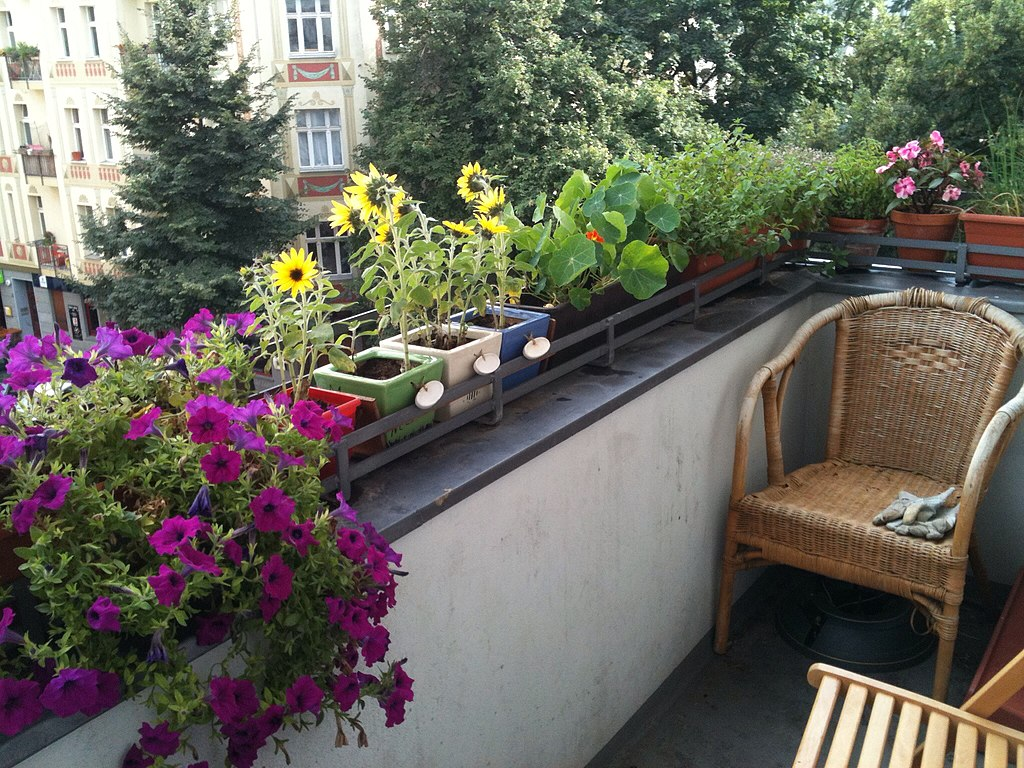
\includegraphics[width=0.5\textwidth]{images/Balkongarten.jpeg}
	\caption[Bild eines Balkongartens mit verschiedenen Balkonkästen.]{
		Bild eines engen Balkongartens mit verschiedenen Balkonkästen, in denen unterschiedliche Pflanzen wachsen.\footnotemark
		}
	\label{pic:balkongarten}
\end{figure}

\footnotetext{Bildquelle: tlcoles, \href{https://creativecommons.org/licenses/by-sa/3.0}{CC BY-SA 3.0}, via Wikimedia Commons}

Balkone sind in Deutschland weitverbreitet und viele Menschen nutzen den begrenzten Platz auf ihren Balkonen, um kleine Gärten anzulegen~\cite{VuMABalkon}.
Ein solcher ist beispielsweise in \cref{pic:balkongarten} zu sehen.
Bei diesen Balkongärten genannten Gärten kommen hauptsächlich Balkonkästen und Blumentöpfe zum Einsatz, aber auch kleine, nicht begehbare Gewächshäuser sind möglich.
Diese Gartenart zeichnet mehrere Aspekte aus.
Wie in \cref{pic:balkongarten} zu sehen, ist der Platz in vielen Fällen begrenzt, weshalb mögliche Smart Gardening Lösungen kompakt sein sollten.
Auf diesem Balkon sollte die Lösung beispielsweise nicht den Laufweg blockieren.
Als weiterer Aspekt gibt es keine Möglichkeit, Pflanzen direkt in den Boden zu pflanzen, sie müssen in Töpfen oder Kästen wachsen.
Da Töpfe und Balkonkästen Wasser schlechter halten als der Boden, ist hier eine Bewässerung besonders wichtig.
Die eben genannten Aspekte gelten analog auch für die deutlich selteneren Dachterrassen, mit dem Unterschied, dass diese meist größer sind.

\subsubsection{Gewächshaus}

\begin{figure}[!htb]
	\centering
	\includegraphics[width=0.4\textwidth]{images/Gewächshaus-Glas.jpg}
	\includegraphics[width=0.4\textwidth]{images/Gewächshaus-Folie.jpg}
	\caption[Bilder eines Glasgewächshauses und eines Foliengewächshauses.]{
		Zwei Bilder von Gewächshäusern.
		Auf dem linken Bild ist ein mittelgroßes Glasgewächshaus zu sehen.
		Es ist deutlich ersichtlich, dass es fest installiert ist, da der untere Teil gemauert und der obere Teil aus Glas ist.
		Die Dachflächenfenster können geöffnet werden.
		Die Pflanzen im Gewächshaus sind in Töpfen und Kästen gepflanzt.\\
		Auf dem rechten Bild ist ein Foliengewächshaus zu sehen.
		Dieses besteht aus einem Metallgerüst, das mit Folie bespannt ist, wobei auch die Tür aus Metall und Folie besteht.
		Abgesehen von der Tür gibt es keine beweglichen Teile.
		Die Pflanzen im Gewächshaus sind direkt in den Boden gepflanzt.\footnotemark
		}
	\label{pic:gewächshaus}
\end{figure}

Ein Gewächshaus ist eine kontrollierte Umgebung, die der Herstellung bestmöglicher Bedingungen für Pflanzenwachstum dient.
Dementsprechend kann diese Umgebung von Smart Gardening profitieren.
Es gibt kleine und große Gewächshäuser, die sowohl privat als auch kommerziell genutzt werden.
Die Anforderungen einer kommerziellen Nutzung sind dabei höher als die einer privaten Nutzung, wie eine höhere Zuverlässigkeit, da ein Ausfall zu hohen finanziellen Verlusten führen kann.

Gewächshäuser können in einfache und günstige Foliengewächshäuser sowie teure und fest verbaute Glasgewächshäuser unterteilt werden.
In \cref{pic:gewächshaus} sind beispielhaft ein Glasgewächshaus und ein Foliengewächshaus zu sehen.
Auch wenn es sich bei beiden um Gewächshäuser handelt, so gibt es doch viele Unterschiede, insbesondere bezogen auf Smart Gardening.
So ist ein Glasgewächshaus fest installiert und die Pflanzen sind in Töpfe und Kästen gepflanzt.
Ein Foliengewächshaus hingegen ist mobil und die Pflanzen sind direkt in den Boden gepflanzt.
Daraus ergeben sich unterschiedliche Anforderungen an Smart Gardening Lösungen, wobei die Anforderungen eines Foliengewächshauses denen eines Beetes ähneln.
Dies ergibt sich daraus, dass ein Foliengewächshaus praktisch ein überdachtes Beet ist, wie in \cref{pic:gewächshaus} zu sehen.
Daher fokussiert sich dieser Abschnitt auf Glasgewächshäuser.

\footnotetext{Bildquellen:\\
	Links: Vanellus Foto, \href{https://creativecommons.org/licenses/by-sa/3.0}{CC BY-SA 3.0}, via Wikimedia Commons,\\
	Rechts: Selso, \href{https://creativecommons.org/licenses/by-sa/2.5}{CC BY-SA 2.5}, via Wikimedia Commons
}

Ziel eines Gewächshauses ist es, Erträge von Pflanzen in einem geschützten Raum mit kontrollierten Bedingungen zu maximieren.
So müssen die Sensoren möglichst genau und die Aktuatoren möglichst fein regelbar sein.
Gleichzeitig ist die Umgebung besonders feucht und warm.
In einem Gewächshaus wachsen viele Pflanzen auf engem Raum, was in \cref{pic:gewächshaus} erahnt werden kann, wobei es gleichzeitig viele Parameter zu überwachen und zu steuern gibt.
So sind etwa Temperatur, Luftfeuchtigkeit, Licht, CO$_2$-Gehalt, Wasserstand und Nährstoffgehalt zu überwachen und zu steuern.
Genaueres dazu wird in \cref{sec:gartenlement-gewächshaus} erläutert.
Aufgrund des begrenzten Platzes mit vielen Sensoren und Aktuatoren ist es wichtig, dass diese nicht stören.
Gleichzeitig ist alles im Gewächshaus besser gegen die Elemente geschützt als im Freien, wo beispielsweise Regen und Wind die Sensoren und Aktuatoren beschädigen können.

\subsubsection{Vorgarten}
\begin{figure}[!htb]
	\centering
	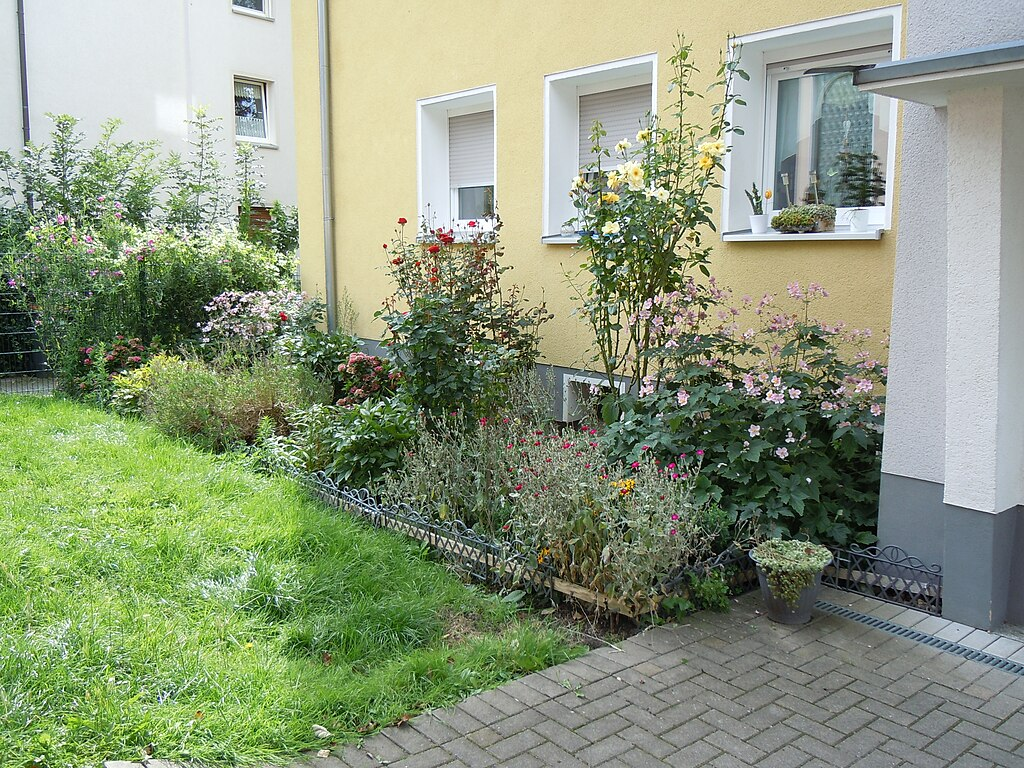
\includegraphics[width=0.5\textwidth]{images/Vorgarten.jpg}
	\caption[Bild eines typischen Vorgartens eines Mehrfamilienhauses.]{Bild eines typischen Vorgartens eines Mehrfamilienhauses.\footnotemark}
	\label{pic:vorgarten}
\end{figure}

\footnotetext{Bildquelle: Sebastian Martin Dicke, \href{https://creativecommons.org/licenses/by-sa/4.0}{CC BY-SA 4.0}, via Wikimedia Commons}

Viele Häuser weisen Vorgärten auf, insbesondere Reihenhäuser und Einfamilienhäuser, aber auch Mehrfamilienhäuser können Vorgärten haben, wie in \cref{pic:vorgarten} zu sehen.
Dieser ist meist relativ klein und dient der Verschönerung des Hauses aus der Sicht der Straße.
Demzufolge ist es wünschenswert, wenn die Smart Gardening Lösungen möglichst unauffällig sind und sich in die Umgebung integrieren lassen.
Im Beispiel des Vorgartens in \cref{pic:vorgarten} ist ein Rasen und ein Blumenbeet zu sehen, wobei auch andere Elemente wie Bäume, Sträucher und Steine möglich sind.
Für eine unauffällige Integration sollte die Smart Gardening Lösung möglichst klein und leise sein, wobei dies nicht immer möglich sein wird.
Da Vorgärten häufig von der Straße aus einsehbar sind, hilft eine unauffällige Integration auch gegen Diebstahl und Vandalismus.

\pagebreak

\subsubsection{Kleingarten}
\begin{figure}[!htb]
	\centering
	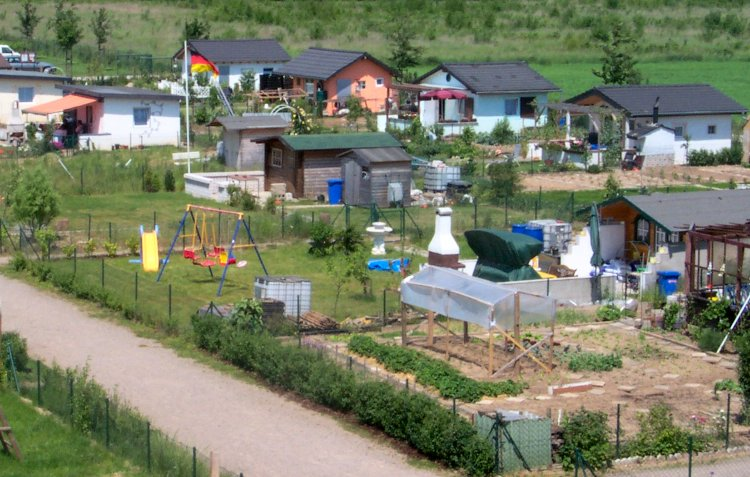
\includegraphics[width=0.5\textwidth]{images/Kleingarten.jpg}
	\caption[Bild von mehreren Parzellen einer Kleingartenanlage.]{
		Bild von mehreren Parzellen einer Kleingartenanlage.
		Zu sehen ist dabei die unterschiedliche Nutzung, die mittlere Parzelle wird als Spielplatz genutzt, während die vordere Parzelle für den Gemüseanbau genutzt wird.\footnotemark
	}
	\label{pic:kleingarten}
\end{figure}

\footnotetext{Bildquelle: Journey234, Public Domain, via Wikimedia Commons}

Bei einem Kleingarten, auch Schrebergarten genannt, handelt es sich um eine Parzelle in einer größeren Gartenanlage, wie sie beispielsweise in \cref{pic:kleingarten} zu sehen ist.
Kleingärten sind in Vereinen organisiert und die Mitglieder unterliegen der Kleingartensatzung des Vereins, woraus sich häufig spezielle Verpflichtungen und Einschränkungen ergeben, die bei Smart Gardening Lösungen berücksichtigt werden müssen.
Dabei kann es sich beispielsweise um Nutzungseinschränkungen für bestimmte Gerätetypen, Lärmschutz oder Verbot von Solaranlagen handeln.
Auch die Versorgung mit Strom und Wasser ist in verschiedenen Kleingartenanlagen unterschiedlich geregelt, wenn diese überhaupt vorhanden ist.
Es kann auch Verpflichtungen zur Art der Nutzung geben wie die Pflicht zum Anbau von Obst und Gemüse.
Daraus ergeben sich Anforderungen an die Flexibilität der Smart Gardening Lösungen.
Gleichzeitig muss beachtet werden, dass einige Smart Gardening Lösungen durch die Einschränkungen nicht oder nur eingeschränkt nutzbar sind.

Der Kleingarten wird auf verschiedene Arten und Weisen genutzt.
So nutzen einige Kleingärtner diesen zum Anbau von Obst und Gemüse, andere ihn zur Entspannung, was gut in \cref{pic:kleingarten} zu sehen ist.
Auch Imker sind in vielen Kleingärten vertreten, da der Imker von den vielen Pflanzen und die Kleingärtner von den Bienen profitieren.
Da diese Gartenart räumlich vom Wohnort getrennt ist, kann es sein, dass es immer wieder zu längeren Abwesenheiten des Hobbygärtners kommt.
Daher ist es von Vorteil, wenn die Smart Gardening Lösung auch ohne ständige Anwesenheit funktioniert.

\subsubsection{Hintergarten}
\begin{figure}[!htb]
	\centering
	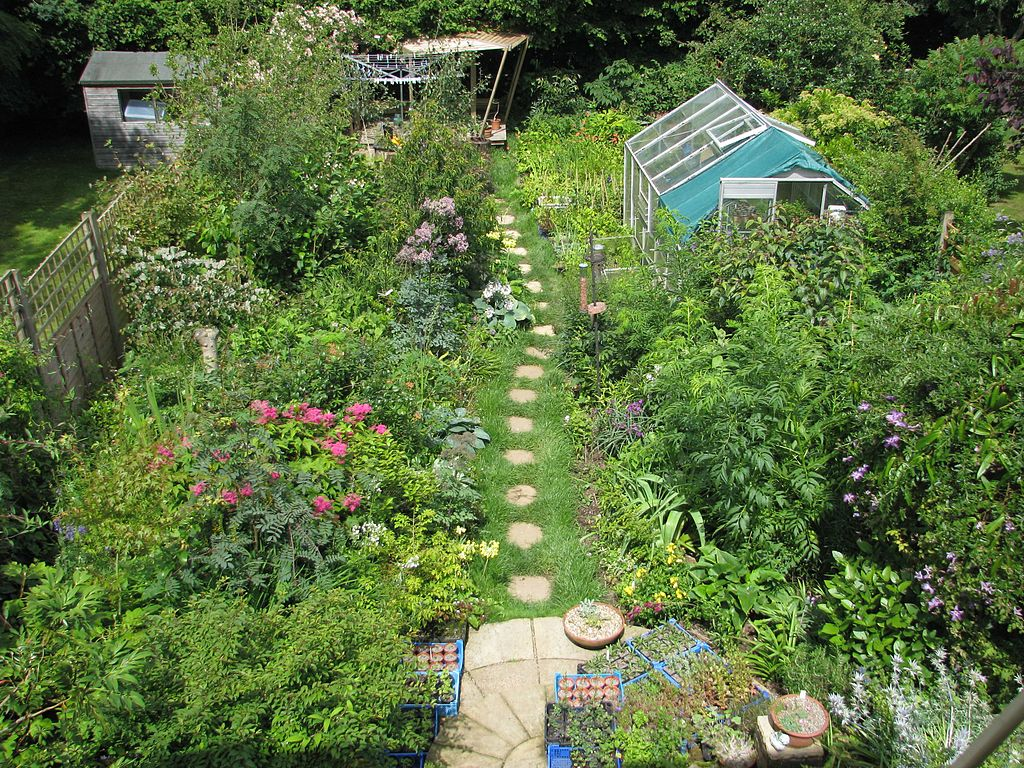
\includegraphics[width=0.5\textwidth]{images/Hintergarten.jpg}
	\caption[Bild eines kleinen, dicht bewachsenen Hintergartens.]{
		Bild eines kleinen, dicht bewachsenen Hintergartens.
		In diesem befinden sich viele verschiedene Pflanzen, ein Glasgewächshaus, eine Gartenhütte und eine Wäschespinne.
		Der Garten weist aufgrund des Bewuchses mit anderen Pflanzen keine größere Rasenfläche auf.\footnotemark
	}
	\label{pic:hintergarten}
\end{figure}

Viele Reihenhäuser und Einfamilienhäuser weisen einen Hintergarten auf.
Dieser ist meist eingezäunt und kann ansonsten viele verschiedene Formen und Größen aufweisen, wie in \cref{pic:hintergarten} zu sehen.
Dabei ist dieser häufig größer als ein Vorgarten, weshalb hier umfangreichere Smart Gardening Lösungen umgesetzt werden können.
Gleichzeitig sind große Teile des Gartens weiter vom Haus entfernt, was in dem Beispielbild gut zu sehen ist.

Normalerweise hat ein solcher Garten einen Rasen, welcher regelmäßig gemäht werden muss, wofür sich Mähroboter anbieten.
Auch verschiedene Beete und Bäume sind hier häufig zu finden, was in \cref{pic:hintergarten} gut zu sehen ist.
Je nach Größe des Gartens erfordern diese viel Pflege und Aufmerksamkeit, weshalb Smart Gardening Lösungen hier eine große Hilfe sein können.
Insbesondere die Bewässerung muss in Trockenperioden regelmäßig erfolgen, wofür sich automatische Bewässerungssysteme anbieten.
Hierbei ist es wichtig, dass die Sensoren und Aktuatoren auch in den hinteren Teilen des Gartens zuverlässig funktionieren.
Weiterhin weisen viele Hintergärten ein Gartenhaus zur Lagerung von unter anderem Werkzeug auf und einige haben auch ein Gewächshaus für den Anbau von Pflanzen, wie in \cref{pic:hintergarten} zu sehen.

\footnotetext{Bildquelle: peganum, \href{https://creativecommons.org/licenses/by-sa/2.0}{CC BY-SA 2.0}, via Wikimedia Commons}

Eine besondere Art des Hintergartens ist der große Garten, wobei die Abgrenzung in der Realität fließend ist.
Hier wird analog zu~\cite{grosserGarten} ein Garten als großer Garten bezeichnet, wenn er größer als 1.000 Quadratmeter ist.
Große Gärten weisen besondere Herausforderungen auf.
Um einen solchen Garten vollständig mit Smart Gardening ausstatten zu können, muss eine solche Lösung skalierbar sein.
Außerdem hat ein großer Garten potenziell mehr verschiedene Elemente, die mit unterschiedlichen Sensoren eingebunden werden wollen.
Welche Smart Gardening Lösungen für die jeweiligen Elemente geeignet sind, wird in den entsprechenden Abschnitten erläutert.

\subsubsection{Landschaftsgarten}
\begin{figure}[!htb]
	\centering
	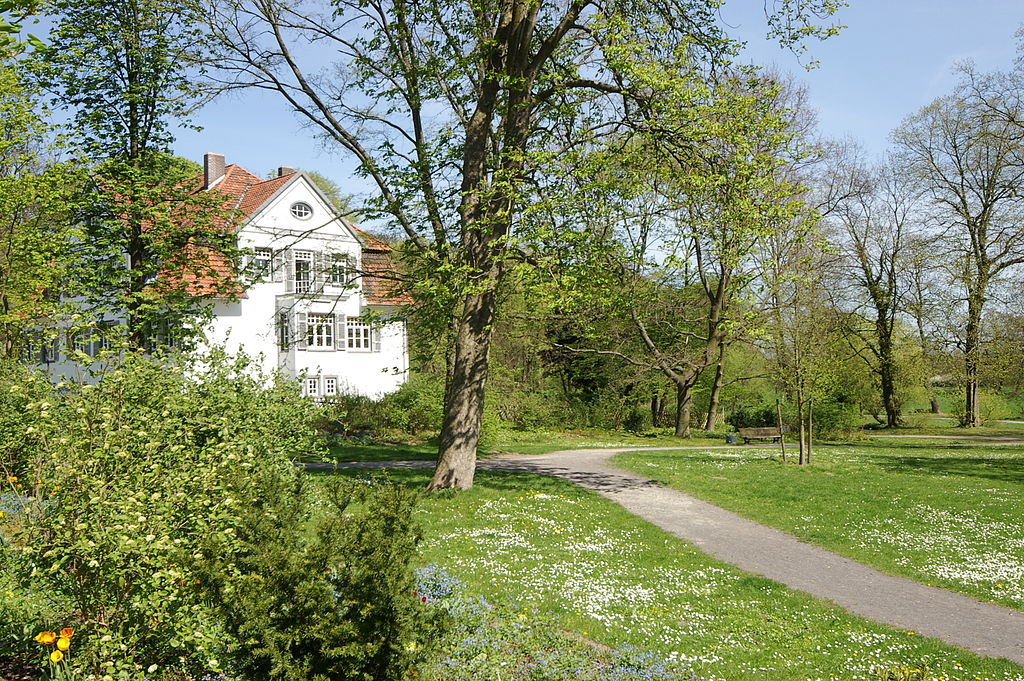
\includegraphics[width=0.5\textwidth]{images/Landschaftsgarten.jpg}
	\caption[Bild eines Landschaftsgartens mit einem Weg, Bäumen und Büschen.]{
		Bild eines Landschaftsgartens mit einem Weg und mehreren Bäumen und Büschen.\footnotemark
	}
	\label{pic:landschaftsgarten}
\end{figure}

Landschaftsgärten sind größere Gärten, die normalerweise nicht einem Haushalt zugeordnet sind, wie in Parks.
Ein Beispiel dafür ist in \cref{pic:landschaftsgarten} zu sehen, wobei dieser Landschaftsgarten von einem Weg durchzogen ist.
Sie dienen der Verschönerung und Erholung, sind meist der Öffentlichkeit zugänglich und werden häufig von professionellen Gärtnern gepflegt.
Daher sind hier Smart Gardening Lösungen sinnvoll, die den Gärtner in seiner Arbeit unterstützen, ihm also Arbeit abnehmen, ihm Kosten oder Zeit sparen oder die Qualität der Arbeit verbessern.
Aufgrund der öffentlichen Nutzung besteht eine erhöhte Gefahr von Diebstahl oder Vandalismus, weshalb die Smart Gardening Lösungen robust und sicher sein müssen.
Gleichzeitig sollten sie sich unauffällig in die Umgebung integrieren lassen, um das Erscheinungsbild nicht zu stören und gleichzeitig diese Gefahr zu minimieren.
Da Landschaftsgärten meistens größer sind als andere Gärten, müssen die Sensoren und Aktuatoren flächenmäßig skalierbar eingesetzt werden können.

\footnotetext{Bildquelle: Ingo Rickmann Ricki, \href{https://creativecommons.org/licenses/by-sa/2.5}{CC BY-SA 2.5}, via Wikimedia Commons}

\subsubsection{Landwirtschaft}
Die Landwirtschaft ist ein weiteres Umfeld, in dem Smart Gardening eingesetzt werden kann.
Aufgrund der Diversität dieses Umfelds und dem Fokus auf vor allem Hobbygärtner und nachrangig professionelle Gärtner wird hier nur ein kurzer Überblick gegeben.
Des Weiteren werden die Anforderungen an Smart Gardening zwar theoretisch genannt, aber nicht in die Anforderungsmenge aufgenommen.
Landwirtschaft setzt sich zusammen aus dem wirtschaftlichen Betrieb von Ackerbau und Viehwirtschaft.
Dabei gibt es verschiedene Formen von Landwirtschaft, die sich in der Größe und der Art der Bewirtschaftung unterscheiden.
Der Unterschied zur Gartenarbeit liegt in der Größe und der kommerziellen Nutzung.

\begin{figure}[!ht]
	\centering
	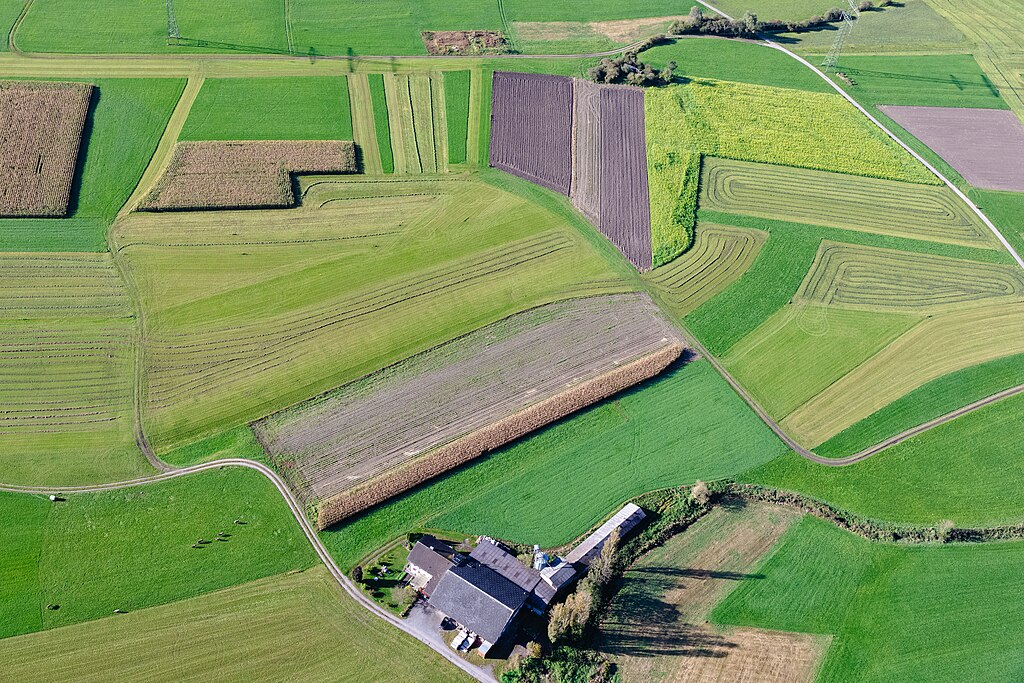
\includegraphics[width=0.5\textwidth]{images/Landwirtschaft.jpg}
	\caption[Bild einer kleinen landwirtschaftlich genutzten Fläche.]{
		Bild einer kleinen landwirtschaftlich genutzten Fläche.
		Außerdem ist ein Haus mit abgebildet.\footnotemark
	}
	\label{pic:landwirtschaft}
\end{figure}

In \cref{pic:landwirtschaft} ist eine kleine landwirtschaftlich genutzte Fläche zu sehen, die im Vergleich zu Gärten deutlich größer ist, gleichzeitig gibt es noch viel größere landwirtschaftliche Flächen.
Die Größe ist dabei eine Herausforderung für Smart Gardening, da die Sensoren und Aktuatoren entsprechend skalierbar sein müssen.
Wird etwa ein automatisches Bewässerungssystem eingesetzt, so muss die gesamte Fläche mit entsprechenden Feuchtigkeitssensoren und Bewässerungsdüsen ausgestattet werden.
Diese großflächige Ausstattung ist aufwendig und teuer, weshalb hier eine hohe Zuverlässigkeit und Effizienz gefordert ist.
Das Budget ist zwar größer als bei Gärtnern, aber die Fläche ist auch um ein Vielfaches größer.

\footnotetext{Bildquelle: Herbert Heim, \href{https://creativecommons.org/licenses/by-sa/4.0}{CC BY-SA 4.0}, via Wikimedia Commons}

\subsubsection{Zusammenfassung der Gartenarten}
Gerade wurde die Vielfalt der verschiedenen Gartenarten dargestellt.
Diese Liste ist nicht vollständig und kann es auch nicht sein, deckt aber die häufigsten Gärten ab.
Andere Gartenarten können als Unterarten oder Kombinationen dieser Gartenarten betrachtet werden.
So hat etwa ein japanischer Garten Elemente eines Landschaftsgartens und eines Vorgartens.

Dabei gibt es viele Gemeinsamkeiten, aber auch viele Unterschiede zwischen den verschiedenen Gartenarten.
Alle Gartenarten können in verschiedenen Arten von Smart Gardening Lösungen profitieren, wobei die Anforderungen an diese unterschiedlich sind.
Hierbei kann es sich beispielsweise um Arbeitserleichterungen, Kosteneinsparungen oder Ertragssteigerungen handeln.
Smart Gardening Lösungen benötigen für die meisten Gartenarten eine zusätzliche Strom- und Wasserversorgung, wobei die Internetverbindung in den meisten Fällen über WAN erfolgt.
In fast allen Gärten sind Schädlinge und andere Tiere ein Problem, weshalb eine Detektion und gegebenenfalls Verjagung notwendig ist.

\pagebreak

Gleichzeitig sind alle Gärten in unterschiedlicher Intensität den Elementen ausgesetzt, weshalb die Smart Gardening Lösungen robust sein müssen.
In den verschiedenen Gartenarten können nun unterschiedliche Gartenelemente vorkommen, auf die im nächsten Abschnitt eingegangen wird.


\subsection{Gartenelemente}
In diesem Abschnitt werden verschiedene Gartenelemente, die teilweise schon erwähnt wurden, erklärt und im Kontext von Smart Gardening analysiert.
Sie bringen eigene Eigenschaften und Anforderungen an Smart Gardening mit sich.
Dazu gehört, was diese Elemente ausmacht und was beachtet werden muss.
Zunächst werden gemeinsame Aspekte der verschiedenen Gartenelemente betrachtet.
Danach wird die folgende ausgewählte Teilmenge der Gartenelemente betrachtet, welche nach Ähnlichkeit sortiert ist: Rasen, Beet, Baum, Pflanzentopf, Gewächshaus, Regentonne, Brunnen, Gartenteich, Pool, Gartenhaus, Gehege / Stall, Bienenstock und Kompost.

Für die Analyse werde die Gartenelemente zunächst erklärt, danach werden sie voneinander abgegrenzt und ihre Besonderheiten herausgestellt.
Zum Schluss wird betrachtet, von welchen Messungen und Automatisierungen sie profitieren können.
Nach den einzelnen Gartenelementen folgt eine Zusammenfassung mit verschiedenen Tabellen zur Übersicht über die Gartenelemente.

\subsubsection{Gartenelementübergreifende Aspekte}
Zunächst werden gemeinsame Aspekte der verschiedenen Gartenelemente betrachtet, welche auf viele Gartenelemente zutreffen.
Fast alle Gartenelemente sind den Elementen ausgesetzt, wozu unter anderem Regen, Schnee, Wind, Sonne und Temperaturschwankungen zählen.
Ein automatisches Bewässerungssystem ist etwa der Luft- und Bodenfeuchtigkeit und Regen ausgesetzt, was aufgrund der Elektronik und Rost ein Problem darstellen kann.
Weiterhin ist ein Bewässerungssystem im Garten der Sonne ausgesetzt, was über längere Zeit zu Schäden führen kann.

Pflanzengartenelemente wie Rasen und Beete sind sich in vielen Aspekten besonders ähnlich.
Dazu gehört unter anderem die Bewässerung der Pflanzen, die notwendig für diese ist, wenn sie nicht durch Regen ausreichend versorgt werden.
Die Bewässerung kann durch ein automatisches Bewässerungssystem übernommen werden.
Die Koppelung dieser Bewässerung an Bodenfeuchtigkeitssensoren sowie an Wetterdaten kann die Bewässerung optimieren und so die Pflanzen besser versorgen.
Dabei kann die Bewässerung auch an die Art der Pflanzen angepasst werden, da verschiedene Pflanzen unterschiedliche Wassermengen benötigen.
Frost kann solche Bewässerungssysteme potenziell beschädigen, weshalb eine Temperaturmessung in Kombination mit Wetterdaten helfen kann, Frost zu erkennen und das Bewässerungssystem abzuschalten.
Gleichzeitig kann der Nutzer über diese Gefahr informiert werden, damit er eventuelle weitere Gegenmaßnahmen einleiten kann.
Als Wasserquelle für ein solches Bewässerungssystem können ein Außenwasseranschluss, ein Brunnen oder eine Wassertonne dienen.

Ein weiterer Aspekt ist die Düngung der Pflanzen, welche regelmäßig erfolgen muss, um die Pflanzen optimal zu versorgen.
Hierbei ist zu beachten, dass falsches Düngen zum Einen die Umwelt belasten und zum Anderen die Pflanzen schädigen kann~\cite{RasenDuenger}.
Durch Messungen kann etwa der Stickstoffgehalt und Phosphorgehalt im Boden gemessen werden, woraus abgeleitet werden kann, wann und wie viel Dünger benötigt wird.
Hierbei sollte bei der Auswahl der überwachten Stoffe im Boden darauf geachtet werden, dass diese relevant für die Pflanzen sind.
Ein intelligentes System kann basierend auf diesen Daten den Nutzer informieren, wann und wie viel gedüngt werden soll.
Auch der pH-Wert des Bodens ist wichtig, weshalb der Nutzer bei einer größeren Abweichung vom Idealwert informiert werden kann.
So kann er rechtzeitig Gegenmaßnahmen einleiten, wie das Kalken des Bodens.

\subsubsection{Gartenelement Rasen}
\begin{figure}[!htb]
	\centering
	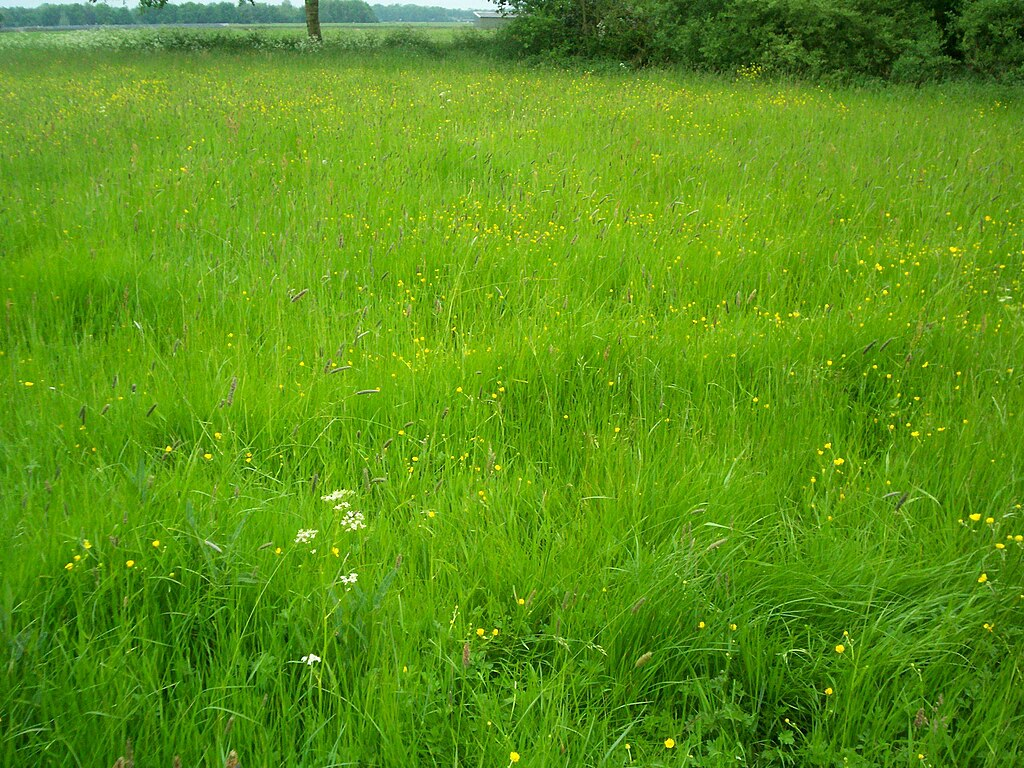
\includegraphics[width=0.5\textwidth]{images/Rasen.jpg}
	\caption[Bild eines wild wachsenden Rasens, der seit Längerem nicht gemäht wurde.]{
		Ein wild wachsender Rasen, der seit Längerem nicht gemäht wurde.
		Auch Blumen wachsen auf der Rasenfläche.\footnotemark
	}
	\label{pic:rasen}
\end{figure}

\footnotetext{Bildquelle: Natubico, \href{https://creativecommons.org/licenses/by-sa/3.0}{CC BY-SA 3.0}, via Wikimedia Commons}

Ein Rasen ist eine weitverbreitete Vegetationsdecke aus verschiedenen Gräsern, wie sie in \cref{pic:rasen} zu sehen ist.
Sie wird häufig in Gärten und Parks angelegt und muss regelmäßig gepflegt werden.
Zu dieser Pflege gehört das Mähen, das Bewässern und das Düngen.
Dabei gibt es verschiedene Möglichkeiten den Rasen zu mähen, wie mit Tieren wie Ziegen, verschiedenen Arten von Rasenmähern und neuerdings auch mit Mährobotern.
Das manuelle Mähen mit einem Rasenmäher ist zeitaufwendig und anstrengend, weshalb automatische Mähroboter eine gute Alternative darstellen.
Diese können auf verschiedene Arten gesteuert werden, wozu Regeln, Apps und verschiedene Schnittstellen gehören.
Eine solche Regel kann einfach zeitbasiert, aber auch komplex abhängig von Sensorwerten sein.
Durch komplexere Regeln kann das Mähen an die Situation angepasst werden.
Rasen wächst bei unterschiedlichen Temperaturen unterschiedlich schnell und ist bei hohen Temperaturen empfindlicher, weshalb die Mähfrequenz angepasst werden sollte.
Dabei können sowohl Wetterdaten als auch Sensoren für die Temperatur helfen.
Die Bewässerung kann von automatischen Bewässerungssystemen übernommen werden, wie in den gartenelementübergreifenden Aspekten beschrieben.
Auch die Düngung des Rasens kann, wie in den gartenelementübergreifenden Aspekten beschrieben, automatisiert unterstützt werden.

\subsubsection{Gartenelement Beet}
\begin{figure}[!htb]
	\centering
	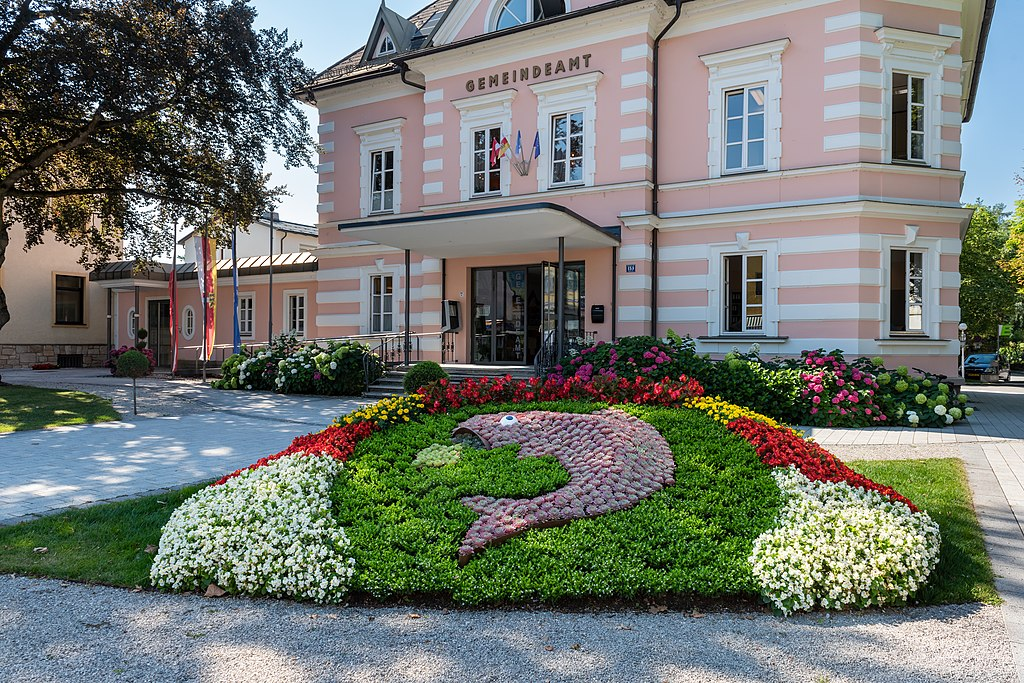
\includegraphics[width=0.49\textwidth]{images/Blumenbeet.jpg}
	\includegraphics[width=0.49\textwidth]{images/Gemüsebeet.jpg}
	\caption[Bilder von verschiedenen Beeten.]{Zwei Bilder von verschiedenen Beeten.
		Auf dem linken Bild ist ein Hügel-Blumenbeet zu sehen, welches mit den Blumen ein Muster bildet.
		Auf der rechten Seite ist Boden-Gemüsebeet zu sehen, in welchem in langen Reihen verschiedene Gemüsesorten wachsen.\footnotemark
	}
	\label{pic:beet}
\end{figure}

\footnotetext{Bildquellen:\\
	Links: Johann Jaritz, \href{https://creativecommons.org/licenses/by-sa/4.0}{CC BY-SA 4.0}, via Wikimedia Commons\\
	Rechts: Burkhard Mücke, \href{https://creativecommons.org/licenses/by-sa/4.0}{CC BY-SA 4.0}, via Wikimedia Commons
}

Ein Beet ist ein Bereich, in dem Pflanzen angebaut werden.
Es gibt verschiedene Arten und Formen von Beeten, wie in \cref{pic:beet} zu sehen.
Bei der Unterscheidung von Beeten kann nach der Art der Pflanzen und nach der Form unterschieden werden, wobei beliebige Kombinationen möglich sind.
So ist in \cref{pic:beet} links ein Blumenbeet als Hügelbett zu sehen, während rechts ein Gemüsebeet als Bodenbeet zu sehen ist.

Bei der Art der Pflanzen sind unter anderem Blumenbeete, Obst- und Gemüsebeete, Kräuterbeete und Staudenbeete möglich.
Je nach Art der Pflanzen können sich die Anforderungen an Smart Gardening geringfügig unterscheiden.
So dient ein Blumenbeet meist der Verschönerung des Gartens, weshalb hier die Optik eine größere Rolle spielt.
Ein Gemüsebeet hingegen dient der Selbstversorgung, weshalb hier die Menge und Qualität der Ernte eine größere Rolle spielen.
Gleichzeitig ähneln sich die Anforderungen an die Pflege, insbesondere bei der Bewässerung, dem Düngen und dem Entfernen von Unkraut.
Daher gelten unabhängig von der Art und Bepflanzung die gartenelementübergreifenden Aspekte für die automatische Bewässerung und Düngung.
Weiterhin benötigen verschiedene Pflanzen unterschiedliche Licht- und Temperaturbedingungen~\cite*{RosenTemperatur}.
Durch die Nutzung von Wetterdaten in Kombination mit Temperaturmessungen kann der Nutzer informiert werden, wenn die Bedingungen nicht optimal sind und es zu warm oder zu kalt ist oder wird.
Die Blüten und Früchte von Pflanzen können beispielsweise bei Frost Schaden nehmen, weshalb eine zeitige Reaktion des Nutzers notwendig ist.
In solchen Fällen kann der Nutzer handeln, um die Bedingungen zu verbessern, indem er die Pflanzen beispielsweise abdeckt, um die Temperatur zu halten und Frost zu vermeiden.

Für die Form gibt es verschiedene Möglichkeiten wie Hügelbeete, Bodenbeete und Hochbeete, wobei diese Einfluss auf beispielsweise die Bewässerung haben
Hochbeete benötigen bei gleicher Bepflanzung eine andere Bewässerung als Bodenbeete, da das Wasser im Hochbeet schneller abläuft.
Gleichzeitig sorgt die Erhöhung auch dafür, dass für das Bewässerungssystem Gravitation nicht mehr genutzt werden kann und somit auf eine andere Art Wasserdruck erzeugt werden muss.
Daher ist es wichtig, dass Smart Gardening Lösungen an die Form des Beetes angepasst werden können.
Auch Aspekte wie die Düngung können von der Form des Beetes abhängen, da Hügelbeete wie in \cref{pic:beet} häufig mit Kompost gebaut werden und somit der Düngebedarf unterschiedlich ist.

\subsubsection{Gartenelement Baum}
\begin{figure}[!htb]
	\centering
	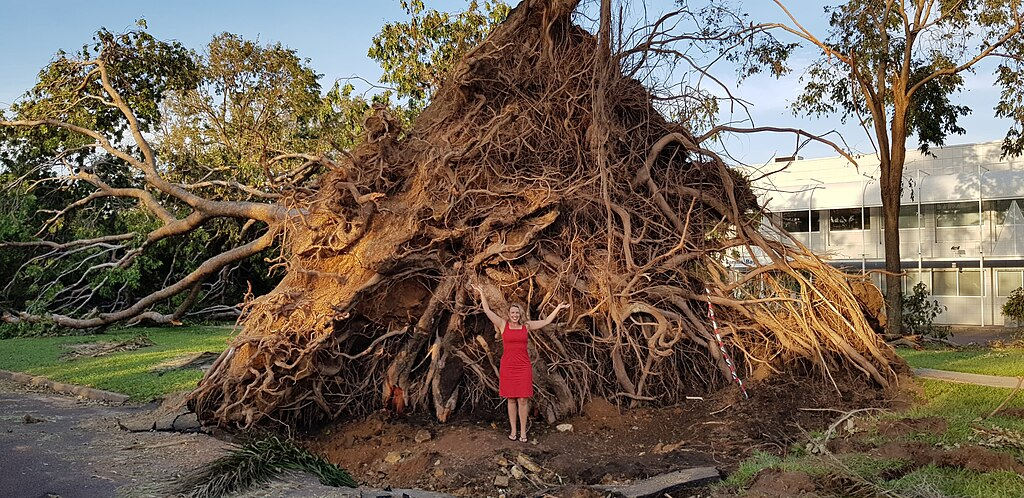
\includegraphics[width=0.7\textwidth]{images/Wurzeln.jpg}
	\caption[Bild eines umgekippten Baumes.]{
		Bild eines umgekippten Baumes.
		Der Baum liegt entwurzelt auf der Seite, wodurch das tiefe Wurzelwerk sichtbar wird.\footnotemark
	}
	\label{pic:baum}
\end{figure}

\footnotetext{Bildquelle: Kclovelock, \href{https://creativecommons.org/licenses/by-sa/4.0}{CC BY-SA 4.0}, via Wikimedia Commons}

Bäume sind Holzgewächse, die in Gärten und Wäldern vorkommen, hunderte Jahre alt und über zehn Meter groß werden können.
Auch Bäume benötigen Pflege, um gesund zu bleiben.
Insbesondere junge Bäume müssen regelmäßig gegossen werden, aber auch ältere Bäume können von einer Bewässerung in Trockenperioden profitieren.
Die automatische Bewässerung, wie in den gartenelementübergreifenden Aspekten beschrieben, kann hier nicht eingesetzt werden.
Bäume haben ein tiefes Wurzelsystem wie in \cref{pic:baum} zu sehen, weshalb die Messung der Bodenfeuchtigkeit in der Nähe des Baumes nicht aussagekräftig ist und somit übermäßig gegossen werden kann.
Daher ist hier ein größerer Fokus auf die Wetterdaten wichtig, wobei diese mit Informationen über das Alter und die Art des Baumes kombiniert werden können.
Daraus kann abgeleitet werden, wie viel und wie oft der Baum gegossen werden muss.
Außerdem benötigen Bäume aufgrund ihrer Größe im Vergleich zu anderen Pflanzen mehr Wasser, weshalb dies bei der Wahl der Wasserquelle berücksichtigt werden muss.

\subsubsection{Gartenelement Pflanzentopf}
\begin{figure}[!htb]
	\centering
	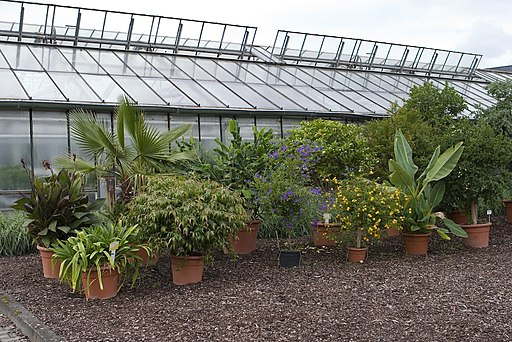
\includegraphics[width=0.5\textwidth]{images/Topf.jpg}
	\caption[Bild einer Reihe von Pflanzentöpfen.]{
		Bild einer Reihe von Pflanzentöpfen.
		Die Töpfe sind verschieden groß und mit unterschiedlichen Pflanzen bepflanzt.\footnotemark
	}
	\label{pic:topf}
\end{figure}

\footnotetext{Bildquelle: Martin Bahmann, \href{https://creativecommons.org/licenses/by-sa/3.0}{CC BY-SA 3.0}, via Wikimedia Commons}

Ein Pflanzentopf ist ein Behälter, der zum Anpflanzen von Pflanzen verwendet wird.
Er ist in verschiedenen Größen und Materialien erhältlich wie in \cref{pic:topf} und kann im Innen- oder Außenbereich verwendet werden.
Töpfe werden für die Kultivierung von Pflanzen auf Terrassen, Balkonen oder in Gärten eingesetzt.
Smart Gardening kann eingesetzt werden, um die Pflege von Pflanzen in Töpfen zu erleichtern.
Für die Bewässerung und Düngung gelten die gartenelementübergreifenden Aspekte.
Weiterhin können die Pflanzen von Licht- und Temperaturmessungen profitieren, da verschiedene Pflanzen unterschiedliche Licht- und Temperaturbedingungen benötigen.
Durch die Messung dieser Werte kann der Nutzer informiert werden, wenn die Bedingungen nicht optimal sind.
Je nach Position des Pflanzentopfes können auch Wetterdaten relevant sein, um etwa eine Warnung auszugeben, wenn Sturm oder Hagel droht.
In so einem Fall können die Pflanzen geschützt werden.
Diese Smart Gardening Überlegungen für Töpfe können auch auf Balkonkästen und Blumenkästen übertragen werden.

\subsubsection{Gartenelement Gewächshaus}\label{sec:gartenlement-gewächshaus}
Zuvor wurde bereits das Gewächshaus als Gartenart betrachtet.
Nun wird das Gewächshaus als Gartenelement betrachtet, wobei der Fokus auf Glasgewächshäusern liegt wie links in \cref{pic:gewächshaus}.
Als kontrollierte Umgebung kann das Gewächshaus von diverser Sensorik und Aktuatorik profitieren.
Pflanzen haben Temperaturanforderungen für ein gutes Wachstum, weshalb die Temperatur ein wichtiger Faktor ist.
Durch regelmäßige Temperaturmessungen kann überwacht werden, ob die Temperatur den optimalen Bereich verlässt.
Geschieht dies, so kann beispielsweise durch Heizen oder Lüften automatisiert gegengesteuert werden.
Die Luftfeuchtigkeit ist ein weiterer wichtiger Faktor.
Auch hier können Messungen und automatisierte Gegenmaßnahmen eingesetzt werden, wie mit Luftbefeuchtern, Luftentfeuchtern und Lüften.
Da Pflanzen Licht zum Wachsen benötigen, ist die Messung der Lichtintensität wichtig.
Diese Messung kann genutzt werden, um automatisiert die Beleuchtung zu steuern.
Pflanzen profitieren auch von einem erhöhten CO$_2$-Gehalt in der Luft, weshalb es von Vorteil ist diesen zu messen und automatisiert zu steuern~\cite{PflanzenCO2}.
Für die Bewässerung und Düngung gelten die gartenelementübergreifenden Aspekte.
In all diese Maßnahmen können Wetterdaten einfließen.

\subsubsection{Gartenelement Regentonne}
\begin{figure}[!htb]
	\centering
	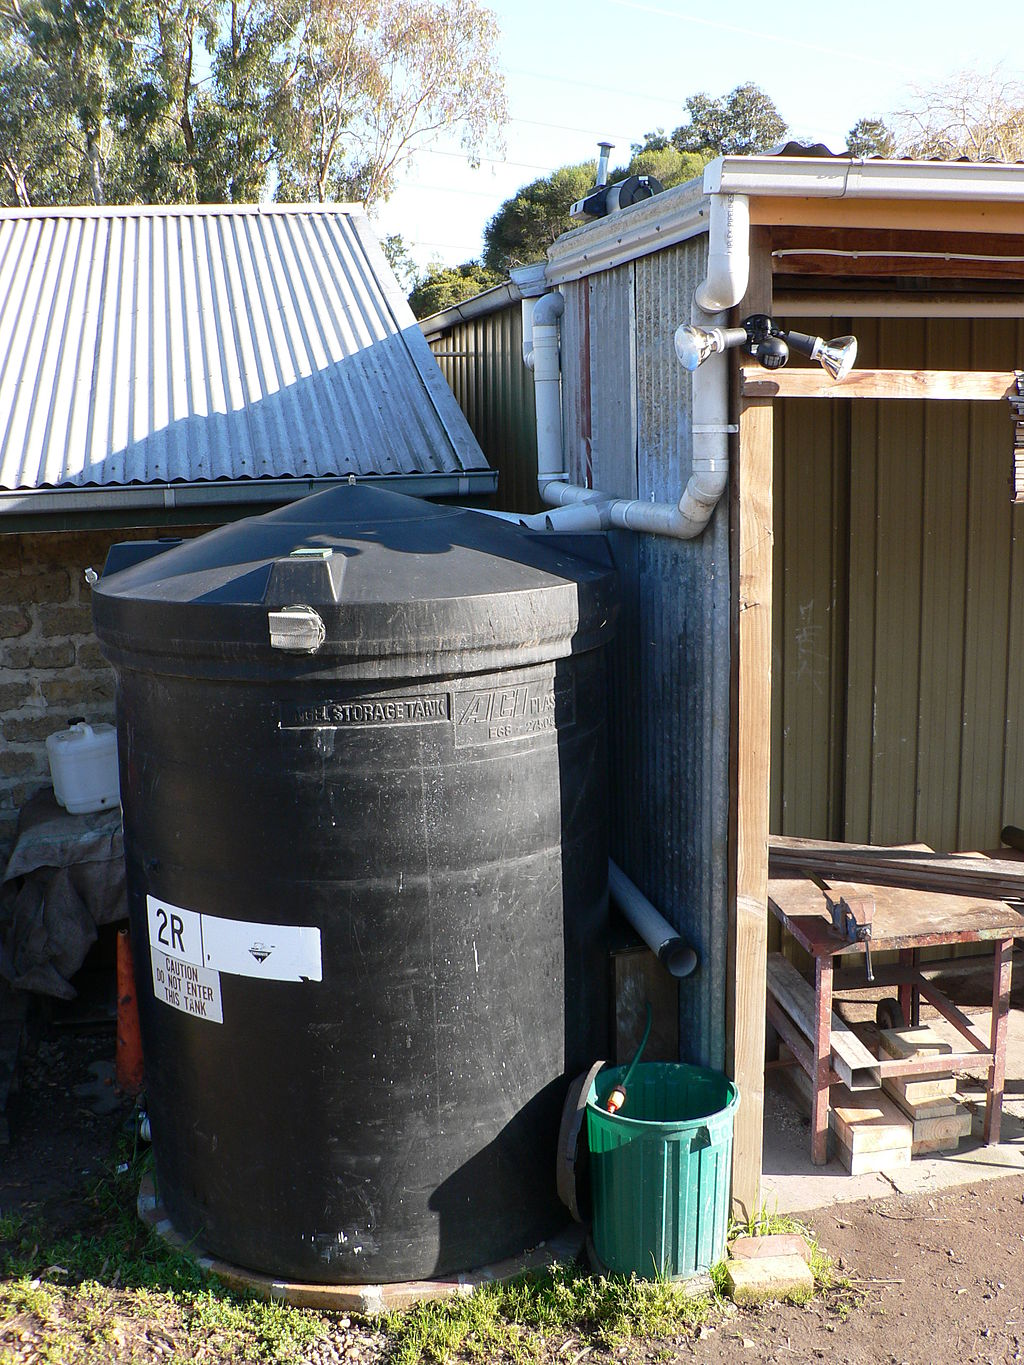
\includegraphics[height=0.4\textheight]{images/Regentonne.jpg}
	\caption[Bild einer Regentonne, die am Deckel einen Zulauf hat.]{
		Bild einer Regentonne, die am Deckel einen Zulauf hat, der von Dachrinnen gefüllt werden kann.\footnotemark
	}
	\label{pic:regentonne}
\end{figure}

\footnotetext{Bildquelle: Pengo, \href{https://creativecommons.org/licenses/by-sa/3.0}{CC BY-SA 3.0}, via Wikimedia Commons}

Eine Regentonne ist ein Behälter, der Regenwasser sammelt.
Wie in \cref{pic:regentonne} zu sehen, wird das Regenwasser zunächst in Dachrinnen gesammelt und dann über Leitungen in eine Regentonne oder einen anderen Behälter geleitet.
Dadurch können große Mengen an Wasser gesammelt werden, insbesondere bei großen Dachflächen und langem und starkem Regen.
Dieses gesammelte Regenwasser kann dann zur Bewässerung von Pflanzen im Garten verwendet werden, wodurch Wasser und Geld gespart werden kann.
Außerdem ist Regenwasser je nach Region besser für Pflanzen als Leitungswasser, insbesondere wenn das Leitungswasser gechlort ist~\cite{PflanzenChlor}.
Regentonnen können als Wasserquelle für automatische Bewässerungssysteme genutzt werden.
Daher ist es wichtig, den Füllstand der Tonne zu messen, was mittels Pegelmessgeräten möglich ist.
Durch die Messung des Füllstands kann der Nutzer informiert werden, wann die Tonne leer oder voll ist.
In Kombination mit Wetterdaten und Daten eventuell angeschlossener automatischer Bewässerungssysteme kann eine Füllstandprognose erzeugt werden.
Außerdem sind Regentonnen anfällig für Frost, da sich zum einen Wasser beim Gefrieren ausdehnt und zum anderen einige Materialien spröde werden können.
Daher kann eine Temperaturmessung helfen, Frost zu erkennen und die Tonne zu schützen, indem etwa das Wasser abgelassen wird.

\subsubsection{Gartenelement Brunnen}
\begin{figure}[!htb]
	\centering
	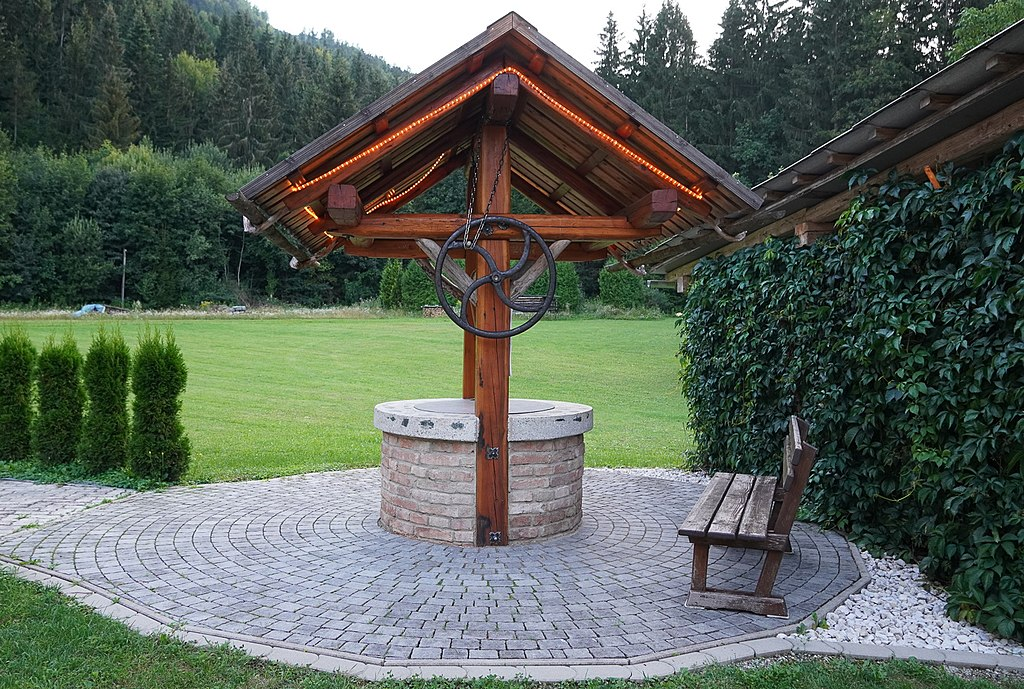
\includegraphics[height=0.32\textheight]{images/Ziehbrunnen.jpg}
	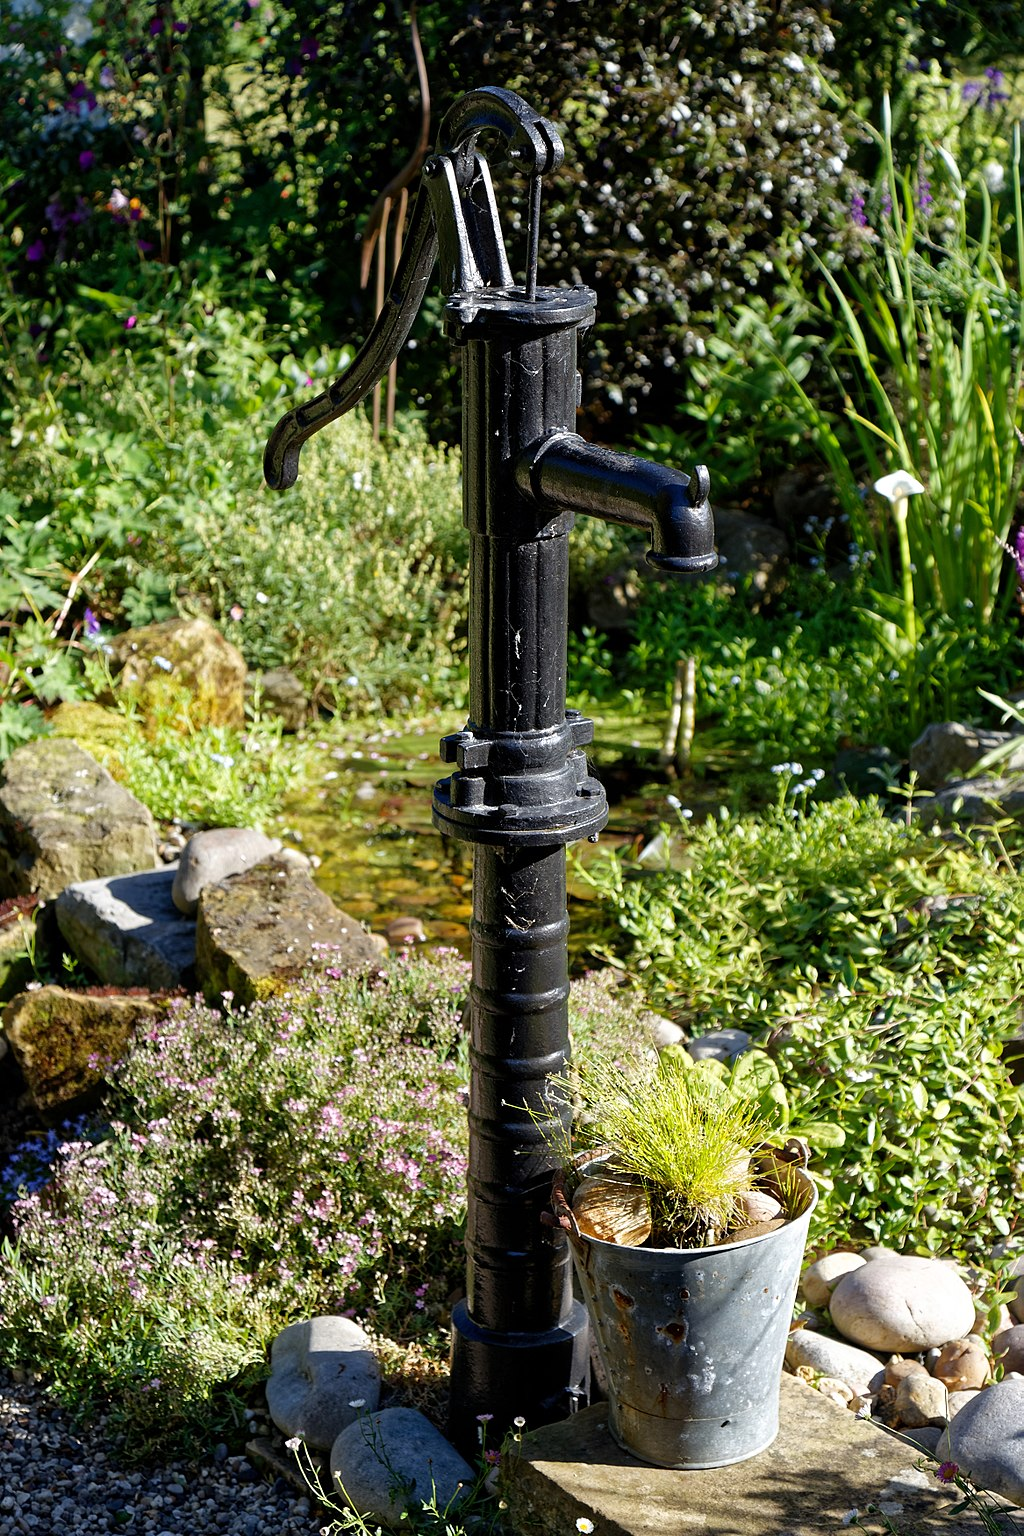
\includegraphics[height=0.32\textheight]{images/Handpumpe.jpg}
	\caption[Bilder von verschiedenen Arten von Brunnen.]{
		Zwei Bilder von verschiedenen Arten von Brunnen.
		Auf der linken Seite ist ein Ziehbrunnen, der heutzutage primär als dekoratives Element verwendet wird.
		Auf der rechten Seite ist ein Brunnen mit Handpumpe, wobei es ähnliche Brunnen auch mit motorisierter Pumpe gibt.
		Dieser Brunnen dient primär als Wasserquelle.\footnotemark
	}
	\label{pic:brunnen}
\end{figure}
\footnotetext{Bildquellen:\\
	Naturpuur, \href{https://creativecommons.org/licenses/by-sa/4.0}{CC BY-SA 4.0}, via Wikimedia Commons\\
	Acabashi, \href{https://creativecommons.org/licenses/by-sa/4.0}{CC BY-SA 4.0}, via Wikimedia Commons
}

Ein Brunnen ist eine Struktur, die Wasser aus einer unterirdischen Quelle verfügbar macht.
Brunnen werden in Gärten oft als dekoratives Element verwendet, können aber auch als Wasserquelle im Garten dienen.
Dabei gibt es verschiedene Arten von Brunnen, wie Ziehbrunnen und Brunnen mit einer Pumpe, wie in \cref{pic:brunnen} zu sehen.
Heutzutage werden Ziehbrunnen primär als dekoratives Element verwendet, während Brunnen mit einer Pumpe als Wasserquelle dienen.
So kann ein Brunnen mit Pumpe in ein automatisches Bewässerungssystem eingebunden werden, wobei auch die gepumpte Wassermenge gemessen werden kann.
Abgesehen davon ist ein Brunnen auch für Frost anfällig, weshalb eine Temperaturmessung helfen kann, Frost zu erkennen und den Brunnen zu schützen.
Auch Wetterdaten können hierfür sinnvoll eingesetzt werden.

\subsubsection{Gartenelement Gartenteich}
\begin{figure}[!htb]
	\centering
	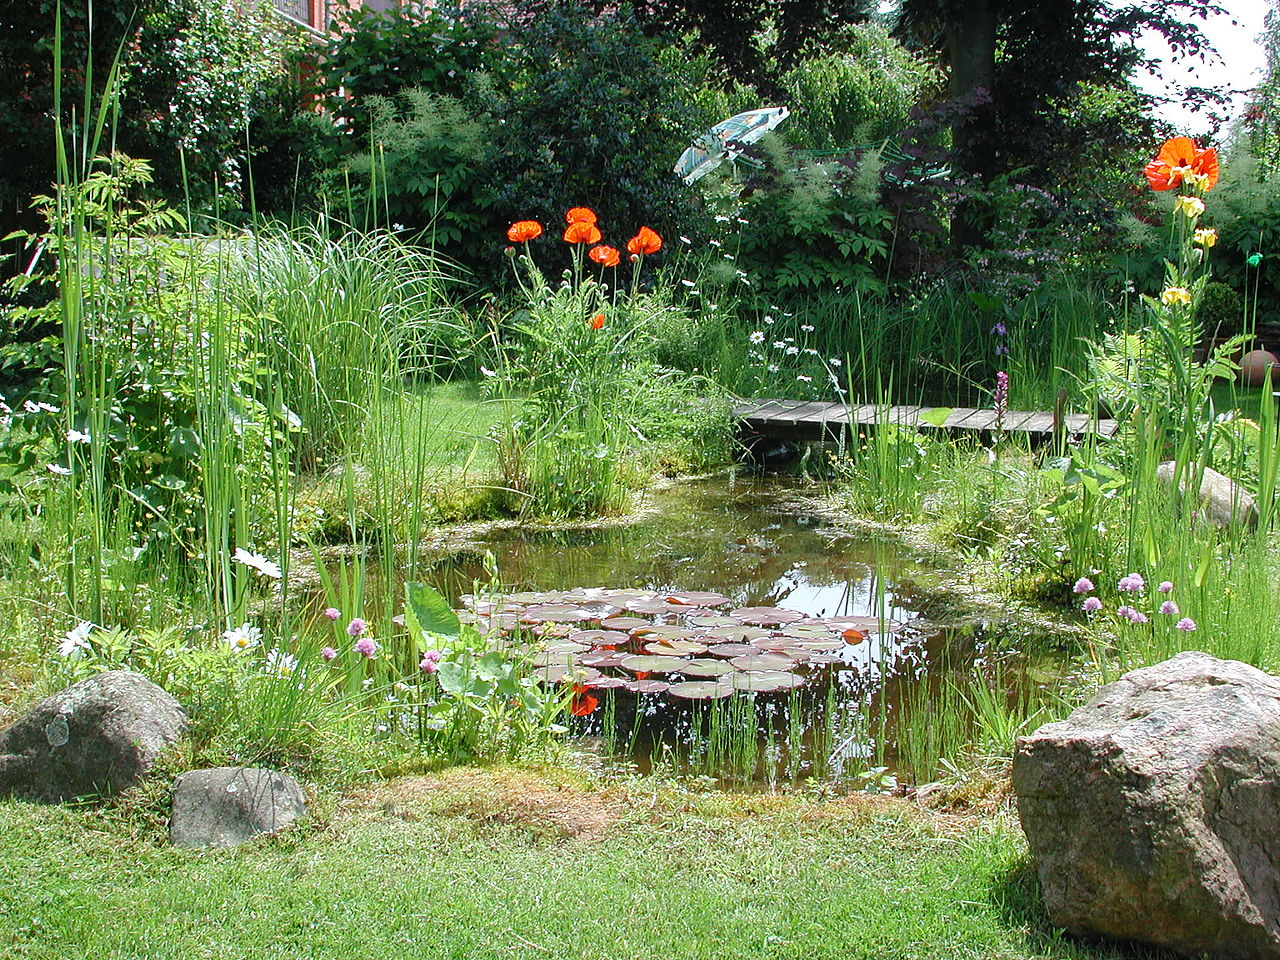
\includegraphics[width=0.5\textwidth]{images/Gartenteich.jpg}
	\caption[Bild eines Gartenteichs.]{
		Bild eines Gartenteichs.
		Der Teich hat eine mittlere Größe und ist mit verschiedenen Pflanzen sowohl am Ufer als auch im Wasser selbst bewachsen.
		Das Wasser ist aufgrund der Menge an Algen grün.\footnotemark
	}
	\label{pic:gartenteich}
\end{figure}

\footnotetext{Bildquelle: Matthias Wilke, \href{https://creativecommons.org/licenses/by-sa/3.0}{CC BY-SA 3.0}, via Wikimedia Commons}

Ein Gartenteich ist ein kleines Gewässer im Garten, welches natürlich oder künstlich angelegt sein kann und in verschiedenen Varianten existiert.
Wie in \cref{pic:gartenteich} zu sehen, kann er beispielsweise von Fischen, Fröschen, Schnecken oder anderen Tieren bewohnt sein, gleichzeitig können auch verschiedene Pflanzenarten im Teich wachsen.
Zur Kontrolle des Wasserspiegels können Pumpen eingesetzt werden.
Ein solcher Teich benötigt regelmäßige Pflege, wie das Entfernen von Algen, das Reinigen des Wassers und das Füttern der Tiere.
Dazu gehört auch die regelmäßige Prüfung der Wasserqualität, um die Gesundheit der Bewohner zu gewährleisten.
Die Wasserqualität setzt sich dabei aus verschiedenen Werten wie der Wasserhärte, dem pH-Wert, dem Sauerstoffgehalt, Nitrit, Nitrat, Ammonium und Ammoniak.
Außerdem fördert ein Überschuss an Nährstoffen das Algenwachstum, was die Wasserqualität verschlechtert und für viele Menschen weniger gut aussieht, wie in \cref{pic:gartenteich} zu sehen.
Wichtig zu beachten sind Wechselwirkungen zwischen den Werten des Teichs, wie zwischen Temperatur und Sauerstoffkonzentration.
So kann Wasser bei niedrigen Temperaturen mehr Sauerstoff lösen.
Auch wichtig ist die Messung des Wasserspiegels, da zu niedriger Wasserspiegel die Pumpe beschädigen und den Tieren und Pflanzen schaden kann~\cite{TeichFische}.
Auf Basis dieser Messung kann der Nutzer benachrichtigt werden, um den Wasserspiegel zu erhöhen.
Auch eine automatische Bewässerung kann hier eingesetzt werden.
Die Fütterung der Tiere kann durch regelbasierte Fütterungssysteme erfolgen.
Diese können die Messwerte der Wasserqualität nutzen, um zu entscheiden, ob und wie viel gefüttert werden soll.
Die Messwerte der Wasserqualität können auch genutzt werden, um automatische Gegenmaßnahmen zu starten.
Dazu gehören unter anderem das Einschalten einer Pumpe oder das Hinzufügen von Chemikalien.

\subsubsection{Gartenelement Pool}
\begin{figure}[!htb]
	\centering
	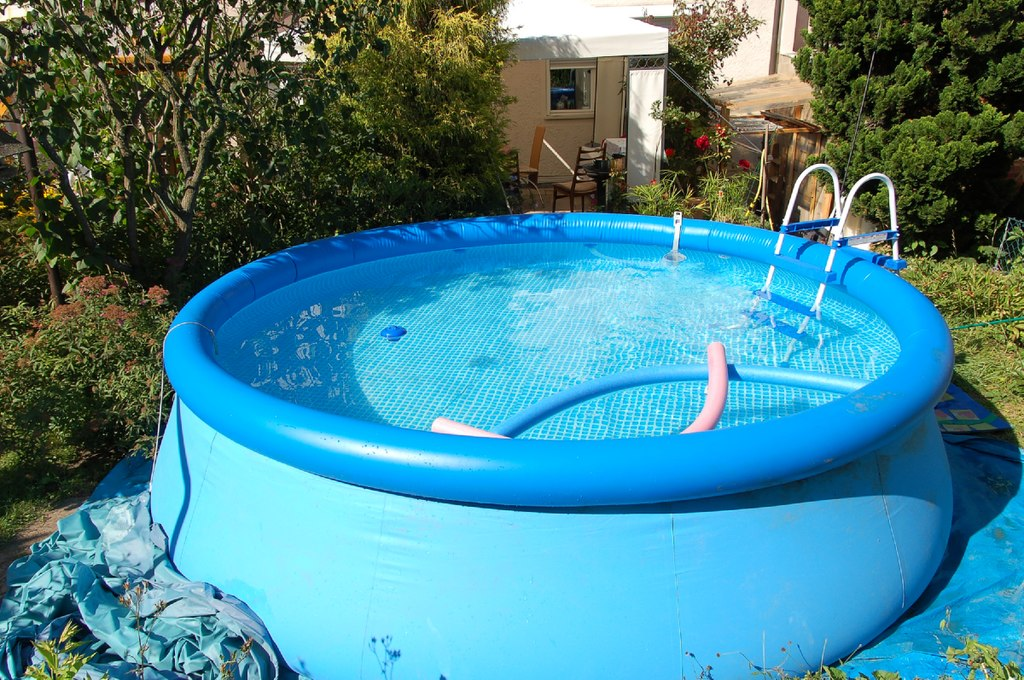
\includegraphics[width=0.5\textwidth]{images/Pool.jpg}
	\caption[Bild eines aufblasbaren Pools in einem Hintergarten.]{
		Bild eines aufblasbaren Pools in einem Hintergarten.
		Der Pool besitzt eine Pumpe zur Reinigung des Wassers und eine Leiter zum Ein- und Aussteigen.\footnotemark
	}
	\label{pic:pool}
\end{figure}

\footnotetext{Bildquelle: Ra Boe, \href{https://creativecommons.org/licenses/by-sa/3.0}{CC BY-SA 3.0}, via Wikimedia Commons}

Ein Pool ist ein künstlich angelegtes Wasserbecken, das zum Schwimmen, Erholen und Spaß haben genutzt wird.
Pools können verschiedene Formen und Größen haben, können im Boden eingelassen oder aufgestellt sein.
Pools benötigen regelmäßige Pflege, um die Wasserqualität zu erhalten.
Wie in \cref{pic:pool} zu sehen, werden dafür selbst in aufblasbaren Pools Pumpen und Filter eingesetzt, um das Wasser zu reinigen.
Diese Filter können aber nicht alle Schadstoffe entfernen, weshalb die Wasserqualität auch durch den Nutzer überwacht werden muss.
Eine gute Wasserqualität ist wichtig für die Gesundheit der Nutzer des Pools.
Aber auch die Technik des Pools kann durch eine schlechte Wasserqualität geschädigt werden.
Zur Wasserqualität gehören Werte wie pH-Wert, Chlor-Wert, Cyansäure-Wert, Redox-Wert und Alkalinität~\cite{PoolWerte}.
Diese Werte müssen regelmäßig überprüft werden, wobei automatische Messsysteme helfen können.
Auch können sich Algen bilden, die die Oberflächen rutschiger machen und somit die Sicherheit gefährden.
Diese können die Werte messen und den Nutzer informieren, wenn die Werte kritisch werden.
Gleichzeitig können automatische Gegenmaßnahmen gestartet werden.
Abgesehen davon ist ein Pool auch für Frost anfällig, weshalb Temperaturmessungen in Kombination mit Wetterdaten helfen können, anbahnenden Frost zu erkennen und den Pool zu schützen.

\subsubsection{Gartenelement Gartenhaus}
\begin{figure}[!htb]
	\centering
	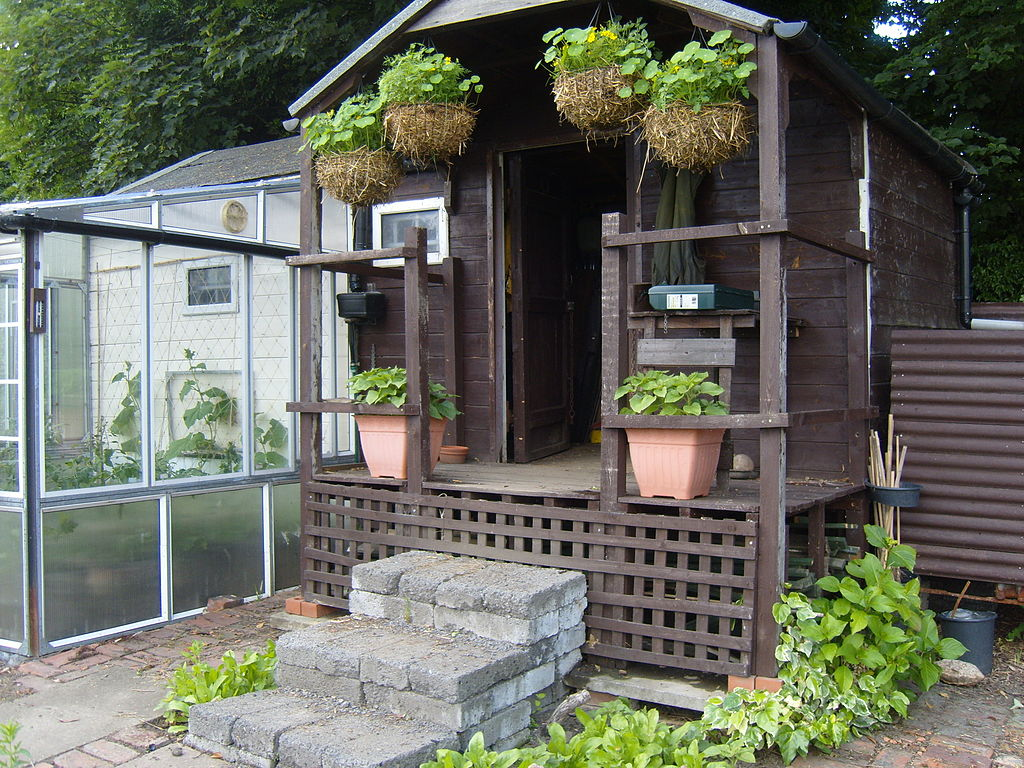
\includegraphics[width=0.5\textwidth]{images/Gartenhaus.jpg}
	\caption[Bild eines Gartenhauses.]{Bild eines Gartenhauses.
		Das Gartenhaus ist frei stehend und mit hängenden Pflanzen beschmückt.\footnotemark
	}
	\label{pic:gartenhaus}
\end{figure}

\footnotetext{Bildquelle: Allotmenteer, \href{https://creativecommons.org/licenses/by-sa/3.0}{CC BY-SA 3.0}, via Wikimedia Commons}

Ein Gartenhaus ist wie in \cref{pic:gartenhaus} zu sehen eine frei stehende Struktur im Garten, welche als Lagerplatz für Gartengeräte, Werkzeuge und andere Utensilien genutzt wird.
Außerdem kann es als Arbeitsbereich für Gartenarbeit, Bastelprojekte oder als Rückzugsort dienen.
Viele Objekte, die in einem Gartenhaus gelagert werden, sind anfällig für Frost und Feuchtigkeit, weshalb Messungen von Temperatur und Luftfeuchtigkeit in einem Gartenhaus sinnvoll sind, wofür auch Wetterdaten hilfreich sein können.
Durch diese Messungen kann der Nutzer informiert werden, wenn die Werte kritisch werden, damit er rechtzeitig Gegenmaßnahmen einleiten kann.
Diese könnten etwa das Heizen des Gartenhauses oder das Entfernen betroffener Gegenstände sein.
Für Gegenstände in der Hütte kann ein intelligentes Regalsystem eingesetzt werden, wofür sich Technologien wie RFID-Tags eignen.
Dadurch kann der Nutzer schnell und einfach Gegenstände finden und verwalten.

\subsubsection{Gartenelement Gehege / Stall}
\begin{figure}[!htb]
	\centering
	\includegraphics[width=0.5\textwidth]{images/Hühnerstall.jpg}
	\caption[Bild eines Hühnerstalls in einem Gehege.]{
		Bild eines Hühnerstalls in einem Gehege.
		Der Stall ist frei stehend und das Gehege ist von einem großen Zaun umgeben.\footnotemark
	}
	\label{pic:stall}
\end{figure}

So wie in \cref{pic:stall} zu sehen ist ein Gehege ein abgegrenzter Bereich im Garten, der der Haltung von Tieren dient und ein Stall ist ein Gebäude, in dem Tiere gehalten werden.
Beide können für die Haltung verschiedener Tiere genutzt werden.
So gibt es Gehege und Ställe für Hühner, Kaninchen, Meerschweinchen, Vögel, Schildkröten und viele andere Tiere.
Diese Tiere benötigen regelmäßige Pflege, wie das Füttern, das Tränken und das Reinigen des Geheges oder Stalls.
Für das Füttern und Tränken können regelbasierte Fütterungssysteme und Tränksysteme eingesetzt werden.
Die Tiere haben außerdem Anforderungen an die Temperatur.
Durch Temperaturmessungen in Kombination mit Wetterdaten kann der Nutzer informiert werden, wenn es zu kalt oder zu warm wird.
So kann der Nutzer rechtzeitig Gegenmaßnahmen einleiten, um die Tiere zu schützen.
Wassernäpfe frieren etwa bei Frost ein, weshalb der Nutzer in diesen Fällen reagieren muss oder eine automatische Wasserenteisung eingesetzt werden kann.
In Ställen kann auch die Luftqualität eine wichtige Rolle spielen, die sich aus CO$_2$-Konzentration und Luftfeuchtigkeit sowie der Temperatur zusammensetzt.
Durch Messungen dieser Werte kann eine automatische Lüftung gesteuert werden.
\footnotetext{Bildquelle: Phil Catterall, \href{https://creativecommons.org/licenses/by-sa/2.0}{CC BY-SA 2.0}, via Wikimedia Commons}

\subsubsection{Gartenelement Bienenstock}
Ein Bienenstock ist eine Struktur, die von Imkern verwendet wird, um Bienen zu züchten und Honig zu produzieren.
Wie in \cref{pic:bienenstock} zu sehen, bestehen Bienenstöcke aus mehreren Elementen, den Bienenkästen, in denen sich Rahmen und Waben befinden.
Diese Bienenkästen haben unterschiedliche Funktionen, wie Brutraum, Honigraum und Futterraum.
Der unterste Kasten hat den Eingang für die Bienen.
Diese Kästen bieten den Bienen Lebensraum und Platz zur Nestbildung und dem Lagern von Honig.

\begin{figure}[!htb]
	\centering
	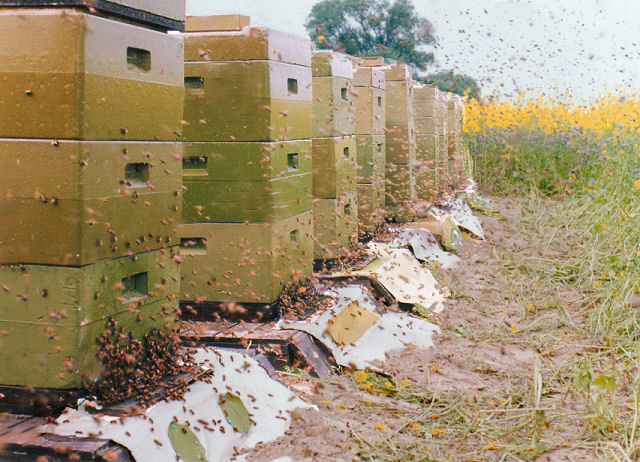
\includegraphics[width=0.5\textwidth]{images/Bienenstock.jpg}
	\caption[Bild mehrerer Bienenstöcke.]{
		Bild mehrerer Bienenstöcke.
		Die Bienen fliegen vor den Bienenstöcken herum.
		Der Eingang für die Bienen befindet sich unten.\footnotemark
	}
	\label{pic:bienenstock}
\end{figure}

\footnotetext{Bildquelle: Axel Hindemith, Public Domain, via Wikimedia Commons}

Bienenstöcke benötigen regelmäßige Pflege, wozu das Füttern, das Überwachen des Bienenstocks und das Ernten des Honigs gehören.
Insbesondere bei der Überwachung des Bienenstocks kann Technik dem Imker helfen.
So kann eine dauerhafte Überwachung des Gewichts des Bienenstocks dem Imker wertvolle Informationen geben~\cite{BienenGewicht}.
Beispielsweise kann ein erhöhter Futterverbrauch am Gewicht abgelesen werden, welcher auf eine Krankheit oder Parasitenbefall hindeuten kann.
Gibt es solche unerwarteten Schwankungen, kann der Imker informiert werden, damit er reagieren kann.
Auch der Futterstand kann damit überwacht werden, da insbesondere im Winter eine Notfütterung nötig werden kann.

Eine weitere wichtige Information für den Imker ist der Status der Bienenkönigin.
Wenn das Volk eine neue Bienenkönigin heranzieht, so zieht die Alte mit einem Teil des Volkes aus, was als Schwärmen bezeichnet wird.
Dies möchte der Imker verhindern, da er dadurch einen Teil seines Volkes verliert.
Auch muss die Bienenkönigin innerhalb der Bienenmasse gefunden werden können.
Wie in \cref{pic:bienenstock} zu sehen, haben die einzelnen Kästen Griffe, die es ermöglichen, die Kästen zu heben.
Die Königin befindet sich in einem dieser Kästen zwischen den Rahmen und anderen Bienen, weshalb die Nutzung von Technik wie RFID-Tags helfen kann, die Königin zu finden.

Die Temperatur im Bienenstock ist ebenfalls ein wichtiger Wert, da der Imker anhand Temperaturänderungen verschiedene Ereignisse im Bienenstock erkennen kann~\cite{BienenTemperatur}.
Auch die Luftfeuchtigkeit ist ein wichtiger Wert für einen Imker, da eine zu niedrige Luftfeuchtigkeit die Brut austrocknen und eine zu hohe Luftfeuchtigkeit den Bienenstock schimmeln lassen kann~\cite{BienenLuftfeuchtigkeit}.

\subsubsection{Gartenelement Kompost}
\begin{figure}[!htb]
	\centering
	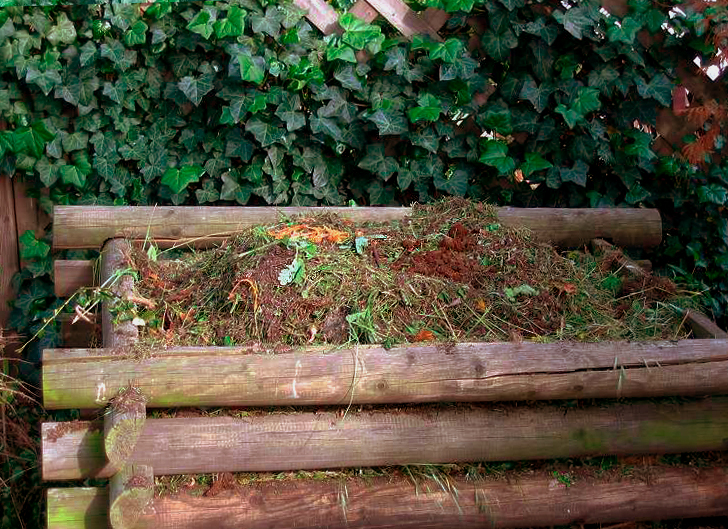
\includegraphics[width=0.5\textwidth]{images/Kompost.jpg}
	\caption[Bild eines Komposthaufens.]{
		Bild eines Komposthaufens.
		Der Kompost besteht aus verschiedenen Elementen, die durch die unterschiedlichen Farben erkennbar sind.\footnotemark
	}
	\label{pic:kompost}
\end{figure}
\footnotetext{Bildquelle: Mussklprozz, \href{https://creativecommons.org/licenses/by-sa/3.0}{CC BY-SA 3.0}, via Wikimedia Commons}
Kompost entsteht durch die Zersetzung von Garten- und Küchenabfällen sowie anderen organischen Materialien wie Laub, Gras und Papierschnipseln.
Das Ergebnis ist ein nährstoffreicher Humus, der als Dünger im Garten eingesetzt werden kann.
Der Prozess der Kompostierung durchläuft dabei mehrere Phasen, nämlich die Vorrotte, Heißrotte, Hauptrotte und Nachrotte.
Gleichzeitig erfordert Kompostierung Aufmerksamkeit und Pflege, um optimale Bedingungen für die Zersetzung zu schaffen.
Diese Bedingungen umfassen die richtige Mischung von grünen (stickstoffreichen) und braunen (kohlenstoffreichen) Materialien, ausreichende Feuchtigkeit und regelmäßige Belüftung~\cite{Kompost}.
Dies ist in \cref{pic:kompost} ersichtlich, wo man den lockeren Komposthaufen mit braunen und grünen Materialien sieht.
Weitergehend unterstützt eine Überwachung der Werte Kohlenstoff, Stickstoff, Feuchtigkeit und ph-Wert den Nutzer bei der Pflege des Kompostes.
Auch die Sicherheit ist ein wichtiger Aspekt, da Kompostierungsprozesse durch die entstehende Wärme zu Bränden führen können.
Außerdem beeinflusst die Temperatur die Belüftungszeiten, die für den Kompostierungsprozess wichtig sind.
Daher ist es wichtig, die Temperatur im Komposthaufen zu überwachen, sodass der Nutzer informiert wird, wenn die Temperatur zu hoch oder zu niedrig ist.
Parameter wie die Temperatur, Zusammensetzung und Feuchtigkeit des Kompostes bestimmen die Geschwindigkeit der Zersetzung und die Qualität des Kompostes.
Daher unterstützt die Überwachung dieser Parameter den Nutzer bei der Pflege des Kompostes.


\subsubsection{Zusammenfassung der Gartenelemente}
Gerade wurde die Vielfalt der verschiedenen Gartenelemente dargestellt
Diese Liste ist nicht vollständig und kann es auch nicht sein, deckt aber die häufigsten Elemente ab.
Andere Elemente können als Unterarten oder Kombinationen dieser Elemente betrachtet werden.
So ist etwa ein Planschbecken ein kleiner Pool ohne Pumpe und Filter oder ein Hochbeet eine Art Beet mit einem erhöhten Bedarf nach Bewässerung.
Alle Gartenelemente können in verschiedenen Arten von Smart Gardening Lösungen profitieren, wobei die Anforderungen an diese unterschiedlich sind.
Hierbei kann es sich beispielsweise um Arbeitserleichterungen, Kosteneinsparungen oder Ertragssteigerungen handeln.
\pagebreak
\begin{table}[!h]
	\centering
	\caption[Gegenüberstellung von Gartenelementen: relevante Messwerte.]{
		Gegenüberstellung verschiedener Gartenelemente basierend auf den relevanten Messwerten.
		In den Zeilen sind die verschiedenen Gartenelemente aufgelistet und in den Spalten die verschiedenen Messwerte.
		Messwerte, die für das jeweilige Gartenelement relevant sind, sind mit einem Häkchen markiert und Messwerte, die nicht relevant sind, mit einem Kreuz.
		Einige Messwerte sind nur für wenige Gartenelemente relevant.
		Diese Elemente sind für die Übersichtlichkeit in der Tabelle als \emph{Andere} enthalten.
		Das betrifft folgende Messwert-Gartenelement-Kombinationen:
		Ammoniumstickstoff und Sauerstoff für Gartenteich, Chlor, Cyansäure, Redox und Alkalinität für Pool, CO$_2$ für Gewächshaus und Gehege/Stall.
		}\label{tab:gartenelementemessungen}
	\begin{tabular}{lllllllllllll}
		\rot[\tabellenwinkel]{				} &
		\rot[\tabellenwinkel]{Temperatur	} &
		\rot[\tabellenwinkel]{Wetter		} &
		\rot[\tabellenwinkel]{Feuchtigkeit	} &
		\rot[\tabellenwinkel]{Schädlinge	} &
		\rot[\tabellenwinkel]{Stickstoff	} &
		\rot[\tabellenwinkel]{Phosphor		} &
		\rot[\tabellenwinkel]{Licht			} &
		\rot[\tabellenwinkel]{Pegel			} &
		\rot[\tabellenwinkel]{Gewicht		} &
		\rot[\tabellenwinkel]{RFID			} &
		\rot[\tabellenwinkel]{pH-Wert		} &
		\rot[\tabellenwinkel]{Andere		}\\\hline
		Rasen					& \OK & \NO & \OK & \OK & \OK & \OK & \NO & \NO & \NO & \NO & \NO & \NO \\
		Beet					& \OK & \OK & \OK & \OK & \OK & \OK & \NO & \NO & \NO & \NO & \NO & \NO \\
		Baum					& \NO & \OK & \OK & \NO & \OK & \NO & \NO & \NO & \NO & \NO & \NO & \NO \\
		Pflanzentopf			& \OK & \OK & \OK & \OK & \OK & \OK & \OK & \NO & \NO & \NO & \NO & \NO \\
		Gewächshaus				& \OK & \OK & \OK & \OK & \OK & \OK & \OK & \NO & \NO & \OK & \NO & \OK \\[.2cm]
		Regentonne				& \OK & \OK & \NO & \NO & \NO & \NO & \NO & \OK & \NO & \NO & \NO & \NO \\
		Brunnen					& \OK & \OK & \NO & \NO & \NO & \NO & \NO & \NO & \OK & \NO & \NO & \NO \\
		Gartenteich				& \OK & \OK & \NO & \OK & \OK & \NO & \NO & \OK & \NO & \NO & \OK & \OK \\
		Pool					& \OK & \OK & \NO & \NO & \NO & \NO & \NO & \NO & \NO & \NO & \OK & \OK \\[.2cm]
		Gartenhaus				& \OK & \OK & \OK & \NO & \NO & \NO & \NO & \NO & \NO & \OK & \NO & \NO \\[.2cm]
		Gehege / Stall			& \OK & \OK & \OK & \NO & \NO & \NO & \NO & \NO & \NO & \NO & \NO & \OK \\
		Bienenstock				& \OK & \NO & \OK & \OK & \NO & \NO & \NO & \NO & \OK & \OK & \NO & \NO \\[.2cm]
		Kompost					& \OK & \NO & \OK & \NO & \OK & \OK & \NO & \NO & \NO & \NO & \OK & \NO \\
	\end{tabular}
\end{table}

Bei den verschiedenen Gartenelementen können unterschiedlichen Messungen sinnvoll eingesetzt werden, wobei die jeweiligen relevanten Messwerte in \cref{tab:gartenelementemessungen} dargestellt sind.
Dabei gibt es einige Gemeinsamkeiten, so profitieren die meisten Gartenelemente von Temperaturmessungen und Wetterdaten.
Weiterhin teilen sich die Gartenelemente, die Pflanzen enthalten, die meisten Messwerte, mit wenigen Ausnahmen.
Dies erklärt sich dadurch, dass Pflanzen ähnliche Bedürfnisse haben und diese Messwerte für die Pflege wichtig sind.
Einige Messwerte sind jedoch nur für wenige der betrachteten Gartenelemente relevant, wie die Pegelmessung und die Gewichtsmessung.

Die für die Gartenelemente relevanten Aktionen sind in \cref{tab:gartenelementeaktuatoren} dargestellt.
Dabei gibt es einige Gemeinsamkeiten, so profitieren alle betrachteten Gartenelemente von der Möglichkeit den Nutzer zu benachrichtigen.
Weiterhin teilen sich die Gartenelemente, die Pflanzen enthalten, die meisten Aktionen, mit wenigen Ausnahmen.
Dies erklärt sich dadurch, dass Pflanzen ähnliche Bedürfnisse haben und diese Aktionen für die Pflege wichtig sind.
Die nicht pflanzenhaltenden Gartenelemente haben dabei sehr unterschiedliche Anforderungen an die Aktionen, wie in der Tabelle ersichtlich.

Aus der kombinierten Betrachtung der Messungen und Aktionen ist ersichtlich, dass ein Fokus auf die pflanzenhaltenden Gartenelemente sinnvoll ist, da diese die meisten Messungen und Aktionen teilen.


\begin{table}[!htb]
	\centering
	\caption[Gegenüberstellung von Gartenelementen: relevanten Aktionen.]{
		Gegenüberstellung verschiedener Gartenelemente basierend auf den relevanten Aktionen des Smart Gardening Systems.
		In den Zeilen sind die verschiedenen Gartenelemente aufgelistet und in den Spalten die verschiedenen Aktionen.
		Aktionen, die für das jeweilige Gartenelement relevant sind, sind mit einem Häkchen markiert und Aktionen, die nicht relevant sind, mit einem Kreuz.
		}\label{tab:gartenelementeaktuatoren}
	\begin{tabular}{llllllllllll}
		\rot[\tabellenwinkel]{						} &
		\rot[\tabellenwinkel]{Benachrichtigung		} &
		\rot[\tabellenwinkel]{Bewässerung			} &
		\rot[\tabellenwinkel]{Düngung				} &
		\rot[\tabellenwinkel]{Schädlinge			} &
		\rot[\tabellenwinkel]{Fütterung				} &
		\rot[\tabellenwinkel]{Tränkung				} &
		\rot[\tabellenwinkel]{Wasserqualität		} &
		\rot[\tabellenwinkel]{Lüftung				} &
		\rot[\tabellenwinkel]{Luftbe-/entfeuchtung	} &
		\rot[\tabellenwinkel]{Heizung				} \\\hline
		Rasen					& \OK & \OK & \OK & \OK & \NO & \NO & \NO & \NO & \NO & \NO \\
		Beet					& \OK & \OK & \OK & \OK & \NO & \NO & \NO & \NO & \NO & \NO \\
		Baum					& \OK & \OK & \NO & \OK & \NO & \NO & \NO & \NO & \NO & \NO \\
		Pflanzentopf			& \OK & \OK & \OK & \OK & \NO & \NO & \NO & \NO & \NO & \NO \\
		Gewächshaus				& \OK & \OK & \OK & \OK & \NO & \NO & \NO & \OK & \OK & \OK \\[.2cm]
		Regentonne				& \OK & \OK & \NO & \NO & \NO & \NO & \NO & \NO & \NO & \NO \\
		Brunnen					& \OK & \OK & \NO & \NO & \NO & \NO & \NO & \NO & \NO & \NO \\
		Gartenteich				& \OK & \NO & \NO & \OK & \OK & \NO & \OK & \NO & \NO & \NO \\
		Pool					& \OK & \NO & \NO & \NO & \NO & \NO & \OK & \NO & \NO & \NO \\[.2cm]
		Gartenhaus				& \OK & \NO & \NO & \NO & \NO & \NO & \NO & \NO & \NO & \NO \\[.2cm]
		Gehege / Stall			& \OK & \NO & \NO & \NO & \OK & \OK & \NO & \OK & \OK & \OK \\
		Bienenstock				& \OK & \NO & \NO & \NO & \NO & \NO & \NO & \NO & \NO & \NO \\[.2cm]
		Kompost					& \OK & \NO & \NO & \NO & \NO & \NO & \NO & \NO & \NO & \NO \\
	\end{tabular}
\end{table}


\subsection{Zusammenfassung Kontext und Umfeld}
In diesem Abschnitt wurden verschiedene Gartenarten und Gartenelemente betrachtet.
Diese weisen unterschiedliche Bedarfe an die Pflege und Überwachung auf, die durch Smart Gardening unterstützt werden können.
Dazu gehören unter anderem automatische Bewässerungs- und Düngesysteme sowie Warnsysteme für Situationen wie Frost oder Schädlinge, in denen der Nutzer eingreifen muss.
Die für ein solches System benötigten Messungen und Aktionen sind unter anderem Temperaturmessungen, Wetterdaten, Feuchtigkeitsmessungen, Schädlingsüberwachung, Bewässerung, Düngung, Fütterung, Tränkung, Überwachung der Wasserqualität, Lüftung, Luftbe- und -entfeuchtung und Heizung.
Daraus folgt, dass ein universelles Sensor- und Aktuatorsystem für Smart Gardening eine Vielzahl von Sensoren und Aktuatoren unterstützen muss.

Gleichzeitig können die Gartenelemente in verschiedenen Kombinationen mit unterschiedlichen Gartenarten auftreten, welche in \cref{tab:gartenelementeartenmapping} dargestellt sind.
Dabei wird ersichtlich, dass einige Gartenarten praktisch alle betrachteten Gartenelemente enthalten können, während andere nur wenige enthalten.
Hierbei ähneln sich der Balkongarten und das Gewächshaus, die jeweils nur drei der betrachteten Elemente enthalten können, während der Kleingarten und Hintergarten jeweils alle der betrachteten Elemente enthalten können.
Auch der Vorgarten und der Landschaftsgarten ähneln sich, was hauptsächlich an dem ähnlichen Zweck der Außenwirkung liegt.

\begin{table}[!htb]
	\centering
	\caption[Kombinationsmöglichkeiten von Gartenarten und Gartenelementen.]{
		Darstellung der verschiedenen Möglichkeiten, Gartenarten und Gartenelemente zu kombinieren.
		In den Zeilen sind die verschiedenen Gartenelemente aufgelistet und in den Spalten die verschiedenen Gartenarten.
		Die Kombinationen, die in der Praxis vorkommen können, sind mit einem Häkchen markiert und die Kombinationen, die nicht vorkommen, mit einem Kreuz.
		}\label{tab:gartenelementeartenmapping}
	\begin{tabular}{lllllllll}
		\rot[\tabellenwinkel]{					} &
		\rot[\tabellenwinkel]{Balkongarten		} &
		\rot[\tabellenwinkel]{Gewächshaus		} &
		\rot[\tabellenwinkel]{Vorgarten			} &
		\rot[\tabellenwinkel]{Kleingarten		} &
		\rot[\tabellenwinkel]{Hintergarten		} &
		\rot[\tabellenwinkel]{Landschaftsgarten	} &
		\rot[\tabellenwinkel]{Landwirtschaft	}\\\hline
		Rasen					& \NO & \NO & \OK & \OK & \OK & \OK & \OK \\
		Beet					& \NO & \NO & \OK & \OK & \OK & \OK & \NO \\
		Baum					& \NO & \NO & \OK & \OK & \OK & \OK & \OK \\
		Pflanzentopf			& \OK & \OK & \OK & \OK & \OK & \NO & \NO \\
		Gewächshaus				& \OK & \OK & \NO & \OK & \OK & \NO & \NO \\[.2cm]
		Regentonne				& \OK & \OK & \OK & \OK & \OK & \NO & \NO \\
		Brunnen					& \NO & \NO & \OK & \OK & \OK & \OK & \OK \\
		Gartenteich				& \NO & \NO & \OK & \OK & \OK & \OK & \NO \\
		Pool					& \NO & \NO & \NO & \OK & \OK & \NO & \NO \\[.2cm]
		Gartenhaus				& \NO & \NO & \NO & \OK & \OK & \NO & \NO \\[.2cm]
		Gehege / Stall			& \NO & \NO & \NO & \OK & \OK & \NO & \OK \\
		Bienenstock				& \NO & \NO & \NO & \OK & \OK & \OK & \OK \\[.2cm]
		Kompost					& \NO & \NO & \OK & \OK & \OK & \NO & \NO \\
	\end{tabular}
\end{table}



\section{Anforderungen}
In diesem Abschnitt werden Anforderungen an ein universelles Sensor- und Aktuatorsystem für Smart Gardening definiert.
Dabei wird auf die Definition von Smart Gardening, die Zielgruppe und die Anwendungsfälle in den Gartenarten und Gartenelementen eingegangen.
Das System soll potenziell alle der oben genannten Anwendungsfälle für die definierte Zielgruppe abdecken können.
Im Folgenden werden dabei zunächst die funktionalen Anforderungen und anschließend die nicht funktionalen Anforderungen betrachtet.


\subsection{Funktionale Anforderungen}
In diesem Abschnitt werden die funktionalen Anforderungen an das System betrachtet, welche beschreiben, was das System leisten soll und was das System benötigt, um diese Leistungen zu erbringen.
In der vorherigen Analyse der Gartenarten und Gartenelemente wurden einige Anforderungen an das System bereits implizit genannt, wie die Notwendigkeit für Sensorik, um Messungen der Umgebung durchzuführen.
In der Analyse wurden bereits einige Messwerte genannt, die für ein Smart Gardening System relevant sind, welche in der \cref{tab:gartenelementemessungen} zusammengefasst sind, wie die Temperatur, die Feuchtigkeit, der Stickstoffgehalt und der pH-Wert.
Diese Liste ist nicht vollständig, sondern deckt nur die häufigsten Nutzungsszenarien ab.
Allein in dieser Auflistung sind bereits 19 Messwerte enthalten, die jeweils nur in bestimmten Szenarien relevant sind.
Die Messung des CO$_2$-Gehalts ist beispielsweise nur im Gewächshaus und im Stall von Interesse.
An dieser Stelle kann die Vielfalt der Sensoren und Sensorschnittstellen nicht abgegrenzt werden, weshalb das System modular sein sollte.
Es sollte möglich sein, Sensoren hinzuzufügen oder zu entfernen.
Da viele Sensoren unterschiedliche Schnittstellen haben, sollten möglichst viele Schnittstellen unterstützt werden, wie I2C, SPI, UART, Modbus und 1-Wire. 

Das System benötigt auch Aktuatorik, um Aktionen durchzuführen.
In der Analyse wurden bereits einige Aktionen genannt, die für ein Smart Gardening System relevant sind, welche in der \cref{tab:gartenelementeaktuatoren} zusammengefasst sind.
Dazu gehören etwa die Bewässerung, die Düngung, die Fütterung und die Tränkung, wobei auch hier einige Aktionen nur in bestimmten Szenarien relevant sind.
Außerdem sieht beispielsweise die Steuerung der Bewässerung für einen Rasen anders aus als für ein Gewächshaus.
Es besteht also ein Bedarf an einer Vielfalt von Aktuatoren, weshalb auch dieser Teil des Systems modular sein sollte.
Es sollte möglich sein, Aktuatoren hinzuzufügen oder zu entfernen.

Weiterhin ist es wichtig, dass das System den Nutzer über wichtige Ereignisse über eine definierbare Schnittstelle wie E-Mail, SMS oder Push-Benachrichtigung benachrichtigen kann.
Dabei soll der Nutzer nicht über jeden kleinen Schritt, sondern nur über besonders wichtige Informationen direkt informiert werden, wozu unter anderem kritische Messwerte oder Aktionen gehören.

Ein weiterer wichtiger Aspekt ist die Möglichkeit der Fernüberwachung.
Regelmäßige Messungen und Aktionen sollen in einem Dashboard zusammengefasst und in einem digitalen Zwilling des Gartens und der Gartenelemente modelliert werden.
Darauf aufbauend wird als weitere Anforderung eine Netzwerkfähigkeit benötigt.
Das System soll in der Lage sein, mit dem Netzwerk zu kommunizieren, wozu die Übertragung der Messwerte, Aktionen und Benachrichtigungen gehört.
Genauer benötigt das System eine LAN und WAN Schnittstelle.

Auch die Konfigurierbarkeit des Systems bezogen auf das Zusammenspiel der Sensoren, Aktuatoren und Benachrichtigungen ist eine wichtige Anforderung.
Diese Konfiguration soll möglichst einfach und intuitiv sein, aber auch komplexere Konfigurationen ermöglichen.
Hierbei ist die grundlegende Möglichkeit der Integration unterschiedlicher Sensoren, Aktuatoren und Benachrichtigungen wichtig.

Aufbauend auf der Konfigurierbarkeit ist die Möglichkeit der Regeldefinition, um das System automatisiert steuern zu können, eine weitere wichtige Anforderung.
So soll es möglich sein, Regeln zu definieren, welche bestimmte Aktionen auslösen können, wenn bestimmte Bedingungen erfüllt sind.
Die Definition folgender Beispielregel soll möglich sein:
\begin{enumerate}
	\item Der Rasen wird bewässert, wenn die Temperatur über 30 Grad steigt.
	\item Der Nutzer wird benachrichtigt.
\end{enumerate}

Ein weiterer wichtiger Aspekt ist die Stromversorgung, da viele Gärten und Gartenelemente existieren, die nicht in der Nähe einer Steckdose liegen.
Daher muss das System in solchen Fällen autonom arbeiten können, was beispielsweise durch Solarzellen oder Akkus erfolgen kann.
Gleichzeitig soll das System in diesem autonomen Zustand möglichst selten aufgeladen werden müssen, weshalb ein geringer Energieverbrauch wichtig ist.
Auch eine fest installierte Wasserversorgung ist nicht immer gegeben.
Daher sollte das System auch mit einer Regentonne oder einem Brunnen arbeiten können.

Zusammengefasst soll das System den folgenden funktionalen Anforderungen genügen, die hierbei nach ihrer Wichtigkeit sortiert sind:
\begin{itemize}
	\item Messung mittels Sensoren
	\item Konfiguration des Systems
	\item Regeldefinition
	\item Dashboard mit digitalem Zwilling basierend auf den Messwerten und Aktionen
	\item Steuerung von Aktuatoren
	\item Autonomer Betrieb
	\item Benachrichtigung des Nutzers
\end{itemize}
Diese Reihenfolge ergibt sich aus der Annahme, dass die Messung der Umgebung die Grundlage für alle weiteren Funktionen bildet.
Die Konfiguration des Systems ist wichtig, um das System an die individuellen Bedürfnisse des Nutzers anzupassen und daran anschließend die Regeldefinition, um das System automatisiert steuern zu können.
Ein Dashboard mit digitalem Zwilling ist wichtig, um dem Nutzer einen Überblick über den Zustand des Gartens zu geben.
Die Steuerung von Aktuatoren ist in der Priorität hinter der Sensorik, da die Sensorik die Grundlage für die Steuerung bildet und viele Anwendungsfälle ohne Aktuatoren auskommen können.
Der autonome Betrieb ist wichtig, um das System auch in Gärten ohne Strom- und Wasserversorgung einsetzen zu können und eine Benachrichtigung des Nutzers ist wichtig, um den Nutzer über wichtige Ereignisse zu informieren.



\subsection{Nicht funktionale Anforderungen}
In diesem Abschnitt werden die nicht funktionalen Anforderungen an das System betrachtet, welche beschreiben, wie das System arbeiten soll.
Dabei sind die nicht funktionalen Anforderungen nach ihrer Wichtigkeit sortiert.

An erster Stelle steht der Preis des Systems.
Da die primäre Zielgruppe Hobbygärtner und somit Privatpersonen mit begrenztem Budget sind, sollte das System möglichst günstig sein.
Auch der Energieverbrauch und die Wartung des Systems sind Faktoren, die den Preis beeinflussen.

Weiterer wichtiger Punkt ist der Schutz beziehungsweise die Resilienz des Systems vor den Elementen.
Das System muss wasserfest, dreckfest, robust und temperaturbeständig sein, sowie fest installierbar, damit es nicht vom Wind weggeweht werden kann.
Für den Wasser- und Staubschutz gibt es die IP Schutzart, wobei für einen universellen Einsatz im Garten IP Schutzklasse 6 staubdicht und Schutzgrad 8 geschützt vor andauerndem Untertauchen, also IP68 sinnvoll ist.
Auch die Sonne mit ihren UV-Strahlen kann dem System schaden, weshalb es vor der Sonne geschützt werden muss~\cite{LichtPlastik,LichtPlastik2}.

Auch die Bedienung des Systems soll nutzerfreundlich sein.
Der Nutzer soll nicht lange brauchen, um das System zu bedienen, es sollte also eine flache Lernkurve haben.
Dies ist insbesondere wichtig, da vor allem Hobbygärtner das System nutzen werden.

Ein weiterer wichtiger Aspekt ist die Sicherheit des Systems.
Das Smart Gardening System ist mit Sensorik ausgestattet, welche Daten über den Garten und Umgebung erheben.
Kommt ein Angreifer in Besitz dieser Daten, können sie potenziell ausgenutzt werden.
Sie können beispielsweise genutzt werden, um das Verhalten der Bewohner zu analysieren, in das Haus einzubrechen oder den Garten zu zerstören.
Da die Messdaten oder Auswertungen dieser Messdaten über ein Netzwerk übertragen werden, ist eine sichere Übertragung wichtig, beispielsweise durch Verschlüsselung der Daten.
Weiter dürfen die Daten bei der Übertragung nicht geändert werden, die Datenintegrität muss also gewährleistet sein.
Des Weiteren ist auch ein Angriff auf die Aktuatorik denkbar.
Ein Angreifer könnte etwa die Bewässerung des Gartens manipulieren, wenn das System eine Fernsteuerung zulässt.
Daher darf die Aktuatorik nur von authentifizierten Nutzern gesteuert werden.
Das Gleiche gilt auch, wenn das Smart Gardening System von Landwirten oder Gärtnern eingesetzt wird.

Ein sparsamer Energieverbrauch ist aus zwei Gründen wichtig.
Zum einen hat der Energieverbrauch einen Einfluss auf den Preis des Systems, da ein höherer Energieverbrauch auch höhere Betriebskosten bedeutet.
Zum anderen ist ein sparsamer Energieverbrauch wichtig, wenn das System auch unabhängig vom Stromnetz betrieben werden können soll.

Auch die Verfügbarkeit des Systems ist wichtig, da ein unerkannter Ausfall des Systems zu Schäden im Garten führen kann.
Da die Verfügbarkeit nicht garantiert werden kann, muss der Nutzer im Fehlerfall informiert werden.

Die Wartbarkeit des Systems ist ein weiterer wichtiger Aspekt.
Das System soll möglichst einfach wartbar sein, damit der Nutzer es selbst warten kann.
Dazu gehört beispielsweise, dass das System modular aufgebaut ist, sodass defekte Sensoren oder Aktuatoren einfach ausgetauscht werden können.

Weiterhin soll das System möglichst unauffällig sein, was insbesondere für Vorgärten wichtig ist, die von der Straße aus einsehbar sind.
Dazu gehört, dass es nicht zu groß ist und sich in die Umgebung integrieren lässt.

Zusammengefasst soll das System diesen nicht funktionalen Anforderungen genügen:
\begin{itemize}
	\item Preis
	\item Schutz vor den Elementen
	\item Nutzerfreundliche Bedienung
	\item Sicherheit (Datenintegrität, Datenschutz, Angriffssicherheit)
	\item Sparsamer Energieverbrauch
	\item Verfügbarkeit des Systems
	\item Einfache Wartbarkeit
	\item Visuelle Unauffälligkeit
\end{itemize}

\subsection{Zusammenfassung der Anforderungen}
In diesem Abschnitt wurden die funktionalen und nicht funktionalen Anforderungen an ein universelles Sensor- und Aktuatorsystem für Smart Gardening definiert.
Diese Anforderungen wurden auf Basis der Definition von Smart Gardening, der Zielgruppe und der Anwendungsfälle in den Gartenarten und Gartenelementen erarbeitet.

Die funktionalen Anforderungen beschreiben, was das System leisten soll und was das System benötigt, um diese Leistungen zu erbringen.
Dabei wurden die Messung mittels Sensoren, die Steuerung von Aktuatoren, die Benachrichtigung des Nutzers, die Konfiguration des Systems, die Regeldefinition, ein Dashboard mit digitalem Zwilling basierend auf den Messwerten und Aktionen und der autonome Betrieb als funktionalen Anforderungen definiert.

Die nicht funktionalen Anforderungen beschreiben, wie das System arbeiten soll.
Dabei wurden die Sicherheit, die Verfügbarkeit des Systems, der Preis, der sparsame Energieverbrauch, die einfache Wartbarkeit, der Schutz vor den Elementen, die visuelle Unauffälligkeit und die nutzerfreundliche Bedienung als nicht funktionale Anforderungen definiert.



\section{Zusammenfassung der Analyse}
In diesem Kapitel wurde der Einsatz von Smart Gardening im Garten analysiert.
Die Zielgruppe besteht vorrangig aus Gärtnern, unterteilt in Hobbygärtner und professionelle Gärtner sowie nachrangig Landwirte.
Smart Gardening kann in verschiedenen Gartenarten und Gartenelementen eingesetzt werden.
Dabei wurden die Gartenarten Balkongarten, Gewächshaus, Vorgarten, Kleingarten, Hintergarten, Landschaftsgarten und zusätzlich die Landwirtschaft betrachtet.
Hier können Smart Gardening Lösungen etwa Arbeitserleichterungen, Kosteneinsparungen oder Ertragssteigerungen bringen.
Gleichzeitig stellen die Strom-, Wasser- und Internetversorgung für das Smart Gardening System eine Herausforderung dar.
Als Gartenelemente wurden Rasen, Beet, Baum, Pflanzentopf, Gewächshaus, Regentonne, Brunnen, Gartenteich, Pool, Gartenhaus, Gehege/Stall, Bienenstock und Kompost betrachtet.

Darauf aufbauend wurden Anforderungen an ein universelles Sensor- und Aktuatorsystem für Smart Gardening definiert.
Zu den funktionalen Anforderungen gehören die Messung mittels Sensoren, die Steuerung von Aktuatoren, die Benachrichtigung des Nutzers, die Konfiguration des Systems, die Regeldefinition, ein Dashboard mit digitalem Zwilling basierend auf den Messwerten und Aktionen und der autonome Betrieb.
Zu den nicht funktionalen Anforderungen gehören die Sicherheit, die Verfügbarkeit des Systems, der Preis, der sparsame Energieverbrauch, die einfache Wartbarkeit, der Schutz vor den Elementen, die visuelle Unauffälligkeit und die nutzerfreundliche Bedienung.
Basierend auf diesen Anforderungen wird im nächsten Kapitel der Stand der Technik betrachtet, um zu sehen, inwieweit existierende Systeme diesen Anforderungen genügen.
	% !TEX root = ../thesis.tex
\chapter{Stand der Technik}\label{ch:stand-der-technik}
In diesem Kapitel wird der Stand der Technik im Bereich der Sensor- und Aktuatorsysteme untersucht.
Dazu werden verschiedene Konzepte und Beispielsysteme vorgestellt, die für ähnliche oder vermeintlich ähnliche Anwendungsfälle konzipiert wurden und eingesetzt werden.
Diese Konzepte und Beispiele werden dann mit den Anwendungsfällen und Anforderungen an das angestrebte universelle Sensor- und Aktuatorsystem für Smart Gardening verglichen.
Dabei werden deutlich die Unterschiede herausgearbeitet und erläutert, warum die Systeme für ein universelles Sensor- und Aktuatorsystem für Smart Gardening geeignet oder ungeeignet sind.
Bei diesen Beispielen handelt es sich sowohl um kommerzielle Produkte als auch um wissenschaftliche Arbeiten.
Zunächst werden IoT-Sensoren und Gateways vorgestellt, dann wird auf Messkoffer eingegangen, darauf folgen Sensor-Hubs und Industrial Remote Monitoring (and Control).
Anschließend werden die verschiedenen Systeme gegenübergestellt und anhand der Anforderungen bewertet.
Zum Schluss werden die Ergebnisse zusammengefasst, inwiefern die existierenden Systeme die Anforderungen erfüllen und inwiefern sie als Grundlage für das angestrebte System dienen können.



\section{IoT-Sensoren}
\begin{figure}[!htb]
	\centering
	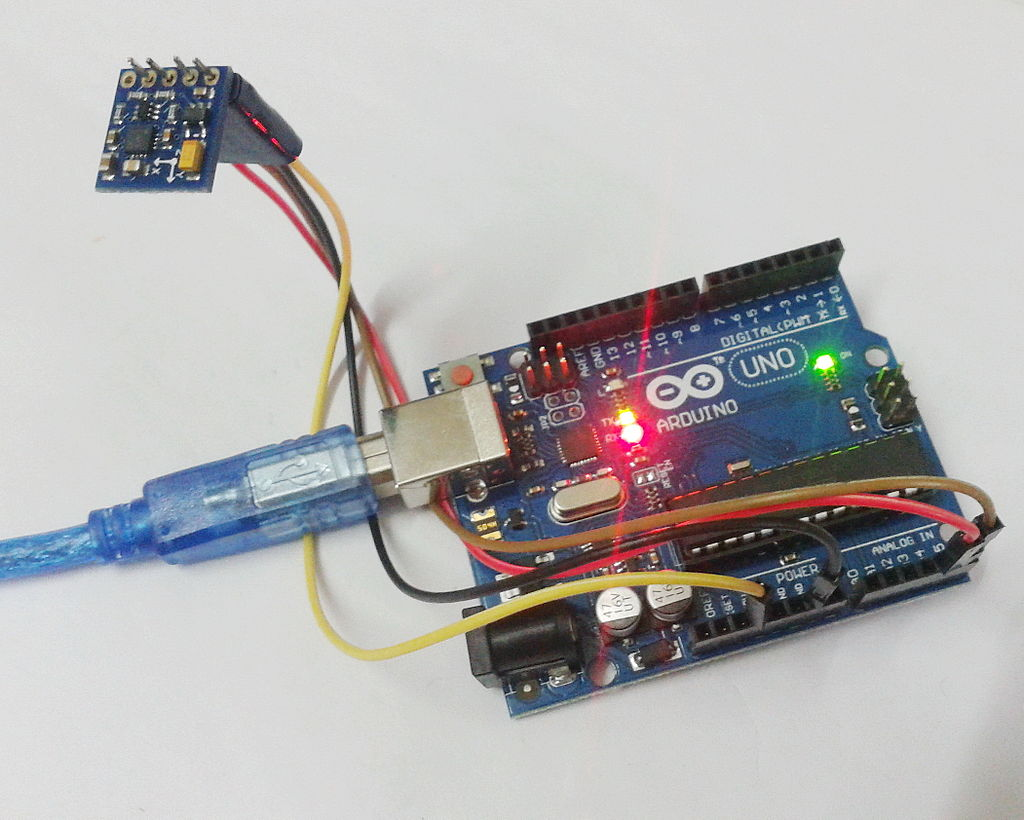
\includegraphics[height=0.4\textheight]{images/IoT-Sensor.jpg}
	\caption[Bild eines IoT-Sensors.]{Bild eines IoT-Sensors.
		Dieser besteht aus dem Mikrocontroller Arduino Uno, welcher die Steuerung übernimmt, und einem Gyroskop als Sensor, welcher an den Mikrocontroller angeschlossen ist.
		Er weist einige Schnittstellen wie Pins, USB und WLAN auf.\footnotemark
	}
	\label{pic:iotsensor}
\end{figure}

Als IoT-Sensoren werden autonome, netzwerkfähige Sensoren bezeichnet, wie in \cref{pic:iotsensor} zu sehen~\cite{IoTSensor}.
Ihr Aufbau ist, wie in der Abbildung zu sehen, simpel und besteht meist aus einem Mikrocontroller, der die Steuerung übernimmt, einem Sensor, der die Messung durchführt, einer Stromversorgung sowie einer Kommunikationsschnittstelle.
Es gibt verschiedene Arten von IoT-Sensoren, die in unterschiedlichen Bereichen wie der Industrie, der Landwirtschaft oder dem Garten eingesetzt werden.
Der Markt für IoT wächst stetig und es kommen immer neue Sensoren auf den Markt~\cite{IoTSensorenAbsatz}.

IoT-Sensoren können verschiedene Parameter messen, wie Temperatur, Luftfeuchtigkeit oder Bewegung.
Sie sind in der Lage, die gemessenen Daten an eine zentrale Stelle zu senden, wo sie ausgewertet werden können.
Dadurch können sie beispielsweise zur Überwachung bestimmter Parameter eingesetzt werden, wobei ein einzelner Sensor dabei meist nur einen Parameter misst.
Es gibt jedoch auch Sensoren, die mehrere Parameter messen können und dementsprechend flexibler einsetzbar sind.

IoT-Sensoren können sowohl fest installiert als auch mobil sein und außerdem können sie autonom arbeiten und benötigen keine manuelle Bedienung.
Dadurch können sie beispielsweise in schwer zugänglichen Bereichen eingesetzt werden.
Sie sind normalerweise stromsparend und können über lange Zeiträume betrieben werden, wodurch sie sich auch für den Einsatz in abgelegenen Gebieten eignen.
Außerdem sind sie meist kostengünstig und können in großen Stückzahlen eingesetzt werden.
Wie in \cref{pic:iotsensor} zu sehen, sind IoT-Sensoren einfach aufgebaut und können auch von Laien gebaut werden.

Gleichzeitig erfüllen die IoT-Sensoren allein nicht die Anforderungen an eine Automatisierung von Prozessen.
Sie können aber als Grundlage oder als Teil eines solchen Systems dienen und dabei die Rolle der Sensorik, nicht aber der Aktuatorik und Steuerung übernehmen.
Dies bietet einige Vorteile im Vergleich zu herkömmlichen Sensoren.
So müssen für eine größere Fläche keine Kabel durch den ganzen Garten gelegt werden, um Sensoren zu verbinden und gleichzeitig ist der Umbau leichter.
Auch wird durch die Autonomie der einzelnen Sensoren ein einzelner Ausfallpunkt umgangen.
Gleichzeitig ergeben sich einige Nachteile im Vergleich zu einfachen Sensoren, wie mehr Ausfallmöglichkeiten aufgrund der höheren Komplexität.
Außerdem sind die Kosten höher, da jeder Sensor einen eigenen Mikrocontroller, eine eigene Stromversorgung und Kommunikationsschnittstelle benötigt.
Zusammengefasst können IoT-Sensoren als Teil eines universellen Sensor- und Aktuatorsystems für Smart Gardening eingesetzt werden, indem sie die Rolle einiger Sensoren einnehmen, sie sind aber kein Ersatz für das Gesamtsystem.
\footnotetext{Bildquelle: Rahat, \href{https://creativecommons.org/licenses/by/4.0}{CC BY 4.0}, via Wikimedia Commons}



\section{Gateway}
\begin{figure}[!htb]
	\centering
	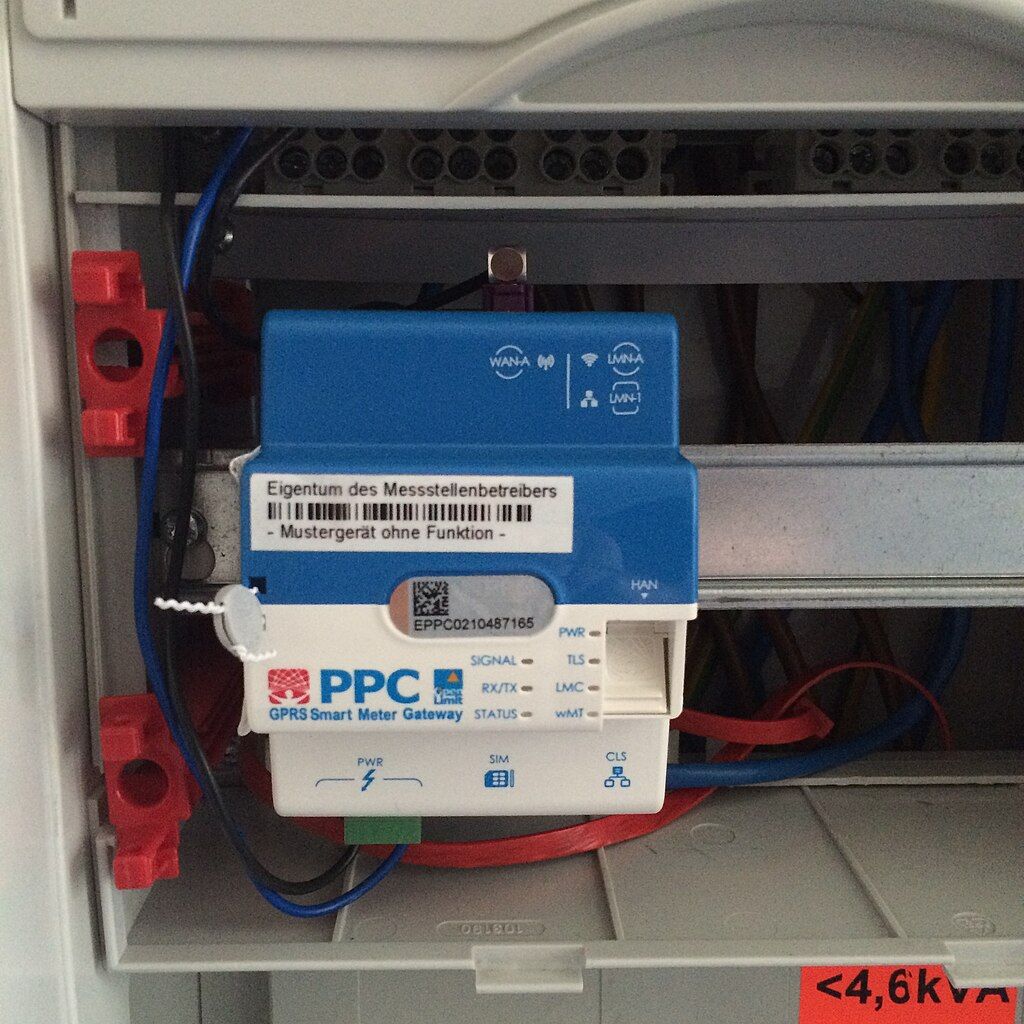
\includegraphics[height=0.4\textheight]{images/Gateway.jpg}
	\caption[Bild eines Smart-Meter-Gateways]{
		Bild eines Smart-Meter-Gateways, welches als Gateway für das lokale metrologische Netzwerk, ein Netz aus elektronischen Zählern wie Strom, Wasser, Gas und Wärme zu einem WAN und einem HAN dient~\cite{SmartMeterGateway}.\footnotemark
	}
	\label{pic:gateway}
\end{figure}
\footnotetext{Bildquelle: Pichiciago, \href{https://creativecommons.org/licenses/by-sa/4.0}{CC BY-SA 4.0}, via Wikimedia Commons}
In diesem Kontext bezeichnet ein Gateway eine Technologie, mit der Geräte ohne Internetfähigkeit internetfähig gemacht werden können.
Gateways können beispielsweise für Industrieanlagen, Sensoren oder Aktuatorik eingesetzt werden und haben häufig die Form einer kleinen Box wie in \cref{pic:gateway} zu sehen.
Auch Sensornetze, also Verbunde aus untereinander kommunizierenden Sensorknoten, können über ein Gateway an das Internet angeschlossen werden.
Häufig sind in solchen Anlagen Schnittstellen für beispielsweise Modbus verfügbar, an die das Gateway angeschlossen werden kann.
So ist ein Zugriff auf Daten sowie einer Steuerung über das Netzwerk möglich, was ohne Gateway nur vor Ort möglich wäre.
Auch einfache Sensoren können auf diese Art ihre Daten dem Netzwerk zur Verfügung stellen.

Als rein unterstützende Technologie können Gateways den definierten Anforderungen nicht entsprechen, da sie weder die Sensorik noch die Aktuatorik darstellen.
Sie können dennoch ein wichtiger Bestandteil eines solchen Systems sein, da sie die Integration von Sensoren und Aktuatoren in das Netzwerk ermöglichen.
So können etwa einfache Sensoren zu IoT-Sensoren aufgerüstet und Aktuatorik internetfähig gemacht werden, was eine Flexibilität im Aufbau des Systems ermöglicht.

Zusammengefasst können Gateways ein Bestandteil eines universellen Sensor- und Aktuatorsystems für Smart Gardening darstellen, indem sie Sensoren oder Aktuatoren an das System anschließen.
Sie sind jedoch nur unterstützende Technologie und können die Anforderungen nicht erfüllen.



\section{Messkoffer}
Als Messkoffer werden simple Koffer bezeichnet, die verschiedene Messgeräte enthalten.
Dabei kann es sich um einfache Multimeter, aber auch um komplexere Geräte handeln.
Meist sind diese Koffer beim Verkauf mit einer bestimmten Auswahl an Geräten bestückt, die von Handwerkern oder Technikern verwendet werden, um verschiedene Messungen durchzuführen.
Solche Messkoffer existieren auch für den Gartenbereich und können den Gärtner mobil bei der Arbeit unterstützen.
Sie sind jedoch nicht autonom, sondern müssen vom Nutzer bedient und die anfallenden Daten müssen durch den Nutzer manuell ausgewertet werden.
Auch Benachrichtigungen bei bestimmten Ereignissen wie bestimmten Temperaturschwellenwerten sind nicht möglich.
Aus diesen Gründen sind sie nicht für die Automatisierung von Prozessen geeignet.

\begin{figure}[!htb]
	\centering
	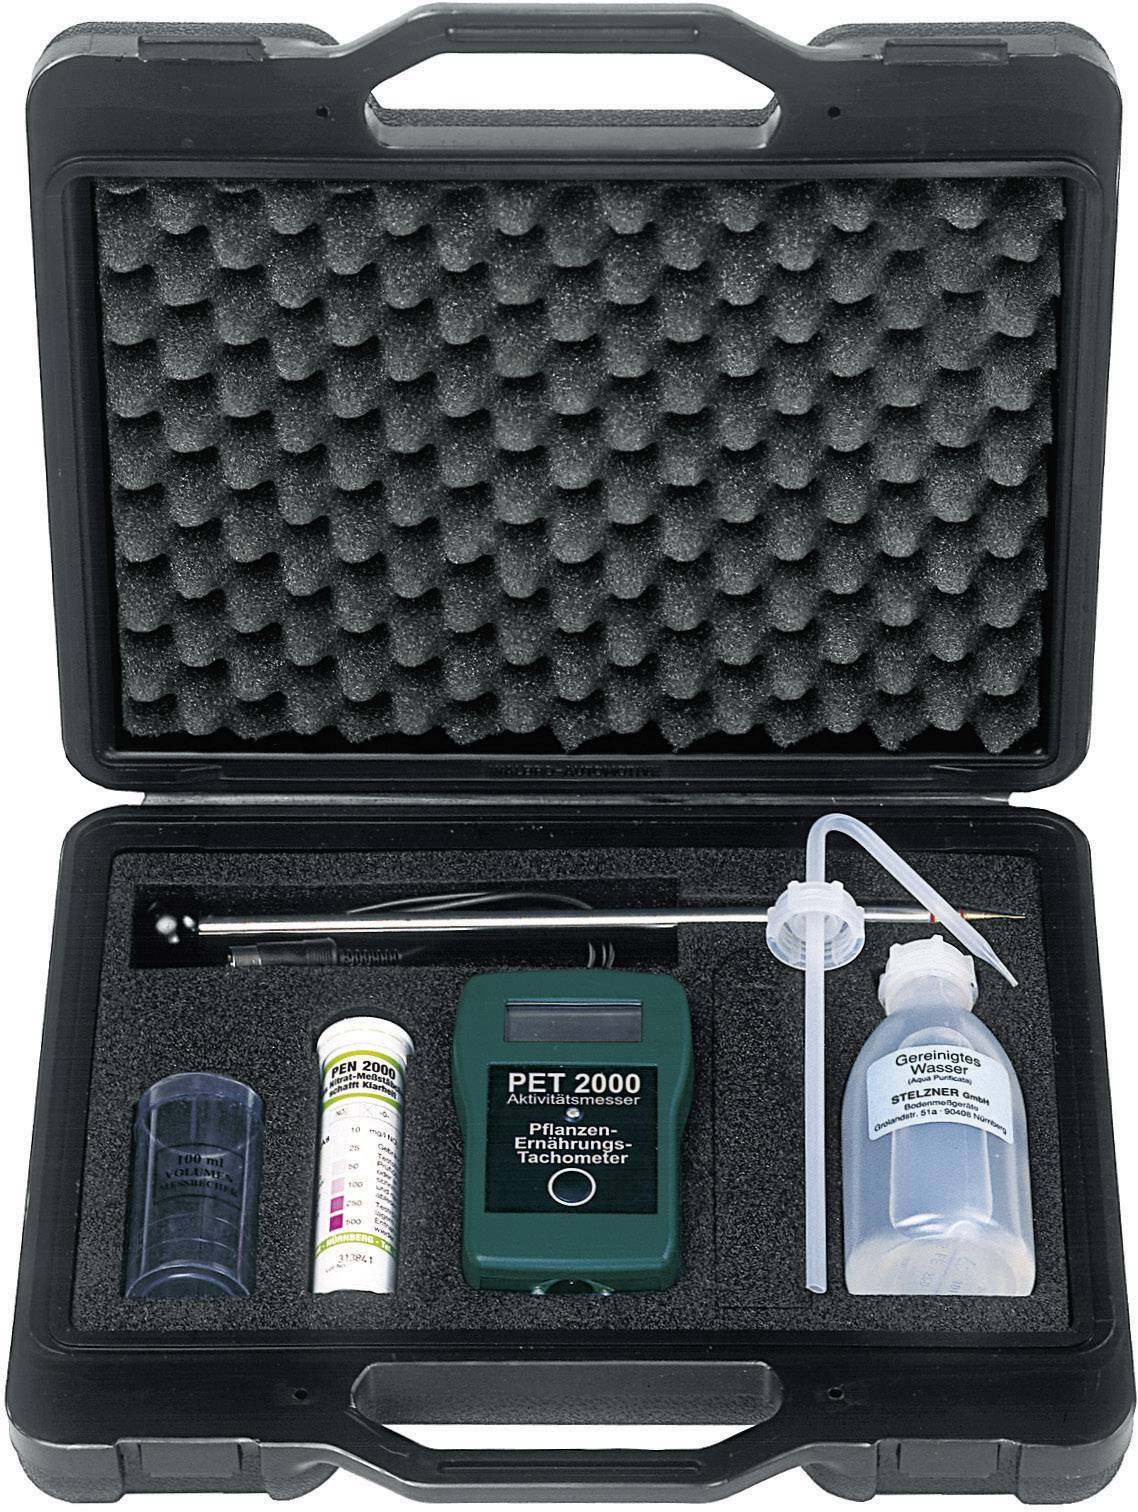
\includegraphics[width=0.4\textwidth]{images/Messkoffer.jpg}
	\caption[Bild eines Stelzner Aktivitätsmesskoffer PET 2000.]{
		Bild eines Stelzner Aktivitätsmesskoffer PET 2000.
		Dieser beinhaltet unter anderem einen Aktivitätsmesser PET 2000, Nitrat-Messstäbchen, Behälter und eine Flasche mit entinonisiertem Wasser.\footnotemark}
	\label{pic:messkoffer}
\end{figure}

\footnotetext{\href{https://asset.conrad.com/media10/isa/160267/c1/-/de/101879_BB_00_FB/image.jpg}{Bildquelle: Stelzner Aktivitätsmesskoffer PET 2000}}

Ein Beispiel dafür ist der Stelzner Aktivitätsmesskoffer PET 2000~\cite{Stelzner}, dessen Einsatzgebiet hauptsächlich der Gartenbau ist.
Dieser Koffer enthält, wie in \cref{pic:messkoffer} zu sehen, das Messgerät PET 2000 zur Bestimmung der im Boden gelösten Nährsalze, sowie Nitratmessstäbchen und weitere unterstützende Materialien.
Auf Basis dieser Messungen kann der Gärtner entscheiden, ob und wie gedüngt werden muss.
Somit deckt der Koffer einen Anwendungsfall ab, nämlich die Düngung.
Da aber sowohl Messung als auch Entscheidung über die Düngung manuell durch den Gärtner durchgeführt werden muss, decken solche Messkoffer die Anforderungen nicht ab.
Zusammengefasst sind Messkoffer nur teilweise Smart Gardening geeignet, da sie den Gärtner zwar in bestimmten Aufgaben unterstützen, jedoch keine Automatisierung von Messungen und Prozessen ermöglichen.




\section{Sensor-Hub}
Ein Sensor-Hub ist ein Gerät, das verschiedene Anschlüsse aufweist und somit mit unterschiedlichen Sensoren und Geräten verbunden werden kann.
Es kann sowohl mobil und somit an vielen Orten einsetzbar sein als auch fest installierbar.
Gleichzeitig ist es autonom, sodass es auch ohne manuelle Bedienung arbeiten kann.
Diese Technologie kann in verschiedenen Bereichen eingesetzt werden, wie in der Industrie, der Landwirtschaft oder im Gartenbau.
Dabei kann es sowohl für einfache Messungen als auch für komplexere Messungen eingesetzt werden, wobei komplex bedeutet, dass mehrere Messungen zu einem neuen Wert kombiniert werden.
Das kann etwa die Kombination von Temperatur und Luftfeuchtigkeit sein, um den Belüftungsbedarf eines Raumes zu bestimmen oder die Kombination von mehreren Pegelmessungen in einer Regentonne, um die Restdauer der Bewässerung zu bestimmen.

\subsection{Universal Wireless Sensor Node}

\begin{figure}[!htb]
	\centering
	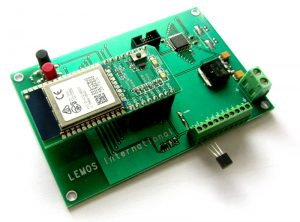
\includegraphics[width=0.5\textwidth]{images/UniversalWirelessSensorNode.jpg}
	\caption[Bild eines Universal Wireless Sensor Node.]{Bild eines Universal Wireless Sensor Node.\footnotemark}
	\label{pic:universal-sensor-node}
\end{figure}

\footnotetext{Bildquelle: \href{https://lemosint.com/wp-content/uploads/2019/04/UniversalWirelessSensorNode-300x222.jpg}{Universal Wireless Sensor Node}}

Der Universal Wireless Sensor Node von Lemos International Company Inc., wie in \cref{pic:universal-sensor-node} dargestellt~\cite{Universal}, basiert auf einem fortschrittlichen Mikrocontroller und ist in der Lage, eine Vielzahl von Sensoren für unterschiedliche Anwendungen zu integrieren.
Es unterstützt die Erfassung von Daten wie Temperatur, Luftfeuchtigkeit, Bewegungen und gefährlichen Gasen.
Dafür verfügt es über einige Protokolle zur Kommunikation, darunter I2C, SPI und asynchrone Protokolle.
Der Sensor Node kann mit verschiedenen Funkmodulen betrieben werden, die in energiesparenden, lizenzfreien Frequenzbereichen wie 433 MHz, 915 MHz und 2.4 GHz und dem amerikanischen Multi-Use Radio Service arbeiten.
Diese Flexibilität ermöglicht den Einsatz in zahlreichen Mess- und Steuerungsaufgaben, die für Smart Gardening relevant sind.
Gleichzeitig erfüllt der Universal Wireless Sensor Node die Anforderungen an ein universelles Sensor- und Aktuatorsystem für Smart Gardening nur teilweise.
Er kann zwar eine Vielzahl von Sensoren integrieren und die Daten an eine zentrale Stelle senden, jedoch fehlt die Aktuatorik und Steuerung.

\subsection{Loggito Logger}

\begin{figure}[!htb]
	\centering
	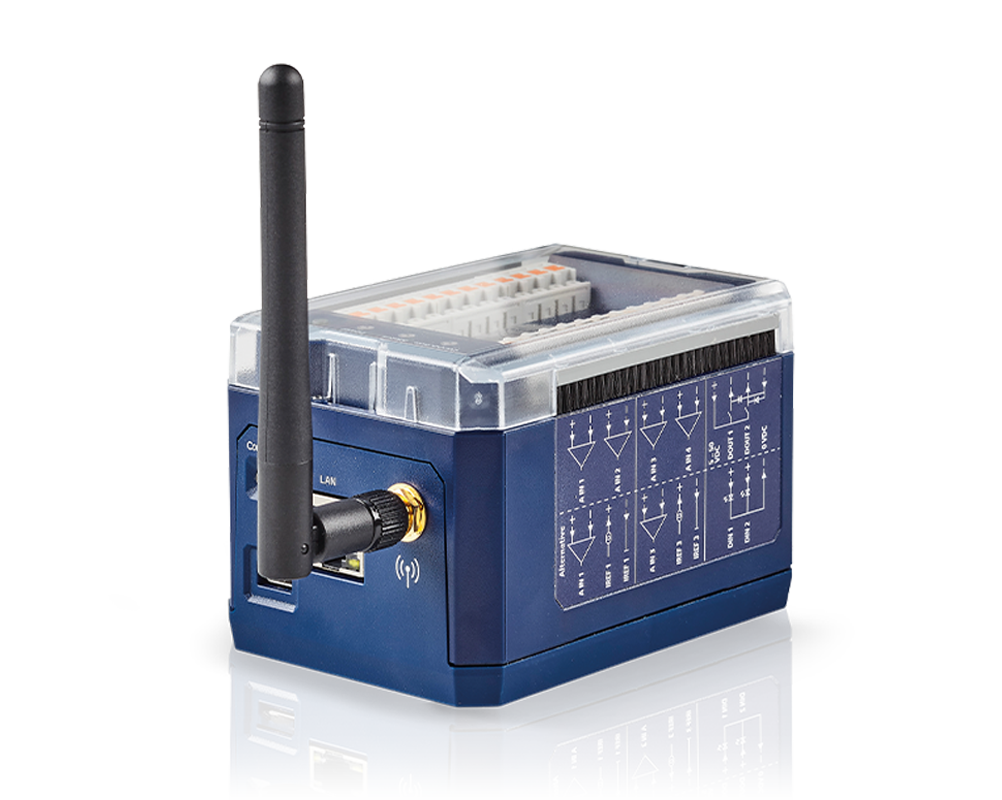
\includegraphics[height=0.3\textheight]{images/Loggito.png}
	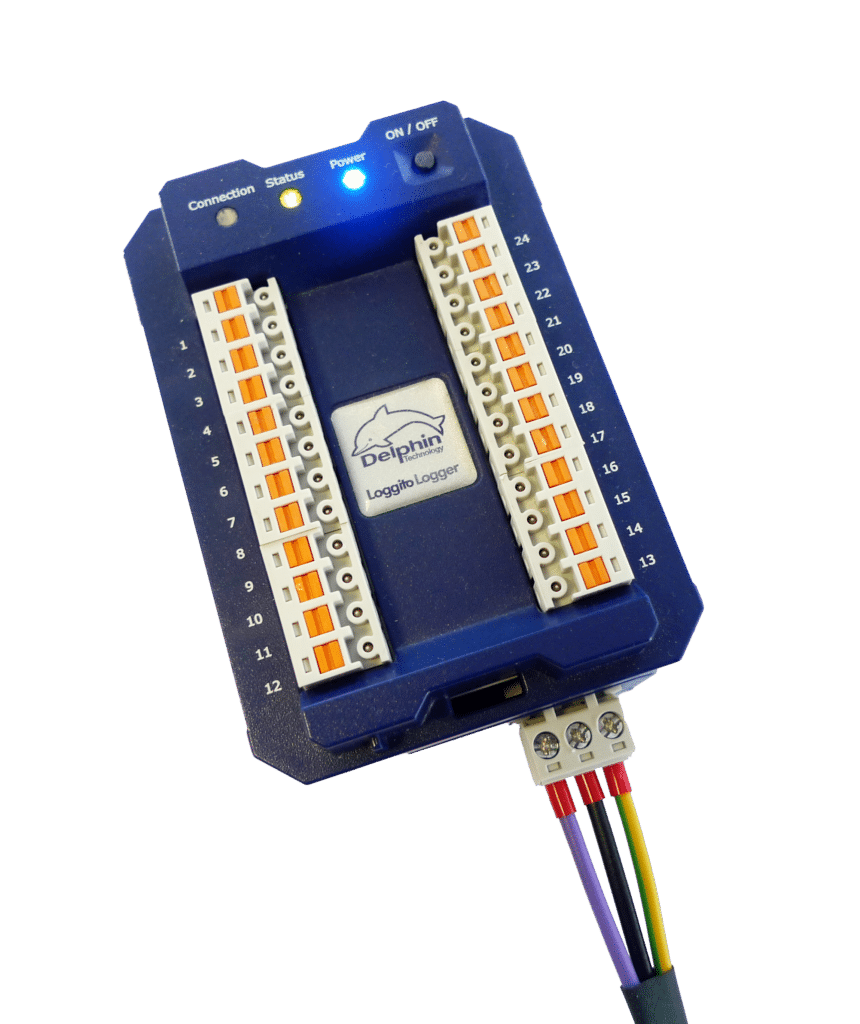
\includegraphics[height=0.3\textheight]{images/Loggito-von-oben.png}
	\caption[Bilder eines Loggito Logger von Delphin Technology.]{
		Bilder eines Loggito Logger von Delphin Technology von der Seite und von oben.
		Dabei ist der modulare Steckplatz mit 24 Eingängen sichtbar, die mit verschiedenen Modulen bestückt werden können.
		Außerdem zeigt das linke Bild eine Vielzahl von Schnittstellen, wie USB, Ethernet und WLAN.\footnotemark
	}
	\label{pic:loggito}
\end{figure}

\footnotetext{Bildquelle: \href{https://www.delphin.de/}{Delphin Technology}}

Der Datenlogger Loggito Logger von Delphin Technology~\cite{LoggitoLogger} ist wie rechts in \cref{pic:loggito} zu sehen, mit einem modularen Steckplatzsystem mit 24 Eingängen ausgestattet, sodass an diesen viele Sensoren angeschlossen werden können.
Diese einzelnen Steckplätze können mit unterschiedlichen Modulen bestückt werden, die verschiedene Schnittstellen aufweisen.
Auf der linken Seite sind weitere Schnittstellen sichtbar, unter anderem USB, Ethernet und eine Antenne für WLAN.
Somit kann der Loggito Logger mit verschiedenen Sensoren und Geräten verbunden werden und die Daten an eine zentrale Stelle senden.
In anderen Ausführungen werden auch andere Schnittstellen wie OPC UA, CAN-Bus, Profibus und RS 232/485 mit Modbus unterstützt.
Er weist einen IP67-Schutz auf, sodass er auch im Freien eingesetzt werden kann~\cite{LoggitoIP67}.
Weiterhin ist er autonom und kann auch ohne manuelle Bedienung arbeiten und erfüllt somit Teile der Anforderungen.
Gleichzeitig ist zwar eine komplexe Kombination von Messungen zu neuen Werten möglich, jedoch keine Regeldefinition und keine Steuerung.
Auch ist der Loggito Logger nicht stromsparend konzipiert, sodass ein Betrieb ohne externe Stromversorgung und somit in vielen Gärten eine Herausforderung ist.

\subsection{SCAMPI}
\emph{Sensor Configuration and Aggregation Middleware for Multi Platform Interchange} (SCAMPI) ist ein Middleware-System, das die Aggregation von Sensordaten aus heterogenen Quellen ermöglicht und in der Cloud liegt~\cite{SCAMPI}.
Dazu gehört außerdem ein regelbasiertes System zur Erzeugung virtueller Sensoren, das aus den aggregierten Daten höherwertige Informationen generieren.
Diese virtuellen Sensoren können dann wiederum als Eingabe für andere virtuelle Sensoren dienen, sodass komplexe Regelwerke erstellt werden können.
Gleichzeitig erfolgt der Zugriff auf sowohl virtuelle als auch physische Sensoren über eine einheitliche Schnittstelle, sodass die Integration von Sensoren vereinfacht wird.
Die Sensordaten können über ein Dashboard visualisiert und kombiniert werden zu Digital Twins, die den Zustand eines realen Objekts abbilden.
Als Middleware-System in der Cloud ist SCAMPI jedoch nicht nah an den Sensoren und somit müssen einfache Sensoren erst an ein Gateway angeschlossen werden, um sie in SCAMPI zu integrieren.
Weiterhin ermöglicht SCAMPI selbst keine Steuerung von Aktuatorik, sondern nur die Aggregation und Verarbeitung von Sensordaten.
Dementsprechend erfüllt SCAMPI die Anforderungen an ein universelles Sensor- und Aktuatorsystem für Smart Gardening nur teilweise.
Gleichzeitig kann SCAMPI als Grundlage für ein solches System dienen, da es die Aggregation und Verarbeitung von Sensordaten ermöglicht.

\subsection{Smart Garden Hub von GreenIQ}
Der Smart Garden Hub von GreenIQ ist ein mittlerweile eingestelltes autonomes Bewässerungssystem, das auf Wettervorhersagen und Sensoren basierend die Bewässerung bedarfsgerecht steuern kann~\cite{GreenIQ}.
Hierbei geht der Hub etwas weiter als ein reiner Sensor-Hub durch die Integration von Aktuatoren, die die Bewässerung steuern.
Als Sensoren konnten bestimmte IoT-Sensoren anderer Hersteller angeschlossen werden, die die Daten an den Smart Garden Hub senden.
Dazu gehören Wetterstationen, Regenmesser, Sonnenstandmesser und Feuchtigkeitssensoren.
Hierbei können jedoch nur IP-basierte Sensoren angeschlossen werden, was die Flexibilität einschränkt.
Dabei ist der Smart Garden Hub nur für die Bewässerung ausgelegt und kann keine anderen Aktuatoren steuern, deckt also nur einen Teil der Anwendungsfälle ab.
Weiterhin sind die Konfigurationsmöglichkeiten eingeschränkt, sodass individuelle Anpassungen schwierig sind.
Dementsprechend ist der Smart Garden Hub nur für spezifische Anwendungsfälle geeignet und kann die Anforderungen an ein universelles Sensor- und Aktuatorsystem für Smart Gardening nicht vollständig erfüllen.

\subsection{Zusammenfassung der Sensor Hubs}
Zusammengefasst ist ein Sensor-Hub ein vielseitiges Gerät, das verschiedene Sensoren und Geräte miteinander verbindet, um sowohl einfache als auch komplexe Messungen autonom durchzuführen.
Der Loggito Logger von Delphin Technology ist ein robustes und modulares Gerät, das viele Sensoren integrieren kann und mit verschiedenen Schnittstellen ausgestattet ist.
Der Universal Wireless Sensor Node von Lemos International kann eine breite Palette an Sensordaten erfassen, verarbeiten und an eine zentrale Stelle senden.
SCAMPI ist eine Middleware zur Aggregation und Verarbeitung von Sensordaten, dient also als Hub, jedoch ohne direkte Steuerungsmöglichkeiten.
Der Smart Garden Hub von GreenIQ ist auf die Bewässerung spezialisiert und integriert nur bestimmte IoT-Sensoren.
Gleichzeitig ermöglicht er eine Steuerung der Bewässerung, welche die anderen Hubs nicht bieten.
Insgesamt fehlt es den meisten Sensor-Hubs an umfassender Steuerungsintegration für ein universelles Sensor- und Aktuatorsystem für Smart Gardening.



\section{Industrial Remote Monitoring (and Control)}
Industrial Remote Monitoring bezeichnet die Fernüberwachung von industriellen Anlagen und Prozessen.
Dies kann in verschiedenen Industrien eingesetzt werden.
Dazu gehören unter anderem das verarbeitende Gewerbe, die Landwirtschaft und Transportsysteme.
Diese Systeme bestehen aus verteilter Sensorik, die die Daten an eine cloudbasierte Softwareplattform senden~\cite{IdustrialRemoteMonitoring}, wobei es sich bei der Sensorik um IoT-Sensoren handeln kann.
Hierbei werden die Daten aggregiert verarbeitet und auf Basis dieser Verarbeitung können auch Benachrichtigungen generiert werden.
Dieses Systemkonzept entspricht grob dem Sensor- und Aktuatorsystem für Smart Gardening, wobei die Aktuatorik fehlt.
Gleichzeitig bedeutet der Fokus auf die Industrie, dass solche Systeme entsprechend bepreist sind.
Auch sind sie für industrielle Skalierung ausgelegt, was häufig viel Overhead bedeutet und für einen einfachen Garten nicht verhältnismäßig ist.

\subsection{Journeo}
Das von der britischen Firma Journeo entwickelte Fernüberwachungssystem wird es hauptsächlich im öffentlichen Nah-, Bahn- und Warenverkehr und ermöglicht die Einbindung vieler IoT-Sensoren und Kameras in ein System~\cite{Journeo}.
Gleichzeitig ermöglicht dieses System keine Steuerung, sondern nur eine Fernüberwachung und ist auch nicht an den Gartenbereich angepasst.
Außerdem handelt es sich um ein kommerzielles Produkt, das nicht an Privatpersonen vertrieben wird und entsprechend teuer ist.
Somit kann es die Anforderungen an ein universelles Sensor- und Aktuatorsystem für Smart Gardening nicht vollständig erfüllen.

\subsection{Jain Unity}
Eine Erweiterung von Industrial Remote Monitoring ist Industrial Remote Monitoring and Control, bei dem auch die Steuerung von Prozessen möglich ist.
Es ist also nicht nur eine Fernüberwachung möglich, sondern auch eine Steuerung, wodurch auch Aktuatorik betrieben werden kann.

Bei Jain Unity von Jain Irrigation handelt es sich um ein automatisches Bewässerungssystem für die Landwirtschaft, welches Messungen des Bodens mit Wetterdaten und Satellitenbildern kombiniert~\cite{Jain}.
Diese Daten werden von einem KI-System für Bewässerungsentscheidungen verwendet, welche automatisch durch Öffnung entsprechender Ventile umgesetzt werden.
Dieses spezifische System erfüllt einen Teil der Anwendungsfälle, nämlich die automatische Bewässerung.
Ein Smart Gardening System besteht aber nicht nur aus einer automatischen Bewässerung, sodass dieses System nicht alle Anwendungsfälle abdeckt und daher die Anforderungen nicht erfüllen kann.
Weiterhin ist das System nicht modular erweiterbar, sondern als Gesamtsystem konzipiert, was die Anpassung an individuelle Bedürfnisse erschwert.
Außerdem ist das System auf die kommerzielle Landwirtschaft ausgelegt, was sich in der Preisgestaltung widerspiegelt und für den privaten Gartenbereich nicht geeignet ist.
Aus diesen Gründen ist das System zwar für einen spezifischen Anwendungsfall geeignet, aber nicht als ein universelles Sensor- und Aktuatorsystem für Smart Gardening.

\subsection{Zusammenfassung von Industrial Remote Monitoring (and Control)}
Zusammengefasst bezieht sich Industrial Remote Monitoring auf die Fernüberwachung industrieller Anlagen und Prozesse in verschiedenen Branchen wie dem verarbeitenden Gewerbe, der Landwirtschaft und dem Transportwesen.
Diese Systeme nutzen verteilte IoT-Sensoren, die Daten an eine meist cloudbasierte Plattform senden, wo sie verarbeitet und beispielsweise zur Generierung von Benachrichtigungen verwendet werden.
Ein Beispiel ist das Fernüberwachungssystem der Firma Journeo, das IoT-Sensoren und Kameras im Verkehrsbereich integriert, jedoch keine Steuerung ermöglicht und nicht auf den Gartenbereich zugeschnitten ist.

Eine Erweiterung dieses Konzepts ist Industrial Remote Monitoring and Control, das auch die Steuerung von Prozessen umfasst.
Ein Beispiel hierfür ist das automatische Bewässerungssystem Jain Unity, das Bodendaten, Wetterdaten und Satellitenbilder kombiniert.
Darauf basierend werden durch ein KI-System bewässerungsbezogene Entscheidungen getroffen und entsprechende Ventile automatisch gesteuert.
Obwohl dieses System für spezifische Anwendungsfälle wie die automatische Bewässerung geeignet ist, erfüllt es nicht die umfassenden Anforderungen eines modularen und universellen Sensor- und Aktuatorsystems für Smart Gardening, da es nicht modular erweiterbar ist und nur eingeschränkte Anpassungsmöglichkeiten bietet.
Da Industrial Remote Monitoring and Control aber sowohl Sensorik als auch Aktuatorik unterstützt, kann das angestrebte Sensor- und Aktuatorsystem für Smart Gardening als Remote Monitoring and Control bezeichnet werden, wobei explizit der Fokus auf den Gartenbereich und nicht auf die Industrie gelegt wird.
Gleichzeitig decken existierende Lösungen nicht alle Anwendungsfälle und Anforderungen ab.

\section{Gegenüberstellung}
In diesem Abschnitt werden die verschiedenen Systeme gegenübergestellt und anhand der funktionalen und nicht funktionalen Anforderungen bewertet.
Dafür werden die Anforderungen verwendet, die im vorherigen Kapitel aufgestellt und priorisiert wurden.

\begin{table}[!htb]
	\centering
	\caption[Konzepte und Beispiele: funktionale Anforderungen.]{
		Darstellung, welche Konzepte und Beispiele welche funktionalen Anforderungen erfüllen.
		In den Zeilen sind die verschiedenen Konzepte und Beispiele aufgeführt, in den Spalten die funktionalen Anforderungen.
		Hierbei sind die Konzepte hervorgehoben und die Beispiele sind jeweils unter den Konzepten normal aufgeführt.
		Die von einem Konzept beziehungsweise einer Realisierung erfüllten Anforderungen sind mit einem Häkchen markiert.
		Nicht erfüllte Anforderungen werden durch ein Kreuz markiert.
	}\label{tab:sdt-funkt-anforderungen}
	\begin{tabular}{llllllllll}
		\rot[\tabellenwinkel]{					} &
		\rot[\tabellenwinkel]{Messung			} &
		\rot[\tabellenwinkel]{Konfiguration		} &
		\rot[\tabellenwinkel]{Regeldefinition	} &
		\rot[\tabellenwinkel]{Dashboard			} &
		\rot[\tabellenwinkel]{Steuerung			} &
		\rot[\tabellenwinkel]{Autonomer Betrieb	} &
		\rot[\tabellenwinkel]{Benachrichtigung	} \\\hline
		\emph{IoT-Sensor}								& \OK & \NO & \NO & \NO & \NO & \OK & \NO \\
		\emph{Gateway}									& \NO & \NO & \NO & \NO & \NO & \OK & \NO \\
		\emph{Messkoffer}								& \OK & \NO & \NO & \NO & \NO & \NO & \NO \\
		Aktivitätsmesskoffer PET 2000					& \OK & \NO & \NO & \NO & \NO & \NO & \NO \\
		\emph{Sensor-Hub}								& \OK & \OK & \NO & \NO & \NO & \OK & \NO \\
		Universal Wireless Sensor Node					& \OK & \OK & \NO & \NO & \NO & \OK & \NO \\
		Loggito Logger									& \OK & \OK & \NO & \OK & \NO & \OK & \NO \\
		SCAMPI											& \OK & \OK & \OK & \OK & \NO & \OK & \NO \\
		Smart Garden Hub von GreenIQ					& \OK & \NO & \NO & \OK & \OK & \OK & \OK \\
		\emph{Industrial Remote Monitoring}				& \OK & \OK & \OK & \OK & \NO & \OK & \OK \\
		Journeo											& \OK & \OK & \NO & \OK & \NO & \OK & \OK \\
		\emph{Industrial Remote Monitoring and Control}	& \OK & \OK & \OK & \OK & \OK & \OK & \OK \\
		Jain Unity										& \OK & \NO & \NO & \OK & \OK & \OK & \OK \\
	\end{tabular}
\end{table}

Zunächst werden die funktionalen Anforderungen betrachtet, die in \cref{tab:sdt-funkt-anforderungen} dargestellt sind.
In der Tabelle sind dabei sowohl die jeweiligen Konzepte als auch Beispiele aufgeführt, wenn solche analysiert wurden.
Dabei ist zu beachten, dass die Zuordnung der Beispiele zu den Konzepten auf Basis der Beschreibung erfolgt und somit nicht immer die gleichen Anforderungen erfüllt werden.
Als Erstes fällt auf, dass kein Beispiel und nur ein Konzept, nämlich das Industrial Remote Monitoring and Control, alle funktionalen Anforderungen erfüllt.
Der IoT-Sensor und das Gateway erfüllen nur wenige Anforderungen, können aber in einem System als Grundlage für die Sensorik eingesetzt werden.
Dies steht im Gegensatz zu den Messkoffern, die nur durch manuelle Bedienung arbeiten und daher nicht in einem solchen System eingesetzt werden können.
Das Konzept des Sensor-Hubs erfüllt mehr Anforderungen, wichtige Anforderungen wie die Steuerung und Regeldefinition fehlen jedoch weiterhin.
Je nach Sensor-Hub ist eine Erweiterung potenziell möglich, sodass sie als Teil eines Smart Gardening Systems eingesetzt werden können.
Gleichzeitig erfüllen die einzelnen Beispiele für Sensor-Hubs meist weitere Anforderungen, wie SCAMPI, das auch Regeldefinitionen ermöglicht oder der Smart Garden Hub von GreenIQ welcher auch die Steuerung der Bewässerung ermöglicht.
Das Industrial Remote Monitoring erfüllt bereits die meisten funktionalen Anforderungen, jedoch fehlt die Steuerung und Journeo fehlt zusätzlich die Anforderung der Regeldefinition.
Das Industrial Remote Monitoring and Control erfüllt alle funktionalen Anforderungen, jedoch ist Jain Unity nicht modular konfigurierbar und es ermöglicht keine Regeldefinition, wodurch es nicht universell einsetzbar ist.

\begin{table}[!htb]
	\centering
	\caption[Konzepte und Beispiele: nicht funktionale Anforderungen.]{
		Darstellung, welche Konzepte und Beispiele die nicht funktionalen Anforderungen erfüllen.
		In den Zeilen sind die verschiedenen Konzepte und Beispiele aufgeführt, in den Spalten die nicht funktionalen Anforderungen.
		Die von einem Konzept / einer Realisierung erfüllten Anforderungen sind mit einem Häkchen markiert.
		In einigen Fällen ist die Erfüllung einer Anforderung nicht eindeutig, in diesen Fällen ist ein Fragezeichen markiert.
		Und in einigen Fällen ist die Anforderung nicht zutreffend, in diesen Fällen ist ein Schrägstrich markiert.
		Nicht erfüllte Anforderungen werden durch ein Kreuz markiert.
	}\label{tab:sdt-non-funkt-anforderungen}
	\begin{tabular}{lllllllllll}
		\rot[\tabellenwinkel]{						} &
		\rot[\tabellenwinkel]{Preis					} &
		\rot[\tabellenwinkel]{Elementschutz			} &
		\rot[\tabellenwinkel]{Nutzerfreundlichkeit	} &
		\rot[\tabellenwinkel]{Sicherheit			} &
		\rot[\tabellenwinkel]{Energieverbrauch		} &
		\rot[\tabellenwinkel]{Verfügbarkeit			} &
		\rot[\tabellenwinkel]{Wartbarkeit			} &
		\rot[\tabellenwinkel]{Unauffälligkeit		} \\\hline
		Aktivitätsmesskoffer							& \OK & \OK & \OK & \OK & \OK & \OK & \OK & \OK \\
		Loggito Logger									& \UN & \OK & \OK & \OK & \NO & \OK & \OK & \NO \\
		Universal Wireless Sensor Node					& \OK & \NO & \NO & \UN & \OK & \OK & \OK & \OK \\
		SCAMPI											& \OK & \NA & \OK & \OK & \NA & \OK & \OK & \NA \\
		Smart Garden Hub von GreenIQ					& \OK & \OK & \OK & \OK & \OK & \OK & \UN & \OK \\
		Journeo											& \NO & \NA & \UN & \OK & \NA & \OK & \UN & \NA \\
		Jain Unity										& \NO & \OK & \UN & \OK & \NO & \OK & \UN & \NO \\
	\end{tabular}
\end{table}

Im Folgenden werden die nicht funktionalen Anforderungen betrachtet, die in \cref{tab:sdt-non-funkt-anforderungen} dargestellt sind.
Wichtig zu beachten ist hierbei, dass hier nur die Beispiele betrachtet werden, da diese mehr als bei den funktionalen Anforderungen eine Sache der Umsetzung sind.
So definiert das Konzept des Industrial Remote Monitoring keine notwendige IP-Schutzart, diese hängt vom Umfeld des konkreten Systems ab.
Ein solches System in einer Industrieanlage ist beispielsweise anderen Bedingungen ausgesetzt als ein System in der Landwirtschaft.
Auch für die einzelnen Beispiele sind nicht alle Anforderungen direkt anwendbar.
So ist der Elementschutz für SCAMPI nicht definierbar, da es sich um eine Cloud-basierte Middleware handelt und die genutzten Sensoren nicht genauer spezifiziert sind.
Weiterhin ist die Quellenlage für einige Anforderungen bei den Beispielen nicht eindeutig, sodass diese mit einem Fragezeichen markiert sind.
Insgesamt fällt auf, dass die meisten Anforderungen für die meisten Beispiele erfüllt oder nicht anwendbar sind.

Zusammengefasst werden die funktionalen Anforderungen von keinem Beispiel vollständig erfüllt und die Beispiele, die nah herankommen, erfüllen nicht alle nicht funktionalen Anforderungen.
Gleichzeit erfüllt nur eines der Konzepte alle funktionalen Anforderungen, nämlich das Industrial Remote Monitoring and Control.
Daher ist es sinnvoll, ein eigenes System zu entwickeln, das die Anforderungen erfüllt, welches sich am Konzept des Industrial Remote Monitoring and Control orientiert und dabei den Fokus auf den Gartenbereich statt der Industrie legt.


\section{Zusammenfassung des Stands der Technik}
In diesem Kapitel wurde der Stand der Technik analysiert, der potenziell für ein universelles Sensor- und Aktuatorsystem für Smart Gardening relevant ist, und mit den Anforderungen für dieses System verglichen.
Als Konzepte wurden IoT-Sensoren, Gateways, Messkoffer, Sensor-Hubs und Industrial Remote Monitoring (and Control) betrachtet.
IoT-Sensoren und Gateways sind als Grundlage für die Sensorik eines solchen Systems geeignet, können jedoch nicht die Systemrolle übernehmen.
Messkoffer sind für Smart Gardening nicht geeignet, da sie manuell bedient werden müssen und keine Automatisierung ermöglichen.
Sensor-Hubs können als Grundlage für das System dienen, sie erfüllen jedoch die meisten Anforderungen nicht, insbesondere die Steuerung.
Gleiches gilt für die Sensor-Hubs Beispiele, welche zwar meist mehr Anforderungen erfüllen, jedoch weiterhin nicht alle.
Industrial Remote Monitoring and Control erfüllt alle funktionalen Anforderungen, dies gilt jedoch nicht für Jain Unity.
Dieses Beispiel erfüllt auch die nicht funktionalen Anforderungen nicht vollständig.
Insgesamt erfüllt kein Beispiel alle funktionalen und nicht funktionalen Anforderungen, sodass ein eigenes System entwickelt werden muss, das die Anforderungen erfüllt.
Im folgenden Kapitel wird ein Konzept für ein universelles Sensor- und Aktuatorsystem für Smart Gardening vorgestellt, das die Anforderungen erfüllt und auf den Erkenntnissen des Standes der Technik basiert.
	% !TEX root = ../thesis.tex
\chapter{Konzeption und Definition des Systems}\label{ch:konzeption}
In diesem Kapitel wird das Konzept des Systems vorgestellt sowie definiert, welcher Teil dieses Konzepts umgesetzt wird.
Dafür wird zunächst durch Nutzung eines Komponentendiagramms ein grobes Systemkonzept vorgestellt, welches die einzelnen Komponenten des Systems und deren Zusammenhänge zeigt.
Anhand von Beispielen wird das Konzept des universellen Sensor- und Aktuatorsystems für Smart Gardening erläutert und anschließend werden die einzelnen Komponenten des Systems detailliert beschrieben.

Danach wird definiert, welche Anforderungen des Systems in einem Prototyp umgesetzt werden und welche nicht.
Darauf aufbauend wird definiert, welche Komponenten und Funktionalitäten der Komponenten des Systemkonzepts im Prototyp umgesetzt werden.



\section{Modellierung des Lösungsansatzes}\label{sec:modellierung}
In diesem Abschnitt wird das Systemmodell des universellen Sensor- und Aktuatorsystems für Smart Gardening vorgestellt.
Dafür werden zunächst die übergreifenden Zusammenhänge des Systems mittels eines Diagramms erläutert und mittels eines Beispiels veranschaulicht.
Anschließend werden die einzelnen Komponenten des Systems detailliert beschrieben.

\begin{figure}[!htbp]
	\centering
	%% Creator: Inkscape 1.3.2 (091e20e, 2023-11-25, custom), www.inkscape.org
%% PDF/EPS/PS + LaTeX output extension by Johan Engelen, 2010
%% Accompanies image file 'Grobes-Konzept-Allgemein.eps' (pdf, eps, ps)
%%
%% To include the image in your LaTeX document, write
%%   \input{<filename>.pdf_tex}
%%  instead of
%%   \includegraphics{<filename>.pdf}
%% To scale the image, write
%%   \def\svgwidth{<desired width>}
%%   \input{<filename>.pdf_tex}
%%  instead of
%%   \includegraphics[width=<desired width>]{<filename>.pdf}
%%
%% Images with a different path to the parent latex file can
%% be accessed with the `import' package (which may need to be
%% installed) using
%%   \usepackage{import}
%% in the preamble, and then including the image with
%%   \import{<path to file>}{<filename>.pdf_tex}
%% Alternatively, one can specify
%%   \graphicspath{{<path to file>/}}
%% 
%% For more information, please see info/svg-inkscape on CTAN:
%%   http://tug.ctan.org/tex-archive/info/svg-inkscape
%%
\begingroup%
  \makeatletter%
  \providecommand\color[2][]{%
    \errmessage{(Inkscape) Color is used for the text in Inkscape, but the package 'color.sty' is not loaded}%
    \renewcommand\color[2][]{}%
  }%
  \providecommand\transparent[1]{%
    \errmessage{(Inkscape) Transparency is used (non-zero) for the text in Inkscape, but the package 'transparent.sty' is not loaded}%
    \renewcommand\transparent[1]{}%
  }%
  \providecommand\rotatebox[2]{#2}%
  \newcommand*\fsize{\dimexpr\f@size pt\relax}%
  \newcommand*\lineheight[1]{\fontsize{\fsize}{#1\fsize}\selectfont}%
  \ifx\svgwidth\undefined%
    \setlength{\unitlength}{328.08000183bp}%
    \ifx\svgscale\undefined%
      \relax%
    \else%
      \setlength{\unitlength}{\unitlength * \real{\svgscale}}%
    \fi%
  \else%
    \setlength{\unitlength}{\svgwidth}%
  \fi%
  \global\let\svgwidth\undefined%
  \global\let\svgscale\undefined%
  \makeatother%
  \begin{picture}(1,1.2340893)%
    \lineheight{1}%
    \setlength\tabcolsep{0pt}%
    \put(0,0){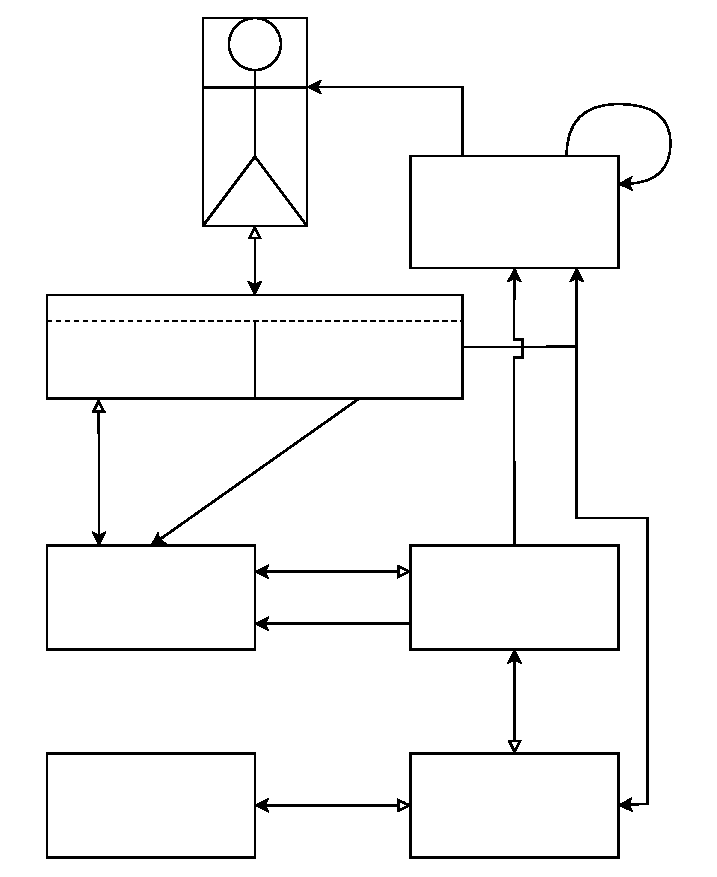
\includegraphics[width=\unitlength]{diagrams/Grobes-Konzept-Allgemein.eps}}%
    \put(0.55798345,0.5730341){\makebox(0,0)[lt]{\lineheight{1.25}\smash{\begin{tabular}[t]{l}Auslöser \&\end{tabular}}}}%
    \put(0.55579089,0.54014579){\makebox(0,0)[lt]{\lineheight{1.25}\smash{\begin{tabular}[t]{l}Herzschlag\end{tabular}}}}%
    \put(0.01638821,0.5730341){\makebox(0,0)[lt]{\lineheight{1.25}\smash{\begin{tabular}[t]{l}Daten-\end{tabular}}}}%
    \put(0.01128367,0.54014579){\makebox(0,0)[lt]{\lineheight{1.25}\smash{\begin{tabular}[t]{l}anfrage\end{tabular}}}}%
    \put(0.13040104,0.5730341){\makebox(0,0)[lt]{\lineheight{1.25}\smash{\begin{tabular}[t]{l}Daten-\end{tabular}}}}%
    \put(0.12676962,0.54014579){\makebox(0,0)[lt]{\lineheight{1.25}\smash{\begin{tabular}[t]{l}antwort\end{tabular}}}}%
    \put(0.376344,0.46340638){\makebox(0,0)[lt]{\lineheight{1.25}\smash{\begin{tabular}[t]{l}Konfiguration\end{tabular}}}}%
    \put(0.40046212,0.43051805){\makebox(0,0)[lt]{\lineheight{1.25}\smash{\begin{tabular}[t]{l}Anfragen\end{tabular}}}}%
    \put(0.74322003,0.24195836){\makebox(0,0)[lt]{\lineheight{1.25}\smash{\begin{tabular}[t]{l}Daten-\end{tabular}}}}%
    \put(0.73958863,0.20907006){\makebox(0,0)[lt]{\lineheight{1.25}\smash{\begin{tabular}[t]{l}antwort\end{tabular}}}}%
    \put(0.7962182,1.11898018){\makebox(0,0)[lt]{\lineheight{1.25}\smash{\begin{tabular}[t]{l}Selbstauslöser\end{tabular}}}}%
    \put(0.83458792,0.75940123){\makebox(0,0)[lt]{\lineheight{1.25}\smash{\begin{tabular}[t]{l}Konfigu-\end{tabular}}}}%
    \put(0.84993578,0.72651293){\makebox(0,0)[lt]{\lineheight{1.25}\smash{\begin{tabular}[t]{l}rieren\end{tabular}}}}%
    \put(0.18192607,0.86683642){\makebox(0,0)[lt]{\lineheight{1.25}\smash{\begin{tabular}[t]{l}Interaktion\end{tabular}}}}%
    \put(0.41981824,0.12136786){\makebox(0,0)[lt]{\lineheight{1.25}\smash{\begin{tabular}[t]{l}Daten-\end{tabular}}}}%
    \put(0.41471372,0.08847956){\makebox(0,0)[lt]{\lineheight{1.25}\smash{\begin{tabular}[t]{l}anfrage\end{tabular}}}}%
    \put(0.42091452,0.05559123){\makebox(0,0)[lt]{\lineheight{1.25}\smash{\begin{tabular}[t]{l}Daten-\end{tabular}}}}%
    \put(0.4172831,0.02270292){\makebox(0,0)[lt]{\lineheight{1.25}\smash{\begin{tabular}[t]{l}antwort\end{tabular}}}}%
    \put(0.4947762,1.14529084){\makebox(0,0)[lt]{\lineheight{1.25}\smash{\begin{tabular}[t]{l}Nachricht\end{tabular}}}}%
    \put(0.14102123,0.08847956){\makebox(0,0)[lt]{\lineheight{1.25}\smash{\begin{tabular}[t]{l}Externe\end{tabular}}}}%
    \put(0.10881808,0.05559123){\makebox(0,0)[lt]{\lineheight{1.25}\smash{\begin{tabular}[t]{l}Datenquellen\end{tabular}}}}%
    \put(0.12382338,0.3757042){\makebox(0,0)[lt]{\lineheight{1.25}\smash{\begin{tabular}[t]{l}Datenbank\end{tabular}}}}%
    \put(0.63653856,0.39105207){\makebox(0,0)[lt]{\lineheight{1.25}\smash{\begin{tabular}[t]{l}Sensor- und\end{tabular}}}}%
    \put(0.62653502,0.35816376){\makebox(0,0)[lt]{\lineheight{1.25}\smash{\begin{tabular}[t]{l}Aktuatorkoffer\end{tabular}}}}%
    \put(0.58751442,0.94138326){\makebox(0,0)[lt]{\lineheight{1.25}\smash{\begin{tabular}[t]{l}Benachrichtigungen\end{tabular}}}}%
    \put(0.376344,0.38885951){\makebox(0,0)[lt]{\lineheight{1.25}\smash{\begin{tabular}[t]{l}Konfiguration\end{tabular}}}}%
    \put(0.41070544,0.35597121){\makebox(0,0)[lt]{\lineheight{1.25}\smash{\begin{tabular}[t]{l}senden\end{tabular}}}}%
    \put(0.65812152,0.10382744){\makebox(0,0)[lt]{\lineheight{1.25}\smash{\begin{tabular}[t]{l}Server für\end{tabular}}}}%
    \put(0.67199629,0.07313167){\makebox(0,0)[lt]{\lineheight{1.25}\smash{\begin{tabular}[t]{l}externe\end{tabular}}}}%
    \put(0.63835429,0.04024334){\makebox(0,0)[lt]{\lineheight{1.25}\smash{\begin{tabular}[t]{l}Datenquellen\end{tabular}}}}%
    \put(0.20663815,0.47409399){\rotatebox{35.00000068}{\makebox(0,0)[lt]{\lineheight{1.25}\smash{\begin{tabular}[t]{l}Konfiguration speichern\end{tabular}}}}}%
    \put(0.62262955,0.24195836){\makebox(0,0)[lt]{\lineheight{1.25}\smash{\begin{tabular}[t]{l}Daten-\end{tabular}}}}%
    \put(0.61752501,0.20907006){\makebox(0,0)[lt]{\lineheight{1.25}\smash{\begin{tabular}[t]{l}anfrage\end{tabular}}}}%
    \put(0.42533389,0.32089033){\makebox(0,0)[lt]{\lineheight{1.25}\smash{\begin{tabular}[t]{l}Daten\end{tabular}}}}%
    \put(0.4172831,0.288002){\makebox(0,0)[lt]{\lineheight{1.25}\smash{\begin{tabular}[t]{l}senden\end{tabular}}}}%
    \put(0.12091139,0.72432038){\makebox(0,0)[lt]{\lineheight{1.25}\smash{\begin{tabular}[t]{l}Dashboard\end{tabular}}}}%
    \put(0.40046212,0.74624592){\makebox(0,0)[lt]{\lineheight{1.25}\smash{\begin{tabular}[t]{l}Konfigurations-\end{tabular}}}}%
    \put(0.43263099,0.71335759){\makebox(0,0)[lt]{\lineheight{1.25}\smash{\begin{tabular}[t]{l}werkzeug\end{tabular}}}}%
    \put(0.229066,0.79667466){\makebox(0,0)[lt]{\lineheight{1.25}\smash{\begin{tabular}[t]{l}Nutzerschnittstelle\end{tabular}}}}%
  \end{picture}%
\endgroup%

	\caption[Darstellung des übergreifenden Systemkonzepts.]{
		Darstellung des übergreifenden Systemkonzepts des universellen Sensor- und Aktuatorsystems für Smart Gardening mit Überblick über die Komponenten und Schnittstellen.
		Dabei sind die Komponenten des Systems in Boxen dargestellt und Pfeile stellen die Datenflüsse zwischen den Komponenten dar.
		Hat ein Pfeil eine nicht ausgefüllte Pfeilspitze, stellt diese die Antwort auf eine Anfrage dar.
		Die zu Anfragen dazugehörige Beschriftung befindet sich über oder links eines Pfeils, die zu Antworten unter oder rechts eines Pfeils.
		Die Komponente Sensor- und Aktuatorkoffer ist selbst in weitere Komponenten unterteilt, die in \cref{pic:koffer-konzept} dargestellt sind.
		}
	\label{pic:systemkonzept}
\end{figure}

Das Systemkonzept besteht aus mehreren Komponenten, die miteinander interagieren, um die verschiedenen Anforderungen und Anwendungsfälle abdecken zu können.
Dieses ist in \cref{pic:systemkonzept} dargestellt und wird anhand der Abbildung im Folgenden erläutert.
Zu diesen Komponenten gehören der Sensor- und Aktuatorkoffer, die Datenbank, die Nutzerschnittstelle, die Benachrichtigungen und der Server für externe Datenquellen.
An oberster Stelle steht dabei der Nutzer, welcher über die Nutzerschnittstelle mit dem System interagiert, wobei diese weiter in ein Dashboard und ein Konfigurationswerkzeug unterteilt ist.
Das Dashboard dient dabei der Anzeige von Informationen und der Steuerung des Systems, während das Konfigurationswerkzeug der Konfiguration des Systems dient.
Hierbei greift das Dashboard auf die Datenbank zu, um die benötigten Informationen anzuzeigen.
Das Konfigurationswerkzeug kann den Sensor- und Aktuatorkoffer, die Benachrichtigungen und den Server für externe Datenquellen konfigurieren.
Der Sensor- und Aktuatorkoffer ist dabei die zentrale Komponente des Systems, welche die Sensorik und Aktuatorik steuert, Regeln ausführt und Daten an die Datenbank sendet.
Gleichzeitig kann der Sensor- und Aktuatorkoffer auch Daten von externen Datenquellen über den Server für externe Datenquellen anfragen, um diese in die Regelverarbeitung einzubeziehen.
Außerdem kann er Benachrichtigungen an den Nutzer auslösen, wenn bestimmte Bedingungen erfüllt sind.
Der Server für externe Datenquellen dient dabei als Schnittstelle zu externen Datenquellen wie Wetterdiensten, um hier eine homogene Schnittstelle für den Sensor- und Aktuatorkoffer zu schaffen.

Anhand eines Beispiels kann das wie folgt aussehen.  % Den Satz einmal verbessern
Ein Nutzer baut das System auf, verbindet verschiedene Sensoren und Aktuatoren mit dem Sensor- und Aktuatorkoffer und konfiguriert das System über das Konfigurationswerkzeug.
Dabei legt er eine Regel zur automatischen Bewässerung an, welche die Bodenfeuchtigkeit und Wetterdaten überwacht und beim Unterschreiten eines Schwellenwerts automatisch die Bewässerung startet und den Nutzer benachrichtigt.
Der Sensor- und Aktuatorkoffer führt diese Regel periodisch aus und sendet in regelmäßigen Abständen einen Herzschlag, um den Betrieb zu bestätigen.
Zur Ausführung dieser Regel greift der Sensor- und Aktuatorkoffer auf den Server für externe Datenquellen zu, um die aktuellen Wetterdaten anzufragen.
Diese werden von dem Server aus einer externen Datenquelle bezogen und an den Sensor- und Aktuatorkoffer weitergeleitet.
Die generierten Messdaten werden an die Datenbank gesendet und durch das Dashboard als digitaler Zwilling seines Gartens für den Nutzer visualisiert.
Wird nun eine Bewässerung durch den Sensor- und Aktuatorkoffer ausgelöst, schickt dieser eine Benachrichtigung an die Benachrichtigungskomponente, welche den Nutzer über die von ihm konfigurierten Quellen informiert.

In den folgenden Abschnitten werden die einzelnen Komponenten näher erläutert und die Schnittstellen zwischen den Komponenten definiert, beginnend mit dem Sensor- und Aktuatorkoffer, der als zentrale Komponente des Systems fungiert.
Darauf folgen die Datenbank, die Nutzerschnittstelle, die Benachrichtigungen und der Server für externe Datenquellen.
Anschließend wird das Systemkonzept zusammengefasst.


\subsection{Erklärung der Systemkomponente Sensor- und Aktuatorkoffer}
In diesem Abschnitt wird die Systemkomponente Sensor- und Aktuatorkoffer genauer erläutert, welche als zentrale Komponente des Systems fungiert.
Dabei wird der Sensor- und Aktuatorkoffer selbst in weitere Komponenten unterteilt, welche die Funktionalität des Sensor- und Aktuatorkoffers bereitstellen.
Diese werden anhand eines Diagramms und eines Beispiels genauer erläutert.

\begin{figure}[!htbp]
	\centering
	%% Creator: Inkscape 1.3.2 (091e20e, 2023-11-25, custom), www.inkscape.org
%% PDF/EPS/PS + LaTeX output extension by Johan Engelen, 2010
%% Accompanies image file 'KofferKonzept.eps' (pdf, eps, ps)
%%
%% To include the image in your LaTeX document, write
%%   \input{<filename>.pdf_tex}
%%  instead of
%%   \includegraphics{<filename>.pdf}
%% To scale the image, write
%%   \def\svgwidth{<desired width>}
%%   \input{<filename>.pdf_tex}
%%  instead of
%%   \includegraphics[width=<desired width>]{<filename>.pdf}
%%
%% Images with a different path to the parent latex file can
%% be accessed with the `import' package (which may need to be
%% installed) using
%%   \usepackage{import}
%% in the preamble, and then including the image with
%%   \import{<path to file>}{<filename>.pdf_tex}
%% Alternatively, one can specify
%%   \graphicspath{{<path to file>/}}
%% 
%% For more information, please see info/svg-inkscape on CTAN:
%%   http://tug.ctan.org/tex-archive/info/svg-inkscape
%%
\begingroup%
  \makeatletter%
  \providecommand\color[2][]{%
    \errmessage{(Inkscape) Color is used for the text in Inkscape, but the package 'color.sty' is not loaded}%
    \renewcommand\color[2][]{}%
  }%
  \providecommand\transparent[1]{%
    \errmessage{(Inkscape) Transparency is used (non-zero) for the text in Inkscape, but the package 'transparent.sty' is not loaded}%
    \renewcommand\transparent[1]{}%
  }%
  \providecommand\rotatebox[2]{#2}%
  \newcommand*\fsize{\dimexpr\f@size pt\relax}%
  \newcommand*\lineheight[1]{\fontsize{\fsize}{#1\fsize}\selectfont}%
  \ifx\svgwidth\undefined%
    \setlength{\unitlength}{369.12000275bp}%
    \ifx\svgscale\undefined%
      \relax%
    \else%
      \setlength{\unitlength}{\unitlength * \real{\svgscale}}%
    \fi%
  \else%
    \setlength{\unitlength}{\svgwidth}%
  \fi%
  \global\let\svgwidth\undefined%
  \global\let\svgscale\undefined%
  \makeatother%
  \begin{picture}(1,1.13784134)%
    \lineheight{1}%
    \setlength\tabcolsep{0pt}%
    \put(0,0){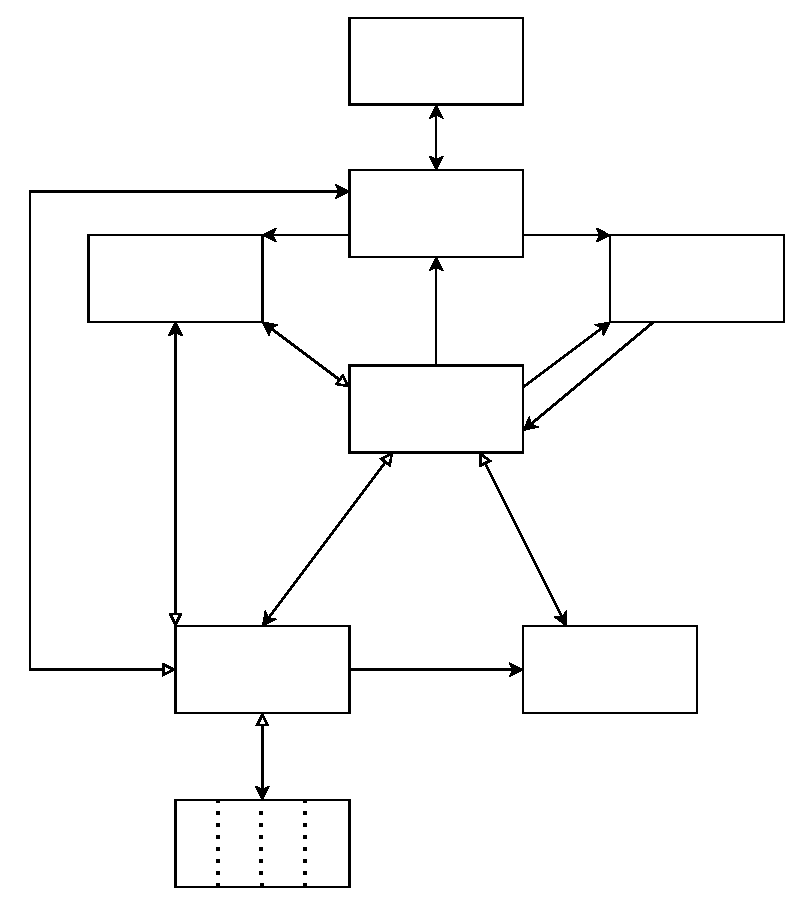
\includegraphics[width=\unitlength]{diagrams/KofferKonzept.eps}}%
    \put(0.36229892,0.75268833){\rotatebox{-37.00000005}{\makebox(0,0)[lt]{\lineheight{1.25}\smash{\begin{tabular}[t]{l}Regel\end{tabular}}}}}%
    \put(0.33445225,0.73951302){\rotatebox{-37.00000005}{\makebox(0,0)[lt]{\lineheight{1.25}\smash{\begin{tabular}[t]{l}anfragen\end{tabular}}}}}%
    \put(0.29118764,0.71969367){\rotatebox{-37.00000005}{\makebox(0,0)[lt]{\lineheight{1.25}\smash{\begin{tabular}[t]{l}Regel senden\end{tabular}}}}}%
    \put(0.66688184,0.62147216){\rotatebox{39.00000116}{\makebox(0,0)[lt]{\lineheight{1.25}\smash{\begin{tabular}[t]{l}Regel auslösen\end{tabular}}}}}%
    \put(0.67293725,0.71663924){\rotatebox{35.99999868}{\makebox(0,0)[lt]{\lineheight{1.25}\smash{\begin{tabular}[t]{l}Job\end{tabular}}}}}%
    \put(0.67209931,0.68230949){\rotatebox{35.99999868}{\makebox(0,0)[lt]{\lineheight{1.25}\smash{\begin{tabular}[t]{l}anlegen\end{tabular}}}}}%
    \put(0.46048854,0.76662729){\makebox(0,0)[lt]{\lineheight{1.25}\smash{\begin{tabular}[t]{l}Daten\end{tabular}}}}%
    \put(0.45394235,0.73934647){\makebox(0,0)[lt]{\lineheight{1.25}\smash{\begin{tabular}[t]{l}senden\end{tabular}}}}%
    \put(0.63499902,0.5214145){\rotatebox{-62.99999795}{\makebox(0,0)[lt]{\lineheight{1.25}\smash{\begin{tabular}[t]{l}Datenantwort\end{tabular}}}}}%
    \put(0.59405085,0.52215864){\rotatebox{-62.99999795}{\makebox(0,0)[lt]{\lineheight{1.25}\smash{\begin{tabular}[t]{l}Datenanfrage\end{tabular}}}}}%
    \put(0.29373901,0.38109393){\rotatebox{52.99999995}{\makebox(0,0)[lt]{\lineheight{1.25}\smash{\begin{tabular}[t]{l}Sensorik anfragen\end{tabular}}}}}%
    \put(0.31158684,0.3594479){\rotatebox{52.99999995}{\makebox(0,0)[lt]{\lineheight{1.25}\smash{\begin{tabular}[t]{l}Aktuatorik auslösen\end{tabular}}}}}%
    \put(0.34596253,0.34802111){\rotatebox{52.99999995}{\makebox(0,0)[lt]{\lineheight{1.25}\smash{\begin{tabular}[t]{l}Ergebnismeldung\end{tabular}}}}}%
    \put(0.44225059,0.29505876){\makebox(0,0)[lt]{\lineheight{1.25}\smash{\begin{tabular}[t]{l}Daten speichern\end{tabular}}}}%
    \put(0.16700054,0.3587181){\rotatebox{90}{\makebox(0,0)[lt]{\lineheight{1.25}\smash{\begin{tabular}[t]{l}Sensor- / Aktuatordefinition\end{tabular}}}}}%
    \put(0.19428137,0.44506678){\rotatebox{90}{\makebox(0,0)[lt]{\lineheight{1.25}\smash{\begin{tabular}[t]{l}anfragen\end{tabular}}}}}%
    \put(0.2390998,0.35871808){\rotatebox{90}{\makebox(0,0)[lt]{\lineheight{1.25}\smash{\begin{tabular}[t]{l}Sensor- / Aktuatordefinition\end{tabular}}}}}%
    \put(0.26638063,0.45106489){\rotatebox{90}{\makebox(0,0)[lt]{\lineheight{1.25}\smash{\begin{tabular}[t]{l}Antwort\end{tabular}}}}}%
    \put(0.34119583,0.97318209){\makebox(0,0)[lt]{\lineheight{1.25}\smash{\begin{tabular}[t]{l}Kommunikation\end{tabular}}}}%
    \put(0.25582146,0.87380195){\makebox(0,0)[lt]{\lineheight{1.25}\smash{\begin{tabular}[t]{l}Konfigurieren\end{tabular}}}}%
    \put(0.66454665,0.86990468){\makebox(0,0)[lt]{\lineheight{1.25}\smash{\begin{tabular}[t]{l}Job anlegen\end{tabular}}}}%
    \put(0.15552789,0.17229505){\makebox(0,0)[lt]{\lineheight{1.25}\smash{\begin{tabular}[t]{l}Ansteuerung\end{tabular}}}}%
    \put(0.32405396,0.17034641){\makebox(0,0)[lt]{\lineheight{1.25}\smash{\begin{tabular}[t]{l}Ergebnis\end{tabular}}}}%
    \put(0.21876703,0.05147997){\makebox(0,0)[lt]{\lineheight{1.25}\smash{\begin{tabular}[t]{l}S1\end{tabular}}}}%
    \put(0.39149484,0.05147997){\makebox(0,0)[lt]{\lineheight{1.25}\smash{\begin{tabular}[t]{l}...\end{tabular}}}}%
    \put(0.03666145,0.29895601){\makebox(0,0)[lt]{\lineheight{1.25}\smash{\begin{tabular}[t]{l}Ansteuerung\end{tabular}}}}%
    \put(0.07268066,0.2658293){\makebox(0,0)[lt]{\lineheight{1.25}\smash{\begin{tabular}[t]{l}Ergebnis\end{tabular}}}}%
    \put(0.32983897,0.05147997){\makebox(0,0)[lt]{\lineheight{1.25}\smash{\begin{tabular}[t]{l}A1\end{tabular}}}}%
    \put(0.70147929,0.28141834){\makebox(0,0)[lt]{\lineheight{1.25}\smash{\begin{tabular}[t]{l}Datenbank\end{tabular}}}}%
    \put(0.26185003,0.30869916){\makebox(0,0)[lt]{\lineheight{1.25}\smash{\begin{tabular}[t]{l}Sensor \&\end{tabular}}}}%
    \put(0.26602133,0.28141834){\makebox(0,0)[lt]{\lineheight{1.25}\smash{\begin{tabular}[t]{l}Aktuator\end{tabular}}}}%
    \put(0.24814873,0.2521889){\makebox(0,0)[lt]{\lineheight{1.25}\smash{\begin{tabular}[t]{l}Schnittstelle\end{tabular}}}}%
    \put(0.49032692,1.08620265){\makebox(0,0)[lt]{\lineheight{1.25}\smash{\begin{tabular}[t]{l}Restliches\end{tabular}}}}%
    \put(0.50402824,1.05697319){\makebox(0,0)[lt]{\lineheight{1.25}\smash{\begin{tabular}[t]{l}System\end{tabular}}}}%
    \put(0.81644849,0.78806221){\makebox(0,0)[lt]{\lineheight{1.25}\smash{\begin{tabular}[t]{l}Scheduler\end{tabular}}}}%
    \put(0.12337549,0.79001084){\makebox(0,0)[lt]{\lineheight{1.25}\smash{\begin{tabular}[t]{l}Definitionen\end{tabular}}}}%
    \put(0.45397279,0.62048002){\makebox(0,0)[lt]{\lineheight{1.25}\smash{\begin{tabular}[t]{l}Regelausführer\end{tabular}}}}%
    \put(0.27235437,0.05147997){\makebox(0,0)[lt]{\lineheight{1.25}\smash{\begin{tabular}[t]{l}S2\end{tabular}}}}%
    \put(0.46310699,0.87575058){\makebox(0,0)[lt]{\lineheight{1.25}\smash{\begin{tabular}[t]{l}Schnittstelle\end{tabular}}}}%
  \end{picture}%
\endgroup%

	\caption[Darstellung der Systemkomponente Sensor- und Aktuatorkoffer.]{
		Darstellung der Systemkomponente Sensor- und Aktuatorkoffer mit Überblick über die Komponenten und Schnittstellen.
		Dabei sind die Komponenten des Systems in Boxen dargestellt und Pfeile stellen die Datenflüsse zwischen den Komponenten dar.
		Hat ein Pfeil eine nicht ausgefüllte Pfeilspitze, stellt diese die Antwort auf eine Anfrage dar.
		Die zu Anfragen dazugehörige Beschriftung befindet sich über oder links eines Pfeils, die zu Antworten unter oder rechts eines Pfeils.
		}
	\label{pic:koffer-konzept}
\end{figure}

Der Sensor- und Aktuatorkoffer besteht aus unterschiedlichen Komponenten und Schnittstellen, welche die Funktionalität des Sensor- und Aktuatorkoffers bereitstellen.
Diese sind in \cref{pic:koffer-konzept} dargestellt und werden im Folgenden anhand der Abbildung erläutert.
Die zentrale Komponente des Sensor- und Aktuatorkoffers ist der Regelausführer, welcher durch die Ausführung von Regeln die Steuerung des Sensor- und Aktuatorkoffers übernimmt.
Die Ausführung einer Regel wird dabei durch den Scheduler gesteuert, welcher die zeitliche Planung der Regelausführung übernimmt.
Außerdem greift der Regelausführer auf die Sensor- und Aktuatorschnittstelle zu, um die Sensorik und Aktuatorik anzusteuern und Messdaten zu erfassen.
In den Definitionen werden die unterschiedlichen Regeln und die unterschiedlichen Sensoren und Aktuatoren definiert, welche im Sensor- und Aktuatorkoffer verwendet werden.
Die Komponenten fragen diese Definitionen an, wenn sie benötigt werden, um ihre Funktion auszuüben.
Stehen die Messdaten zur Verfügung, werden diese in der Datenbank gespeichert, um sie für die weitere Verarbeitung bereitzustellen.

Zur Veranschaulichung mittels eines Beispiels wird das vorherige Beispiel mit der Bewässerungsregel für die Sensor- und Aktuatorkofferkomponente fortgeführt.
Der Sensor- und Aktuatorkoffer erfragt die Konfiguration über die Schnittstelle und legt die Regel und die Sensor- und Aktuatordefinitionen in den Definitionen ab.
Gleichzeitig wird im Scheduler die Regel als Job angelegt, der periodisch ausgeführt wird.
Löst der Scheduler diese Regel nun aus, greift der Regelausführer auf die Definitionen zu und lädt die Regeldefinition.
In diesem Fall beinhaltet die Regeldefinition die Bedingung, dass die Bodenfeuchtigkeit unter einen Schwellenwert fällt und die Wetterdaten keinen Regen vorhersagen, um eine Bewässerung auszulösen und eine Benachrichtigung zu verschicken.
Der Regelausführer fragt nun die Sensor- und Aktuatorschnittstelle ab, um die aktuellen Messdaten zu erhalten.
Diese holt sich die Definition für den Bodenfeuchtigkeitssensor und den Wetterdienst von den Definitionen und fragt die Sensoren ab.
Das Ergebnis wird in der Datenbank gespeichert und der Regelausführer kann die Bedingung nun prüfen.
Für dieses Beispiel wird angenommen, dass die Bedingung erfüllt ist und die Bewässerung ausgelöst wird.
Der Regelausführer weist nun die Sensor- und Aktuatorschnittstelle an, die Bewässerung zu starten, wo der Vorgang analog zum Vorgang für die Sensorik läuft.
Sobald dies beendet ist, löst der Regelausführer über die Schnittstelle zum restlichen System eine Benachrichtigung aus.

Im Folgenden werden die einzelnen Komponenten des Sensor- und Aktuatorkoffers detailliert erläutert, beginnend mit dem Scheduler.
Darauf folgen der Regelausführer, die Schnittstelle, die Definitionen, die Datenbank und die Sensor- und Aktuatorschnittstelle.

\subsubsection{Erklärung der Kofferkomponente Scheduler}
Der Scheduler ist die Komponente des Sensor- und Aktuatorkoffers, die den Takt angibt und steuert, wann welche Regeln ausgeführt werden.
Eine solche einmalige oder periodische Anlegung von Regeln wird als Job bezeichnet.
Dafür bietet der Scheduler eine Schnittstelle an, über die Regeln angelegt, geändert und gelöscht werden können.
Die Komponente kennt dabei nur die ID der Regel und den Zeitpunkt, zu dem die Regel ausgeführt werden soll, wobei dieser auch periodisch sein kann.
Dabei ist es wichtig, dass der Scheduler die Zeitzone des Systems berücksichtigt, um die Regeln korrekt auszuführen.
Soll eine Regel ausgeführt werden, ruft der Scheduler den Regelausführer mit der ID der Regel auf, um die Regel auszuführen.
Außerdem muss der Scheduler so funktionieren, dass er auch bei einem Schlafmodus des Systems zum Sparen von Energie weiterhin Regeln ausführen kann.

\subsubsection{Erklärung der Kofferkomponente Regelausführer}
Der Regelausführer stellt die zentrale Komponente des Sensor- und Aktuatorkoffers dar, welche durch die Ausführung von Regeln die Steuerung des Sensor- und Aktuatorkoffers übernimmt.
Die Regeln müssen ein bestimmtes Format einhalten, welches in \cref{sec:definitionsformat} definiert ist.
Der Regelausführer ist zwar mit allen weiteren Komponenten verbunden, weist jedoch nur eine Schnittstelle auf.
Über diese kann durch Übergabe der ID der Regel die Regelausführung gestartet werden.
Diese beginnt mit dem Laden der Regeldefinition aus den Definitionen durch Übergabe der ID der Regel.
Anschließend wird die Regel ausgeführt, welche mehrere Schritte umfassen kann.
Zunächst kann eine Messung mit einem Sensor durchgeführt werden, wofür die Sensor- und Aktuatorschnittstelle mit der ID des Sensors aufgerufen wird.
Der Regelausführer wartet darauf, dass die Messung abgeschlossen ist und fährt dann mit der weiteren Verarbeitung der Regel fort.
Eine Regel kann auch eine Aktion mit einem Aktuator auslösen, wofür die Sensor- und Aktuatorschnittstelle mit der ID des Aktuators aufgerufen wird.
Auch hier wartet der Regelausführer darauf, dass die Aktion abgeschlossen ist und fährt dann mit der weiteren Verarbeitung der Regel fort.
Sollte die Regel eine Benachrichtigung auslösen, wird die Benachrichtigungskomponente des Gesamtsystems über die Schnittstelle mit der ID der Benachrichtigung aufgerufen.
Weiterhin kann die Regel selbst einen Job im Scheduler anlegen.
Die letzte Option ist das Abrufen von Daten aus der lokalen Datenbank, die zum einen für die Verarbeitung der Regel verwendet und zum anderen an die Datenbank des Gesamtsystems gesendet werden können.

\subsubsection{Erklärung der Kofferkomponente Sensor- und Aktuatorkofferschnittstelle}
Die Schnittstelle des Sensor- und Aktuatorkoffers stellt die Verbindung zu den anderen Komponenten des Gesamtsystems her.
Dabei bietet sie dem Sensor- und Aktuatorkoffer unterschiedliche Methoden an, um die verschiedenen Funktionen zu realisieren.
Welche Kommunikationsarten genau unterstützt werden, ist ein Implementierungsdetail.
Gleichzeitig ist die Schnittstelle auch für den Herzschlag des Sensor- und Aktuatorkoffers zuständig, welcher periodisch an das Gesamtsystem gesendet wird, um den Betrieb zu bestätigen.
Um eine Nachricht zu senden, muss der Schnittstelle die Komponente und die Nachricht übergeben werden.
Die Antwort wird der Komponente zurückgegeben, welche die Nachricht gesendet hat.

\subsubsection{Erklärung der Kofferkomponente Definitionen}
Die Definitionen des Sensor- und Aktuatorkoffers enthalten die Definitionen für die Regeln, Sensoren und Aktuatoren, welche im Sensor- und Aktuatorkoffer verwendet werden.
Sie werden in einem Schlüssel-Werte-Format abgelegt, wobei der Schlüssel die ID der Definition ist und der Wert die Definition selbst.
Das genaue Format für die Regeln und die Sensor- und Aktuatordefinitionen ist in \cref{sec:definitionsformat} definiert.
Die Definitionen werden über die Schnittstelle angefragt, wobei die ID der Definition übergeben wird.
Außerdem können die Definitionen auch über die Schnittstelle konfiguriert, also angelegt, geändert und gelöscht werden.

\subsubsection{Erklärung der Kofferkomponente Datenbank}
Die Datenbank des Sensor- und Aktuatorkoffers dient dazu, die Messdaten der Sensoren und Ergebnisse der Aktuatoren temporär zu speichern.
Diese Daten werden zum einen für die Verarbeitung der Regeln benötigt und zum anderen an die Datenbank des Gesamtsystems gesendet, um sie dort dauerhaft zu speichern.
Die lokale Datenbank kann die Daten aufgrund der knappen lokalen Ressourcen nur temporär speichern, wobei die Speicherdauer von der Implementierung und den genutzten Regeln abhängt.
Wird der Speicherplatz knapp, werden die ältesten Daten gelöscht, um Platz für neue Daten zu schaffen.
Zwei Schnittstellen werden für die Datenbank benötigt, eine zum Speichern der Daten und eine zum Abrufen der Daten.
Für das Abfragen der Daten kann zum einen die Datenquelle und zum anderen der Zeitraum angegeben werden, für den die Daten abgefragt werden sollen.

\subsubsection{Erklärung der Kofferkomponente Sensor- und Aktuatorschnittstelle}
Die Sensor- und Aktuatorschnittstelle des Sensor- und Aktuatorkoffers dient dazu, die Sensorik und Aktuatorik anzusteuern und Messdaten zu erfassen.
Dafür kann der Nutzer bei der Konfiguration des Systems unterschiedliche Sensoren und Aktuatoren an den Sensor- und Aktuatorkoffer anschließen und diese über das Konfigurationswerkzeug konfigurieren.
Auch externe Datenquellen können virtuell als Sensoren und Aktuatoren an den Sensor- und Aktuatorkoffer angeschlossen werden, sodass deren Nutzung identisch zu lokalen Sensoren und Aktuatoren ist.
Die Sensor- und Aktuatorschnittstelle bietet dafür eine Schnittstelle an, über die durch Übergabe der ID des Sensors oder Aktuators die Messung oder Aktion gestartet werden kann.
Anschließend fragt sie die Definition des Sensors oder Aktuators aus den Definitionen ab und führt die Messung oder Aktion durch Ansteuerung des Sensors oder Aktuators aus, woraufhin die Messdaten zurückgegeben werden.


\subsection{Erklärung der Systemkomponente Datenbank}
Die Datenbank des Gesamtsystems dient dazu, die Messdaten der Sensoren, Ergebnisse der Aktuatoren und die aktuelle Konfiguration dauerhaft zu speichern.
Diese Daten können durch den Nutzer zur Analyse genutzt werden und ermöglichen durch die dauerhafte Speicherung auch eine spätere Analyse und die Analyse von längeren Zeiträumen.
Dabei weist diese Komponente zwei Schnittstellen auf, eine zum Speichern der Daten und eine zum Abrufen der Daten.
Für das Speichern der Daten können größere Datenpakete übergeben werden, die viele unterschiedliche Daten enthalten können.
Für das Abrufen der Daten kann zum einen die Datenquelle und zum anderen der Zeitraum angegeben werden, für den die Daten abgefragt werden sollen.


\subsection{Erklärung der Systemkomponente Nutzerschnittstelle}
Die Nutzerschnittstelle des Systems dient dazu, dem Nutzer die Interaktion mit dem System zu ermöglichen.
Zu dieser gehört zum einen die Möglichkeit, die Daten des Systems zu visualisieren und zum anderen die Möglichkeit, das System zu konfigurieren.
Für die Visualisierung der Daten wird ein Dashboard bereitgestellt, welches dem Nutzer eine Art digitalen Zwilling seines Gartens anzeigt.
Dafür greift das Dashboard auf die Datenbank zu, um die benötigten Informationen anzuzeigen.
Für die Konfiguration des Systems wird ein Konfigurationswerkzeug bereitgestellt, welches dem Nutzer ermöglicht, den Sensor- und Aktuatorkoffer, also die Sensoren, Aktuatoren und Regeln, die Benachrichtigungen und den Server für externe Datenquellen zu konfigurieren.


\subsection{Erklärung der Systemkomponente Benachrichtigungen}
Die Benachrichtigungskomponente des Systems dient dazu, den Nutzer über bestimmte Ereignisse zu informieren.
Über eine Schnittstelle zur Konfiguration kann der Nutzer festlegen, über welche Kanäle er benachrichtigt werden möchte.
Beispiele hierfür sind E-Mail, SMS, Push-Benachrichtigungen oder RSS-Feeds.
Ausgelöst werden können Benachrichtigungen durch den Sensor- und Aktuatorkoffer selbst oder den Ausfall des Herzschlags des Sensor- und Aktuatorkoffers.
Für das Auslösen einer Benachrichtigung bietet die Komponente eine Schnittstelle an, über die durch Übergabe einer Priorität und einer Nachricht die Benachrichtigung ausgelöst werden kann.
Außerdem bietet die Komponente eine Schnittstelle für den Herzschlag des Sensor- und Aktuatorkoffers an, wobei über die Konfiguration festgelegt werden kann, wie lange der Herzschlag ausfallen darf, bevor eine Benachrichtigung durch die Komponente selbst ausgelöst wird.
Dadurch kann sichergestellt werden, dass der Nutzer über einen Ausfall des Sensor- und Aktuatorkoffers informiert wird und entsprechend reagieren kann.


\subsection{Erklärung der Systemkomponente Server für externe Datenquellen}
Der Server für externe Datenquellen dient dazu, eine homogene Schnittstelle für den Sensor- und Aktuatorkoffer zu externen Datenquellen bereitzustellen.
Zu möglichen externen Datenquellen gehören etwa Wetterdienste, um aktuelle Wetterdaten abzufragen, und IoT-Sensoren, die nicht direkt mit dem Sensor- und Aktuatorkoffer selbst verbunden werden können.
Diese externen Datenquellen können durch den Nutzer über das Konfigurationswerkzeug konfiguriert werden.
Der Server bietet eine Schnittstelle an, über die der Sensor- und Aktuatorkoffer die Daten anfragen kann, indem er die ID der Datenquelle übergibt.
Die Daten werden dann von der externen Datenquelle bezogen und an den Sensor- und Aktuatorkoffer weitergeleitet.


\subsection{Erklärung des Definitionsformats}\label{sec:definitionsformat}
Die Definitionen des Systems, also die Regeln, Sensoren und Aktuatoren, sind in einem bestimmten Format abzulegen, um eine einheitliche Verarbeitung zu gewährleisten.
Dabei wird ein Schlüssel-Werte-Format verwendet.

Für die Sensor- und Aktuatordefinitionen wird zunächst die ID angegeben und danach, ob es sich um einen Sensor oder Aktuator handelt.
Darauf folgen ein Anzeigename, die technischen Daten, wie die Art des Sensors oder Aktuators, die Anschlüsse, die benötigte Spannung und das Protokoll.
Zum Schluss kommen noch die zur Verfügung stehenden Befehle, die der Sensor oder Aktuator ausführen kann.
Die genauen relevanten Schlüssel und Werte sind von der Art des Sensors oder Aktuators abhängig.

Auch für die Regeldefinition wird zunächst die ID angegeben, gefolgt von einem Anzeigenamen und einer Beschreibung.
Eine Regel besteht dabei aus einer Liste von Aktionen, also Sensor- und Aktuatorausführungen und schachtelbaren Wenn-Dann-Sonst-Bedingungen.
Dabei können die Wenn-Bedingungen Konstanten und Messwerte aus der lokalen Datenbank enthalten, wodurch die vorherigen Messungen genutzt werden können.
Der Dann-Sonst Teil besteht aus einer Liste von Aktionen, die ausgeführt werden, wenn die Wenn-Bedingungen erfüllt oder nicht erfüllt sind oder weiteren Wenn-Dann-Sonst-Bedingungen.
Auch das Senden von Benachrichtigungen oder das Anlegen von Jobs im Scheduler sind mögliche Aktionen.


\subsection{Zusammenfassung des Systemkonzepts}
In diesem Abschnitt wurde das Systemkonzept des universellen Sensor- und Aktuatorsystems für Smart Gardening vorgestellt.
Das übergreifende Konzept wird mittels eines Diagramms und eines Beispiels erläutert, wobei die Hauptkomponenten des Systems detailliert beschrieben werden.
Diese umfassen den Sensor- und Aktuatorkoffer, die Datenbank, die Nutzerschnittstelle, die Benachrichtigungen und den Server für externe Datenquellen.
Der Nutzer interagiert über die Nutzerschnittstelle in Form eines Dashboards und Konfigurationswerkzeugs mit dem System, wobei der Sensor- und Aktuatorkoffer zentrale Daten verarbeitet und steuert.
Externe Datenquellen können integriert und Benachrichtigungen bei bestimmten Bedingungen ausgelöst werden.
Die einzelnen Komponenten interagieren über definierte Schnittstellen miteinander, um eine reibungslose und effiziente Systemintegration zu gewährleisten.
Außerdem können Regeln definiert werden, über die der Sensor- und Aktuatorkoffer automatisiert Aktionen ausführen kann.
Im nächsten Abschnitt wird basierend auf dem Systemkonzept die Definition des zu realisierenden Systems vorgenommen, wobei die Kernfunktionalität und die Abgrenzung des Systems definiert werden.



\section{Definition des zu realisierenden Systems}\label{sec:realisieren}
In diesem Abschnitt wird definiert, welche Anforderungen und Funktionalitäten des Systems im Prototyp umgesetzt und nicht umgesetzt werden.
Dafür werden zunächst die Anforderungen genannt, die umgesetzt werden.
Dann wird für jede Komponente des Systems definiert, welche Funktionalitäten umgesetzt werden.
Grundsätzlich wird jede Komponente mindestens rudimentär umgesetzt, wobei der Grad der Umsetzung sich nach der Wichtigkeit der Komponente richtet, orientiert an den in der Analyse definierten Anforderungen.

Zunächst weist das System unterschiedliche Anforderungen auf, die in der Analyse definiert wurden.
Für den Prototyp werden die Anforderungen Messung mittels Sensoren, Konfiguration des Systems, Regeldefinition und Dashboard umgesetzt.
Dementsprechend werden die funktionalen Anforderungen Steuerung von Aktuatoren, autonomer Betrieb und Benachrichtigung des Nutzers nicht oder nicht vollständig umgesetzt.
Von den nicht funktionalen Anforderungen wird nur der Preis umgesetzt.
Aus der Umsetzung dieser Anforderungen ergibt sich für die Funktionalitäten der einzelnen Komponenten des Systems, dass jeweils die folgenden Funktionalitäten umgesetzt oder nicht umgesetzt werden.

Der Sensor- und Aktuatorkoffer stellt die zentrale Komponente des Systems dar und ist in Subkomponenten unterteilt, die in \cref{pic:koffer-konzept} dargestellt sind.
Er dient der Steuerung unterschiedlicher Sensorik und Aktuatorik durch die Ausführung von Regeln.
Für den Prototyp wird die Steuerung der Sensorik umgesetzt, die Steuerung der Aktuatorik jedoch nicht.
Heruntergebrochen auf die Subkomponenten bedeutet das, dass für diese jeweils die folgenden Funktionalitäten umgesetzt werden:

Die Subkomponente Scheduler gibt den Takt für die Ausführung der Regeln an, weshalb diese Funktionalität des Schedulers umgesetzt wird.
Das bedeutet also, dass Jobs angelegt werden können und die Regeln zu den entsprechenden Zeitpunkten ausgeführt werden.
Nicht umgesetzt wird hingegen die Funktionalität, dass der Scheduler auch bei einem Schlafmodus des Systems weiterhin Regeln ausführen kann.

Der Regelausführer stellt die Kernkomponente des Koffers dar, die die Regeln ausführt und die Steuerung übernimmt.
Hierfür wird die grundlegende Wenn-Dann-Sonst-Struktur umgesetzt, wobei die Bedingungen aus Konstanten und Messwerten bestehen können und die Aktionen Sensormessungen und Benachrichtigungen umfassen.
Nicht umgesetzt wird hingegen, dass die Aktuatorik als Aktion eingesetzt werden kann.

Die Schnittstelle stellt die Verbindung zu den anderen Komponenten des Systems her.
Für den Prototyp wird die Schnittstelle so umgesetzt, dass sie die Kommunikation mit allen anderen Komponenten ermöglicht.
Nicht umgesetzt wird hingegen der Herzschlag des Sensor- und Aktuatorkoffers, der hauptsächlich für die Benachrichtigung relevant ist.

Die Definitionen enthalten die Definitionen für die Regeln, Sensoren und Aktuatoren, die im Sensor- und Aktuatorkoffer verwendet werden.
Für den Prototyp wird die Definition der Sensoren und Regeln umgesetzt, wobei die Definitionen über die Schnittstelle konfiguriert werden können.
Nicht umgesetzt wird hingegen die Definition der Aktuatoren.

Die Datenbank dient dazu, die Messdaten der Sensoren und Ergebnisse der Aktuatoren temporär zu speichern.
Für den Prototyp wird die Speicherung der Daten und das Abrufen der Daten umgesetzt, wobei die Datenquelle und der Zeitraum angegeben werden können.
Nicht umgesetzt wird hingegen das automatische Freigeben von Speicherplatz, wenn dieser knapp wird, und das Speichern von Aktuatorikergebnissen.

Die Sensor- und Aktuatorschnittstelle dient dazu, die Sensorik und Aktuatorik anzusteuern und Messdaten zu erfassen.
Für den Prototyp wird die Ansteuerung der Sensoren über ein Protokoll umgesetzt, wobei die Messdaten in der Datenbank gespeichert werden.
Als virtueller Sensor wird weiterhin ein Wetterdienst integriert, um die Wetterdaten abzufragen.
Nicht umgesetzt wird hingegen die Ansteuerung der Aktuatoren und die Ansteuerung anderer externer Datenquellen als dem Wetterdienst.

Die nächste Systemkomponente ist die Datenbank, die die Messdaten der Sensoren, Ergebnisse der Aktuatoren und die aktuelle Konfiguration dauerhaft speichert.
Für den Prototyp wird eine vorübergehende Speicherung der Daten und das Abrufen der Daten umgesetzt, wobei die Datenquelle und der Zeitraum angegeben werden können.
Nicht umgesetzt wird hingegen die Speicherung von Aktuatorikergebnissen.

Die Nutzerschnittstelle dient dazu, dem Nutzer die Interaktion mit dem System zu ermöglichen durch Visualisierung der Daten und Konfiguration des Systems.
Für den Prototyp wird ein simples Dashboard umgesetzt, welches die aktuellen Messdaten anzeigt und ein Konfigurationswerkzeug, welches das Laden einer Konfiguration ermöglicht, die Regeldefinitionen und Sensorikdefinitionen beinhaltet.
Für das Dashboard werden komplexere Visualisierungen nicht unterstützt und für das Konfigurationswerkzeug wird die Konfiguration von Aktuatoren, Benachrichtigungen und dem Server für externe Datenquellen nicht unterstützt.

Die Systemkomponente Benachrichtigungen dient dazu, den Nutzer über bestimmte Ereignisse zu informieren.
Für den Prototyp wird das generelle Auslösen von Benachrichtigungen umgesetzt, wobei ein Benachrichtigungskanal umgesetzt wird.
Weitere Benachrichtigungskanäle wie E-Mail, SMS oder Push-Benachrichtigungen werden nicht unterstützt.
Außerdem wird die Selbstauslösung bei Ausfall des Herzschlags des Sensor- und Aktuatorkoffers nicht umgesetzt.

Der Server für externe Datenquellen dient dazu, eine homogene Schnittstelle für den Sensor- und Aktuatorkoffer zu externen Datenquellen bereitzustellen.
Für den Prototyp wird für den Server eine Datenquelle umgesetzt, die es ermöglicht, Wetterdaten abzufragen.
Weitere Datenquellen wie IoT-Sensoren werden nicht unterstützt.

Zusammengefasst werden vier von sieben funktionalen Anforderungen vollständig umgesetzt, sowie eine nicht funktionale Anforderung.
Außerdem werden alle Komponenten des Systems mindestens rudimentär umgesetzt, je nach Wichtigkeit der Komponente.



\section{Zusammenfassung der Konzeption und Definition des Systems}
In diesem Kapitel wurde das Systemkonzept des universellen Sensor- und Aktuatorsystems für Smart Gardening vorgestellt und definiert, welche Anforderungen und Funktionalitäten des Systems im Prototyp umgesetzt werden.
Das Systemkonzept besteht aus mehreren Komponenten, die miteinander interagieren, um die verschiedenen Anforderungen und Anwendungsfälle abdecken zu können.
Zu den Komponenten gehören der Sensor- und Aktuatorkoffer, die Datenbank, die Nutzerschnittstelle, die Benachrichtigungen und der Server für externe Datenquellen, wobei der Sensor- und Aktuatorkoffer als zentrale Komponente des Systems fungiert und in Subkomponenten unterteilt ist.
Für den Prototyp werden vier von sieben funktionalen Anforderungen vollständig umgesetzt, sowie eine nicht funktionale Anforderung.
Dafür werden alle Komponenten des Systems mindestens rudimentär umgesetzt, je nach Wichtigkeit der Komponente.

Im nächsten Kapitel wird die Umsetzung des Systems beschrieben, wobei die Implementierung der einzelnen Komponenten des Systems und die Integration der Komponenten beschrieben werden.
	% !TEX root = ../thesis.tex
\chapter{Implementierung}\label{ch:implementierung}
In diesem Kapitel wird die Implementierung des Prototyps beschrieben, der das zu realisierende System aus \cref{sec:realisieren} umsetzt.
Dabei werden die wesentlichen Hardwarekomponenten und deren Zusammenspiel erläutert, die für die Umsetzung des Prototyps notwendig sind.
Außerdem wird ein großer Fokus auf die Entwicklung des Definitionsformats für Regeln, Sensoren und externe Datenquellen beschrieben, um die Funktionalitäten des Prototyps zu realisieren.
Anschließend werden die Softwarekomponenten des Systems beschrieben, die für die Umsetzung des Prototyps notwendig sind.
Dazu werden die verwendeten Programmiersprachen und Frameworks für die verschiedenen Softwarekomponenten des Systems erläutert.



\section{Aufbau des Prototyps}
In diesem Abschnitt wird der Aufbau des Prototyps beschrieben, der das zu realisierende System aus \cref{sec:realisieren} umsetzt.
Dabei werden die wesentlichen Hardwarekomponenten und deren Zusammenspiel erläutert, die für die Umsetzung des Prototyps notwendig sind.
Außerdem wird die Verkabelung und Konfiguration der Hardwarekomponenten beschrieben, um den Prototyp betriebsbereit zu machen.

Der Prototyp setzt das zu realisierende System um, das in \cref{sec:realisieren} basierend auf der Konzeption erarbeitet wurde.
Die meisten Komponenten des Systems sind reine Softwarekomponenten, weshalb für diese ein Server benötigt wird, der in einem IP-Netzwerk eingebunden ist.
Die Softwareaspekte dieser Komponenten wird in \cref{sec:programmierung} tiefer behandelt.
Der Sensor- und Aktuatorkoffer selbst ist eine Kombination aus Hardware und Software, wobei die Softwareaspekte in \cref{sec:programmierung} behandelt werden.
Grundlegend benötigt der Prototyp für diese Komponente ein Steuerelement, der die Softwarekomponenten ausführen und die Sensoren steuern kann, eine Stromversorgung und eine Kommunikationsschnittstelle, um mit dem Server zu kommunizieren.
Außerdem werden Sensoren benötigt, die die Umgebung messen und an das Steuerelement weitergeben.

Als Steuerelement kommen verschiedene Geräte infrage, etwa ein Raspberry Pi~\cite{RaspberryPi}, ein Arduino~\cite{Arduino} oder ein ESP32~\cite{ESP32}.
Alle Geräte sind in der Lage, Programme auszuführen und mit Sensoren zu kommunizieren.
Sowohl der Raspberry Pi, als auch der ESP32 verfügen über WLAN-Schnittstellen, wodurch bei diesen Geräten eine kabellose Kommunikation mit dem Server möglich ist, ohne dass zusätzliche Hardware benötigt wird.
Nur der Raspberry Pi verfügt über ein Betriebssystem, wodurch die Softwareentwicklung einfacher ist, da mehr Bibliotheken und Werkzeuge zur Verfügung stehen.
Gleichzeitig ist der Raspberry Pi am teuersten und verbraucht am meisten Strom, weshalb der Arduino und der ESP32 für die entsprechenden Anforderungen besser geeignet sind.
In Abwägung der Vor- und Nachteile wird für den Prototyp ein Raspberry Pi 4\footnote{\href{https://www.raspberrypi.com/products/raspberry-pi-4-model-b/specifications/}{Raspberry Pi 4}} verwendet, da dieser schon vorhanden ist und somit keine zusätzlichen Kosten entstehen, und die Softwareentwicklung einfacher ist.
Auch ein entsprechendes Netzteil ist vorhanden, womit die Stromversorgung gewährleistet ist.
Für einen realweltlichen Einsatz sind andere Faktoren wie Kosten und Energieverbrauch stärker zu berücksichtigen.

Weiterhin sind mehrere Sensoren notwendig, um die Universalität des Systems aufzeigen zu können.
Es existiert eine Vielzahl an Sensoren mit unterschiedlichen Schnittstellen, die für den Prototyp verwendet werden können.
Zu den Schnittstellen gehören unter anderem I2C, SPI, und UART.
Für den Prototyp werden Sensoren mit I2C-Schnittstelle verwendet, da diese Schnittstelle eine einfache Verkabelung ermöglicht und mehrere Sensoren an einem Bus betrieben werden können.
Als Sensoren werden ein Lichtsensor\footnote{\href{https://cdn-shop.adafruit.com/datasheets/TSL25911_Datasheet_EN_v1.pdf}{Lichtsensor TSL2591}} und ein kombinierter Temperatur-, Luftfeuchtigkeits- und Luftdrucksensor\footnote{\href{https://www.bosch-sensortec.com/products/environmental-sensors/humidity-sensors-bme280/}{BME280}} verwendet, welche für viele der Anwendungsfälle geeignet sind.


\begin{figure}[!htb]
	\centering
	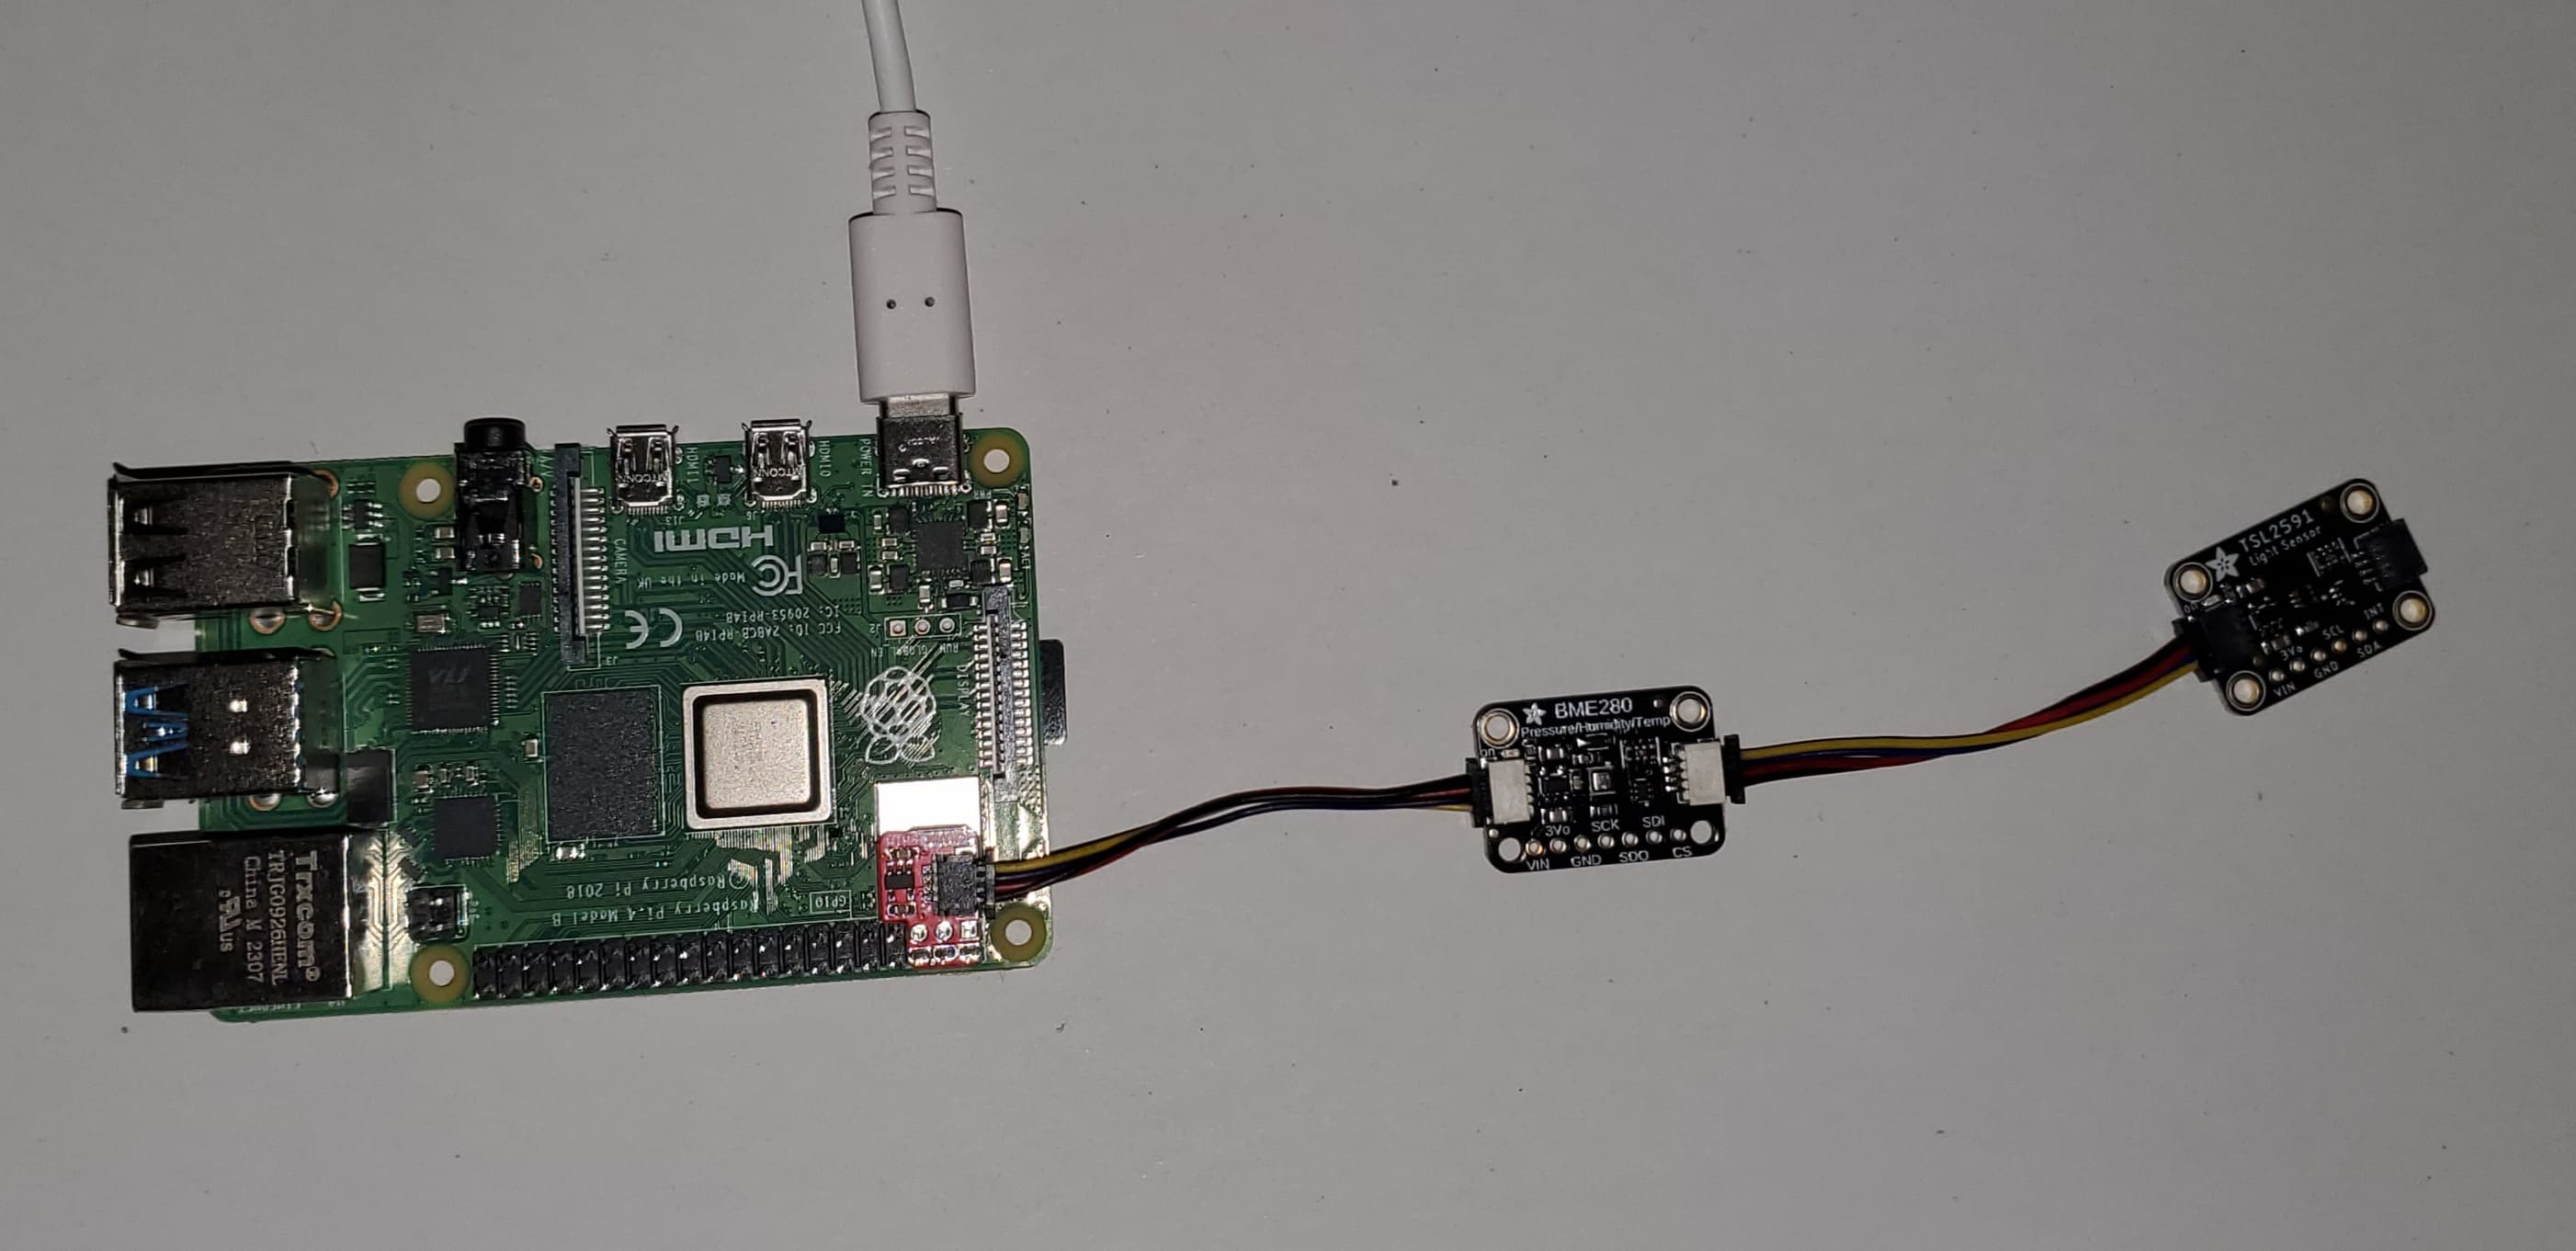
\includegraphics[width=\textwidth]{images/Aufbau.jpg}
	\caption[Aufbau des Prototyps]{Bild des Aufbaus des Prototyps.
		Links ist der Raspberry Pi zu sehen, der als Steuerelement dient.
		Von oben ist der Raspberry Pi mit einem Stromkabel verbunden, das an eine Steckdose angeschlossen ist.
		Rechts sind die beiden Sensoren zu sehen, die hintereinander mit einem Qwiic-Adapter an den Raspberry Pi angeschlossen sind.
	}
	\label{pic:aufbau}
\end{figure}

Der Aufbau des Prototyps ist in \cref{pic:aufbau} dargestellt.
Die Sensoren müssen mit dem Steuerelement verbunden werden, um die Messwerte an das Steuerelement zu übermitteln.
Dafür bieten die Breakout-Boards der Sensoren Qwiic Anschlüsse, die an einen Qwiic-Adapter angeschlossen werden können.
Der Qwiic-Adapter wird an den Raspberry Pi angeschlossen, um die Sensoren mit dem Steuerelement zu verbinden.
So können die Sensoren einfach angeschlossen und betrieben werden, ohne dass eine aufwendige Verkabelung notwendig ist.

Zusammengefasst besteht der Prototyp aus einem Raspberry Pi, der als Steuerelement dient, und zwei Sensoren, die an den Raspberry Pi angeschlossen sind.
Als Kommunikationsschnittstelle wird WLAN verwendet, um mit dem Server zu kommunizieren.
Der erste Sensor ist ein Lichtsensor, der die Lichtintensität misst, und der zweite Sensor ist ein kombinierter Temperatur-, Luftfeuchtigkeits- und Luftdrucksensor, der die Umgebungstemperatur, -luftfeuchtigkeit und -luftdruck misst.
Im nächsten Abschnitt wird die Programmierung des Prototyps beschrieben, um die Funktionalitäten des Prototyps zu realisieren.



\section{Entwicklung des Prototyps}\label{sec:programmierung}
In diesem Abschnitt wird die Entwicklung der Softwarekomponenten des Prototyps beschrieben, die für die Umsetzung des Systems notwendig sind.
Dabei wird das zu realisierende System aus \cref{sec:realisieren} umgesetzt, welches auf der Konzeption basiert.
Zunächst werden die verwendeten Programmiersprachen und Frameworks für die verschiedenen Softwarekomponenten des Systems erläutert.
Anschließend wird die Entwicklung des Definitionsformates für Regeln, Sensoren und externe Datenquellen beschrieben, um die Funktionalitäten des Prototyps zu realisieren.
Daraufhin wird die Entwicklung des Sensor- und Aktuatorkoffers beschrieben, der die zentrale Komponente des Systems darstellt.
Anschließend wird die Entwicklung des Servers beschrieben, der als Bindeglied zwischen dem Sensor- und Aktuatorkoffer und der Nutzerschnittstelle dient.
Zuletzt wird die Entwicklung der Nutzerschnittstelle beschrieben, die für die Darstellung der Sensordaten und die Konfiguration des Systems zuständig ist.


\subsection{Auswahl der Programmiersprachen und Frameworks}
In diesem Abschnitt wird die Auswahl der verwendeten Programmiersprachen und Frameworks für die verschiedenen Softwarekomponenten des Systems erläutert.
Aufgrund der unterschiedlichen Anforderungen und Funktionen des Systems sind die Softwarekomponenten in drei übergreifende Bereiche unterteilt: den Sensor- und Aktuatorkoffer, den Server und die Nutzerschnittstelle.
Diese Trennung ermöglicht es, für jede Komponente die am besten geeigneten Technologien zu verwenden.

Für den Sensor- und Aktuatorkoffer wird die Programmiersprache Python verwendet, da diese eine Vielzahl an Bibliotheken für die Arbeit mit den Schnittstellen des Raspberry Pi zur Interaktion mit den Sensoren bietet.
Weiterhin kann Pythoncode mit leichten Anpassungen zu MicroPython auf Mikrocontrollern wie dem ESP32 oder Arduino portiert werden, was die Flexibilität und Einsatzmöglichkeiten des Systems weiter erhöht.
Weiterhin stellt der Sensor- und Aktuatorkoffer die zentrale Komponente des Systems dar, deren Subkomponenten direkt implementiert werden müssen, sodass die Verwendung eines Frameworks nicht notwendig ist.

Der Server stellt das Bindeglied zwischen dem Sensor- und Aktuatorkoffer und der Nutzerschnittstelle dar und ist für die Speicherung der Sensordaten sowie die Verarbeitung von externen Datenquellen sowie die Verteilung von Benachrichtigungen zuständig.
Der Prototyp setzt für dieses Mitglied auf eine REST-API, die die Kommunikation zwischen den Bereichen sicherstellt.
Dabei wird der Server nur von den anderen Komponenten angesprochen und antwortet auf diese Anfragen, weshalb eine REST-API ausreichend ist.
Für die Implementierung der REST-API wird das Python-Framework Flask\footnote{\href{https://flask.palletsprojects.com/en/latest/}{Flask}} verwendet, da es eine einfache Implementierung der Schnittstelle erlaubt, den Anforderungen des Prototyps entspricht, sowie ein gängiger Standard für solche Anwendungen ist~\cite{FlaskUsage}.

Die Nutzerschnittstelle des Prototyps ist für die Darstellung der Sensordaten und die Konfiguration des Systems zuständig.
Für die Implementierung der Nutzerschnittstelle wird eine Webanwendung verwendet, die im Browser ausgeführt wird.
Diese Webanwendung basiert auf React als Framework, welches die Programmiersprache JavaScript verwendet.
React ist ein gängiges Framework für die Entwicklung von Webanwendungen, das eine Vielzahl von Bibliotheken unterstützt, die für ein Dashboard nützlich sind, wie Graphen zur Darstellung der Sensordaten~\cite{ReactUsage}.

Zusammengefasst wird für den Sensor- und Aktuatorkoffer Python, für den Server Python mit Flask und für die Nutzerschnittstelle JavaScript mit React verwendet.
Im nächsten Abschnitt wird die Entwicklung des Definitionsformates für Regeln, Sensoren und externe Datenquellen beschrieben, um die Funktionalitäten des Prototyps zu realisieren.


\subsection{Entwicklung des Definitionsformats für Regeln, Sensoren und externe Datenquellen}
In diesem Abschnitt wird die Entwicklung eines flexiblen Formats zur Definition von Regeln, Sensoren und externen Datenquellen beschrieben.
Außerdem ist ein Platzhalter für die spätere Integration von Aktuatoren vorgesehen.
Die gewählte Struktur basiert auf JSON, da dieses Format einfach zu lesen und zu erweitern ist.

Für eine einfache und universelle Einsetzbarkeit des gesamten Systems ist es wichtig, dass das System flexibel konfiguriert werden kann und für die Zukunft eine einfache Erweiterung ermöglicht.
Dazu gehört auch, dass die Struktur der Konfiguration logisch und einfach zu verstehen ist, um diesen Zielen nicht im Wege zu stehen.
Das Definitionsformat besteht aus vier Hauptkomponenten: \emph{sensors} (Sensoren), \emph{actors} (Aktuatoren), \emph{external} (externe Datenquellen) und \emph{rules} (Regeln), wobei die Aktuatoren nicht implementiert sind.
Für eine Erweiterung des Systems um Aktuatoren kann das Definitionsformat für die Sensoren als Vorlage dienen.


\begin{figure}[!htb]
\begin{lstlisting}[language=json, caption={[JSON Struktur des Definitionsformates]
	Grundlegende JSON Struktur des Definitionsformates.
	Die Sensoren sind in \cref{lst:sensor-struktur} genauer beschrieben.
	Die Aktuatoren sind nicht implementiert.
	Die externen Datenquellen sind in \cref{lst:external-struktur} genauer beschrieben.
	Die Regeln sind in \cref{lst:rule-struktur} genauer beschrieben.
},
	label={lst:grundlegende-struktur}
]
{
	"sensors": {...},
	"actors": {...},
	"external": {...}
	"rules": {...},
}
\end{lstlisting}
\end{figure}
\begin{figure}[!htb]
\begin{lstlisting}[
	language=json,
	caption={[Struktur der Sensoren im Definitionsformat.]
	Grundlegende Struktur der Sensoren im Definitionsformat.
	Dargestellt sind beispielhaft die zwei Sensoren mit den Schlüsseln \emph{s\_temperature} und \emph{s\_weather}.
	Die Aktionen für einen Sensor des Typs I2C werden in \cref{lst:sensor-aktionen} genauer beschrieben.
	},
	label={lst:sensor-struktur}
]
"sensors": {
	"s_temperature": {
		"name": "Temperature of the shed in degrees Celsius",
		"type": "I2C",
		"i2c_address": "0x77",
		"actions": [...],
		"factor": 0.0095105250,
		"offset": -273.15,
		"msb_first": false
	},
	"s_weather": {
		"name": "Weather",
		"type": "network"
	}
}
\end{lstlisting}
\end{figure}

Jeder Sensor erhält eine eindeutige ID als Schlüssel und kann verschiedenen Typen zugeordnet werden, wie I2C-Sensoren oder Netzwerksensoren.
Diese Struktur ist erweiterbar, sodass in Zukunft weitere Sensortypen hinzugefügt werden können.
Als \emph{type} (Typ) sind für den Prototyp \emph{i2c} (I2C-Sensoren) und \emph{network} (Netzwerksensoren) implementiert, wobei je nach Sensortyp unterschiedliche Informationen benötigt werden.
Für I2C-Sensoren sind etwa die \emph{i2c\_address} (I2C-Adresse), die an den Sensor zu sendenden \emph{actions} (Steuerbefehle), einen \emph{factor} (Korrekturfaktor) einen \emph{offset} (Versatz) für den Messwert, und die Reihenfolge der Datenbytes des Ergebnisses über \emph{msb\_first} erforderlich.
Im Beispiel \cref{lst:sensor-struktur} ist die Definition eines über I2C angeschlossenen Temperatursensors und eines Netzwerksensors dargestellt.
Um den Temperatursensor korrekt anzusteuern, wird seine I2C-Adresse \emph{0x77} benötigt, sowie Steuerbefehle, um ihn zu konfigurieren und Messwerte auszulesen.
Der Temperatursensor gibt die Temperatur in keiner normalen Einheit zurück, diese muss zunächst berechnet werden.
Für eine approximative Berechnung der Temperatur in Grad Celsius wird ein Faktor von \emph{0,0095105250} und ein Versatz von \emph{-273,15} verwendet.
Da der Wert in mehreren Bytes zurückgegeben wird, muss die Reihenfolge der Bytes berücksichtigt werden, was durch \emph{false} für \emph{msb\_first} angegeben wird.
Dabei steht MSB für \emph{Most Significant Byte}, was beschreibt, dass das höchstwertige Byte zuerst übertragen wird.

\begin{figure}[!htb]
\begin{lstlisting}[language=json, caption={[Struktur der Aktionen von Sensoren des Typs I2C im Definitionsformat.]
	Grundlegende Struktur der Aktionen von Sensoren des Typs I2C im Definitionsformat.
	Dargestellt sind beispielhaft die Aktionen für den Sensor \emph{s\_temperature}.
	},
	label={lst:sensor-aktionen}
]
"actions": [
	{
		"type": "write",
		"data": [
			"0xF4",
			"0b00100101"
		],
		"length": 0
	},
	{
		"type": "sleep",
		"data": ["1"],
		"length": 0
	},
	{
		"type": "read",
		"data": [
			"0xFA"
		],
		"length": 2
	}
]
\end{lstlisting}
\end{figure}

Für I2C-Sensoren existieren drei verschiedene Aktionen, die im Beispiel \cref{lst:sensor-aktionen} dargestellt sind.
Hierbei handelt es sich um \emph{write} (Schreibaktionen), \emph{read} (Leseaktionen) und \emph{sleep} (Schlafaktionen).
Aktionen sind in einer Liste aufgelistet, wobei die Aktionen nacheinander ausgeführt werden.

Schreibaktionen haben in den \emph{data} (Daten) die zu sendenden Bytes in hexadezimaler, dezimaler oder binärer Darstellung.
In diesem Beispiel wird der Sensor konfiguriert, indem mit dem ersten Byte das Register des Sensors und mit dem zweiten Byte der Wert für das Register gesetzt wird.
Die \emph{length} (Länge) ist hierbei ungenutzt.

Schlafaktionen haben in den Daten die Zeit in Sekunden, die bis zur nächsten Aktion gewartet werden soll.
Damit kann sichergestellt werden, dass der Sensor genügend Zeit hat, um die Messung durchzuführen.

Leseaktionen senden Daten so wie Schreibaktionen, jedoch wird die \emph{length} (Länge) benötigt, um die Anzahl der Bytes anzugeben, die vom Sensor zurückgegeben werden.
Dieser Sensor ist in der Lage, auch andere Messungen als die Temperatur durchzuführen, die durch unterschiedliche Register definiert sind.
Durch die Leseaktion wird aber nur die Temperatur zurückgegeben, die in zwei Bytes kodiert ist.
Eine Liste von Aktionen endet immer mit genau einer Leseaktion, um die Messwerte des Sensors zu erhalten.

\begin{figure}[!htb]
\begin{lstlisting}[
	language=json,
	caption={[Struktur der externen Datenquellen im Definitionsformat.]
	Grundlegende Struktur der externen Datenquellen im Definitionsformat.
	Dargestellt ist beispielhaft die externe Datenquelle \emph{s\_weather}.
	},
	label={lst:external-struktur}
]
"external": {
	"s_weather": {
		"type": "url",
		"url": "https://api.open-meteo.com/v1/forecast
						?latitude=52.8342444419322
						&longitude=10.704168884802847
						&daily=precipitation_probability_max
						&timezone=Europe%2FBerlin
						&forecast_days=3",
		"keys": ["daily", "precipitation_probability_max"],
		"function": "max",
	}
}
\end{lstlisting}
\end{figure}
	

Auch externe Datenquellen, wie APIs, werden über das Definitionsformat abgebildet.
Jede externe Datenquelle erhält ebenfalls eine eindeutige ID, die mit der ID eines Netzwerksensors übereinstimmt.
Für das Beispiel \cref{lst:external-struktur} wird der Sensor aus \cref{lst:sensor-struktur} verwendet, um die Wetterdaten für den Standort des Sensors zu erhalten.
Für externe Datenquellen sind unterschiedliche \emph{type} (Typen) möglich, wobei für den Prototyp nur \emph{url} umgesetzt ist.
Hierbei handelt es sich bei der angegebenen URL um eine API, die ihre Daten im JSON Format zurückgibt.
Über eine Liste von \emph{keys} (Schlüsseln) kann das zurückgegebene JSON der API durchlaufen werden, um den gewünschten Wert zu erhalten.
Zudem kann eine \emph{function} (Funktion) wie das Maximum einer Liste \emph{max} auf die zurückgegebenen Daten angewendet werden.
In diesem Beispiel gibt die API die Wahrscheinlichkeit für Niederschlag für die nächsten drei Tage zurück, wobei das weiter definiert ist, dass das Maximum dieser Werte als Messwert zurückgegeben wird.
Weitere Typen und Funktionen können in Zukunft hinzugefügt werden, um die Flexibilität des Systems zu erhöhen.

\begin{figure}[!htb]
\begin{lstlisting}[
	language=json,
	caption={[Struktur der Regeln im Definitionsformat.]
	Grundlegende Struktur der Regeln im Definitionsformat.
	Dargestellt ist beispielhaft die Regel \emph{r\_temperature\_low}.
	Die Elemente dieser Beispielregel sind in \cref{lst:rule-notify}, \cref{lst:rule-condition}, \cref{lst:rule-sense} und \cref{lst:rule-send} genauer beschrieben.
	},
	label={lst:rule-struktur}
]
"rules": {
	"r_temperature_low": {
		"name": "Check for low temperature",
		"elements": [...],
		"repeating": true,
		"repeat_interval": 3600
	}
}
\end{lstlisting}
\end{figure}

Auch jede Regel erhält eine eindeutige ID als Schlüssel im Definitionsformat.
Jede Regel besteht aus einem \emph{name} (Namen), einer Liste von \emph{elements} (Elementen), die entweder Bedingungen oder Aktionen sind, über \emph{repeating} ob sie sich wiederholen soll oder nur einmalig ausgeführt wird und einem \emph{repeat\_interval} (Wiederholungsintervall) in Sekunden.
Eine Beispielregel ist in \cref{lst:rule-struktur} dargestellt und wird in den folgenden Paragrafen genauer erläutert.
Diese Regel überprüft, ob die Temperatur zu niedrig ist und benachrichtigt den Benutzer entsprechend.
Dabei wird diese Regel alle 3600 Sekunden wiederholt, um den Benutzer regelmäßig zu informieren.
Die Elemente einer Regel sind eine Liste von Bedingungen und Aktionen, die nacheinander ausgeführt werden.

\begin{figure}[!htb]
\begin{lstlisting}[
	language=json,
	caption={[Struktur einer Aktion vom Typ Benachrichtigung im Definitionsformat.]
		Grundlegende Struktur einer Aktion vom Typ Benachrichtigung im Definitionsformat.
		Dargestellt ist beispielhaft eine Benachrichtigung, die den Benutzer über das Messen der Temperatur informiert.
	},
	label={lst:rule-notify}
]
"elements": [
	{
	"name": "Measuring Temperature",
	"type": "action",
	"action_type": "notify",
	"text": "Measuring temperature",
	"priority": "info"
	},
	{...},
	{...},
	{...}
]
\end{lstlisting}
\end{figure}

Verschiedene Arten von Aktionen sind möglich, wie Benachrichtigungen.
Eine Benachrichtigung ist in \cref{lst:rule-notify} dargestellt und besteht aus einem \emph{name} (Namen), einem \emph{type} (Typ), der in diesem Fall eine Aktion ist, einem \emph{action\_type} (Aktionstyp), der in diesem Fall eine Benachrichtigung ist, einem \emph{text} (Benachrichtigungstext) und einer \emph{priority} (Priorität).
Die Priorität für dieses Beispiel ist \emph{info} und außerhalb dieser JSON-Struktur kann definiert werden, welche Priorität über welchen Benachrichtigungskanal wie E-Mail oder SMS gesendet wird.

\begin{figure}[!htb]
\begin{lstlisting}[
	language=json,
	caption={[Struktur einer Bedingung im Definitionsformat.]
		Grundlegende Struktur einer Bedingung im Definitionsformat.
		Dargestellt ist beispielhaft eine Bedingung, die überprüft, ob die Temperatur über 0 Grad Celsius liegt.
		Der \emph{then} Block ist der Übersichtlichkeit halber nicht dargestellt.
		Eine Aktion des Typs Benachrichtigung ist im \emph{else} Block dargestellt.
	},
	label={lst:rule-condition}
]
"elements": [
	{...},
	{
		"name": "Check temperature level",
		"type": "condition",
		"first_argument": {
			"type": "sensor",
			"argument": "s_temperature",
		},
		"comparison_operator": "greater than",
		"second_argument": {
			"type": "constant",
			"argument": 0,
		},
		"then": [...],
		"else": [
			{
				"name": "Temperature is below freezing",
				"type": "action",
				"action_type": "notify",
				"text": "WARNING: Temperature is below freezing",
				"priority": "high"
			}
		]
	},
	{...},
	{...}
]
\end{lstlisting}
\end{figure}

Neben Aktionen können auch Bedingungen definiert werden, wobei ein Beispiel in \cref{lst:rule-condition} dargestellt ist.
Eine Bedingung beginnt mit einem \emph{name} (Namen) und dem \emph{type} (Typ) \emph{condition} (Bedingung).
Weiterhin werden ein \emph{first\_argument} (erstes Argument) und ein \emph{second\_argument} (zweites Argument) definiert, die über einen \emph{comparison\_operator} (Vergleichsoperator) miteinander verglichen werden.
Die Argumente bestehen aus einem \emph{type} (Typ) und einem \emph{argument} (Argument), wobei für den Prototyp \emph{sensor} (Sensoren) und \emph{constant} (Konstanten) implementiert sind.
Als \emph{argument} für den Sensor wird die ID des Sensors verwendet, während für die Konstante eine Zahl angegeben wird.
Bei Angabe eines Sensorarguments wird zum Zeitpunkt der Ausführung der Regel der entsprechende Sensor über die Sensordefinition angesteuert und ausgelesen.
In diesem Beispiel wird mit dem Vergleichsoperator \emph{greater than} überprüft, ob die Temperatur über 0 Grad Celsius liegt.
Im Falle einer erfüllten Bedingung werden die Elemente in \emph{then} ausgeführt, andernfalls die Elemente in \emph{else}.
Als Elemente sind hier wieder Aktionen und Bedingungen möglich, wodurch eine beliebige Verschachtelung möglich ist, die komplexe Regelablaufläufe ermöglicht.
Hier wird im Falle einer nicht erfüllten Bedingung eine Benachrichtigung mit der Priorität \emph{high} ausgeführt, um den Benutzer zu warnen.

\begin{figure}[!htb]
\begin{lstlisting}[
	language=json,
	caption={[Struktur einer Aktion des Typs Messen im Definitionsformat.]
		Grundlegende Struktur einer Aktion des Typs Messen im Definitionsformat.
		Dargestellt ist beispielhaft eine Aktion, die die Wahrscheinlichkeit für Niederschlag misst.
	},
	label={lst:rule-sense}
]
"elements": [
	{...},
	{...},
	{
		"name": "Sense rain probability",
		"type": "action",
		"action_type": "sense",
		"sensor_id": "s_weather"
	},
	{...}
]
\end{lstlisting}
\end{figure}

Eine weitere Aktion neben Benachrichtigungen ist das Messen von Daten, wie in \cref{lst:rule-sense} dargestellt.
Diese Aktion beginnt mit einem Namen (\emph{name}), einem Typ (\emph{type}) \emph{action}, einem Aktionstyp (\emph{action\_type}) \emph{sense} und der ID des Sensors, der gemessen werden soll (\emph{sensor\_id}).
In diesem Beispiel wird der Netzwerksensor aus \cref{lst:external-struktur} verwendet, um die Wahrscheinlichkeit für Niederschlag zu messen.
Neben der Messung von Sensoren innerhalb von Bedingungen können Messungen auch direkt angestoßen werden.

\begin{figure}[!htb]
\begin{lstlisting}[
	language=json,
	caption={[Struktur einer Aktion des Typs Senden im Definitionsformat.]
		Grundlegende Struktur einer Aktion des Typs Senden im Definitionsformat.
		Dargestellt ist beispielhaft eine Aktion, die die Temperatur und die Wahrscheinlichkeit für Niederschlag sendet.
	},
	label={lst:rule-send}
]
"elements": [
	{...},
	{...},
	{...},
	{
		"name": "Send temperature level",
		"type": "action",
		"action_type": "send",
		"values_to_send": ["s_temperature", "s_weather"],
		"negative_time_offset_start": 8000,
		"negative_time_offset_end": 0
	}
]
\end{lstlisting}
\end{figure}

Die letzte für den Prototyp implementierte Aktion ist das Senden von Daten, wie in \cref{lst:rule-send} dargestellt.
Auch diese Aktion beginnt mit dem Namen, Typen und Aktionstypen, wobei der Aktionstyp \emph{send} ist.
Weiterhin wird eine Liste von Sensor-IDs in \emph{values\_to\_send} angegeben, die gesendet werden sollen.
Zusätzlich kann ein negativer Zeitversatz (\emph{negative\_time\_offset\_start} und \emph{negative\_time\_offset\_end}) angegeben werden, um den Zeitraum festzulegen, in dem die Daten gesendet werden.
In diesem Beispiel werden die Messwerte des Temperatursensors und des Netzwerksensors der letzten 8000 Sekunden an das restliche System gesendet.
Messwerte werden mit einem Zeitstempel gespeichert, sodass Duplikationen herausgefiltert werden können.

Zusammengefasst beschreibt dieser Abschnitt die Entwicklung eines flexiblen und erweiterbaren JSON-basierten Formats zur Definition von Regeln, Sensoren und externen Datenquellen.
Die Struktur ist logisch aufgebaut und ermöglicht eine einfache Erweiterung an allen Stellen wie die Integration von Aktuatoren in der Zukunft.
Sensoren erhalten eindeutige IDs und können je nach Typ, wie I2C oder Netzwerk, spezifische Attribute und Aktionen definieren.
Externe Datenquellen, wie APIs, können ebenfalls eingebunden werden.
Regeln bestehen aus Aktionen und Bedingungen, die flexibel kombiniert werden können, um komplexe Abläufe zu steuern.
Im nächsten Abschnitt wird die Entwicklung des Sensor- und Aktuatorkoffers beschrieben.


\subsection{Entwicklung des Servers}
In diesem Abschnitt wird die Entwicklung des Servers beschrieben, der als Bindeglied zwischen dem Sensor- und Aktuatorkoffer und der Nutzerschnittstelle dient.
Der Server ist für die Speicherung der Sensordaten, die Verarbeitung von externen Datenquellen und die Verteilung von Benachrichtigungen zuständig.
Dabei wird die Implementierung der REST-API, der Benachrichtigungen, der externen Datenquellen und der Datenbank beschrieben.

\subsubsection{Entwicklung der REST-API}
Die REST-API stellt den zentralen Vernetzungspunkt des Systems dar, über den die Kommunikation zwischen den Komponenten stattfindet.
Die API besteht aus sechs Endpunkten, die die Kommunikation zwischen den Komponenten ermöglichen.
Der Endpunkt \emph{/notifications} mit der POST Methode erwartet ein JSON mit einer \emph{message} und einer \emph{priority}, um eine Benachrichtigung an den Benutzer zu senden.
Wird dieser Endpunkt aufgerufen, werden die übergebenen Parameter an die Benachrichtigungskompontente weitergegeben, die diese weiter verarbeitet.
Der Endpunkt \emph{/external/<sensor\_id>} mit der GET Methode erwartet die ID eines Netzwerksensors, gibt diese ID an die Komponente für externe Datenquellen weiter, welche die Daten der externen Datenquelle zurückgibt.
Über den Endpunkt \emph{/measurements} mit der GET Methode können alle in der Datenbank gespeicherten Messwerte abgerufen werden.
Wird dieser Endpunkt mit der POST Methode aufgerufen, werden Messwerte im JSON-Format erwartet, die als Schlüssel die ID des Sensors und als Wert eine Liste von Zeitstempeln und Messwerten enthalten.
Diese werden dann an die Datenbank weitergegeben, um gespeichert zu werden.
Der Endpunkt \emph{/definitions} mit der GET Methode gibt die Konfiguration des Systems zurück, die im Definitionsformat definiert ist.
Der Endpunkt \emph{/definitions} mit der POST Methode erwartet ein JSON mit der Konfiguration des Systems, die im Definitionsformat definiert ist.
Sie wird anschließend in der Datenbank gespeichert.

\subsubsection{Entwicklung der Benachrichtigungen}
Benachrichtigungen sind ein wichtiger Bestandteil des Systems, um den Benutzer über wichtige Ereignisse zu informieren.
Für den Prototyp ist in der Benachrichtigungskomponente ein festes Mapping von Prioritäten auf Benachrichtigungskanäle implementiert.
Basierend auf diesem Mapping werden Benachrichtigungen verarbeitet und spezifische Methoden aufgerufen, die die Benachrichtigungen über den entsprechenden Kanal senden.
Für den Prototyp ist der Benachrichtigungskanal Terminal implementiert, der die Benachrichtigungen auf der Konsole ausgibt.
In Zukunft können weitere Kanäle wie E-Mail oder SMS hinzugefügt werden, indem die entsprechenden Methoden implementiert werden.

\subsubsection{Entwicklung der externen Datenquellen}
Externe Datenquellen erweitern die Möglichkeiten des Systems um mehr als nur direkt angeschlossene Sensoren.
So können etwa Wetterdaten verwendet werden, um das Verhalten des Systems zu steuern.
Für den Prototyp ist der \emph{url}-Typ implementiert, der eine beliebige URL aufrufen kann, die Daten als JSON zurückgibt.
Dafür wird die für den Sensor angegebene URL aufgerufen und das zurückgegebene JSON wird mittels der angegebenen Schlüssel durchlaufen.
Auf das Ergebnis wird die angegebene \emph{function} angewendet, um den Messwert zu erhalten.
Für den Prototyp ist die Funktion \emph{max} implementiert, die das Maximum einer Liste von Werten zurückgibt.
Weitere Typen wie IoT-Sensoren können in Zukunft durch eine Erweiterung des Match-Case-Statements hinzugefügt werden.

\subsubsection{Entwicklung der Datenbank}
Die Datenbank des Servers ist für die Speicherung der von dem Sensor- und Aktuatorkoffer gesendeten Messwerte zuständig.
Somit können die Messwerte über die Nutzerschnittstelle im Dashboard angezeigt werden.
Dafür werden die Daten im Prototyp in einem Python Dictionary gespeichert, das die ID des Sensors als Schlüssel und eine Liste von Zeitstempeln und Messwerten als Wert enthält.
Diese Art der Speicherung ist für den Prototyp ausreichend, sollte jedoch für eine produktive Umgebung durch eine richtige Datenbank ersetzt werden.
Die Datenbank stellt die Methode \emph{merge\_database} zur Verfügung, um die Datenbank mit neuen Messwerten zu aktualisieren, unter Berücksichtigung von Duplikaten.

\subsubsection{Zusammenfassung der Entwicklung des Servers}
Der Server ist das Bindeglied zwischen dem Sensor- und Aktuatorkoffer und der Nutzerschnittstelle.
Er besteht aus der REST-API, der Benachrichtigungskomponente, der externen Datenquellenkomponente und der Datenbank.
Die REST-API besteht aus vier Endpunkten, wobei zwei dieser Endpunkte über sowohl die GET als auch die POST Methode verfügen.
Die Benachrichtigungskomponente ist für die Verarbeitung von Benachrichtigungen zuständig und verfügt für den Prototyp über ein festes Mapping von Prioritäten auf Benachrichtigungskanäle.
Die externe Datenquellenkomponente ist für die Verarbeitung von externen Datenquellen zuständig und kann über den \emph{url}-Typ beliebige URLs aufrufen, die Daten im JSON-Format zurückgeben.
Im nächsten Abschnitt wird die Entwicklung des Sensor- und Aktuatorkoffers beschrieben, der für die Ansteuerung der Sensoren und Aktuatoren zuständig ist.


\subsection{Entwicklung des Sensor- und Aktuatorkoffers}
In diesem Abschnitt wird die Entwicklung der Softwarekomponenten des Sensor- und Aktuatorkoffers beschrieben.
Der Sensor- und Aktuatorkoffer ist für die Ausführung der durch den Nutzer definierten Regeln und der damit verbundenen Ansteuerung der Sensoren und Aktuatoren zuständig.
Er besteht aus der Schnittstelle, den Definitionen, dem Scheduler, dem Regelausführer, der Sensor- und Aktuatorschnittstelle und der Datenbank.

\subsubsection{Entwicklung der Schnittstelle}
Die Schnittstelle des Sensor- und Aktuatorkoffers zum restlichen System besteht aus einer Klasse und mehreren Methoden, um eine Konfiguration zu parsen.
Das \emph{NetworkInterface} wird mit dem Anfang der URL des Servers initialisiert, wie \emph{http://192.168.42.42:65432}.
Die Schnittstelle stellt die Methoden \emph{send\_data}, \emph{request\_data}, \emph{notify} und \emph{get\_definitions} zur Verfügung.
\emph{get\_definitions} sendet eine GET-Anfrage an \emph{/definitions} des Servers, um die Konfiguration des Systems zu erhalten, anschließend zu parsen und für das System zu setzen.
\emph{send\_data} bekommt die zu sendenden Daten übergeben und sendet diese als JSON via der HTTP POST-Methode an \emph{/measurements} des Servers.
\emph{request\_data} sendet eine GET-Anfrage an \emph{/external/<sensor\_id>} des Servers, um die Daten einer externen Datenquelle zu erhalten.
Mittels \emph{notify} können Benachrichtigungen an den Benutzer gesendet werden, wobei diese mittels POST-Methode an \emph{/notifications} des Servers gesendet werden, mit einem JSON, das den Text und die Priorität der Benachrichtigung enthält.

Der Parser stellt die Methode \emph{parse\_definitions} zur Verfügung, die aus der Konfiguration Python Dictionarys erstellt, welche basierend auf den jeweiligen Typen der Sensoren und Regeln die entsprechenden Klassen instanziiert, welche im nächsten Abschnitt beschrieben werden.
Dabei nutzt der Parser auch unterschiedliche Enums, die die möglichen Typen definieren.

\subsubsection{Entwicklung der Definitionen}
Die Definitionen für Regeln, Sensoren und als Platzhalter auch Aktuatoren werden in \emph{Definitions} Python Dictionarys gespeichert.
Um auf diese zuzugreifen, stehen die Methoden \emph{get\_rule}, \emph{get\_sensor} und \emph{get\_actor} zur Verfügung, die jeweils basierend auf der ID die entsprechende Definition zurückgeben.
In einem Enum werden die möglichen Typen von Sensoren definiert, die im Parser verwendet werden.
Hierdurch ist eine einfache Erweiterung um weitere Sensortypen möglich.
Für die unterschiedlichen Sensorarten können jeweils unveränderliche Datenklassen erstellt werden, die von der Basisklasse \emph{SensorDefinition} erben.
Im Falle komplexerer Sensoren, wie I2C-Sensoren, können für die einzelnen Parameter des Sensors eigene Klassen erstellt werden.
In diesem Fall sind die Aktionen für I2C in einer \emph{I2CAction} Klasse definiert.
Somit können auch tiefere Schachtelungen von Parametern innerhalb einer Sensordefinition abgebildet werden.

Regeln werden durch die \emph{RuleDefinition} Klasse abgebildet, wobei Bedingungen und Aktionen selbst durch \emph{RuleCondition} und \emph{RuleAction} Klassen definiert sind.
Hierbei stellt \emph{RuleAction} eine Basisklasse dar, von der die spezifischen Aktionen wie Benachrichtigungen als \emph{RuleActionNotify} oder Messungen als \emph{RuleActionSense} erben.
Für die Argumente einer Bedingung ist die \emph{RuleArgument} Klasse definiert, wobei der Typ des Arguments durch das Enum \emph{ArgumentType} definiert ist.
Auch für den Vergleichsoperator einer Bedingung ist ein Enum \emph{RuleConditionComparisonOperator} definiert.

\subsubsection{Entwicklung des Schedulers}
Der Scheduler ist eine zentrale Komponente des Sensor- und Aktuatorkoffers, die die Ausführung von Regeln startet.
Diese Ausführungen werden auch als Jobs bezeichnet.
Die Schedulerkomponente besteht aus zwei Klassen: der \emph{Scheduler}-Klasse und der \emph{Job}-Klasse.
Die \emph{Scheduler}-Klasse ist für die Verwaltung und Ausführung der Jobs zuständig, während die \emph{Job}-Klasse die Definition eines Jobs repräsentiert.
Ein Job besteht hierbei aus einer Regel-ID, einem Zeitstempel, zu dem der Job ausgeführt werden soll, ob die Regel wiederholt werden soll und einem Wiederholungsintervall.
Außerdem ist eine Funktion definiert, die Jobs zurückgibt, ob ein zeitlich vor einem anderen Job liegt.
Die \emph{Scheduler}-Klasse beinhaltet eine Prioritätswarteschlange, in der die Jobs automatisch nach ihrem Ausführungszeitpunkt sortiert sind.
Angelegt werden Jobs durch die \emph{create\_job}-Methode, die einen neuen Job erstellt und in die Warteschlange einfügt.
Außerdem weist die \emph{Scheduler}-Klasse eine \emph{run}-Methode auf, die Prioritätswarteschlange durchläuft und Jobs ausführt, die ihren Ausführungszeitpunkt erreicht haben.
Für die Ausführung eines Jobs wird die Regel-ID der \emph{execute\_rule}-Methode des Regelausführers übergeben, der im nächsten Abschnitt beschrieben wird.
Außerdem wird ein neuer Job der Prioritätswarteschlange hinzugefügt, wenn eine Regel wiederholt werden soll.

\subsubsection{Entwicklung des Regelausführers}
Der Regelausführer ist ereignisgesteuert und wird durch den Scheduler aufgerufen, um eine Regel auszuführen.
Hierbei wird eine Regel-ID übergeben, die der Regelausführer über die Definitionen zu der Regel auflöst.
Wie schon im Definitionsformat beschrieben, besteht eine Regel aus einer Liste von Elementen, die entweder Bedingungen oder Aktionen sind.
In einer Schleife werden alle Elemente der Regel durchlaufen und nacheinander durch \emph{execute\_elements} ausgeführt, wobei hier basierend auf dem Typ des Elements die entsprechende Methode des Regelausführers aufgerufen wird.
Handelt es sich bei dem Element um eine Bedingung, wird die \emph{execute\_condition}-Methode aufgerufen, die zunächst die beiden Argumente der Bedingung auflöst.
In dieser Methode wird basierend auf dem Typen des jeweiligen Arguments die entsprechende Methode aufgerufen, um den Wert des Arguments zu erhalten.
Für eine Konstante wird der Wert direkt zurückgegeben, während für einen Sensor die Methode \emph{get\_sensor\_value} der Sensor- und Aktuatorschnittstelle aufgerufen wird.
Mögliche weitere Typen von Argumenten wie eine Maximalfunktion über eine Liste von Werten können in Zukunft dem Match-Case\footnote{\href{https://peps.python.org/pep-0634/}{Python Match Case - Structural Pattern Matching}} hinzugefügt werden.
Nachdem die Argumente aufgelöst wurden, wird durch ein weiteres Match-Case der Vergleichsoperator bestimmt und überprüft, ob die Bedingung erfüllt ist.
Entsprechend wird entweder der \emph{then}-Block oder der \emph{else}-Block der Bedingung wieder durch \emph{execute\_elements} ausgeführt.
Handelt es sich bei einem Element um eine Aktion, wird die \emph{execute\_action}-Methode aufgerufen, die mithilfe eines Match-Case-Statements den Aktionstyp bestimmt und die entsprechende Methode aufruft.

\subsubsection{Entwicklung der Sensor- und Aktuatorschnittstelle}
Die Sensor- und Aktuatorschnittstelle ist für die Ansteuerung der Sensoren und Aktuatoren zuständig.
Sie stellt die Methoden \emph{get\_sensor\_value} und \emph{trigger\_actor} zur Verfügung, um Sensoren auszulesen und Aktuatoren zu steuern, wobei die zweite Methode für den Prototyp nicht implementiert ist.
Die Methoden werden mit der Sensor-ID beziehungsweise der Aktuator-ID aufgerufen und geben den Messwert zurück.
Dabei lädt die Methode die jeweilige Definition mittels der ID aus den Definitionen.
Basierend auf dem Typ des Sensors wird mittels eines Match-Case-Statements die typspezifische Methode aufgerufen, um den Messwert zu erhalten.
Für den Prototyp sind I2C-Sensoren und Netzwerksensoren implementiert, wobei für I2C-Sensoren die Methode \emph{\_handle\_i2c} und für Netzwerksensoren die Methode \emph{\_handle\_network\_sensor} aufgerufen wird.
Die Methode \emph{\_handle\_i2c} iteriert über die Aktionen des Sensors und führt diese nacheinander aus.
Das Ergebnis liegt als Bytearray vor, sodass es zunächst basierend auf der Reihenfolge der Bytes zu einer Zahl umgewandelt wird und anschließend der Korrekturfaktor und der Versatz angewendet werden.
Die Methode \emph{\_handle\_network\_sensor} greift auf die Methode \emph{request\_data} der Netzwerkschnittstelle zu, die sich um die Anfrage an die externe Datenquelle kümmert.
Somit ist die Anfrage unabhängig von der Art der Netzwerkkommunikation, die gekapselt in der Netzwerkschnittstelle behandelt wird.

\subsubsection{Entwicklung der Datenbank}
Die \emph{Database}-Klasse ist für die Speicherung der Messwerte zuständig.
Hierbei wird für den Prototyp ein Python-Dictionary verwendet, welches als Schlüssel die jeweilige Sensor-ID und als Wert eine Liste von Tupeln mit Zeitstempel und Messwert enthält.
Für den Prototyp ist ein Dictionary ausreichend, um alle Funktionen abzudecken, die der Prototyp erfüllen soll.
In einer Produktivumgebung sollte jedoch eine Datenbank verwendet werden, um Messwerte über Neustarts des Systems hinaus sicher zu speichern.
Hierbei können weiterhin die gleichen Methoden für den Zugriff verwendet werden, sodass andere Komponenten nicht angepasst werden müssen.
Um Messwerte zu speichern, ist die Methode \emph{store} implementiert, die eine Sensor-ID, einen Zeitstempel und einen Messwert übergeben bekommt und in das Dictionary einfügt.
Für das Abrufen von Messwerten sind die vier Methoden \emph{retrieve\_entry}, \emph{retrieve\_all\_for\_type}, \emph{retrieve\_time\_intervall} und \emph{retrieve\_all} implementiert, die jeweils einen oder mehrere Messwerte zurückgeben.
Hierbei wird in \emph{retrieve\_entry} ein einzelner Messwert anhand der Sensor-ID und des Zeitstempels zurückgegeben, während in \emph{retrieve\_all\_for\_type} alle Messwerte für einen Sensor zurückgegeben werden.
In \emph{retrieve\_time\_intervall} werden alle Messwerte für einen Sensor innerhalb eines Zeitintervalls zurückgegeben und in \emph{retrieve\_all} alle Messwerte für alle Sensoren.

\subsubsection{Zusammenfassung der Entwicklung des Sensor- und Aktuatorkoffers}
Zusammengefasst besteht der Sensor- und Aktuatorkoffer aus der Schnittstelle, den Definitionen, dem Scheduler, dem Regelausführer, der Sensor- und Aktuatorschnittstelle und der Datenbank.
Die Schnittstelle ist für die Kommunikation mit dem restlichen System zuständig und stellt Methoden zur Verfügung, um die Konfiguration zu parsen.
Die Definitionen enthalten die Definitionen für Regeln, Sensoren und Aktuatoren, die in Python Dictionarys gespeichert sind.
Der Scheduler verwaltet die Jobs, die aus Regeln und Zeitpunkten bestehen und löst deren Ausführung aus.
Der Regelausführer führt die Regeln aus, indem er die Elemente der Regeln durchläuft und nacheinander ausführt.
Die Sensor- und Aktuatorschnittstelle ist für die Ansteuerung der Sensoren und Aktuatoren zuständig und stellt Methoden zur Verfügung, um Sensoren auszulesen.
Die Datenbank ist für die Speicherung der Messwerte zuständig und stellt Methoden zur Verfügung, um Messwerte abzurufen.
Im nächsten Abschnitt wird die Entwicklung der Nutzerschnittstelle beschrieben, die für die Konfiguration des Systems und die Anzeige der Messwerte zuständig ist.


\subsection{Entwicklung der Nutzerschnittstelle}
In diesem Abschnitt wird die Entwicklung der Nutzerschnittstelle beschrieben, die für die Konfiguration des Systems und die Anzeige der Messwerte zuständig ist.
Die Nutzerschnittstelle besteht aus dem Konfigurationswerkzeug und dem Dashboard, die beide in React implementiert sind.

\subsubsection{Entwicklung des Konfigurationswerkzeugs}

\begin{figure}[!htbp]
	\centering
	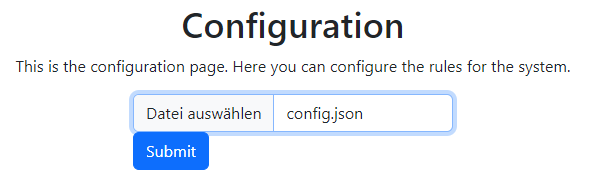
\includegraphics[width=\textwidth]{images/Konfiguration.png}
	\caption[Konfigurationswerkzeug des Prototyps]{
		Screenshot des Konfigurationswerkzeugs des Prototyps.
	}
	\label{pic:konfiguration}
\end{figure}

Das Konfigurationswerkzeug ist ein zentrales Element der Nutzerschnittstelle, um das System zu konfigurieren.
Das Konfigurationswerkzeug des Prototyps ist in \cref{pic:konfiguration} abgebildet, wo zu sehen ist, dass das Konfigurationswerkzeug aus einem Dateiwähler besteht, der es ermöglicht, die Konfiguration im JSON Definitionsformat vom Dateisystem zu laden.
Die geladene Konfiguration wird anschließend mittels des \emph{Submit} Buttons an den POST Endpunkt \emph{/definitions} des Servers gesendet, um die Konfiguration zu setzen.
Realisiert ist das Konfigurationswerkzeug als einzelne React-Komponente \emph{ConfigurationInput}, die den Dateiwähler und die Logik zum Senden der Konfiguration enthält.

\subsubsection{Entwicklung des Dashboards}

\begin{figure}[!htbp]
	\centering
	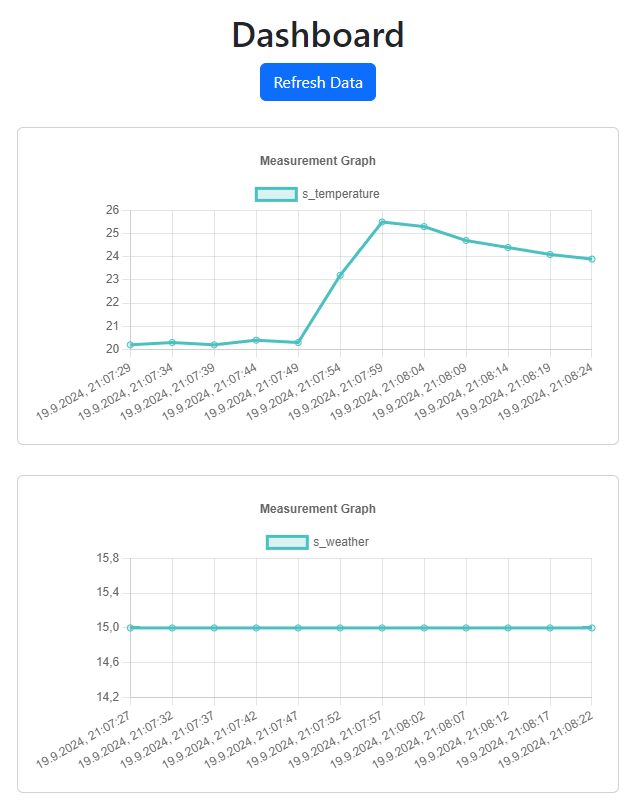
\includegraphics[width=0.95\textwidth]{images/Dashboard.png}
	\caption[Dashboard des Prototyps]{
		Screenshot des Dashboards des Prototyps.
		Abgebildet sind die Diagramme für die Messwerte Temperatur und Regenwahrscheinlichkeit.
	}
	\label{pic:dashboard}
\end{figure}

Das Dashboard ist ein weiteres zentrales Element der Nutzerschnittstelle, um die Messwerte des Systems anzuzeigen.
Es ist in \cref{pic:dashboard} abgebildet, wo zu sehen ist, dass das Dashboard aus Diagrammen besteht, die die Messwerte der Sensoren anzeigen.
Für den Prototyp werden die unterschiedlichen Messwerte jeweils in einem eigenen Diagramm angezeigt, welches mithilfe der \emph{Chart.js}\footnote{\href{https://www.chartjs.org/}{Chart.js}} Bibliothek erstellt wird.
Hierbei werden zwei unterschiedliche React Komponenten verwendet, um das Dashboard zu realisieren.
Die \emph{SingleGraph} Komponente bekommt die Daten für ein einzelnes Diagramm übergeben und ist dafür zuständig, dieses Diagramm mittels \emph{Chart.js} zu erstellen.
Dabei wird die x-Achse als Zeitachse mit den jeweiligen Zeitstempeln und die y-Achse als Messwertachse definiert.
Dies ist im Beispiel ersichtlich, wo der erste Graph die Temperatur in Celsius auf der y-Achse anzeigt und die Zeit als Datums- und Uhrzeitangabe auf der x-Achse.
Dabei wird jede Messung als einzelner Punkt im Diagramm dargestellt, welche durch Linien verbunden sind.
Die Konfiguration, die dieses Beispiel erzeugt hat, ist auf ein Intervall von fünf Sekunden für beide Sensoren eingestellt.
In diesem Beispiel ist auch der zweite Graph zu sehen, der die Wahrscheinlichkeit für Niederschlag in Prozent auf der y-Achse anzeigt.

Die \emph{AllGraphs} Komponente hat einen Button, welcher die Daten für alle Sensoren mittels GET an den Endpunkt \emph{/measurements} des Servers abruft und für jeden Sensor ein \emph{SingleGraph} Diagramm erstellt.
Außerdem ist die Webseite so entwickelt, dass sich die Diagramme automatisch an die Größe des Bildschirms anpassen, sodass sie auch auf mobilen Geräten lesbar sind.

\subsubsection{Zusammenfassung der Entwicklung der Nutzerschnittstelle}
Zusammengefasst besteht die Nutzerschnittstelle aus dem Konfigurationswerkzeug und dem Dashboard, die beide in React implementiert sind.
Das Konfigurationswerkzeug ermöglicht das Laden und Setzen der Konfiguration im JSON-Definitionsformat.
Das Dashboard zeigt die Messwerte des Systems in Diagrammen an, wobei für jeden Sensor ein eigenes Diagramm erstellt wird.


\subsection{Zusammenfassung der Entwicklung des Prototyps}
Zusammengefasst besteht der Prototyp aus mehreren Komponenten sowie einem Definitionsformat, das die Konfiguration des Systems definiert.
Das Definitionsformat ermöglicht es dem Nutzer, Sensoren, Regeln und externe Datenquellen zu definieren.
Diese Regeln können Bedingungen und Aktionen enthalten, wodurch komplexe Abläufe gesteuert werden können.
Die Sensoren können unterschiedliche Typen haben, wie I2C oder Netzwerk, und spezifische Attribute und Aktionen definieren.
Externe Datenquellen können über das Definitionsformat eingebunden werden.

Der Server ist für die Speicherung der Sensordaten, die Verarbeitung von externen Datenquellen und die Verteilung von Benachrichtigungen zuständig.
Außerdem ist er das Bindeglied zwischen dem Sensor- und Aktuatorkoffer und der Nutzerschnittstelle.
Die REST-API des Servers ermöglicht die Kommunikation zwischen den Komponenten.

Der Sensor- und Aktuatorkoffer ist für die Ausführung der durch den Nutzer definierten Regeln und der damit verbundenen Ansteuerung der Sensoren und Aktuatoren zuständig.
Durch laden der Konfiguration kann er die definierten Regeln ausführen und die Sensoren auslesen.

Die Nutzerschnittstelle ist für die Konfiguration des Systems und die Anzeige der Messwerte zuständig.
Das Konfigurationswerkzeug ermöglicht das Laden und Setzen der Konfiguration im JSON-Definitionsformat.
Das Dashboard zeigt die Messwerte des Systems in Diagrammen an.



\section{Zusammenfassung der Implementierung}
Zusammengefasst wurde in diesem Kapitel die Implementierung des Prototyps beschrieben.
Der Prototyp besteht aus einem Hardware- und einem Softwareteil, die jeweils in mehrere Komponenten unterteilt sind.
Der Hardwareteil besteht aus einem Raspberry Pi, der als zentrale Steuereinheit dient, und Sensoren, die an den Raspberry Pi angeschlossen sind.
Der Softwareteil besteht aus dem Server, der die Kommunikation zwischen den Komponenten ermöglicht, dem Sensor- und Aktuatorkoffer, der für die Ausführung der Regeln und die Ansteuerung der Sensoren und Aktuatoren zuständig ist, und der Nutzerschnittstelle, die für die Konfiguration des Systems und die Anzeige der Messwerte zuständig ist.
Die Implementierung des Prototyps erfolgte in Python und JavaScript, wobei für die Kommunikation zwischen den Komponenten eine REST-API verwendet wird.
Im nächsten Kapitel wird der Prototyp evaluiert, wobei ein Fokus auf die Erfüllung der Anforderungen und dem Mehrwert des Systems gegenüber bestehenden Systemen gelegt wird.

	% !TEX root = ../thesis.tex
\chapter{Evaluation}\label{ch:evaluation}
In diesem Kapitel wird zunächst der entwickelte Prototyp im Hinblick auf die gestellten Anforderungen evaluiert.
Dabei wird für jede Anforderung evaluiert, ob diese durch den Prototyp erfüllt wurde oder nicht und gegebenenfalls, warum dies der Fall ist.
Anschließend wird der Prototyp mit weiteren Lösungsansätzen anhand der Metriken Preis, Energieeffizienz und Skalierbarkeit verglichen.



\section{Evaluation des Prototyps im Hinblick auf die gestellten Anforderungen}
In diesem Abschnitt wird der entwickelte Prototyp im Hinblick auf die gestellten Anforderungen evaluiert.
Dafür wird zunächst für die funktionalen und nicht funktionalen Anforderungen evaluiert, ob diese durch den Prototyp erfüllt werden oder nicht.
Anschließend wird bewertet, ob die Abweichungen von den Anforderungen auf das Konzept zurückzuführen sind oder nicht.


\subsection{Erfüllung der funktionalen Anforderungen}
In diesem Abschnitt wird erläutert, welche funktionalen Anforderungen durch den Prototyp erfüllt wurden und welche nicht.
Die funktionalen Anforderungen sind die Möglichkeit zur Messung, Konfiguration, Regeldefinition, Darstellung der Messdaten in einem Dashboard, Steuerung von Aktuatoren, autonomen Betrieb des Systems und Benachrichtigung des Nutzers.
Dafür wird für jede funktionale Anforderung zunächst kurz beschrieben, was diese bedeutet und wie sie im Prototyp umgesetzt wurde.
Anschließend wird bewertet, ob die Anforderung erfüllt ist oder nicht und gegebenenfalls, warum dies der Fall ist.

Die erste funktionale Anforderung ist die Messung von Umweltdaten, wofür Sensoren universell unterstützt werden sollen.
Der Prototyp unterstützt beispielhaft alle Sensoren, die eine I2C-Schnittstelle aufweisen, wobei exemplarisch ein Lichtsensor TSL2591 und ein Temperatur-, Feuchtigkeits- und Drucksensor BME280 verwendet wurden.
Die Sensoren werden über die I2C-Schnittstelle an den Raspberry Pi angeschlossen und über die Konfiguration des Systems eingebunden.
In der Konfiguration wird die I2C-Adresse des Sensors sowie eine Liste von Aktionen eingetragen, wobei als Aktionen Lesen, Schreiben und Schlafen möglich sind.
Eine Schreib-Aktion beinhaltet eine Liste von Steuerbefehlen, die an den Sensor gesendet werden, um diesen beispielsweise zu konfigurieren oder eine Messung zu starten.
Diese Steuerbefehle enthalten im Normalfall die Adresse des Registers des Sensors, das beschrieben werden soll, sowie den Wert, der in das Register geschrieben werden soll.
Auch Lese-Aktionen enthalten diese Steuerbefehle, wobei hier meist das zu lesende Register angegeben wird.
Außerdem enthält die Lese-Aktion die Anzahl der Bytes, die gelesen werden sollen, sowie die Reihenfolge der Bytes.
Die Schlaf-Aktion ist eine Wartezeit, die der Sensor- und Aktuatorkoffer zwischen zwei Aktionen wartet, da der Sensor beispielsweise bei Messungen eine gewisse Zeit benötigt, bevor er das Ergebnis bereitstellt.
Da das I2C-Protokoll nur Lesen und Schreiben unterstützt, bildet das System mit der Unterstützung von Wartezeiten alle Möglichkeiten der Interaktion mit I2C-Sensoren ab und ist somit universell einsetzbar.
Neben I2C-Sensoren werden im Prototyp auch externe Datenquellen in Form von HTTP-APIs unterstützt, wenn diese eine JSON-Antwort liefern.
Hierfür wird durch die Angabe einer Liste von Schlüsseln und einer Auswertungsfunktion gewährleistet, dass die Antwort navigiert und ausgewertet werden kann.
Somit ist diese Anforderung erfüllt.

Die zweite funktionale Anforderung ist die Möglichkeit, das System als Nutzer selbst konfigurieren zu können.
Der Raspberry Pi verfügt über verschiedene GPIO-Pins, die unterschiedlich verwendet werden können und frei liegen.
Dadurch ist es dem Nutzer möglich, selbst Sensoren und bei einer Erweiterung auch Aktuatoren anzuschließen.
Um diese vollständig in das System zu integrieren, müssen sie in der Konfiguration des Systems eingetragen werden, was im vorherigen Absatz bereits beschrieben wurde.
Dort wurde auch beschrieben, dass nicht nur physische Sensoren, sondern auch externe Datenquellen in das System integriert werden können.
Ein weiterer Aspekt von Konfigurierbarkeit ist Skalierbarkeit, also die Möglichkeit, das System um weitere Sensoren und Aktuatoren zu erweitern und das System großflächig einzusetzen.
Hierbei kann das System auf zwei Arten skaliert werden, zum einen durch die Anzahl der Sensoren und Aktuatoren, die an den Sensor- und Aktuatorkoffer angeschlossen werden, und zum anderen durch die Anzahl der Sensor- und Aktuatorkoffer, die an den Server angeschlossen werden.
Die erste Art der Skalierung ist durch die Anzahl der Pins des Raspberry Pi begrenzt, kombiniert mit den Grenzen der integrierten Protokolle.
Der für den Prototyp verwendete Raspberry 4 Modell B verfügt über 40 GPIO-Pins, wobei einige Protokolle mehrere Pins benötigen, wie I2C, das zwei Pins benötigt.
Als Bus Protokoll unterstützt I2C mehrere Geräte, wodurch die Anzahl der angeschlossenen Geräte aufgrund der 7 Bit Adressierung und einiger reservierter Adressen auf maximal 112 Geräte begrenzt ist, wobei physische Limitierungen wie die Kabellänge und Spannungsprobleme die Anzahl der Geräte (Sensoren und Aktuatoren) weiter einschränken.
Gleichzeitig können nur wenige Geräte über den Raspberry Pi selbst mit Strom versorgt werden, weshalb bei mehreren Geräten oder Geräten mit hohem Stromverbrauch eine externe Stromversorgung für diese notwendig wird.
Die zweite Art der Skalierung ist durch die Kapazität des Servers begrenzt, Anfragen zu beantworten.
In einem Test auf den Messdatenendpunkt des Servers wurden 1000 Anfragen, die jeweils eine Messung enthielten, in 17,6 s verarbeitet.
Dabei wurden die Anfragen von einem Raspberry Pi im gleichen LAN gesendet, was einem realistischen Einsatz des Systems entspricht.
Das entspricht etwa 56,8 Anfragen pro Sekunde, was bedeutet, dass mehr als 50 Sensor- und Aktuatorkoffer, die jede Sekunde eine Messung senden, den Server nicht überlasten würden.
Beide Arten der Skalierbarkeit sind für realistische Anwendungsfälle ausreichend, womit die Konfigurierbarkeit des Systems gegeben ist.

Die dritte funktionale Anforderung ist die Möglichkeit, komplexe Regeln zu definieren.
Der Prototyp ermöglicht dies über ein Definitionsformat, das in einer JSON-Datei abgelegt wird.
In dieser Definition werden die Sensoren, Regeln und externen Datenquellen definiert, wobei ein Platzhalter für die Aktuatoren vorgesehen ist.
Die Definition der Sensoren, Aktuatoren und externen Datenquellen ist notwendig, um diese in den Regeln verwenden zu können.
Die Definition von Sensoren und externen Datenquellen wurde bereits bei der Messung angerissen, weshalb hier nur die Definition von Regeln betrachtet wird.
Eine Regel besteht aus einer Liste von Aktionen und Bedingungen, wobei es als Aktion Messungen, Benachrichtigungen und Senden der Messdaten implementiert ist.
Eine Bedingung besteht aus einem Vergleich von zwei Werten, wobei die Werte Messungen oder Konstanten sein können.
Als Vergleichsoperatoren sind \emph{Gleichheit}, \emph{Größer}, \emph{Kleiner}, \emph{Größer oder gleich} und \emph{Kleiner oder gleich} implementiert.
Hierbei können die Sensoren und Aktuatoren des Systems eingebunden werden, wodurch die Regeln auf die Messdaten reagieren können.
Im Dann oder Sonst Fall einer Regel wird wiederum eine Liste von Aktionen ausgeführt, wodurch die Regeln beliebig komplex gestaltet werden können.
Durch diese Regeldefinitionsmöglichkeit des Systems ist diese Anforderung erfüllt.

Die vierte funktionale Anforderung ist die Darstellung der Messdaten in einem Dashboard.
Hierfür ist im Prototyp eine Webseite implementiert, die über einen Browser aufgerufen wird und die Daten der Sensoren in Diagrammen darstellt.
Diese Diagramme stellen den Zeitverlauf der Messdaten dar, wobei auf der x-Achse die Zeit und auf der y-Achse die Messwerte dargestellt werden.
Dementsprechend ist die Anforderung erfüllt.

Die fünfte funktionale Anforderung ist die Steuerung von Aktuatoren.
Diese Anforderung wurde im Prototyp nicht umgesetzt, weshalb sie nicht erfüllt ist.

Die sechste funktionale Anforderung ist der autonome Betrieb des Systems.
Diese Anforderung wurde im Prototyp nicht umgesetzt, weshalb sie nicht erfüllt ist.

Die letzte funktionale Anforderung ist die Benachrichtigung des Nutzers.
Der Prototyp implementiert eine rudimentäre Benachrichtigungsfunktion, die als einzigen Benachrichtigungskanal das Terminal des Servers unterstützt.
Da keine weiteren Benachrichtigungskanäle oder der Herzschlag implementiert sind, ist diese Anforderung nur teilweise erfüllt.

\begin{table}[!htbp]
	\centering
	\caption[Erfüllung der funktionalen Anforderungen durch den Prototyp.]{
		Übersicht über die Erfüllung der funktionalen Anforderungen durch den Prototyp.
		Zusätzlich sind die von dem Konzept und dem zu realisierenden System erfüllten Anforderungen aufgelistet.
		Die jeweils erfüllten funktionalen Anforderungen sind mit einem Häkchen markiert.
		In einigen Fällen ist eine Anforderung nur teilweise erfüllt, in diesen Fällen ist ein Fragezeichen markiert.
		Nicht erfüllte Anforderungen werden durch ein Kreuz markiert.
	}\label{tab:prototyp-f-anforderungen}
	\begin{tabular}{llll}
		Anforderung			& Konzept	& zu realisierendes System	& Prototyp \\\hline
		Messung				& \OK		& \OK						& \OK \\
		Konfiguration		& \OK		& \OK						& \OK \\
		Regeldefinition		& \OK		& \OK						& \OK \\
		Dashboard			& \OK		& \OK						& \OK \\
		Steuerung			& \OK		& \NO						& \NO \\
		Autonomer Betrieb	& \OK		& \NO						& \NO \\
		Benachrichtigung	& \OK		& \UN						& \UN
	\end{tabular}
\end{table}

Zusammengefasst ist die Erfüllung der funktionalen Anforderungen durch den Prototyp in \cref{tab:prototyp-f-anforderungen} dargestellt.
Dabei sind die Anforderungen Messung, Konfiguration, Regeldefinition und Dashboard erfüllt, während die Anforderungen Steuerung und autonomer Betrieb nicht erfüllt sind und die Benachrichtigung nur teilweise erfüllt ist.
Dem sind die Anforderungen des zu realisierenden Systems gegenübergestellt, wodurch ersichtlich wird, dass der Prototyp die vorher gesteckten Ziele für die funktionalen Anforderungen erreicht hat.



\subsection{Erfüllung der nicht funktionalen Anforderungen}
In diesem Abschnitt wird erläutert, welche der nicht funktionalen Anforderungen durch den Prototyp erfüllt wurden und welche nicht.
Die nicht funktionalen Anforderungen sind der Preis, der Schutz vor den Elementen, die Nutzerfreundlichkeit der Bedienung, die Sicherheit, der sparsame Energieverbrauch, die Verfügbarkeit des Systems, die einfache Wartbarkeit und die visuelle Unauffälligkeit.
Dafür wird für jede nicht funktionale Anforderung zunächst kurz beschrieben, was diese bedeutet und wie sie im Prototyp umgesetzt wurde.
Anschließend wird bewertet, ob die Anforderung erfüllt ist oder nicht und gegebenenfalls, warum dies der Fall ist.

\begin{table}[!htbp]
	\centering
	\caption[Preise aller genutzten Komponenten für den Prototyp.]{
		Tabelle der Preise aller genutzten Komponenten für den Prototyp.\footnotemark
		Außerdem ist der Preis für den Prototyp ohne Sensoren und Sensorzubehör aufgelistet, da diese optional sind.
	}\label{tab:prototyp-preis}
	\begin{tabular}{lr}
		Bauteil & Preis \\\hline
		Raspberry Pi 4 Modell B mit 4 GB RAM					&  58,99 € \\
		Raspberry Pi Netzteil									&   7,79 € \\
		32 GB microSD Speicherkarte								&   5,75 € \\
		Lichtsensor - TSL2591									&   8,80 € \\
		Temperatur-, Feuchtigkeits- und Drucksensor - BME280	&  18,60 € \\
		Qwiic SHIM Header										&   1,30 € \\
		2 * 50 mm Qwiic											&   2,30 € \\\hline
		Summe ohne Sensoren und Sensorzubehör					&  72,53 € \\
		Gesamtsumme												& 103,53 € \\
	\end{tabular}
\end{table}

\footnotetext{Preise von \href{https://www.rasppishop.de/}{Rasppishop}, \href{https://www.berrybase.de}{BerryBase} und \href{https://www.reichelt.de/}{reichelt}, Stand 2024-09-22, inklusive Umsatzsteuer, zuzüglich Versandkosten}

Die wichtigste nicht funktionale Anforderung des Systems ist der Preis, da das System für den Einsatz von Hobbygärtnern konzipiert ist.
Der entwickelte Prototyp besteht aus einem Raspberry Pi 4 Modell B mit 4 GB RAM, einem Netzteil, einer SD-Karte, zwei Sensoren, einem Qwiic Shim Header und zwei Qwiic Kabeln.
Die Preise der Bauteile sind in \cref{tab:prototyp-preis} aufgelistet und ergeben eine Gesamtsumme von 103,53~€, oder 72,53~€ ohne Sensoren und Sensorzubehör.
Primärer Kostenfaktor ist der Raspberry Pi, der mehr als die Hälfte der Gesamtkosten ausmacht, weshalb bei Verwendung eines Mikrocontrollers wie dem ESP32, welcher ab 6,80 € erhältlich ist\footnote{Preis von \href{https://www.berrybase.de}{BerryBase}, Stand 2024-09-22, inklusive Umsatzsteuer, zuzüglich Versandkosten}, die Kosten deutlich reduziert werden können.
Nicht einbezogen sind die Kosten für den Server, der die Daten speichert und die Webseite mit der Konfiguration und dem Dashboard bereitstellt sowie laufenden Kosten für den Betrieb des Systems.
Außerdem sind die Kosten nicht berücksichtigt, die für eine Erfüllung der bisher nicht erfüllten Anforderungen notwendig wären.
Insgesamt befinden sich die Kosten im niedrigen dreistelligen Bereich, was aufgrund einer hohen Ausgabebereitschaft von Hobbygärtnern ein akzeptabler Preis ist~\cite{AusgabebereitschaftGarten}

Die zweite nicht funktionale Anforderung ist der Schutz vor den Elementen, da das System im Außenbereich eingesetzt wird.
Der Prototyp weist keinerlei Gehäuse auf, weshalb er nicht vor den Elementen geschützt ist und daher nicht im Außenbereich eingesetzt werden kann.

Die dritte nicht funktionale Anforderung ist die Nutzerfreundlichkeit der Bedienung, da das System von Hobbygärtnern bedient wird.
Zur Nutzung des Systems müssen zunächst der Server, die Webseite und die Steuerung des Sensor- und Aktuatorkoffers auf dem Raspberry Pi gestartet werden, wofür ein rudimentäres Verständnis von Kommandozeilenbefehlen notwendig ist.
Die Nutzerschnittstelle des Prototyps besteht aus einer Webseite, die über einen Browser aufgerufen wird, auf der über ein Dashboard die Daten dargestellt und über ein Konfigurationswerkzeug das System konfiguriert werden kann.
Hierbei ist die Bedienung des Dashboards intuitiv, da es als Interaktionsmöglichkeit lediglich einen Button gibt, der die aktuellen Daten des Systems abruft.
Ansonsten stellt das Dashboard die Daten für die verschiedenen Sensoren in Diagrammen dar, die die Werte über die Zeit anzeigen.
Somit ist die Bedienung des Dashboards für Hobbygärtner einfach und intuitiv.
Die Konfiguration des Systems ist jedoch nicht intuitiv, da die Konfiguration über eine JSON-Datei erfolgt, die manuell bearbeitet werden muss.
Hierbei ist ein rudimentäres Verständnis von JSON-Dateien notwendig, um die Konfiguration durchzuführen.
Eine besondere Herausforderung stellt die Einbindung von Sensoren dar, da in der Konfiguration Steuerbefehle eingetragen werden müssen, mit denen die Sensoren angesprochen werden.
Diese Steuerbefehle sind normalerweise in der Dokumentation des Sensors zu finden, diese Dokumentation ist jedoch nicht immer einfach verständlich.
Somit ist die Konfiguration des Systems für Hobbygärtner nicht intuitiv, weshalb diese Anforderung nur teilweise erfüllt ist.

Die vierte nicht funktionale Anforderung ist die Sicherheit, worunter der Datenschutz, die Datenintegrität und die Angriffssicherheit fallen.
Diese Anforderung bezieht sich primär auf den Datenverkehr zwischen den Komponenten des Systems, da ansonsten ein physischer Zugriff auf das System notwendig ist.
Der Datenverkehr läuft über die REST-Schnittstelle des Servers, die das HTTP-Protokoll nutzt und dementsprechend unverschlüsselt ist.
Daher sind weder der Datenschutz noch die Datenintegrität gewährleistet, da die Daten von Dritten abgefangen und manipuliert werden können.
Gleichzeitig ist die Angriffssicherheit gewährleistet, da für den Prototyp keine Aktuatorik implementiert ist, die von Dritten manipuliert werden könnte.
Somit ist die Anforderung nur teilweise erfüllt.

Die fünfte nicht funktionale Anforderung ist der sparsame Energieverbrauch, da das System auch im Batteriebetrieb betrieben werden können soll.
Ein Raspberry Pi 4 Modell B verbraucht im Betrieb zwischen 2,7 Watt im Leerlauf und 6,5 Watt unter Last~\cite{RaspberryPi4Power}.
Dabei sind die Sensoren vernachlässigbar, so verbraucht der Lichtsensor TSL2591 im Betrieb 0,001 Watt~\cite{TSL2591}.
Bei einem Strompreis von 0,25 € pro Kilowattstunde ergeben sich Kosten von 5,90 € bis 14,20 € pro Jahr.
Wird das System beispielsweise mit einem 20 Ah Akku mit einer Nennspannung von 3,7 Volt betrieben, so ergibt sich eine Laufzeit zwischen 27,4 Stunden und 11,4 Stunden, abhängig von der Auslastung des Systems.
Somit ist diese Anforderung nicht erfüllt.

Die sechste nicht funktionale Anforderung ist die Verfügbarkeit des Systems, welche meint, dass das System jederzeit verfügbar sein oder im Fehlerfall den Nutzer informieren soll.
Um sicherzustellen, dass der Nutzer informiert wird, ist in der Konzeption ein Herzschlag vorgesehen, dessen Ausfall eine Benachrichtigung an den Nutzer auslöst.
Da dieser Herzschlag für den Prototyp nicht umgesetzt wurde, ist diese Anforderung für den Prototyp nicht erfüllt.

Die siebte nicht funktionale Anforderung ist die einfache Wartbarkeit, da das System von Hobbygärtnern gewartet werden soll.
Der Prototyp besteht aus wenigen Komponenten, die mittels Steckverbindungen verbunden sind, weshalb die Komponenten im Fehlerfall von Hobbygärtnern selbst getauscht werden können.
Daher ist diese Anforderung erfüllt.

Die letzte nicht funktionale Anforderung ist die visuelle Unauffälligkeit, damit das System im Garten nicht stört.
Der Prototyp besteht aus wenigen Komponenten, die ohne Akku oder Ladekabel etwa eine Fläche von $80$ $cm^2$ einnehmen, weshalb das System selbst bei einer Integration eines Gehäuses mit Akku nur einen geringen Platzbedarf hat.
Somit ist diese Anforderung erfüllt.


\begin{table}[!htbp]
	\centering
	\caption[Erfüllung der nicht funktionalen Anforderungen durch den Prototyp.]{
		Übersicht über die Erfüllung der nicht funktionalen Anforderungen durch den Prototyp.
		Zusätzlich sind die von dem zu realisierenden System erfüllten Anforderungen aufgelistet.
		Die jeweils erfüllten nicht funktionalen Anforderungen sind mit einem Häkchen markiert.
		In einigen Fällen ist eine Anforderung nur teilweise erfüllt, in diesen Fällen ist ein Fragezeichen markiert.
		Nicht erfüllte Anforderungen werden durch ein Kreuz markiert.
	}\label{tab:prototyp-nf-anforderungen}
	\begin{tabular}{lll}
		Anforderung			& zu realisierendes System	& Prototyp \\\hline
		Preis				& \OK						& \OK \\
		Elementschutz		& \NO						& \NO \\
		Nutzerfreundlichkeit& \NO						& \UN \\
		Sicherheit			& \NO						& \UN \\
		Energieverbrauch	& \NO						& \NO \\
		Verfügbarkeit		& \NO						& \NO \\
		Wartbarkeit			& \NO						& \OK \\
		Unauffälligkeit		& \NO						& \OK 
	\end{tabular}
\end{table}

Zusammengefasst ist die Erfüllung der nicht funktionalen Anforderungen durch den Prototyp in \cref{tab:prototyp-nf-anforderungen} dargestellt.
Dabei sind die Anforderungen Preis, Wartbarkeit und Unauffälligkeit erfüllt, während die Anforderungen Elementschutz, Energieverbrauch und Verfügbarkeit nicht und die Anforderungen Nutzerfreundlichkeit und Sicherheit nur teilweise erfüllt sind.
Dem sind die Anforderungen des zu realisierenden Systems gegenübergestellt, wodurch ersichtlich wird, dass der Prototyp die vorher gesteckten Ziele für die nicht funktionalen Anforderungen übertroffen hat.

\subsection{Bewertung von Abweichungen}
In diesem Abschnitt wird bewertet, ob die Abweichungen von den Anforderungen auf das Konzept zurückzuführen sind oder nicht.
Es werden die Abweichungen für die Anforderungen Steuerung, autonomer Betrieb, Benachrichtigung, Elementschutz, Nutzerfreundlichkeit, Sicherheit, Energieverbrauch und Verfügbarkeit bewertet.
Dafür wird für jede nicht erfüllte Anforderung kurz erläutert, warum diese nicht erfüllt ist und analysiert, ob die Abweichung von der Anforderung nur auf den Prototyp zurückzuführen ist oder auch auf das Konzept.

Im \cref{ch:konzeption} wurde ein Konzept entwickelt, welches alle im \cref{ch:analyse} definierten Anforderungen erfüllen kann.
Der Prototyp verzichtet bewusst auf die Umsetzung aller Anforderungen, da er als Minimalprodukt konzipiert ist, welches die Machbarkeit des Konzepts demonstrieren soll.
Daher sind die Abweichungen zwischen den gestellten Anforderungen und den tatsächlich umgesetzten Funktionen auf die begrenzte Entwicklungszeit und den Umfang des Prototyps zurückzuführen.
Sie bieten jedoch wertvolle Anknüpfungspunkte für zukünftige Entwicklungen.

Ob diese Abweichungen von den Anforderungen weiterhin einen Rückschluss auf die Qualität des Konzepts zulassen, wird im Folgenden evaluiert.
Die erste Abweichung ist die fehlende Steuerung von Aktuatoren, welche insbesondere für Automatisierungen im Garten notwendig ist.
Für die Aktuatoren sind im Definitionsformat und im Prototyp bereits Platzhalter vorgesehen, weshalb die Erweiterung um Aktuatoren möglich ist.
Gleichzeitig ist die Steuerung von Aktuatoren ähnlich zu der Steuerung von Sensoren, wie an der umgesetzten I2C-Schnittstelle zu erkennen ist.
Für die Steuerung der I2C-Sensoren werden Steuerbefehle gesendet, wobei hier sowohl Lesebefehle als auch Schreibbefehle möglich sind.
Eine Steuerung von Aktuatoren benötigt ebenfalls Schreibbefehle, Lesebefehle sind jedoch nicht notwendig.
Somit ist die grundsätzliche Funktionalität für die Steuerung von Aktuatoren bereits im Prototyp vorhanden, weshalb die Abweichung von der Anforderung nicht auf das Konzept zurückzuführen ist.

Die nächste Abweichung ist der fehlende autonome Betrieb des Prototyps, welcher dadurch begründet ist, dass das System ohne eine externe Stromquelle nicht betrieben werden kann.
Es ist weder ein Akku noch ein Solarpanel im Prototyp verbaut, gleichzeitig ist der Energieverbrauch des Raspberry Pi so hoch, dass ein Akku-Betrieb entweder ein häufiges Nachladen oder eine hohe Kapazität erfordern würde.
Dieser Umstand ist jedoch nicht auf das Konzept zurückzuführen, da die Nutzung eines Raspberry Pis eine Implementierungsentscheidung auf Basis von vorhandener Hardware ist.
Eine Umsetzung mit einem Mikrocontroller wie dem ESP32 würde den Energieverbrauch deutlich reduzieren und somit den autonomen Betrieb ermöglichen.

Die letzte Abweichung von den funktionalen Anforderungen ist die nur teilweise Erfüllung der Benachrichtigung des Nutzers.
Die Benachrichtigung des Nutzers ist im Prototyp nur über das Terminal des Servers möglich, weshalb der Nutzer aktiv den Server überwachen muss.
Eine Benachrichtigung über das Terminal ist jedoch nur eine rudimentäre Implementierung, die zur Erfüllung der Anforderung nicht ausreicht.
Eine Erweiterung um weitere Benachrichtigungskanäle wie E-Mail oder SMS ist jedoch einfach möglich, da es hierfür bereits Bibliotheken in Python gibt~\cite{PythonEmail, PythonSMTP, PythonSMS}.
Weiterhin fehlt die Implementierung eines Herzschlags, der bei Ausfall des Systems eine Benachrichtigung auslöst.
Die Implementierung eines Herzschlags ist jedoch ebenfalls einfach möglich, da hierfür nur ein regelmäßiges Senden eines Signals an den Server notwendig ist.
Somit ist die Abweichung von der Anforderung nicht auf das Konzept zurückzuführen.

Die erste nicht erfüllte nicht funktionale Anforderung ist der Schutz vor den Elementen.
Diese Anforderung ist unabhängig von einem abstrakten Systemkonzept und kann nur durch die Verwendung eines Gehäuses oder einer Schutzvorrichtung erfüllt werden.
Das Konzept trifft keine Aussage über die physische Ausgestaltung des Systems, weshalb die Abweichung von der Anforderung nicht auf das Konzept zurückzuführen ist.

Die nächste nicht funktionale Anforderung Nutzerfreundlichkeit der Bedienung ist nur teilweise erfüllt, da die Konfiguration des Systems über eine JSON-Datei erfolgt.
Zur Erhöhung der Nutzerfreundlichkeit ist ein Konfigurationstool vorstellbar, welches eine Konfiguration des Systems mit einem Drag-and-drop-Werkzeug ermöglicht.
Dadurch sind dem Nutzer die unterschiedlichen Optionen klar und es müssen nur noch die notwendigen Informationen eingetragen werden.
Dies behebt jedoch nicht das Problem, dass die genauen Steuerbefehle für die Sensoren manuell eingetragen werden müssen.
Daher kann durch die Bereitstellung von Definitionen für bestimmte Sensoren, Aktuatoren und externe Datenquellen durch andere Nutzer die Konfiguration des Systems auch für diesen Aspekt vereinfacht werden.
Eine solche Implementierung stellt nur eine Ausgestaltung des Konfigurationswerkzeugs dar und ist somit mit dem Konzept vereinbar.

Auch die Sicherheit ist nur teilweise erfüllt, da der Datenverkehr unverschlüsselt ist.
Wird die REST-Schnittstelle des Servers durch eine HTTPS-Schnittstelle ersetzt, so ist die Sicherheit des Systems erhöht.
Durch die Verwendung von HTTPS wird der Datenverkehr verschlüsselt, wodurch der Datenschutz und die Datenintegrität gewährleistet sind.
Für den Prototyp ist die Angriffssicherheit erfüllt, da keine Aktuatoren implementiert sind, die von Dritten manipuliert werden könnten.
Da diese im Konzept aber vorgesehen sind, erlaubt die Erfüllung der Angriffssicherheit keinen Rückschluss auf die Erfüllung dieser Anforderung im Konzept.
Wird die Möglichkeit zur Konfiguration des Systems so implementiert, dass diese nur bei einem physischen Zugriff auf das System möglich ist und wird zusätzlich eine Verschlüsselung des Datenverkehrs implementiert, so ist die Angriffssicherheit gewährleistet.
Insgesamt ist anzumerken, dass eine absolute Sicherheit nicht garantiert werden kann, da auch für verschlüsselte Datenverbindungen wie HTTPS Angriffe möglich sind~\cite{HTTPSAttack}.
Weitere Angriffsvektoren sind auch bei einem physischen Zugriff auf das System möglich, weshalb die Bezeichnung, dass die Unteranforderungen gewährleistet sind, insgesamt nur unter dem Vorbehalt einer relativen Sicherheit erfüllt ist.

Die nächste nicht erfüllte nicht funktionale Anforderung ist der sparsame Energieverbrauch.
Wie schon zuvor beschrieben ist der Energieverbrauch des Raspberry Pi im Betrieb zu hoch, um das System im Batteriebetrieb betreiben zu können.
Durch die Verwendung eines Mikrocontrollers wie dem ESP32 kann der Energieverbrauch deutlich reduziert werden, da hier zum einen der Grundverbrauch des Mikrocontrollers geringer ist und zum anderen der Mikrocontroller in den Schlafmodus versetzt werden kann.
Da das System zwischen der Ausführung von Regeln nur einen regelmäßigen Herzschlag ausführt, kann der Mikrocontroller die meiste Zeit in diesem Schlafmodus verbringen, wodurch der Energieverbrauch deutlich reduziert wird.
Dementsprechend ist die Abweichung von der Anforderung nicht auf das Konzept zurückzuführen.

Die letzte nicht erfüllte nicht funktionale Anforderung ist die Verfügbarkeit des Systems.
Hierfür ist ein Herzschlag vorgesehen, der bei Ausfall des Systems eine Benachrichtigung an den Nutzer auslöst.
Dieser Herzschlag ist im Prototyp nicht implementiert, da er aber im Konzept vorgesehen ist, ist die Abweichung von der Anforderung nicht auf das Konzept zurückzuführen.

Zusammengefasst sind die Abweichungen des Prototyps von den Anforderungen Steuerung, autonomer Betrieb, Benachrichtigung, Elementschutz, Nutzerfreundlichkeit, Sicherheit, Energieverbrauch und Verfügbarkeit nicht auf das Konzept zurückzuführen.
Die Abweichungen sind auf die begrenzte Entwicklungszeit und den Umfang des Prototyps zurückzuführen und bieten wertvolle Ansätze für zukünftige Weiterentwicklungen.
Da keine der Abweichungen auf das Konzept zurückzuführen sind, wird die Qualität des Konzepts durch die Evaluation des Prototyps bestätigt.

\subsection{Zusammenfassung der Evaluation des Prototyps im Hinblick auf die gestellten Anforderungen}
Zusammengefasst erfüllt der Prototyp die funktionalen Anforderungen Messung, Konfiguration, Regeldefinition und Dashboard, während die Anforderungen Steuerung und autonomer Betrieb nicht und die Anforderung Benachrichtigung nur teilweise erfüllt ist.
Weiterhin erfüllt der Prototyp die nicht funktionalen Anforderungen Preis, Wartbarkeit und Unauffälligkeit, während die Anforderungen Elementschutz, Energieverbrauch und Verfügbarkeit nicht und die Anforderungen Nutzerfreundlichkeit und Sicherheit nur teilweise erfüllt sind.
Die Abweichungen von den Anforderungen sind auf die begrenzte Entwicklungszeit und den Umfang des Prototyps zurückzuführen und bieten wertvolle Ansätze für zukünftige Weiterentwicklungen.
Keine der Abweichungen sind auf das Konzept zurückzuführen, weshalb die Qualität des Konzepts durch die Evaluation des Prototyps bestätigt wird.


\section{Vergleich mit anderen Lösungsansätzen}
In diesem Abschnitt wird der Prototyp mit anderen Lösungsansätzen verglichen, die in \cref{ch:stand-der-technik} beschrieben wurden.
Dieser Vergleich erfolgt anhand der Metriken Preis des Systems, Energieeffizienz und Skalierbarkeit, welche für den Prototyp bereits im vorherigen Abschnitt evaluiert wurden.

Das erste betrachtete System sind IoT-Sensoren, welche autonom Umgebungsdaten messen und an eine Cloud senden und die meisten aufgestellten Anforderungen nicht erfüllen.
Trotzdem können sie einen Teil der Anwendungsfälle abdecken, da sie die Messung von Umgebungsdaten ermöglichen.
Dementsprechend ist ein Vergleich einiger Metriken sinnvoll, zu denen der Preis, die Energieeffizienz und die Skalierbarkeit gehören.
Ein Beispiel ist der Dragino LHT52 LoRaWAN Temperatursensor, der für 29,63~€ erhältlich ist und mehrere Jahre mit einer Batterie betrieben werden kann, bei einem Verbrauch von 18 Mikrowatt im Leerlauf bis 400 Milliwatt beim Senden~\cite{LHT52}.
Um die Messdaten zu versenden, verwendet dieser IoT-Sensor LoRaWAN und als Endpunkt eine IoT-Plattform, weshalb die Skalierbarkeit von der verwendeten Plattform abhängt.
Somit ist der Preis geringer als der des Prototyps, bei einer höheren Energieeffizienz und einer gleichzeitig ausreichenden Skalierbarkeit.
Für Anwendungsfälle, in denen nicht alle Anforderungen erfüllt werden müssen, sind IoT-Sensoren eine kostengünstige und energieeffiziente Alternative.

Das nächste betrachtete System sind Gateways, welche die Daten aus lokalen Netzwerken oder von Sensoren einem anderen Netzwerk zur Verfügung stellen.
Diese sind nicht mit dem Prototyp vergleichbar, da sie keine Sensoren oder Aktuatoren enthalten und somit nur eine Schnittstelle zwischen den Sensoren und dem Server darstellen.

Das nächste betrachtete System sind Messkoffer, wie der Stelzner Aktivitätsmesskoffer PET 2000, welcher in \cref{ch:stand-der-technik} beschrieben wurde.
Er ist für 497,00~€ erhältlich und muss manuell bedient werden, weshalb der Einsatz nicht skalierbar ist~\cite{Stelzner}.
Da der Preis höher ist als der des Prototyps und die Skalierbarkeit geringer, ist der Prototyp eine kostengünstigere und skalierbarere Alternative.

Als Nächstes werden Sensor-Hubs wie der Universal Wireless Sensor Node oder der Loggito Logger betrachtet.
Der Universal Wireless Sensor Node von Lemos International Company Inc ist nicht käuflich erhältlich und verfügt über keine Spezifikation, die den Stromverbrauch oder die Skalierbarkeit beschreibt, weshalb ein Vergleich nicht möglich ist.

Auch für den Loggito Logger ist kein Preis verfügbar, vergleichbare Systeme wie der HIOKI LR8431-20 Datenlogger sind jedoch für einen niedrigen vierstelligen Betrag erhältlich~\cite{Hioki}.
Der Stromverbrauch liegt bei zwischen 1 Milliwatt und 3 Watt, außerdem besitzt der Loggito Logger abhängig von der Konfiguration einen integrierten Akku~\cite{LoggitoStrom}, wobei für diesen keine Kapazität angegeben ist.
Der Prototyp weist einen gleichen bis höheren Stromverbrauch auf, weshalb darauf geschlossen werden kann, dass der Loggito Logger zwar länger, aber nicht mehr als Tage ohne aufladen betrieben werden kann.
Der Loggito Logger kann in ein Messnetzwerk integriert werden, wobei hier keine genaue Angabe zu der Größe dieses Netzwerks gemacht wird.
Abgesehen davon weist er je nach Konfiguration bis zu 24 Eingänge auf und unterstützt Protokolle wie Modbus und OPC UA, nicht jedoch I2C oder SPI.
Somit weist er eine ähnliche Skalierbarkeit zum Prototyp auf, wobei der Prototyp andere Protokolle unterstützt und im Gegensatz zum Loggito Logger einfach durch weitere Protokolle ergänzt werden kann.
Für Anwendungsfälle, in denen nicht alle Anforderungen des Systems erfüllt werden müssen, ist es abhängig von den genauen Anforderungen, welches System besser geeignet ist.
Insbesondere für Hobbygärtner ist der Loggito Logger aufgrund des vergleichsweise hohen Preises weniger geeignet.

Als Nächstes wird SCAMPI betrachtet, welches als reines Forschungsprojekt nicht käuflich zu erwerben ist und auch keine Angaben zum Stromverbrauch macht.
Fokus von SCAMPI ist der Einsatz in Lieferketten, wodurch die Skalierbarkeit für einen Einsatz in einem Garten vollkommen ausreichend ist.

GreenIQ ist nicht mehr erhältlich, 2015 wurde der GreenIQ Smart Garden Hub aber für etwa 280~€ verkauft~\cite{GreenIQPreis}.
Ähnlich wie der Prototyp verwendet GreenIQ einen Raspberry Pi, um das System zu realisieren und weist dementsprechend einen ähnlichen Stromverbrauch auf.
Ausgelegt ist der Smart Garden Hub für sechs Bewässerungszonen, eine Pumpe und zwei direkt angeschlossene Sensoren, wobei weitere Sensoren über WLAN angeschlossen werden können, womit die Skalierbarkeit für einen Einsatz in einem kleinen Garten ausreichend ist.

Als Nächstes wird Journeo als Industrial Remote Monitoring System betrachtet.
Dieses System bindet unterschiedliche Sensoren und Kameras ein, die verschiedene Aufgaben in der Überwachung von Transportsystemen erfüllen.
Der Preis für Journeo ist nicht öffentlich verfügbar, aber als industrielles System ist es für Privatpersonen nicht verfügbar.
Auch Daten zum Stromverbrauch sind nicht verfügbar, wobei davon ausgegangen werden kann, dass dieser von den genutzten Komponenten abhängt, Überwachungskameras verbrauchen beispielsweise mehr Strom als Sensoren.
Da Journeo für den Einsatz in ganzen Verkehrsnetzen konzipiert ist, ist die Skalierbarkeit gegeben.

Als Letztes wird Jain Unity als Industrial Remote Monitoring and Control System betrachtet.
Allein die Steuereinheit ETWater Smartbox Controller kostet je nach Anzahl der anschließbaren Stationen zwischen 2750~€ und 4300~€~\cite{ETWater}.
Diese Steuereinheit ist fest installiert und benötigt eine feste Stromversorgung mit 120 Watt Leistung.
Es können bis zu 48 Stationen angeschlossen werden, wobei es sich hierbei um Sensoren, Ventile und Pumpen handelt.
Im Vergleich zum Prototyp ist Jain Unity deutlich teurer, verbraucht mehr Strom und ist weniger universell einsetzbar.
Für den Einsatz in ganzen Bewässerungssystemen ist Jain Unity geeignet, für den Einsatz in der Zielgruppe jedoch nicht.

\begin{table}[!htbp]
	\centering
	\caption[Gegebüberstellung der Metriken Preis, Energieeffizienz und Skalierbarkeit.]{
		Übersicht über das Abschneiden der untersuchten Systeme bei den Metriken Preis, Energieeffizienz und Skalierbarkeit.
		Hat ein System bei einer Metrik gut abgeschnitten, ist es für diese Metrik mit einem Häkchen markiert.
		Gut bedeutet hierbei, dass es ein Argument für den Einsatz des Systems für die definierte Zielgruppe und Anforderungen ist.
		Hat ein System bei einer Metrik schlecht abgeschnitten, ist es für diese Metrik mit einem Kreuz markiert.
		Hierbei wird keine Aussage über die Eignung des Systems für andere Zielgruppen, Anwendungsfälle und Anforderungen getroffen.
		Nicht anwendbare Metriken sind mit einem Schrägstrich markiert.
	}\label{tab:prototyp-vergleich}
	\begin{tabular}{llll}
		System							& Preis	& Energieeffizienz	& Skalierbarkeit\\\hline
		Prototyp						& \OK	& \NO				& \OK			\\
		IoT-Sensoren					& \OK	& \OK				& \OK			\\
		Gateways						& \NA	& \NA				& \NA			\\
		Messkoffer						& \NO	& \NA				& \NO			\\
		Universal Wireless Sensor Node	& \NA	& \NA				& \NA			\\
		Loggito Logger					& \NO	& \NO				& \OK			\\
		SCAMPI							& \NA	& \NA				& \OK			\\
		GreenIQ							& \NA	& \NO				& \OK			\\
		Journeo							& \NO	& \NO				& \OK			\\
		Jain Unity						& \NO	& \NO				& \OK
	\end{tabular}
\end{table}

Zusammengefasst weist der Prototyp im Vergleich mit bestehenden Systemen, die zwar nicht alle Anforderungen erfüllen, aber dennoch für einige Anwendungsfälle geeignet sind, sowohl Vorteile als auch Nachteile auf.
Hierbei stellt \cref{tab:prototyp-vergleich} eine Übersicht darüber dar, wie die Systeme für die Metriken Preis, Energieeffizienz und Skalierbarkeit abschneiden.
Dabei wird deutlich, dass IoT-Sensoren eine kostengünstige und energieeffiziente Alternative darstellen, die für Anwendungsfälle, in denen nicht alle Anforderungen erfüllt werden müssen, geeignet sind.
Die weiteren Systeme schneiden in den Metriken schlechter ab als der Prototyp, weshalb sie für die Zielgruppe und Anforderungen weniger geeignet sind als der Prototyp.
Weiterhin erfüllt der Prototyp nur die Metrik Energieeffizienz nicht, was bei der Verwendung eines Mikrocontrollers wie dem ESP32 behoben werden kann.



\section{Zusammenfassung der Evaluation}
Zusammengefasst erfüllt der Prototyp alle Anforderungen, die im zu realisierenden System definiert wurden.
Dazu gehören die funktionalen Anforderungen Messung, Konfiguration, Regeldefinition und Dashboard, sowie die nicht funktionale Anforderung Preis.
Zusätzlich erfüllt der Prototyp die nicht funktionalen Anforderungen Wartbarkeit und Unauffälligkeit, die funktionale Anforderung Benachrichtigung und erfüllt die nicht funktionalen Anforderungen Nutzerfreundlichkeit und Sicherheit teilweise.
Er erfüllt die funktionalen Anforderungen Steuerung und autonomer Betrieb nicht und die nicht funktionalen Anforderungen Elementschutz, Energieverbrauch und Verfügbarkeit nicht.
Diese Abweichungen von den Anforderungen sind auf die begrenzte Entwicklungszeit und den Umfang des Prototyps zurückzuführen und bieten wertvolle Ansätze für zukünftige Weiterentwicklungen.
Sie stellen keinen Mangel des Konzepts dar, da alle Abweichungen durch eine Erweiterung des Prototyps beziehungsweise eine Anpassung der Platformwahl behoben werden können.

Im Vergleich mit den Systemen IoT-Sensoren, Gateways, Messkoffer, Universal Wireless Sensor Node, Loggito Logger, Journeo und Jain Unity schneidet der Prototyp bei den Metriken Preis und Skalierbarkeit besser ab als die meisten betrachteten Systeme.
Nur IoT-Sensoren sind in diesen Metriken besser, wobei der Prototyp in der Metrik Energieeffizienz schlechter abschneidet.
Durch die Verwendung eines Mikrocontrollers wie dem ESP32 kann der Prototyp jedoch auch in dieser Metrik besser abschneiden und somit so wie IoT-Sensoren alle Metriken erfüllen.
Insgesamt ist der Prototyp eine ein Nachweis, dass das Konzept umsetzbar ist und im Vergleich mit bestehenden Systemen eine kostengünstige und skalierbare Alternative darstellt, auch für Anwendungsfälle, in denen nicht alle Anforderungen notwendig sind wie bei einer reinen Messung von Umgebungsdaten.
	% !TEX root = ../thesis.tex
\chapter{Zusammenfassung und Ausblick}\label{ch:zusammenfassung}
In diesem Kapitel wird die Arbeit zusammengefasst und ein Ausblick auf mögliche Erweiterungen und Verbesserungen gegeben.
Dafür wird zunächst eine kapitelweise Zusammenfassung gegeben, die die wichtigsten Punkte der Arbeit zusammenfasst.
Anschließend werden die Limitationen des Prototyps dargestellt, gefolgt von potenziellen Erweiterungen und Verbesserungen des Prototyps.
Zuletzt wird ein Fazit gezogen, in dem die Arbeit insgesamt bewertet wird.


\section{Kapitelweise Zusammenfassung}
In \cref{ch:grundlagen} wurden unterschiedliche Grundlagen erklärt, die für das Verständnis der Arbeit notwendig sind, solange diese nicht in der Arbeit selbst erklärt wurden oder als bekannt vorausgesetzt werden konnten.
Dazu gehören Kommunikationsschnittstellen wie die seriellen Schnittstellen I2C, SPI und UART, Industrieprotokolle wie Modbus, CAN-BUS und Profibus, Internetprotokolle wie HTTP, HTTPS und der REST-Architekturstil, Netzwerktypen wie PAN, LAN, HAN, WAN und Funkprotokolle wie WLAN, Bluetooth, Zigbee und LoRaWAN.
Außerdem wurden für die Hardwareentwicklung notwendige Grundlagen wie die IP-Schutzart, Breakout Boards, GPIO-Pins und das Qwiic-System, Mikrocontroller und Boards sowie Sensorik und Aktuatorik erklärt.
Zuletzt wurden für die Softwareentwicklung notwendige Grundlagen wie genutzte Python-Konzepte, MicroPython, Flask, React und JSON erläutert.

In \cref{ch:analyse} wurde die Problemstellung im Kontext der Zielgruppe und des Umfelds bestehend aus unterschiedlichen Gartenarten und Gartenelementen analysiert.
Diese Analyse kam zu dem Ergebnis, dass die Zielgruppe primär aus Hobbygärtnern, sekundär aus professionellen Gärtnern und tertiär aus Landwirten besteht.
Als Gartenarten wurden die übergreifenden Typen Balkongarten, Gewächshaus, Vorgarten, Kleingarten, Hintergarten, großer Garten als eine Art von Hintergarten und Landschaftsgarten, sowie zusätzlich die Landwirtschaft als eine dem Garten nahe Umgebung betrachtet.
Dabei weisen die unterschiedlichen Gartenarten sowohl viele Gemeinsamkeiten als auch Unterschiede auf, die sich in den Anforderungen an das System widerspiegeln.
Als Gartenelemente wurden die übergreifenden Typen Rasen, Beet, Baum, Pflanzentopf, Gewächshaus, Regentonne, Brunnen, Gartenteich, Pool, Gartenhaus, Gehege / Stall, Bienenstock und Kompost betrachtet.
Diese Gartenelemente weisen ebenfalls viele Gemeinsamkeiten und Unterschiede auf, die sich in den Anforderungen an das System widerspiegeln.
Basierend auf dieser Analyse wurden funktionale und nicht funktionale Anforderungen an das System definiert.
Die funktionalen Anforderungen umfassen die Anbindung von Sensoren und Aktuatoren, die Konfiguration des Systems und die Steuerung über komplexe Regeln.
Zudem muss das System über ein Dashboard überwacht werden können, Benachrichtigungen zum Status geben und autonom arbeiten.
Die nicht funktionalen Anforderungen beinhalten einen günstigen Preis, Schutz vor Witterung, nutzerfreundliche Bedienung, Datensicherheit, Datenschutz und Angriffssicherheit.
Außerdem soll das System energieeffizient, jederzeit verfügbar, leicht wartbar und visuell unauffällig sein.

In \cref{ch:stand-der-technik} wurde der Stand der Technik erfasst, um festzustellen, ob die Anforderungen an das System von einem bereits bestehenden System erfüllt werden können.
Untersucht wurden IoT-Sensoren, Gateways, Messkoffer, Sensor Hubs wie der Universal Wireless Sensor Node, der Loggito Logger, die Middleware Plattform SCAMPI sowie der Smart Garden Hub von GreenIQ, das Industrial Remote Monitoring Verkehrsüberwachungssystem von Journeo und das Industrial Remote Monitoring and Control System Jain Unity von Jain Irrigation.
Dabei wurde festgestellt, dass keines der Systeme alle funktionalen noch die nicht funktionalen Anforderungen erfüllen kann.

In \cref{ch:konzeption} wurde ein Systemkonzept für ein universelles Sensor- und Aktuatorsystem für Smart Gardening entwickelt, das die definierten Anforderungen erfüllen kann.
Das Systemkonzept besteht aus einem modularen System mit den Komponenten Nutzerschnittstelle bestehend aus einem Dashboard und einem Konfigurationswerkzeug, einer Benachrichtigungskomponente, einer Datenbank, einem Server für externe Datenquellen und als zentrale Einheit einem Sensor- und Aktuatorkoffer.
Dieser Sensor- und Aktuatorkoffer besteht selbst aus den Subkomponenten Scheduler, Regelausführer, Netzwerkschnittstelle, Definitionen, Datenbank und Sensor- und Aktuatorschnittstelle.
Außerdem wurde ein grundsätzliches Definitionsformat für Sensoren, Aktuatoren und Regeln definiert.
Dieses Konzept beinhaltet keine konkrete Implementierung der Komponenten oder des Definitionsformats, sondern dient als Grundlage, auf die ein Prototyp bauen kann.
Anschließend wurde eine Teilmenge des Systemkonzepts als zu realisierendes System definiert, das ausreichend ist, um das Konzept zu validieren.


In \cref{ch:implementierung} wurde das zu realisierende System in Form eines Prototyps realisiert, um das Konzept zu validieren.
Hier wurde zunächst evaluiert, welche Hardware für eine Umsetzung des Prototyps geeignet ist, wobei der Raspberry Pi 4 als zentrale Einheit des Sensor- und Aktuatorkoffers ausgewählt wurde.
Als Beispielsensoren wurden der Lichtsensor TSL2591 und der kombinierte Temperatur-, Luftfeuchtigkeits- und Luftdrucksensor BME280 ausgewählt.
Anschließend wurden mögliche Programmiersprachen und Frameworks für die verschiedenen Komponenten des Prototyps evaluiert, wobei die Komponenten in die drei übergreifenden Bereiche Sensor- und Aktuatorkoffer, Server und Nutzerschnittstelle unterteilt wurden.
Für den Sensor- und Aktuatorkoffer wurde Python als Programmiersprache ausgewählt, für den Server ebenfalls Python mit dem Flask Framework und für die Nutzerschnittstelle Javascript mit dem React Framework.
Anschließend wurde das Definitionsformat für Regeln, Sensoren und externe Datenquellen definiert, wobei das JSON-Format als Grundlage diente.
Zuletzt wurde die Implementierung der einzelnen Komponenten des Systems im Detail beschrieben, wobei für die Implementierung des Sensor- und Aktuatorkoffers auch die Subkomponenten einzeln beschrieben wurden.

In \cref{ch:evaluation} wurde der Prototyp im Kontext der Anforderungen des Konzepts evaluiert.
Dafür wurden die funktionalen und nicht funktionalen Anforderungen des Konzepts auf den Prototyp angewendet und bewertet, ob diese erfüllt wurden oder nicht.
Anschließend wurde für die nicht erfüllten Anforderungen eine Bewertung vorgenommen, ob diese Nichterfüllung auf Fehler im Konzept oder auf Implementierungsentscheidungen zurückzuführen ist.
Hierbei wurde festgestellt, dass sämtliche Abweichungen von den Anforderungen auf Implementierungsentscheidungen zurückzuführen sind und somit keine Fehler im Konzept festgestellt werden konnten.
Zuletzt wurde der Prototyp mit den in \cref{ch:stand-der-technik} untersuchten Systemen verglichen und bewertet, ob der Prototyp die Anforderungen besser erfüllt als die untersuchten Systeme.
Da keines der untersuchten Systeme alle Anforderungen erfüllen konnte, wurde der Vergleich auch auf Fälle ausgeweitet, in denen nicht alle Anforderungen notwendig sind.
Hier wurde festgestellt, dass der Prototyp auch für viele solcher Anwendungsfälle geeignet ist.



\section{Limitationen des Prototyps}
In diesem Abschnitt werden die Limitationen des Prototyps dargestellt.
Auch wenn der Prototyp erfolgreich umgesetzt wurde, weist der Prototyp Limitationen in der Anbindung von Sensoren und Aktuatoren, der Hardware, der Energieeffizienz, der Netzwerkanbindung, der Sicherheit und der Nutzerfreundlichkeit auf.

Die erste Beschränkung liegt in der Sensor- und Aktuatoranbindung des Prototyps, da nur Sensoren und keine Aktuatoren unterstützt sind.
Weiterhin wurde die Anbindung auf physische Sensoren beschränkt, die über I2C kommunizieren können.
Als eine Art virtueller Sensor können HTTP-basierte Schnittstellen, die ein JSON-Format verwenden, angeschlossen werden, andere Netzwerkschnittstellen oder IoT-Sensoren sind nicht implementiert.
Dies wurde mit den Sensoren BME280 und TSL2591, sowie einer HTTP-basierten Wetterschnittstelle getestet.

Der Prototyp nutzt den Raspberry Pi 4 als zentrale Einheit und ist somit auch auf diese Hardware beschränkt.
Die erste sich hieraus ergebene Beschränkung ist die Anzahl der GPIO-Pins auf 40, wobei einige davon für spezielle Zwecke reserviert sind, was die Anzahl der verfügbaren Pins weiter reduziert, wodurch die Anzahl der gleichzeitig anschließbaren Geräte begrenzt ist.
Gleichzeitig stellt der 3,3 Volt Ausgang des Raspberry Pi 4 maximal 500 Milliampere zur Verfügung und der 5 Volt Ausgang nur 1,5 Ampere, was die Möglichkeit zur Anbindung von stromhungrigen Sensoren und Aktuatoren einschränkt, ohne eine externe Stromversorgung zu nutzen.

Aus der Nutzung des Raspberry Pi 4 ergibt sich ein im Vergleich zu Mikrocontrollern höherer Energieverbrauch.
Da dieser ein vollwertiger Computer ist, sind Energieoptimierungen wie Deep Sleep Modi und ein Batteriebetrieb nicht ohne Weiteres umsetzbar.

Eine weitere Beschränkung, die sich aus der Nutzung des Raspberry Pi 4 ergibt, ist die Netzwerkverbindung.
Der Prototyp setzt die Netzwerkkommunikation über Ethernet oder WLAN um, womit keine WAN-Schnittstelle implementiert ist.
Das bedeutet, dass der Prototyp innerhalb eines lokalen Netzwerks betrieben werden muss, damit die Daten an den Server gesendet werden können.

Eine weitere Limitation des Prototyps ist, dass das System keine Sicherheitsmechanismen implementiert.
Dadurch ist das System anfällig für Angriffe, die die Integrität der Daten gefährden können.
Dies ist insbesondere bei der Übertragung von Daten über das Internet ein Problem, da diese unverschlüsselt übertragen werden.
Weiter ist die Benachrichtigung des Nutzers über den Status des Systems nur rudimentär implementiert, sodass eine tatsächliche Überwachung des Systems nur über das Dashboard möglich ist.

Die letzte Limitation des Prototyps ist die Nutzerfreundlichkeit, die in einigen Aspekten wie der Konfiguration und der Bedienung noch verbessert werden kann.
Die Konfiguration des Systems und die Anbindung von Sensoren sind aktuell sehr technisch und erfordern ein gewisses Maß an Vertrautheit mit der Materie.

Zusammengefasst ergeben sich die Limitationen des Prototyps zum einen aus der Hardware, bei der die Anzahl der GPIO-Pins, die Stromversorgung und der Energieverbrauch limitierend sind.
Zum anderen ergeben sich Limitationen daraus, dass der Prototyp nur einen begrenzten Umfang im Vergleich zu der Konzeption aufweist und nur einen Machbarkeitsnachweis darstellt.
Im nächsten Abschnitt werden potenzielle Erweiterungen und Verbesserungen des Prototyps vorgestellt, die die Limitationen des Prototyps adressieren und das System weiterentwickeln können.



\section{Potenzielle Erweiterungen und Verbesserungen}
In diesem Abschnitt werden potenzielle Erweiterungen und Verbesserungen des Prototyps vorgestellt, die die Limitationen des Prototyps adressieren und das System weiterentwickeln können, wozu die Migration auf einen Mikrocontroller, die Integration von Aktuatoren, die Implementierung weiterer Schnittstellen, die Implementierung weiterer Datenverbindungen, die Implementierung von Sicherheitsmechanismen, die Implementierung einer nutzerfreundlichen Nutzeroberfläche, die Verbesserung des Dashboards, die Implementierung von Benachrichtigungen und die Implementierung von Fernwartungsfunktionen gehören.

Die erste potenzielle Verbesserung des Prototyps ist die Migration weg von einem Raspberry Pi zu einem Mikrocontroller wie dem ESP32, wodurch der Energieverbrauch des Prototyps reduziert werden kann.
Das ermöglicht gleichzeitig die Implementierung von Tiefschlafmodi, die den Energieverbrauch weiter reduzieren können.
Insgesamt kann hierdurch ein sinnvoller Akku- oder Batteriebetrieb ermöglicht werden.
\pagebreak

Die zweite potenzielle Verbesserung ist die Integration von Aktuatoren, wie sie in der Konzeption vorgesehen sind.
Dadurch kann der Prototyp nicht nur Daten sammeln, sondern auch auf diese reagieren und erfüllt somit alle funktionalen Anforderungen.

Die nächste mögliche Verbesserung ist die Implementierung weiterer Schnittstellen zusätzlich zu I2C, wie SPI oder UART.
Somit können weitere Sensoren und Aktuatoren angeschlossen werden, die über diese Schnittstellen kommunizieren.

Die nächste potenzielle Verbesserung ist die Implementierung weiterer Datenverbindungen wie LoRaWAN oder zellulare Verbindungen.
Dadurch kann der Prototyp auch an Orten betrieben werden, in denen kein WLAN oder Ethernet verfügbar ist.
Hierbei ist zu beachten, dass die Implementierung von zellularen Verbindungen zusätzliche Kosten verursacht, da eine SIM-Karte benötigt wird.
Die Integration von LoRaWAN hingegen ermöglicht eine kostengünstige Kommunikation über große Distanzen, wobei hier die Datenrate sehr begrenzt ist.

Die nächste potenzielle Verbesserung ist die Implementierung von Sicherheitsmechanismen, wie die Verschlüsselung der Datenübertragung.
Dadurch wird die Integrität der Daten gewährleistet und das System ist weniger anfällig für Angriffe.

Die nächste potenzielle Verbesserung ist die Implementierung einer nutzerfreundlichen Nutzeroberfläche, die die Konfiguration und Bedienung des Systems vereinfacht.
So könnte das Konfigurationswerkzeug durch ein grafisches Werkzeug ersetzt werden, das die Konfiguration über ein Drag-and-drop-System ermöglicht.
Dadurch wird das System auch für weniger technisch versierte Nutzer zugänglich.
Dies kann ergänzt werden durch ein Austauschportal für Konfigurationen, wodurch Nutzer diese miteinander teilen können.
Dadurch können auch technisch weniger versierte Nutzer das System nutzen, da der Anschluss von Sensoren und Aktuatoren zum jetzigen Zeitpunkt ein Verständnis der Schnittstellen sowie der Anforderungen der Sensoren und Aktuatoren erfordert.

Auch das Dashboard kann weiter verbessert werden, indem mehr Informationen wie der Ort des Prototyps, die Anzahl der angeschlossenen Sensoren und Aktuatoren und die Verbindungsinformationen angezeigt werden.
Dadurch wird das Dashboard informativer und ermöglicht eine bessere Überwachung des Systems.
Ein weiterer Schritt könnte die Integration von Vorhersagen sein, die auf den gesammelten Daten basieren und dem Nutzer Empfehlungen geben, wie er seinen Garten optimieren kann.

Die nächste potenzielle Verbesserung ist die Implementierung von Benachrichtigungen, die den Nutzer über den Status des Systems informieren.
Diese sind aktuell rudimentär implementiert und können durch eine Integration von E-Mail oder SMS-Benachrichtigungen verbessert werden.

Eine weitere potenzielle Verbesserung ist die Implementierung von Fernwartungsfunktionen.
So ist es denkbar, dass der Nutzer das System über das Internet fernsteuern kann, um Sensormessungen zu starten oder Aktuatoren zu steuern.
Auch die Möglichkeit, das System aus der Ferne zu konfigurieren oder Updates einzuspielen, wäre eine sinnvolle Erweiterung, damit der Nutzer nicht vor Ort sein muss, um das System zu warten.

Weiter würde das System von einem Gehäuse profitieren, das die Elektronik schützt und einer möglichst hohen IP-Schutzklasse entspricht, ohne die Funktionalität des Systems einzuschränken.
Ein 3D-gedrucktes Gehäuse könnte hierbei eine kostengünstige Lösung sein, die dem Nutzer ermöglicht, das Gehäuse an seine Bedürfnisse anzupassen.

Die letzte und umfassendste potenzielle Verbesserung ist die Erweiterung des Systemkonzepts weg von einem universellen Sensor- und Aktuatorsystem für Smart Gardening hin zu einem universellen Sensor- und Aktuatorsystem für das Internet der Dinge.
Dadurch kann das System in vielen weiteren Anwendungsfällen eingesetzt werden, wie in der Industrie oder im Hobbybereich.
Hierfür müsste eine tiefergehende Analyse der erweiterten Anwendungsfälle durchgeführt werden, mit einer anschließenden Anpassung des Systems.
Zusammengefasst existieren viele Möglichkeiten, den Prototyp weiterzuentwickeln und zu verbessern, um die Limitationen des Prototyps zu adressieren und das System weiterzuentwickeln.


\section{Fazit}
Diese Arbeit hatte als Ziel die Entwicklung eines universellen Sensor- und Aktuatorsystems für Smart Gardening, das die sich aus der Analyse ergebenden Anforderungen erfüllen kann.
Dafür wurde zunächst eine Analyse der Problemstellung durchgeführt, die in einem Systemkonzept mündete, welches als Grundlage für die Implementierung eines Prototyps diente.
Der Prototyp wurde implementiert und evaluiert, wobei festgestellt wurde, dass die für den Prototyp definierte Teilmenge des Systemkonzepts erfolgreich umgesetzt wurde.
Der Prototyp wurde mit bestehenden Systemen verglichen und bewertet, wobei festgestellt wurde, dass der Prototyp die Anforderungen besser erfüllt als die untersuchten Systeme.

Insgesamt kann festgestellt werden, dass das entwickelte Systemkonzept den gestellten Anforderungen entspricht und somit erfolgreich umgesetzt wurde.
Der Prototyp stellt einen Machbarkeitsnachweis dar, der die Umsetzbarkeit des Systemkonzepts zeigt und als Grundlage für weitere Entwicklungen dienen kann.
Hierfür können die potenziellen Erweiterungen und Verbesserungen als Ideengrundlage für diese Weiterentwicklung verwendet werden, um das System auch in anderen Anwendungsfällen wie der Industrie einsetzbar zu machen.




%---------------------------------------------------------------------------
% Anhang
%---------------------------------------------------------------------------
	\newpage
	\pagenumbering{roman}
	\setcounter{page}{1}
	\appendix

		\cleardoublepage
		\addcontentsline{toc}{chapter}{\listfigurename}
		\listoffigures

		\cleardoublepage
		\addcontentsline{toc}{chapter}{\listtablename}
	    \listoftables

		\cleardoublepage
		\addcontentsline{toc}{chapter}{\lstlistlistingname}
		\lstlistoflistings

		%---------------------------------------------------------------------------

    %using: \abk{Abk.}{Abkürzung}
		\printnomenclature
		\emergencystretch 3em%
		\printbibliography

    \printindex

	% Danksagungen

\chapter*{Danksagungen}

An erster Stelle möchte ich mich bei meinem Betreuer bedanken, der mir immer mit Rat und Tat zur Seite stand und mir ermöglichte, diese Arbeit zu schreiben.
Weiter möchte ich mich bei meinem Papa, meiner Freundin und meiner Tante bedanken, die die Arbeit Korrektur gelesen und mir somit geholfen haben, ihr den letzten Feinschliff zu verpassen.
Zuletzt möchte ich meiner Familie und meiner Freundin im Allgemeinen dafür danken, dass sie mich immer unterstützt und mir den Rücken freigehalten haben, um mich auf diese Arbeit konzentrieren zu können.

\thispagestyle{empty}

\end{document}
